\documentclass[12pt, titlepage, twoside, openright]{report}
\usepackage{consumer_resource_final}

%% CHOOSE FONT
\usepackage[utf8]{inputenc}
\usepackage[T1]{fontenc}

%\usepackage{utopia}
\usepackage{charter}
%\usepackage{lmodern}
%\renewcommand*\familydefault{\sfdefault}

\usepackage[expert]{mathdesign}

%% SET UP IMAGES
\usepackage{graphicx}
\graphicspath{{./figures/Results/feasibility/}{./figures/Results/local_dynamical_stability/}{./figures/Results/largest_eigenvalue/}{./figures/Results/matrix_structure/}{./figures/Results/structural_stability/}}

%% SET UP HEADERS AND FOOTERS
\usepackage{fancyhdr}
\fancyhf[HLE,HRO]{\leftmark}
\fancyhf[HRE,HLO]{\rightmark}
\fancyhf[FLE,FRO]{\thepage}
\fancyhf[FRE, FLO]{\footnotesize\textit{Syntrophic interaction in microbial communities}}
\pagestyle{fancy}
% remove normal page number
\cfoot{}



%% ADDITIONAL PACKAGES
\usepackage{chngcntr}
\counterwithout{footnote}{chapter}
\counterwithin{figure}{section}

%\interfootnotelinepenalty=10000


\begin{document}
  \title{Syntrophic interaction in microbial communities}
  \author{L\'eo Buchenel}
  \date{\today}
  \maketitle
  \thispagestyle{empty}
  \vspace*{\fill}
  \epigraph{\itshape It's not what you get out of life that counts. Break your mirrors! In our society that is so self-absorbed, begin to look less at yourself and more at each other. You'll get more satisfaction from having improved your neighborhood, your town, your state, your country, and your fellow human beings than you'll ever get from your muscles, your figure, your automobile, your house, or your credit rating. You'll get more from being a peacemaker than a warrior.}{R. Sargent Shriver, quoted by Arnold Schwarzenegger}
  \vspace*{\fill}
  \tableofcontents
  \chapter{Introduction}
  \documentclass[12pt, titlepage]{report}
\usepackage{consumer_resource_final}
\graphicspath{{./figures/}}

\begin{document}

\section{Consumer Resource
 Models in microbial ecology}
% Why biology?
%   - Biology always has been a field of interest for physicists and mathematicians , namely because some problems in biology are very apt to the formalism of physics (talk not only about biophysics but also about model flock of birds with fluid dynamics equations and how statistical physics is used in ecology community: PT between neutral and niche)

Biology and Physics have always been tightly intertwined. Especially the years following the end of World War II saw many famous physicists getting interested in the blooming field of Biology \cite{jogalekar_physicists_nodate}, Leo Szilard or Erwin Schroedinger and his \citetitle{schrodinger_what_1944} \cite{schrodinger_what_1944} among others. That exodus is no surprise, many biological phenomena at different scales are well modelled with Physics weaponry: from the use of Statistical Physics to solve protein folding problems \cite{chan_protein_1993} and find phase transitions in ecological communities \cite{fisher_transition_2014} to the application of Hamiltonian dynamics to describe the movement of starling flocks \cite{attanasi_information_2014}.

% Why microbes?
%   - microbial communities are useful: due to complex interactions (microorganisms tightly shaped to humans), substantial impact on human health and ecosystem functioning in natural environments (cite verterbrate gut paper for health and water paper + ocean paper for environment)

However, Physics has not solved every problem yet: the study of microbial communities remains one of the biggest and most interesting challenges of contemporal microbiology. Indeed microbes and their complex interactions have a substantial, non trivial and very large impact on humans and their environment in various ways: we only start to understand the role of microbiological interactions in verterbrates' guts \cite{ley_worlds_2008}, or how they shape our soils \cite{becerra-castro_wastewater_2015} and oceans \cite{falkowski_biogeochemical_1998}.
% Why consumer resources models?

Population dynamics in ecological communities are often approximated by variations of the Lotka-Volterra model \cite{lotka_analytical_1920}. This approach works well when the mediators of the competitive interaction between species reach a steady state fast enough such that their own dynamics can be eliminated \cite{momeni_lotka-volterra_2017}. However, such an assumption is not always true and one must in general always ask themselves whether it may be applied \cite{odwyer_whence_2018}. For microbial communities, previous literature shows that the population dynamics are not always well captured by a Lotka-Volterra model \cite{momeni_lotka-volterra_2017}, which explains the need of a more mechanistic approach, where the dynamics of both the microbes and their resources are explicitly modelled. Robert MacArthur is one of the first ecologists to establish and study such a \important{Consumer Resource Model} (CRM) \cite{macarthur_species_1970}, launching a field still active today \cite{brunner_metabolite_2019}.
% Why syntrophic interaction?
%   - basically because those effects come from the metabolic activity of the MCs, and a big part of it is syntrophy,

In the light of recent developments in the microbiology literature \cite{morris_microbial_2013}, we propose here a CRM\footnote{One could argue that Flux Balance Analysis (FBA) \cite{orth_what_2010} would be well suited for such a study. We ruled it out because it is known to scale badly \cite{thiele_multiscale_2012} with system size and we do not want to be hindered by this limitation.} which explicitly takes into account syntrophy. This mechanism, which is largely observed in microbial communities \cite{morris_microbial_2013}, by definition occurs when microbes release, through a metabolic process, byproducts that are consumed by some members of the microbial community. That effect is mutualistic at the community level: on one hand microbes release metabolites for others, which is costly, but on the other they receive additional resources from others. In the field of theoretical ecology, the role of mutualistic interactions on the stability of communities has been very debated. For instance \citeauthor{bastolla_architecture_2009} argue that mutualism increases the persistence -- \ie the capacity to resist to perturbations -- of plants-pollinators networks. Although other studies agree with that result \cite{rohr_structural_2014, thebault_stability_2010}, it is still disputed by recent literature \cite{james_disentangling_2012}. The role of this Thesis is to determine the impact that syntrophy can have on microbial communities under chemostat conditions. Namely, how it changes not only the mere existence of such communities but also their stability towards different types of perturbations.
% In short, we want to know what happens when consumers are also allowed to release resources. The stability of an ecosystem, and how it is linked to its complexity, has always been of interest for ecologists \cite{landi_complexity_2018}. \textbf{continuer ici}

% What are the assumptions of our model?
%   - setup chemostat: explain what it is (cite paper) and why chemostat instead of other models, eg flux balance scale poorly (cite paper).
% Syntrophic interactions have already been studied in flux balance models (find citations) but these scale badly so take chemostat
% What is a chemostat and why?
% Why not flux balance?

\section{General framework}
Before explaining the general strategy that will be followed in this Thesis, we briefly describe the model we will study.
\subsection{Description of the model}
We write down a CRM which describes the coupled evolution of the biomass of $N_S$ different species   and their $N_R$ resources in a chemostat\footnote{In a chemostat, new nutrients are continuously added, while at the same time microorganisms and resources are removed in order to keep the culture volume constant \cite{james_continuous_1961}.}. Resources are labelled $\mu=1, \dots, N_R$ and consumers $i=1, \dots, N_S$. The coupled time evolution of their respective abundances $\{R_\mu, S_i\}$ is given by:
\begin{subequations}\label{eq: differential eq for resources and species}
\begin{empheq}[box=\fbox]{align}
\frac{dR_\mu}{dt} &= l_\mu - m_\mu R_\mu - \sum_{j} \gamma_{j\mu} R_\mu S_j + \sum_j \alpha_{\mu j} S_j \label{eq: differential eq for resources}\\
\frac{dS_i}{dt} &= \sum_\nu \sigma_{i\nu} \gamma_{i\nu} R_\nu S_i- d_i S_i - \sum_\nu \alpha_{\nu i} S_i \label{eq: differential eq for species}
\end{empheq}
\end{subequations}
The set of quantities $\{l_\mu, m_\mu, \gamma_{i\mu}, \alpha_{\mu i}, \sigma_{i\mu}, d_i\}$ has no explicit dynamics and is taken as constant. On the other hand, $\{R_\mu, S_i\}$ may dynamically evolve and will be refered to as \define{dynamical variables}. Note that there are in this model a lot of different symbols that link different quantities and may be easy to confuse. We will at least try to keep the following conventions:
\begin{itemize}
  \item Quantities related to resources have subscripts in greek alphabet (\eg the resource $\mu$ has abundance $R_\mu$).
  \item Quantities related to species have subscripts in latin alphabet (\eg the species $i$ has abundance $S_i$).
  \item Finally, quantities related to both have both indices.
%   \item Vectors (\ie quantities with one index) are written with the latin alphabet (\eg the resource $\mu$ has death rate $m_\mu$).
%   \item Matrices (\ie quantities with two indices, usually relating resources and species) are written with the greek alphabet (\eg $\gamma_{i\mu}$ is the rate at which species $i$ consumes resource $\mu$).
\end{itemize}
Our model takes numerous phenomena into account and it may be helpful to take the time to explain the different terms of each differential equation. The temporal evolution of the biomass $R_\mu$ of a resource $\mu$ is essentially driven by the following processes:
\begin{itemize}
  \item Constant external inflow coming from the experimental setup: this corresponds to the constant $+l_\mu$ term.
  \item Natural diffusion/deterioration at rate $m_\mu$: this corresponds to the $-m_\mu R_\mu$ term.
  \item Consumption by the species $j$ at a rate $\gamma_{j\mu}$ : $-\gamma_{j\mu} R_\mu S_j$. Summing up the contributions of every species, we get the Lotka-Volterra style \cite{lotka_analytical_1920} term  $-\sum_j \gamma_{j\mu}R_\nu S_j$,
  \item Intrasystemic inflow coming from the syntrophy of species $j$ at a rate $\alpha_{\mu j}$: $+\sum_j \alpha_{\mu j} S_j$.
\end{itemize}
On the other hand, biomass of species $S_i$ changes because of the following processes:
\begin{itemize}
  \item Consumption of resource $R_\nu$ at a rate $\gamma_{i\nu}$. Only a fraction $\sigma_{i\nu}$ of this is allocated to biomass growth: $+\sum_\nu \sigma_{i\nu} \gamma_{i\nu}R_\nu S_i$.
  \item Cell death/diffusion at rate $d_i$: this is the $-d_i S_i$ term.
  \item Syntrophic interaction : release of resource $\nu$ at rate $\alpha_{\nu i}$. In total $-\sum_\nu \alpha_{\nu i} S_i$.
\end{itemize}
The aim of the project is to study equilibria points of this model and their stability. In particular, we are interested in how syntrophy changes the robustness of the equilibria.

\subsection{General strategy}
In general, we are interested in the existence and stability of fixed points (or \important{equilibria}) of Eq.\eqref{eq: differential eq for resources and species}. More precisely, an \define{equilibrium} is defined as abundances\footnote{For the sake of brevity, we will sometimes drop the $\mu$ and $j$ subscripts and simply write $\{R^*, S^*\}$.} $\{R^*_\mu, S^*_j\}$ that are fixed points of the model, \ie for which the LHS of Eq.\eqref{eq: differential eq for resources and species} is zero:
\begin{subequations}\label{eq: equilibrium resources and species}
\begin{empheq}[left=\empheqlbrace]{align}
  0 &= l_\mu - m_\mu R^*_\mu - \sum_{j} \gamma_{j\mu} R^*_\mu S^*_j + \sum_j \alpha_{\mu j} S^*_j \label{eq: equilibrium resources}, \\
 0 &= \sum_\nu \sigma_{i\nu} \gamma_{i\nu} R^*_\nu S^*_i- d_i S^*_i - \sum_\nu \alpha_{\nu i} S^*_i. \label{eq: equilibrium species}
\end{empheq}
\end{subequations}
The procedure we will follow is split in three stages, each of them is detailed in its dedicated own section below. We will first address the question the \important{feasibility} of our model, which tells us in what conditions equilibria of Eq.\eqref{eq: differential eq for resources and species} exist. We will then focus on its \important{dynamical stability}, which answers the question on how the system responds when the equilibrium points $\{R^*, S^*\}$ are perturbed. Finally, we will study how microbial communities described by Eq.\eqref{eq: differential eq for resources and species} respond when they are confronted to environmental perturbations, \ie the issue of their \important{structural stability}. \textbf{TO DO : add diagram here}
%As said above, our main goal is to study the stability of such equilibria. Before explaining what we mean by this, we focus first on simplifying the problem as much as we can.
%Note that we consider $R^*_\mu$ and $S^*_i$ as parameters of the model.

\section{Feasibility}
Since its very inception \cite{may_will_1972}, the study of ecological interactions has been and still is tightly close to the one of random matrices \cite{allesina_stability_2012, allesina_predicting_2015, barbier_cavity_2017}. Usually, the procedure is we assume a feasible equilibrium point, where some matrix of the model (\eg the species-interaction matrix or the jacobian) is approximated as random, and then study the dynamical or structural stability of said feasible point.

That framework is not satisfying for the study we would like to conduct, because it does not take time to study whether random parameters make sense in the first place.
Indeed, before studying whether a microbial community can sustain perturbations, we need to know if said community actually \important{exists}. Biological systems, like any other natural systems, are constrained by laws, whether they arise from physical or biological considerations. For instance, it would not make sense to consider microbial communities that \eg violate the laws of thermodynamics. In the following section, we explain how such considerations can help determining the answer to the \important{feasibility} question:

\begin{centering}
\fbox{\begin{minipage}{\linewidth}
\itshape
Can microbial communities arising from a random set of parameters make sense on a physical and biological level?
If not, what are the conditions that should be imposed and how are these translated mathematically?
\end{minipage}}
\end{centering}
\subsection{Basic concepts}\label{sec : methods feasibility basic concepts}
As explained above, we want to impose conditions such that we only study systems that are compatible with biological and physical laws. Choosing such restrictions is a crucial task : we want to be as close to nature as possible but we also need to stay simple enough such that the model remains mathematically tractable. Our %-- somewhat arbitrary but still very justified ---
choice is the following :
 % Indeed for our model to make sense,
  any system deemed as feasible must have ``biological'' model parameters and conserve biomass.

Asking for the model parameters to be ``biological'' means we want them to carry their intended biological interpretation. This means \eg that any syntrophic interaction has to be non-negative $\alpha_{\mu i} \geq 0 $ otherwise it cannot be interpreted as a syntrophic interaction, because the mutual effect must be positive. More generally, the values of the parameters will be restricted.
%this is equivalent to requiring that all the model parameters are non-negative:
% \begin{equation}
%  p \geq 0 \ \forall p \in \mathcal{P}.
% \end{equation}
% In our study, this equation will be slightly restricted since
Namely, we are looking for positive-valued equilibria. %, so we require $R^*_\mu, S^*_i > 0$ specifically for these two parameters.
Also, we require that every consumer can allocate some of each resource it consumes to growth\footnote{It would not make sense to say that species $i$ eats resource $\mu$ with efficiency $0$, since this is equivalent to species $i$ not eating resource $\mu$, and this is already encoded in the network structure.}: zero efficiencies are forbidden. Finally every resource external feeding rate should be non-zero in order to avoid resource depletion and every resource and consumer must eventually die out in the absence of interaction. Taking into account the sign conventions in the model, these considerations result in:
\begin{equation}
\boxed{
R^*_\mu, S^*_i, \sigma_{i\mu}, l_\mu, d_i, m_\mu, \sigma_{i\mu} > 0 \text { and } \gamma_{i\mu}, \alpha_{\mu i} \geq 0.
}
\label{eq : feasibility positive parameters}
\end{equation}
That condition already greatly restricts the choice of parameters $p\in \mathcal{P}$. However, additional complexity arises from the relationships parameters have to follow by definition. Indeed, the $3 N_R +2 N_S + 3 N_R N_S $ parameters are constrained by the $N_R + N_S $ equations \eqref{eq: equilibrium resources and species}. So if we choose $2 N_R + N_S + 3 N_R N_S$ parameters, the remaining $N_R + N_S$ are instantly determined. Traditionally, we would solve for $R^*$ and $S^*$ and choose the rest of the parameters, but for reasons explained in Appendix \ref{sec: explanation solve for d and m}, we will solve for the consumers death rates $d_i$ and the resources diffusion rate $m_\mu$. This means that if we \important{choose} non-negative $\gamma, \alpha, \sigma, \tau, l, R^*$ and $S^*$, Eqs.\eqref{eq : feasibility positive parameters} can be combined with Eqs.\ref{eq: equilibrium resources and species} into:
\begin{subequations}\label{eq : feasibility positive d and m}
\begin{empheq}[left=\empheqlbrace]{align}
d_i &= \sum_\nu \left( \sigma_{i\nu} \gamma_{i\nu} R^*_\nu - \alpha_{\nu i} \right) > 0 \ \forall i=1, \dots, N_S \label{eq : feasibility positive d}\\
m_\mu &= \frac{l_\mu - \sum_j \left(\gamma_{j\mu}R^*_\mu-\alpha_{\mu j}\right)S^*_j}{R^*_\mu} > 0 \ \forall \mu = 1, \dots, N_R \label{eq : feasibility positive m}
\end{empheq}
\end{subequations}
In addition to these constraints, any feasible system should conserve biomass \important{at equilibrium}\footnote{This weak condition should hold only at equilibrium: we allow transition periods where biomass may not be conserved.}: no species should be able to produce more biomass than it physically uptakes. More specifically, a consumer $i$ attains, from resources consumption, a total biomass of $\sum_\nu \gamma_{i\nu}R^*_\nu S^*_i$.
From this available biomass, only $\sum_\nu \sigma_{i\nu}\gamma_{i\nu}R^*_\nu S^*_i$ is devoted to growth. Out of the remaining $\sum_\nu (1-\sigma_{i\nu})\gamma_{i\nu}R^*_\nu S^*_i$, a part $\sum_\nu \alpha_{\nu i} S^*_i$ is given back to the resources as a syntrophic interaction. We simply impose that the syntrophic interaction is smaller than or equal to the available remaining biomass:
\begin{equation}\label{eq : feasability biomass conservation}
 \sum_\nu (1-\sigma_{i\nu})\gamma_{i\nu}R^*_\nu  \geq \sum_\nu \alpha_{\nu i} \quad \forall i=1, \dots, N_S.
\end{equation}
From now on, we will say that \textbf{a parameter set $p$ is \define{feasible} if it satisfies Eqs.\eqref{eq : feasibility positive d and m} and \eqref{eq : feasability biomass conservation}}.
This is completely deterministic, in the sense that for a given parameters set $p \in \mathcal{P}$ one can without a doubt say whether it is feasible or not.
Hence we define the \define{parameters set feasibility function} $\mathfrak{F} : P \rightarrow \{ 0, 1 \}$, which takes a parameter set as an input and tells you whether this parameter set is feasible or not:
\begin{equation}
\mathfrak{F}(p)=
\begin{cases}
1 \text{ if }p \text{ is feasible,} \\
0 \text{ else.}
\end{cases}
\end{equation}
However as explained in the introduction we will usually not work with a parameter set $p \in \mathcal{P}$ directly -- because there are too many variables to keep track of -- but with a metaparameter set $m \in \mathcal{M}$ and a consumption-syntrophy network $(G,A) \in \mathcal{B}_{N_S \times N_R} \times \mathcal{B}_{N_R \times N_S}$ instead. We can  define a corresponding
\define{metaparameters set feasibility function} $\mathcal{F} : \mathcal{M} \rightarrow [0, 1] \times \mathcal{B}_{N_R \times N_S}$ which is the probability that a given set of metaparameters $m \in \mathcal{M}$ coupled with binary matrices $B=(G, A)$ gives rise -- through the algorithmic procedure $\mathcal{A}$ -- to a feasible parameter set:
\begin{equation}\boxed{
\mathcal{F}(m, B)=\text{Probability}\left\{\mathfrak{F}\left(\mathcal{A}(m, B)\right)=1\right\} \label{eq : feasibility methods feasibility metaparameters function}
}
\end{equation}
%We will in general work with $\mathcal{F}$ rather than $\mathfrak{F}$ because it is easier to handle metaparameters.
In practice $\mathcal{F}(m, B)$ is estimated numerically by calculating the fraction of feasible systems out of $N$ parameters sets generated from $(m,B)$:
\begin{equation}
\mathcal{F}(m, B) = \lim_{N\rightarrow \infty} \sum_{i=1}^N \frac{\mathfrak{F}(\mathcal{A}(m,B))}{N} \approx \sum_{i=1}^N \frac{\mathfrak{F}(\mathcal{A}(m,B))}{N} \text{ for } N \gg 1.
\end{equation}


\section{Dynamical stability}
As stated in the introduction, %we are interested in the
our ultimate goal is to study equilibria points of the set of coupled differential equations \eqref{eq: differential eq for resources and species}. In particular we want to know how \important{stable} a given equilibrium is. However there is no consensual definition of stability: what does it mean exactly that a system is stable under a given perturbation? How is a perturbation even defined? %These questions have many different possible answers.
Throughout this thesis different notions of stability will be tackled: the first is \important{dynamical stability}.
The main idea behind dynamical stability is simple. We want to answer the following question:

\begin{centering}
\fbox{\begin{minipage}{\linewidth}
\itshape
Given an equilibrium point $\{ R^*_\mu, S^*_i\}$, does the system go back to a positive-valued equilibrium when the consumers and resources abundances are changed? If yes, how much can they be changed before the system evolves in such a way that it does not reach a positive-valued equilibrium?
\end{minipage}}
\end{centering}
\subsection{Definitions}
\subsubsection{Local dynamical stability}
We first introduce \define{local dynamical stability}. A system is said to be \important{locally dynamically stable} if it goes back to \important{its initial equilibrium point} $\{ R^*_\mu, S^*_i \} $ after $R^*_\mu$ and $S^*_i$ have been perturbed by an infinitesimal amount $\left\{ \Delta R_\mu(t_0), \Delta S_i(t_0) \right\}$ at time $t_0$.

More precisely, consider a system which is at equilibrium at time before $t=t_0$. Right after $t=t_0$, we perturb the equilibria abundances $\left\{R_\mu^*, S_i^*\right\}$ by an infinitesimal amount $\left\{ \Delta R_\mu(t_0), \Delta S_i(t_0) \right\}$.
We want to know how the perturbations away from equilibrium, written $\left\{ \Delta R_\mu(t), \Delta S_i(t) \right\}$, and defined as
\begin{equation}
\Delta R_\mu(t)\defined R_\mu(t)-R_\mu^* \text{ and } \Delta S_i(t) = S_i(t)-S_i^*.
\end{equation}
will evolve qualitatively. Namely, will they go to zero or increase indefinitely as $t$ increases? Perturbation analysis tells us \textbf{insert ref} that the quantity which drives the evolution of $\{ \Delta R_\mu(t), \Delta S_i(t)\}$
is the \define{jacobian matrix of the system at equilibrium} $J^*$, given by :
\begin{equation}
J^* \defined J(t_0),
\end{equation}
where $J(t)$ is the \define{jacobian} of the system \ie the jacobian matrix of its temporal evolution \eqref{eq: differential eq for resources and species} evaluated at time $t$. $J(t)$ has a block matrix structure which is given by:
\begin{equation}
  J(t) \defined
\begin{pmatrix}
  \partiald{\dot{R_\mu}}{R_\nu}& \partiald{\dot{R_\mu}}{S_j} \\
  \partiald{\dot{S_i}}{R_\nu} & \partiald{\dot{S_i}}{S_j}
\end{pmatrix}
=
\begin{pmatrix}
  \left(-m_\mu-\sum_j \gamma_{j\mu}S_j(t)\right)\delta_{\mu\nu} & -\gamma_{j\mu}R_\mu(t)+\alpha_{\mu j} \\
  \sigma_{i\nu}\gamma_{i\nu}S_i(t) &\left(\sum_{\nu} \sigma_{i\nu}\gamma_{i\nu}R_\nu(t)-d_i-\sum_\nu \alpha_{\nu i}\right)\delta_{ij}
\end{pmatrix}, \label{eq: definition of jacobian}
\end{equation}
where $\delta$ is the ubiquitously occurring Kronecker delta symbol defined as:
\begin{equation}
\delta_{ij} =
\begin{cases}
1 \text{ if }i=j, \\
0 \text{ else.}
\end{cases}
\end{equation}
% Using the fact that we are only interested in equilibria where every resource is positive and Eq.\eqref{eq: equilibrium species}, this can be rewritten as:
% \begin{equation}
%  J = \begin{pmatrix}
%    \frac{l_\mu + \sum_j \alpha_{\mu j}S_j^*}{R^*_\mu}\delta_{\mu\nu} & -\gamma_{j\mu}R_\mu+\alpha_{\mu j} \\
%    \sigma_{i\nu}\gamma_{i\nu}S_i &\left(\sum_{\nu} \sigma_{i\nu}\gamma_{i\nu}R_\nu-d_i-\sum_\nu \alpha_{\nu i}\right)\delta_{ij}
%  \end{pmatrix}, \label{eq: definition of jacobian alternative}
% \end{equation}
$J^*$ is then precisely $J$  with $\{R_\mu, S_i\}$ taken at the considered equilibrium point $\{R_\mu^*, S_i^*\}$, which simplifies its structure. Indeed,
since we are interested only in positive valued equilibria (\ie $S^*_i > 0 \ \forall i$), then Eq.\eqref{eq: equilibrium species} is equivalent to:
\begin{equation}
  \sum_\nu \sigma_{i\nu} \gamma_{i\nu}R^*_\nu -d_i - \sum_\nu \alpha_{\nu i} = 0,
\end{equation}
which means that the lower right block of the jacobian in Eq.\eqref{eq: definition of jacobian} will be zero. Hence at equilibrium the jacobian $J^*$ will have the following block form:
\begin{equation}
\boxed{
  J^* = \begin{pmatrix}
  -\Delta & \Gamma \\
  \Beta & 0
\end{pmatrix}
}, \label{eq: jacobian at equilibrium}
\end{equation}
where
\begin{itemize}
  \item $\Delta_{\mu\nu} = \text{diag}(m_\mu+\sum_j \gamma_{j\mu} S^*_j) = \text{diag}\left(\frac{l_\mu + \sum_j \alpha_{\mu j}S_j^*}{R^*_\mu}\right)$ is a positive $N_R \times N_R$ diagonal matrix,
  \item $\Gamma_{\mu j} = -\gamma_{j\mu}R^*_\mu + \alpha_{\mu j}$ is a $N_R \times N_S$ matrix which does not have entries with a definite sign.
  \item $\Beta_{i\nu} = \sigma_{i\nu} \gamma_{i\nu} S^*_i$ is a $N_S \times N_R$ matrix with positive entries.
\end{itemize}
For reasons explained later in the manuscript\textbf{TO DO: change this}, we say that a given equilibrium is \define{locally dynamically stable} if the largest real part of the eigenvalues of $J^*$ is negative.


\subsubsection{Evaluating the size of the basin of attraction}
If we establish that a system is locally dynamically stable, we know that it will come back to the same equilibrium after an infinitesimal perturbation of the resources and consumers abundances. The next natural question is:


\begin{centering}
\fbox{\begin{minipage}{\linewidth}
\itshape \important{How much} can these equilibria points be perturbed before the system goes to a point where either at least a species has gone extinct or reaches another positive valued equilibrium $\{ \tilde{R}^*_\mu, \tilde{S}^*_i\}$ or simply does not reach a new dynamical equilibrium?
\end{minipage}}
\end{centering}


\noindent One way of studying this \cite{pascual-garcia_mutualism_2017} is to simply take an equilibrium point $\{ R^*_\mu, S^*_i\}$ and perturb the abundance of the species and resources at that point by a fixed number %$\Delta_D \in \left[0, 1\right]$
which allows us to quantify the perturbation:
\begin{empheq}[left=\empheqlbrace]{align}
  R^*_\mu \rightarrow R_\mu(t_0) \equiv  R^*_\mu \left(1+\Delta_D \nu_\mu\right), \\
  S^*_i \rightarrow S_\mu(t_0) \equiv S^*_i \left(1+\Delta_D \nu_i \right),
\end{empheq}
where the $\nu_{\mu, i}$ are random numbers drawn from a uniform distribution between -1 and +1 and $t_0$ is the time where the previously at equilibrium system is perturbed.
The system with the initial values $\{R(t_0), S(t_0)\}$ can then be time evolved from $t=t_0$ until it reaches an equilibrium $\{\tilde{R}^{*}, \tilde{S}^{*}\}$ which may be different from the equilibrium $\{R^*, S^*\}$ initially considered.
This procedure is essentially a generalized version of local dynamical stability, since we allow the perturbation $\Delta_D$ to be non-infinitesimal.

\subsubsection{Global dynamical stability}

Systems which can be arbitrarily perturbed, \ie for which $\Delta_D$ may be arbitrarily large\footnote{Of course with the caveat that the perturbed abundances are positive.} are said to be \define{globally stable}. The only way a model can be proved globally stable is if we find a Lyapunov function (see \eg \cite{goh_global_nodate}) for it. In many cases, this cannot be done and one has to test it numerically with the procedure described above. However, since we cannot numerically try \important{all} possible perturbations, global stability can never be proved that way.



%
% A certain number of quantities, that all depend on the perturbation $\Delta_D$, can then be measured to quantify the dynamical stability of the system:
% \begin{itemize}
%   \item The resilience $t_R$: the time scale over which the system reaches its new equilibrium.
%   \item The number of extinctions $E$: the number of species or resources which died during the time it took the system to reach its new equilibrium.
%   \item The angle $\alpha$ between two equilibria: this quantifies how close the old and new equilibria are. $\alpha$ is defined through its standard scalar product formula:
%   \begin{equation}
%   \cos(\alpha) \equiv \frac{\sum_\mu R^*_\mu \tilde{R}^*_\mu + \sum_j S^*_j\tilde{S}^*_j}{\sqrt{\sum_\mu \left(R^*_\mu\right)^2 + \sum_i \left(S^*_i\right)^2}\sqrt{\sum_\mu \left(\tilde{R}^*_\mu\right)^2 + \sum_i \left(\tilde{S}^*_i\right)^2}}.
%   \end{equation}
% \end{itemize}
% These quantities have either been already introduced in previous papers or are natural extensions of standard quantities \cite{ives_stability_2007,pascual-garcia_mutualism_2017}. They allow us to quantify the robustness of a given equilibrium.

\section{Structural stability}
When studying dynamical stability, we investigate what happens when the equilibria abundances $\{R^*_\mu, S^*_i\}$ of a given equilibrium point are perturbed. The question of \define{structural stability} looks also at the behaviour of a given system when perturbed away from equilibrium. However, structural stability focuses on the perturbations of the parameters of the model \ie  $\{l_\mu, m_\mu, \gamma_{i\mu}, \alpha_{\mu i}, \sigma_{i\mu},d_i\}$. Namely we will try to answer the following question :

\begin{centering}
\fbox{\begin{minipage}{\linewidth}
\itshape
Given an equilibrium point, does the system go back to a positive-valued equilibrium when some of the model parameters are changed? If yes, how much can they be changed before the system evolves in such a way that it does not reach a positive-valued equilibrium?
\end{minipage}}
\end{centering}

\subsection{Definitions}
Studying how a system responds to the perturbation of all parameters $\{l_\mu, m_\mu, \gamma_{i\mu}, \alpha_{\mu i}, \sigma_{i\mu},d_i\}$ is a quite difficult problem. So we will try to simplify it by perturbing \important{only one} parameter. We make the somewhat arbitrary choice of perturbing the external feeding rate $l_\mu$, since it is essentially the only parameter one can control experimentally [\textbf{is this true?}]. More precisely, consider $\Delta_S \in [0,1]$. We say that a given system $p \in \mathcal{P}$ is \define{structurally stable} under the perturbation $\Delta_S$, if under the transformation
\begin{equation}
l_\mu \rightarrow \hat{l}_\mu \defined l_\mu\left( 1+\Delta_S \nu_\mu \right) \label{eq : ss methods l perturbation}
\end{equation}
the transformed set of parameters $\left\{ \hat{l}_\mu, m_\mu, \gamma_{i\mu}, \alpha_{\mu i}, \sigma_{i\mu},d_i \right\}$ gives rise under time evolution to a positive valued-equilibrium $\left\{\hat{R}^*_\mu, \hat{S}^*_i\right\}$. In the equation above, $\nu_\mu$ is a random variable drawn from a uniform distribution of support $[-1, 1]$. In words, we start with an initial parameters set at an equilibrium point, which is constant under time evolution, and see how much we can change the resources external feeding rate until some consumers start to die out as the new system is time-evolved.

Similarly to what was done for feasibility and dynamical stability, we can define the \define{parameters set structural stability function} $\mathfrak{S} : [0,1] \times \mathcal{P} \rightarrow \left\{0,1\right\}$ in the following way $\forall \Delta_S \in [0,1], p \in \mathcal{P}$:
\begin{equation}
\mathfrak{S}(\Delta_S, p)=
\begin{cases}
1 \text{ if }p \text{ is structurally stable under the perturbation }\Delta_S, \\
0 \text{ otherwise.}
\end{cases}
\end{equation}
For a fixed $p$, we expect $\mathfrak{S}(\Delta_S, p)$ to behave as a step function of $\Delta_S$ : we may only perturb the parameters so much before they suddenly become structurally unstable.

The corresponding metaparameters set function, the \define{metaparameters set structural stability function} $\mathcal{S}$
can also be defined as the function which, given a set of metaparameters and a consumption-syntrophy couple of binary matrices, tells you how probable it is that you draw a system structurally stable under a perturbation $\Delta_S$. Mathematically, $\mathcal{S} : [0,1] \times \mathcal{M} \times \mathcal{B}_{N_S \times N_R} \times \mathcal{B}_{N_R \times N_S} \rightarrow [0,1]$ is defined $\forall \Delta_S \in [0,1], m \in \mathcal{M}, B=(G,A) \in \mathcal{B}_{N_S \times N_R} \times \mathcal{B}_{N_R \times N_S}$ :
\begin{equation}
\boxed{
\mathcal{S}(\Delta_S, m, B)= \text{Probability}\left\{\mathfrak{S}(\Delta_S, \mathcal{A}(m, B))=1\right\}
}
\end{equation}
Because we expect a step-like drop of $\mathfrak{S}$ as $\Delta_S$ increases, we expect also a somewhat sharp drop from $\mathcal{S} \approx 1$ to $\mathcal{S} \approx 0$. To quantify this, one can define the \define{critical structural perturbation} $\Delta_S^*(m,G,A)$ of a consumption-syntrophy network couple implicitly as :
\begin{equation}
\mathcal{S}(\Delta_S^*(m, G, A), m, G,A)=0.5
\end{equation}
Methods \ref{sec : structural stability methods numerical estimate critical perturbation} below explains how $\Delta_S^*(m, G,A)$ can be estimated numerically.



\section{Tactics used to simplify the problem}
Before jumping right into the matter, it is important to explain how we will study this system of differential equations. Mainly two different but complimenteray approaches will be used: analytical and numerical. Note that the %$\sim$ 5'000
lines of code we wrote from scratch and that we use to get the results of Section \ref{chapter : results} are available at the address \url{https://gitlab.ethz.ch/palberto/consumersresources.git}.

\subsection{Metaparameters}\label{sec : intro metaparameters and matrix properties}
Studying the equilibria of our CRM will lead us to establish and study several relations involving the different \define{parameters} of the problem. Namely, these are: $l_\mu, m_\mu, \gamma_{i\mu}, \alpha_{\mu i}, \sigma_{i\mu}, d_i, R^*_\mu$ and $S^*_i$ $\forall i=1, \dots, N_S; \mu=1, \dots, N_R$.
We define the \define{parameters space} $\mathcal{P}$ as the space that contains all the parameters:
\begin{equation}
\mathcal{P} \defined \left\{ p: p = (l_\mu,  m_\mu,d_i,  \gamma_{i\mu}, \alpha_{\mu i}, \sigma_{i\mu}, R^*_\mu, S^*_i) \right\}
\end{equation}
Without taking into account the constraints on these parameters, there are $3N_R+2N_S+3N_RN_S$ free parameters, so $\mathcal{P} \simeq \mathbb{R}_+^{3 N_R+2 N_S + 3 N_R N_S}$.
Our goal is to study microbial communities with a large number of consumers and resources, typically $N_R, N_S \approx 25, 50, 100, \dots$ \ie $\mathcal{P} \simeq \mathbb{R}^{\sim 2000}$. It is clear that a precise study on each one of the $2000$ elements is way too tenuous of a job. Another, simpler, approach is needed.

We decide to look at the problem from a statistical point of view, \ie we write a matrix $q_{i\mu}$ as \cite{pascual-garcia_mutualism_2017}:
 \begin{equation}
 q_{i\mu} = \mathfrak{Q} Q_{i\mu}
 \end{equation}
where $\mathfrak{Q}$ is a random variable of mean $Q_0$ and standard deviation $\sigma_Q$. $Q_{i\mu}$ is a binary matrix that, if interpreted as an adjacency matrix, tells about the network structure of the quantity $q_{i\mu}$.

\noindent We apply this way of thinking to the parameters of our problem, namely we write:
\begin{subequations}
\begin{empheq}[left=\empheqlbrace]{align}
l_\mu &= \mathfrak{L} \\
m_\mu &= \mathfrak{M} \\
\gamma_{i\mu} &= \mathfrak{G} G_{i\mu} \\
\alpha_{\mu i} &= \mathfrak{A} A_{\mu i} \\
\sigma_{i\mu} &= \mathfrak{S} \\
d_i &= \mathfrak{D} \\
R^*_\mu &= \mathfrak{R} \\
S^*_i &= \mathfrak{S}
\end{empheq}
\end{subequations}
Note that we do not add any explicit topological structure on $l_\mu, m_\mu, d_i, R^*_\mu, S^*_i$ and $\sigma_{i\mu}$ because we require these to always be larger than zero. In particular, we require positive-valued equilibria \cite{butler_stability_2018}.

In order to make computations analytically tractable, we require the standard deviation on the parameters involved in the problem to be small, \ie not larger than typically $10\%$. In that regime, every random variable $\mathcal{Q}$ is well approximated by its average value $Q_0$. We call $Q_0$ a \define{metaparameter}. While studying things analytically we will hence often come back to the following approximation:
\begin{subequations}\label{eq: metaparameters approximations}
\begin{empheq}[left=\empheqlbrace]{align}
l_\mu &\approx l_0 \\
m_\mu &\approx m_0 \\
\gamma_{i\mu} &\approx\gamma_0 G_{i\mu} \\
\alpha_{\mu i} &\approx \alpha_0 A_{\mu i} \\
\sigma_{i\mu} &\approx \sigma_0 \\
d_i &\approx d_0 \\
R^*_\mu &\approx R_0 \\
S^*_i &\approx S_0
\end{empheq}
\end{subequations}
This simplification is mathematically equivalent to collapsing the parameter space $\mathcal{P}$ to a lower dimensional space. Formally that lower dimensional space is the Cartesian product of $\mathcal{M}$ and $\mathcal{B}_{N_S\times N_R} \times \mathcal{B}_{N_R \times N_S}$, where $\mathcal{M}$ is the \define{metaparameters space}:
\begin{equation}
\mathcal{M} \defined \left\{ m: m=(l_0, m_0, d_0, \gamma_0, \alpha_0, \sigma_0, R_0, S_0)\right\}
\end{equation}
and $\mathcal{B}_{N\times M}$ is the set of binary matrices of dimensions $N \times M$. To summarize, we simply designed a \important{collapsing procedure} $\mathcal{C}: \mathcal{P} \rightarrow \mathcal{M} \times \mathcal{B}_{N_S\times N_R} \times \mathcal{B}_{N_R \times N_S}$ in order to simplify our problem.

\subsection{Matrix properties}
Mathematically, when we do analytical computations, we mostly work in the collapsed space $\mathcal{C}(\mathcal{P})$ because it reduces the number of parameters from $3N_R+2N_S+3N_RN_S$ (continous) to $8$ (continous) + $3N_RN_S$ (binary). For $N_R, N_S$ large, that is still too many degrees of freedom. To make the problem even simpler, instead of looking at each entry of the binary matrices $G$ and $A$ individually, we will consider only some globally defined quantities of these matrices. Although the conclusions they draw is sometimes controversed, recent studies of ecological systems have shown that both connectance \cite{thebault_stability_2010, james_disentangling_2012} and nestedness \cite{bastolla_architecture_2009, rohr_structural_2014, pascual-garcia_mutualism_2017} of the matrices of the system play a special role in the dynamics of the system. These two metrics are defined the following way for a matrix $M_{ij}$:
%For a matrix $M_{ij}$ the metrics interesting to us are most of all:
\begin{itemize}
\item \textbf{Connectance}: this measure, simply defined as the ratio of non-zero links in a matrix, is central in the study of plants-and-animals systems \cite{pascual-garcia_mutualism_2017}. It is formally defined for a matrix $q_{ij}$  of size $N\times M$ as:
\begin{equation}
\kappa(q)\defined \frac{\sum_{ij} Q_{ij}}{NM}
\end{equation}
where $Q$ is the (binary) network adjacency matrix of $q$.


\item \textbf{Nestedness}\footnote{For the matrix consumption $G$, we will call it especially the ``ecological overlap''.}: this measures how ``nested'' the system is, \ie if there are clusters grouped together\footnote{In typical Lotka-Volterra models, where only species-species interactions are considered, \eg \cite{iannelli_introduction_2014}, measuring the nestedness of the $\gamma$ consumption matrix would be in the same spirit as counting how many niches there are in the community.}. It is known \cite{bastolla_architecture_2009, pascual-garcia_mutualism_2017} that nestedness can play a profound role in the dynamics of ecological communities. Although it is somewhat controversed \cite{jonhson_factors_2013}, we will keep the definition of the nestedness $\eta(M)$ of a binary matrix $M$ as it was used in \cite{bastolla_architecture_2009}:
\begin{equation}
\eta(M)\defined \frac{\sum_{i<j} n_{ij}}{\sum_{i < j} \min(n_i, n_j)}
\end{equation}
where the number of links $n_i$ is simply the degree of the $i$-th row of $M$
\begin{equation}
n_i \defined \sum_k M_{ik},
\end{equation}
and $n_{ij}$ is the overlap matrix defined as
\begin{equation}
n_{ij}\defined \sum_k M_{ik}M_{jk}.
\end{equation}
\end{itemize}

\subsection{Losing complexity -- how to gain it back}
As explained above, the idea is to simplify the study of a system with a large number of parameters to a system with a manageable number of so-called ``metaparameters''. Of course, collapsing a very high dimensional space to a low-dimensional space makes us lose information. Losing some information -- and hence complexity -- is desired when doing analytical computations but it is not when we want to produce precise and detailed numerical results.

So, how do we bridge the gap between what we work with analytically, \ie a set of metaparameters and binary matrices, to precise measurements of quantities defined in our model Eq.\eqref{eq: differential eq for resources and species}? The answer is simple: we define a function
\begin{equation}
\mathcal{A}: \mathcal{M} \times \mathcal{B}_{N_S\times N_R} \times \mathcal{B}_{N_R \times N_S} \rightarrow \mathcal{P}
\end{equation}
which brings us from the collapsed space to the parameter space\footnote{Note that since the collapsed space is lower dimensional than the parameters space, $\mathcal{A}$ is not the inverse of $\mathcal{C}$.}. Numerically, from a set of metaparameters $m \in \mathcal{M}$ and binary matrices $B=(G, A) \in \mathcal{B}_{N_S \times N_R} \times \mathcal{B}_{N_R \times N_S}$, we produce a (or several) set(s) of parameters $p = \mathcal{A}(m, B) \in \mathcal{P}$ and study properties of it. Section \ref{sec : feasibility methods algorithmic procedure} details how $\mathcal{A}$ is constructed.

\section{Goals of the Thesis}
After establishing in the previous chapter the framework and methods we will use, we now work on getting results that are both biologically relevant and interpretable. We keep the same structure as Chapter \ref{chap : methods} and will focus first on the crucial but sometimes overlooked\footnote{The ``traditional'' approach over the course of years (see \eg \cite{may_will_1972}) to the study of ecological communities has been to study local dynamical stability through the means of random matrix theory. The idea is to study how the statistical properties of the jacobian matrix at equilibrium $J^*$ influence stability, with the assumption that $J^*$ is a random matrix. Only recently\textbf{Is this true?} have discussions arised \cite{allesina_stabilitycomplexity_2015, rohr_structural_2014} about in what limit, if any, that assumption is a good representation of Nature, especially since we discovered ecological communities are shaped by dynamics which may lead to non particular, non-random, structures \cite{bascompte_nested_2003, bastolla_architecture_2009, bonsall_life_2004, thebault_stability_2010}.} question of \important{feasibility}, which aims to determine what regimes of parameters and metaparameters give rise to microbial communities that could exist in Nature. We will then move on to study how microbial communities resist to perturbations, \ie how stable they are. Two types of perturbations will be considered. Determining how communities react to perturbations of the resources and microbial species abundances will lead us to consider their \important{local dynamical stability}. Finally, we will study how they react to environmental perturbations, \ie we will quantify their \important{structural stability}.



\end{document}


  \chapter{Methods}\label{chap : methods}
  \section{Feasibility}\label{sec : methods feasibility}
  \documentclass[12pt, titlepage]{report}
\usepackage{consumer_resource_final}
\graphicspath{{./figures/}}

\begin{document}

We want to be able to build feasible models numerically, \ie we would like to generate a set of constant numbers $\{
l_\nu, m_\nu, R^*_\nu, S^*_j, \gamma_{j\nu}, \alpha_{\nu j}, \sigma_{j\nu}\}$ such that the equilibria equations Eqs.\eqref{eq : equilibrium resources and species} are fulfilled.


\subsection{Basic concepts}
Since its very inception \cite{may_will_1972}, the study of ecological interactions has been and still is tightly close to the one of random matrices \cite{allesina_stability_2012, allesina_predicting_2015, barbier_cavity_2017}. Usually, the procedure is assuming we are at a feasible equilibrium point, where some matrix of the model (\eg the species-interaction matrix or the jacobian) is approximated as random, and then study the dynamical stability of said feasible point.

This framework is not satisfying for the study we would like to conduct, because the question ``does a given set of random parameters lead to a feasible system?'' is not trivial at all. Indeed for our model to make sense, we impose two conditions on any system deemed as feasible : the model parameters must be ``biological'' and biomass must be conserved.

Asking for the model parameters to be biological simply means we want them to have the intended biological interpretation. This means \eg that any syntrophic interaction has to be non-negative $\alpha_{\mu i} \geq 0 $ otherwise it cannot be interpreted as a syntrophic interaction anymore. More generally this is equivalent to requiring that all the model parameters are non-negative:
\begin{equation}
 p \geq 0 \ \forall p \in \mathcal{P}.
\end{equation}
In our study, this equation will be slightly restricted since we are looking for positive-valued equilibria, so we require
$R^*_\mu, S^*_i > 0$ specifically for these two parameters. Also, we require also a non-zero efficiency\footnote{It wouldn't make sense to say that species $i$ eats resource $\mu$ with efficiency $0$, since this is equivalent to species $i$ not eating resource $\mu$, and this is already encoded in the network structure.}. Finally every resource feeding rate should be non-zero in order to avoid resource depletion and every resource and consumer must eventually die out in the absence of interaction. In the end this means we require:
\begin{equation}
R^*_\mu, S^*_i, \sigma_{i\mu}, l_\mu, d_i, m_\mu, \sigma_{i\mu} > 0 \text { and } \gamma_{i\mu}, \alpha_{\mu i} \geq 0. \label{eq : feasibility positive parameters}
\end{equation}
Remember that not all the parameters of our models are free : there are $3 N_R +2 N_S + 4 N_R N_S $ parameters constrained by $N_R + N_S $ equations. So if we set $2 N_R + N_S + 4 N_R N_S$ parameters, the remaining $N_R + N_S$ are not free but set by the equilibrium equations \textbf{Insert ref equation}. Traditionally, we would solve for $R^*$ and $S^*$ and choose the rest of the parameters, but for reasons explained in \textbf{insert ref}, we will solve for the consumers death rates $d_i$ and the resources diffusion rate $m_\mu$. This means that if we \textit{choose} non-negative $\gamma, \alpha, \sigma, \tau, l, R^*$ and $S^*$, Eq.\eqref{eq : feasibility positive parameters} is equivalent to :
\begin{subequations}\label{eq : feasibility positive d and m}
\begin{empheq}[left=\empheqlbrace]{align}
d_i &= \sum_\nu \left( \sigma_{i\nu} \gamma_{i\nu} R_\nu - \alpha_{\nu i} \right) > 0 \ \forall i=1, \dots, N_S \label{eq : feasibility positive d}\\
m_\mu &= \frac{l_\mu - \sum_j \left(\gamma_{j\mu}R_\mu-\alpha_{\mu j}\right)S_j}{R_\mu} > 0 \ \forall \mu = 1, \dots, N_R \label{eq : feasibility positive m}
\end{empheq}
\end{subequations}

In addition to Eqs.\eqref{eq : feasibility positive d and m}, we want any feasible system to conserve biomass \important{at equilibrium}\footnote{This weak condition should hold only at equilibrium : we allow transition periods where biomass may not be conserved.}. This means no species should be able to produce more biomass than it physically can. More specifically, a consumer $i$ attains, from consuming resources, a total biomass of $\sum_\nu \gamma_{i\nu}R^*_\nu S^*_i$.
From this available biomass, only a part $\sum_\nu \sigma_{i\nu}\gamma_{i\nu}R^*_\nu S^*_i$ is devoted to growth. From the remaining $\sum_\nu (1-\sigma_{i\nu})\gamma_{i\nu}R^*_\nu S^*_i$, a part $\sum_\nu \alpha_{\nu i} S^*_i$ is given back to the resources as a syntrophic interaction. We simply impose that the syntrophic interaction is smaller than or equal to the available remaining biomass :
\begin{equation}\label{eq : feasability biomass conservation}
 \sum_\nu (1-\sigma_{i\nu})\gamma_{i\nu}R^*_\nu  \geq \sum_\nu \alpha_{\nu i} \ \forall i=1, \dots, N_S.
\end{equation}
From now on, we will say that a parameter set $p$ is \define{feasible} if it satisfies Eqs.\eqref{eq : feasibility positive d and m} and \eqref{eq : feasability biomass conservation}.
This is completely deterministic, in the sense that for a given parameters set $p \in \mathcal{P}$ one can without a doubt say whether it is feasible or not.
We can hence define the \define{parameters set feasibility function} $\mathfrak{F} : P \rightarrow \{ 0, 1 \}$, which takes a parameter set as an input and tells you whether this parameter set is feasible or not:
\begin{equation}
\mathfrak{F}(p)=
\begin{cases}
1 \text{ if }p \text{ is feasible,} \\
0 \text{ else.}
\end{cases}
\end{equation}
However as explained above we will usually not work with a parameter set $p \in \mathcal{P}$ directly -- because there are too many variables to keep track of -- but with a metaparameter set $m \in \mathcal{M}$ and a binary consumption matrix $G \in \mathcal{B}_{N_R \times N_S}$ instead. We can similarly define a
\define{metaparameters set feasibility function} $\mathcal{F} : \mathcal{M} \rightarrow [0, 1] \times \mathcal{B}_{N_R \times N_S}$ which is the probability that a given set of metaparameters $m \in \mathcal{M}$ coupled with binary matrices $B=(G, A)$ gives rise -- through the algorithmic procedure $\mathcal{A}$ -- to a feasible parameter set :
\begin{equation}\boxed{
\mathcal{F}(m, B)=\text{Probability}\left\{\mathfrak{F}\left(\mathcal{A}(m, B)\right)=1\right\}
}
\end{equation}
We will in general work with $\mathcal{F}$ rather than $\mathfrak{F}$ because it is easier to handle metaparameters. In practice $\mathcal{F}(m, B)$ is estimated numerically by generating $N$ parameters sets from $(m,B)$ and calculating the number of feasible ones :
\begin{equation}
\mathcal{F}(m, B) = \lim_{N\rightarrow \infty} \sum_{i=1}^N \frac{\mathfrak{F}(\mathcal{A}(m,B))}{N} \approx \sum_{i=1}^N \frac{\mathfrak{F}(\mathcal{A}(m,B))}{N} \text{ for } N \gg 1.
\end{equation}

\subsection{The feasibility volume}
The algorithmic procedure detailed in Section \ref{sec : algorithmic procedure} explains how feasible systems can be built. However, it implies that we first found a combination of metaparameters that will most of the time lead to the realisation of feasible systems when they are taken as an input of the algorithm.

Overall we have six metaparameters that we can play with : $\gamma_0$, $\alpha_0$, $l_0$, $\sigma_0$, $S_0$ and $R_0$. However, following the analysis of \cite{barbier_cavity_2017}, we notice that our system \eqref{eq : differential eq for resources and species} is arbitrary on some level. Indeed we have a ``scale freedom'', that means we decide in which set of units we work. There are two physical quantities at stake here : biomass and time, and we may choose, however we want it, a specific set of units describing both of them.

We will measure biomass in units of the average resource abundance at equilibrium\footnote{Note that this is not a completely innocent choice. Indeed we will see later that the matrix $\alpha_{\nu i}-\gamma_{i \nu} R^*_\nu$ is a crucial quantity here. Setting $\av{R^*}=1$ allows us to simply study the impact of $\gamma$ against $\alpha$ instead of the more complicated $\gamma R^*$ versus $\alpha$.}, that means :
\begin{equation}
 \av{R_\mu} = R_0 = 1.
\end{equation}
Similarly, we will measure time such that the average external resource uptake rate is one, that is :
\begin{equation}
\av{l_\mu} = l_0 = 1.
\end{equation}
After this manipulation, our number of metaparameters is reduced from six to four : only $\gamma_0$, $S_0$, $\alpha_0$ and $\sigma_0$ remain.

For the sake of simplicity, we will keep the same $\sigma_0$ throughout our whole study. We take a value close to the efficiency of real microbial systems [\textbf{insert ref}], that is $\sigma_0 =0.3$.

Overall, we need to choose the last three remaining metaparameters: $\alpha_0$, $\gamma_0$ and $S_0$. As soon if we choose $\gamma_0$ and $S_0$, we will get a range of $\alpha_0$ which will give rise to feasible systems.
We will then choose $\gamma_0$ and $S_0$ such that they lead to feasible systems for every consumption matrix considered here \textbf{when there is no syntrophy}, \ie $\alpha_0=0$. We will then study the impact of varying $\alpha_0$ at those values of $\gamma_0$ and $S_0$.

Formally, we can define for a consumption adjacency matrix $G$ coupled with a syntrophy adjacency matrix $A$ the $x$-feasible volume $\mathcal{V}^{G,A}_x$ of the metaparameters space $\mathcal{M}$ that will lead to at least a ratio $x$ of feasible systems \ie :
\begin{equation}
\mathcal{V}^{G,A}_x \defined \left\{m \in \mathcal{M} : \mathcal{F}\left(m, (G,A)\right)\geq x \right\}. \label{eq : x feasible volume}
\end{equation}
It is clear that $\mathcal{V}^{G,A}_0 = \mathcal{M}$ $\forall G$ and $\mathcal{V}^{G,A}_{x} \leq \mathcal{V}^{G,A}_{y}$ $\forall x > y, G$ . We can similarly define for a set $S = \left\{ (G_1,A_1) , (G_2, A_2), \dots, (G_N, A_N)\right\}$ of $N$ couples of matrices their \textit{common feasibility} volume $\mathcal{V}^S_x$, which is the region of the metaparameters space where feasibility is at least $x$ for every couple in the set:
\begin{equation}
\mathcal{V}^S_x = \intersection{(G,A) \in S} \mathcal{V}^{G,A}_x.
\end{equation}
We also define for a matrix set $S$, its critical feasibility $x^*(S)$, which is the largest feasibility we can get while still having a non-zero common volume :
\begin{equation}
x^*(S) \defined \max_{x \in \left[0,1\right]}\left\{ x : \mathcal{V}^S_x > 0 \right\}.
\end{equation}
For actual computations, we will choose a matrix set $S_M$, stick to it during the whole thesis, and work in its critical feasibility volume $\mathcal{V}^*$, defined as :
\begin{equation}\boxed{
\mathcal{V}^* \defined \mathcal{V}^{S_M}_{x^*(S_M)}.
}
\end{equation}

\subsection{Estimating the fully feasible volume $\mathcal{V}^{G,A}_1$}
Now that we defined the $x$-feasible volume of a given couple consumption-syntrophy network $(G,A)$ in Eq.\eqref{eq : x feasible volume}, the goal is to get an estimate of the fully feasible volume $\mathcal{V}^{G,A}_1$ in terms of the metaparameters, such that we can directly and efficiently run simulations in the feasible region.
\subsubsection{Biomass conservation}
As stated before, we require that biomass is conserved in our model. This was equivalent to fulfilling Eq.\eqref{eq : feasability biomass conservation}, which we rewrite here :
\begin{equation}
\sum_\nu \left(1-\sigma_{i\nu}\right)\gamma_{i\nu}R^*_\nu \geq \sum_\nu \alpha_{\nu i} \ \forall i=1,\dots, N_S.
\end{equation}
The idea is to neglect the variance of every quantity involved \ie we use the approximation :
\begin{equation}
\gamma_{i\mu} \approx \gamma_0 G_{i\mu}, \ \alpha_{\mu i}\approx \alpha_0 A_{\mu i}, \ \sigma_{i\nu} = \sigma_0 \text{ and }R^*_\nu \approx R_0.
\end{equation}
This means the RHS of Eq.\eqref{eq : feasability biomass conservation} is roughly approximated by
\begin{equation}
\sum_\nu \alpha_{\nu i} \approx \deg(A, i) \alpha_0
\end{equation}
where $\deg(A,i)$ is the degree of the $i$-th column of the $\alpha$ matrix : $\deg(A, i) = \sum_\nu A_{\nu i}$.
Similarly,
\begin{equation}
\sum_\nu \left(1-\sigma_{i\nu}\right)\gamma_{i\nu} R^*_\nu \approx (1-\sigma_0)R_0\sum_{\nu}\gamma_{i\nu} \approx \deg(G, i)(1-\sigma_0)R_0\gamma_0,
\end{equation}
Then energy conservation Eq.\eqref{eq : feasability biomass conservation} is equivalent to
\begin{equation}
\deg(A,i) \alpha_0 \lessapprox \deg(G,i) (1-\sigma_0)R_0\gamma_0 \ \forall i=1,...,N_S
\end{equation}
Since $\deg(G,i) > 0 $ (it is the number of resources species $i$ eats), we have:
\begin{equation}
\frac{\deg(A,i)}{\deg(G,i)} \alpha_0 \lessapprox (1-\sigma_0)R_0\gamma_0 \ \forall i=1,...,N_S
\end{equation}
This is fulfilled if :
\begin{equation}\label{eq: feasability energy conservation}
\boxed{
\max_i\left\{\frac{\deg(A,i)}{\deg(G,i)}\right\} \alpha_0 \lessapprox (1-\sigma_0)R_0 \gamma_0
}.
\end{equation}
  Systems where the ratio $\frac{\# \text{resources released to}}{\# \text{resources consumed}}$ is small for each species allow for a larger individual syntrophy interaction (which is very intuitive).
\subsubsection{Positivity of the parameters}
As said before, the consumers death rates $d_i$ have to be positive. This implied Eq.\eqref{eq : feasibility positive d}, which may be recast as :
\begin{equation}
\sum_\mu \sigma_{i\mu}\gamma_{i\mu}R^*_\mu > \sum_\mu \alpha_{\mu i}
\end{equation}
Using a reasoning similar to above, we get :
\begin{equation} \label{eq : feasability positivity d}
\boxed{
\max_i\left\{\frac{\deg(A,i)}{\deg(G,i)}\right\} \alpha_0 \lessapprox \sigma_0R_0 \gamma_0
}.
\end{equation}
Also for $m_\nu$ to be positive we need:
\begin{equation}
l_\nu + \sum_j \alpha_{\nu j} S^*_j > \sum_j \gamma_{j\nu}R^*_\nu S^*_j \ \forall \nu=1,\dots,N_R
\end{equation}
Which is equivalent to
\begin{equation}
l_0 + k_\nu^\alpha \alpha_0 S_0 \gtrapprox k_\nu^\gamma \gamma_0 R_0 S_0 \ \forall \nu
\end{equation}
Since $k_\nu^\gamma>0$ (every resource is at least consumed by one species), the $N_R$ equations above can be rewritten as:
\begin{equation} \label{eq : feasability positivity m}
\boxed{
\min_\nu\left\{\frac{l_0}{k_\nu^\gamma S_0} + \frac{k_\nu^\alpha}{k_\nu^\gamma}\alpha_0\right\} \gtrapprox \gamma_0 R_0
}
\end{equation}
This says that systems where the ratio $\frac{\#\text{number of species that release to me}}{\#\text{number of species that consume me}}$ is large for every resource are more feasible. The strategy should be then to have $\gamma$'s that have large $k^\gamma_\nu$ (\ie resources are consumed by many species) and large $k_i^\gamma$ (\ie species consume a lot of species), and the other way around for $\alpha$ (not sure about this for the last one).

\subsubsection{Combining both conditions}
The two upper bounds Eqs.\eqref{eq : feasability biomass conservation}-\eqref{eq : feasability positivity d} on $\alpha_0$ can be combined in a single inequality :
\begin{equation} \label{eq : largest feasible alpha0 with structure}
\max_i{\frac{k_i^\alpha}{k_i^\gamma}} \alpha_0 \lessapprox \min(1-\sigma_0, \sigma_0) \gamma_0 R_0
\end{equation}
Note that when $\alpha_0 > 0$, we will trivially require that the syntrophy matrix is not empty, \ie there exists at least an $i$ for which $k_i^\alpha \geq 1$. Note also that the largest value $k_i^\gamma$ can get (for any $i$) is $N_R$. Hence,
\begin{equation}
\max_i\left\{ \frac{k_i^\alpha}{k_i^\gamma} \right\} \geq \frac{1}{N_R},
\end{equation}
and we can find a largest allowed theoretical non-zero $\alpha_0$ :
\begin{equation}
\alpha_0 \lessapprox \min(1-\sigma_0, \sigma_0) \gamma_0 R_0 N_R. \label{eq : largest feasible alpha0}
\end{equation}
Finally, Eq.\eqref{eq : largest feasible alpha0 with structure} and \eqref{eq : feasability positivity m} can be combined into a single one, which gives us the volume of the metaparameters space that make the system feasible:
\begin{equation}
\boxed{
\max_i\left\{\frac{k_i^\alpha}{k_i^\gamma}\right\} \alpha_0
\lessapprox \min(1-\sigma_0, \sigma_0) \gamma_0 R_0
\lessapprox
\min \left(1-\sigma_0, \sigma_0 \right) \min_\nu \left\{ \frac{l_0}{k_\nu^\gamma S_0} + \frac{k_\nu^\alpha}{k_\nu^\gamma}\alpha_0\right\}
}\label{eq : overall feasability constraint metaparameters}
\end{equation}


% \paragraph{Energy conservation/dissipation}
% The first condition we will impose on our systems is that they do not create new matter.
%
% Remember that in our model, the total amount of biomass given to the species $i$ by the resources is $\sum_\nu \gamma_{i\nu}R_\nu S_i$.
% However species $i$ will not allocate all of this biomass to growth. As seen in Eq.\eqref{eq : differential eq for species}, only a fraction $\sigma_{i\nu}$ will be used in this purpose. This means species $i$ disposes of $\sum_\nu(1-\sigma_{i\mu})\gamma_{i\mu}R_\mu S_i$ biomass to complete other processes.
% We know that one of these is producing byproducts (\ie the syntrophic interaction) at a total rate $\sum_\nu \alpha_{\nu i} S_i$. Because this biomass is produced in the cell, it has to come from the biomass the cell disposes of, which naturally leads to the condition\footnote{Note that the condition is a bit relaxed here. Biomass cannot be created at equilibrium. However we allow some transient regimes where this momentarily can occur, \eg after a big shock inflicted to the system.}:
%   \begin{equation}
%   \sum_{\nu} \left(1-\sigma_{i\nu}\right)\gamma_{i\nu}R^*_\nu \geq \sum_\nu \alpha_{\nu i} \label{eq : dissipation constraint}
% \end{equation}
% The above equation will be referred to as the \textit{conservation of biomass constraint}.
%
% The idea is to find metaparameters such that this constraint is automatically satisfied (which eases building the system numerically). This is easily done by finding the minimum of the LHS and maximum of RHS of Eq.\eqref{eq : dissipation constraint}. Indeed :
% \begin{equation}
%   \sum_{\nu} \left(1-\sigma_{i\nu}\right)\gamma_{i\nu}R^*_\nu \geq (1-\maxd{\sigma})\mind{\gamma}\mind{R^*},
% \end{equation}
% where \ $\mind{ }$ \ denotes the minimum value of the random variable and \ $\maxd{ }$ \ its maximum value. On the other hand,
% \begin{equation}
%   \sum_\nu \alpha_{\nu i} \leq \maxd{\alpha} N_R.
% \end{equation}
% This means that if we take metaparameters such that
% \begin{equation}
%   \maxd{\alpha} N_R < (1-\maxd{\sigma})\mind{\gamma}\mind{R^*}, \label{eq : min and max energy constraint}
% \end{equation}
% then Eq.\eqref{eq : dissipation constraint} is automatically followed.
%
% Because of the way we choose our variables we have for every random variable in the problem,
% \begin{equation}
% \mind{X} = (1-\epsilon)\mean{X} \text{ and }\maxd{X} = (1+\epsilon)\mean{X}
% \end{equation}
% where \ $\mean{X}$ \ denotes the mean of $X$. This means Eq.\eqref{eq : min and max energy constraint} is equivalent to, in terms of metaparameters:
% \begin{equation}
%   \alpha_0 < \frac{\left(1-\epsilon\right)^2}{1+\epsilon}\left(1-\left(1+\epsilon\right)\sigma_0\right)\frac{\gamma_0 R_0}{N_R}.
% \end{equation}
% In the $\epsilon \ll 1$ limit, this is equivalent to:
% \begin{equation}
%   \alpha_0 < \left(1-3\epsilon\right)\left(1-(1+\epsilon)\sigma_0\right)\frac{\gamma_0 R_0}{N_R}.
% \end{equation}
% % \begin{equation}
% %   \sum_{\nu} \left(1-\sigma_{i\nu}\right)\gamma_{i\nu}R^*_\nu \geq \min_\nu\left(\left(1-\sigma_{i\nu}\right)R^*_\nu\right) \sum_\nu \gamma_{i\nu} \geq \left(1-\max_\nu\left(\sigma_{i\nu}\right)\right)\min_\nu\left(R^*_\nu\right)N_R \gamma_0.
% % \end{equation}
% % Now, the way we draw the $\sigma_{i\nu}$ numerically is effectively by drawing elements of a uniform distribution of mean $\sigma_0$, i.e.
% % \begin{equation}
% %   \sigma_{i\nu} \approx \text{Unif}(0, 2\sigma_0).
% % \end{equation}
% % It is quite easy to estimate $\max_\nu(\sigma_{i\nu})$, indeed we can easily show that :
% % \begin{equation}
% %   E\left[\max_\nu\left(\sigma_{i\nu}\right)\right] = 2 \sigma_0 \frac{N_R}{N_R+1}.
% % \end{equation}
% % This has a standard deviation
% % \begin{equation}
% %   \tilde{\sigma} = \frac{2 \sigma_0}{N_R+1}\sqrt{\frac{N_R}{N_R+2}}.
% % \end{equation}
% % Similarly one can show that if
% % \begin{equation}
% %   R^*_\nu \approx \text{Unif}(0,2R_0),
% % \end{equation}
% % then
% % \begin{equation}
% %   E\left[\min_\nu \left(R^*_\nu\right)\right]  = \frac{2R_0}{N_R+1}.
% % \end{equation}
% % Then we can estimate
% % \begin{equation}
% %   \left(1-\max_\nu\left(\sigma_{i\nu}\right)\right)\min_\nu\left(R^*_\nu\right)N_R \gamma_0 \approx 2R_0\gamma_0\left(1-2\sigma_0 \frac{N_R}{N_R+1}\right)\frac{N_R}{N_R+1}
% % \end{equation}
% % We now find an upperbound for the RHS of Eq.\eqref{eq : dissipation constraint} :
% % \begin{equation}
% %   \sum_\nu \alpha_{\nu i}  \leq \sum_\nu \max_\nu\left(\alpha_{\nu i}\right) \approx 2\alpha_0 \frac{N_R}{N_R+1} N_R.
% % \end{equation}
% % This means that if we pick metaparameters verifying :
% % \begin{equation}
% %   R_0 \gamma_0 \left(1-2\sigma_0\frac{N_R}{N_R+1}\right) \gg \alpha_0 N_R.
% % \end{equation}
% % In the $N_R \gg 1$ limit :
% % \begin{equation}
% %   \frac{\gamma_0}{\alpha_0} \gg \frac{N_R}{R_0(1-2\sigma_0)}.
% % \end{equation}
% % This condition allows us to pick metaparameters that we know will satisfy the energy constraint most of the time. This is done solely to speed up computation time (energy constraint is checked anyway while building the system).
%
% \paragraph{Positivity of the parameters}
% Feasability means at least that every physical parameter defined here must be positive. In particular, this implies:
% \begin{equation}
%   d_i > 0 \implies \sum_\mu \sigma_{i\mu}\gamma_{i\mu}R^*_\mu > \sum_\mu \tau_{\mu i}
% \end{equation}
% If $\tau_{i\mu} = 0.$ this is trivially satisfied because $\sigma_{i\mu}$, $\gamma_{i\mu}$ and $R^*_\mu$ have all been drawn positive. However if $\tau_{\mu i} = \alpha_{\mu i}$ this is not always the case and we have to get parameters satisfying :
% \begin{equation}
%   \sum_\mu \sigma_{i \mu} \gamma_{i\mu}R^*_\mu > \sum_{\mu} \alpha_{\mu i}\text{ }\forall i.
% \end{equation}
% We can try to estimate the value of some metaparameters that would satisfy this.
% We have :
% \begin{equation}
%   \sum_\mu \sigma_{i\mu} \gamma_{i\mu} R^*_\mu \geq \mind{\sigma}\mind{\gamma}\mind{R^*}.
% \end{equation}
% Using this boundary and Eq.\eqref{eq : min and max energy constraint}, we know that $d_i>0$ if
% \begin{equation}
%   \maxd{\alpha}N_R \leq \mind{\sigma} \mind{\gamma}\mind{R^*},
% \end{equation}
% \ie
% \begin{equation}
%   \alpha_0 < \frac{\left(1-\epsilon\right)^3}{1+\epsilon} \frac{\sigma_0 \gamma_0 R_0}{N_R},
% \end{equation}
% or in the $\epsilon \ll 1$ limit :
% \begin{equation}
%   \alpha_0 < \left(1-4\epsilon\right)\frac{\sigma_0 \gamma_0 R_0}{N_R}.
% \end{equation}
% Similarly we must have a positive death rate for the resources, \ie:
% \begin{equation}
%   m_\nu = \frac{l_\nu-\sum_j \gamma_{j\nu} R^*_\nu S^*_j+\sum_j \alpha_{\nu j} S^*_j}{R^*_\nu} > 0. \label{eq : positive m_nu}
% \end{equation}
% This means we have to impose parameters that verify:
% \begin{equation}
%   l_\nu + \sum_j \alpha_{\nu j}S^*_j > \sum_j \gamma_{j \nu}R^*_\nu S^*_j.
% \end{equation}
% We can do a reasoning similar to before, \ie find a lower boundary for the LHS and an upper boundary for the RHS.
% We have
% \begin{equation}
%   l_\nu + \sum_{j} \alpha_{\nu j} S^*_j \geq \mind{l} + \mind{\alpha} \mind{S^*}
% \end{equation}
% and
% \begin{equation}
%   \sum_j \gamma_{j\nu}R^*_\nu S^*_j \leq N_S \maxd{\gamma}\maxd{R^*}\maxd{S^*}.
% \end{equation}
% Hence if we get parameters satisfying
% \begin{equation}
%   \mind{l}+\mind{\alpha}\mind{S^*} > N_S \maxd{\gamma}\maxd{R^*}\maxd{S^*},
% \end{equation}
% then Eq.\eqref{eq : positive m_nu} will be immediately satisfied. In terms of metaparameters this is equivalent to:
% \begin{equation}
%   \alpha_0 > \frac{N_S \gamma_0 R_0 S_0 (1+\epsilon)^3-l_0 (1-\epsilon)}{S_0 (1-\epsilon)^2}.\label{eq : alpha lowerbound 0}
% \end{equation}
% In the $\epsilon \ll 1$ limit this is equivalent to:
% \begin{equation}
%   \alpha_0 > \left(1+5\epsilon\right)N_S \gamma_0 R_0 - \left(1+\epsilon\right)\frac{l_0}{S_0}.
% \end{equation}
% (Interesting, if $l_0/S_0$ is large enough, \ie "there is enough food for everyone" then this condition is irrelevant).
% % Indeed,
% % \begin{equation}
% %   \sum_\mu \alpha_{\mu i} \leq \sum_\mu \max_\mu \left(\alpha_{\mu i}\right) \approx 2\alpha_0 \frac{N_R}{N_R+1} N_R \text{
% %     (see above).
% %   }
% % \end{equation}
% % Similarly,
% % \begin{equation}
% %   \sum_{\mu} \sigma_{i\mu}\gamma_{i\mu}R^*_\mu \geq \min_\mu\left(\sigma_{i\mu}R^*_\mu\right)\sum_\mu \gamma_{i\mu} \geq \min_\mu\left(\sigma_{i\mu}\right)\min_\mu\left(R^*_\mu\right) N_R \gamma_0.
% % \end{equation}
% % Using the estimations for $\min_\mu\left(\sigma_{i\mu}\right)$ and $\min_\mu\left(R^*_\mu\right)$ :
% %  \begin{equation}
% %    \min_\mu\left(\sigma_{i\mu}\right) \approx E\left[\min_\mu\left(\sigma_{i\mu}\right)\right] = \frac{2 \sigma_0}{N_R+1}\text{, }\min_\mu\left(R^*_\mu\right) \approx E\left[\min_\mu\left(R^*_\mu \right)\right] = \frac{2 R_0}{N_R+1}
% %  \end{equation}
% %  This means we have to take :
% %  \begin{equation}
% %    \frac{\gamma_0}{\alpha_0} \gg \frac{N_R(N_R+1)}{2\sigma_0 R_0}.
% %  \end{equation}
%
% \paragraph{Combining conditions}
% If we combine both upperbounds we get a restriction on the metaparameters:
% % \begin{equation}
% %   \frac{\gamma_0}{\alpha_0} \gg \max\left(\frac{N_R(N_R+1)}{2\sigma_0 R_0}, \frac{N_R}{R_0(1-2\sigma_0)}\right)
% % \end{equation}
% % To get an idea on the order of magnitude of the ratio $\gamma_0/\alpha_0$ (\ie our order parameter), if we work with $N_R = 25$, $\sigma_0 = 0.2$, $R_0 = 1$, we have
% % \begin{equation}
% %   \frac{N_R(N_R+1)}{2\sigma_0 R_0} = 1'625 \text{ and } \frac{N_R}{R_0(1-2\sigma_0)} \approx 42
% % \end{equation}
% % \ie we will need, if $\gamma_0 \approx 1$
% % \begin{equation}
% %   \alpha_0 \ll 6.1 \times 10^{-4}.
% % \end{equation}
% % That means only very small metabolite release (this is indeed what we observe numerically).
% \begin{subequations}\label{eq : alpha bounds}
% \begin{equation}
% \alpha_0 < \min\left(\frac{\left(1-\epsilon\right)^2}{1+\epsilon}\left(1-\left(1+\epsilon\right)\sigma_0\right)\frac{\gamma_0 R_0}{N_R}, \frac{\left(1-\epsilon\right)^3}{1+\epsilon} \frac{\sigma_0 \gamma_0 R_0}{N_R}\right). \label{eq : alpha upperbound}
% \end{equation}
% We of course also get a restriction on the lowerbound of $\alpha_0$ through Eq.\eqref{eq : alpha lowerbound 0}:
% \begin{equation}
%   \alpha_0 > \frac{N_S \gamma_0 R_0 S_0 (1+\epsilon)^3-l_0 (1-\epsilon)}{S_0 (1-\epsilon)^2}. \label{eq : alpha lowerbound}
% \end{equation}
% \end{subequations}
% To get an idea on the order of magnitude of $\alpha_0$ (which will be our order parameter if $\gamma_0=1$), we have for $N_R=25$, $\sigma_0 = 0.2$, $R_0 = 1$ and $\epsilon=0.1$ :
% \begin{equation}
%   \alpha_0 < 5.3 \times 10^{-3}.
% \end{equation}
% So what we see in Eq.\eqref{eq : alpha upperbound} is that $\alpha_0$ has an upper bound which is dictated either by energy conservation or system feasability. What relations do the metaparameters have to fulfill in these two different regimes?
%
% Suppose that the limiting factor is system feasability. That means:
% \begin{empheq}{align}
%    \frac{\left(1-\epsilon\right)^3}{1+\epsilon} \frac{\sigma_0 \gamma_0 R_0}{N_R} &\leq \frac{\left(1-\epsilon\right)^2}{1+\epsilon}\left(1-\left(1+\epsilon\right)\sigma_0\right)\frac{\gamma_0 R_0}{N_R} \nonumber \\
%   \iff  (1-\epsilon) \sigma_0 &\leq 1-(1+\epsilon)\sigma_0 \nonumber\\
%   \iff \sigma_0 &\leq \frac{1}{2}
% \end{empheq}
% This means if $\sigma_0 \leq \frac{1}{2}$, the limiting factor will be system feasability while if $\sigma_0 \geq \frac{1}{2}$, it will be energy conservation.

\subsection{Algorithmic procedure}\label{sec : algorithmic procedure}
We hereby detail the procedure used to numerically build feasible systems. It goes like this:
\begin{enumerate}
  \item We first draw randomly each $R^*_\nu$
  and $S^*_i$ from a uniform distribution of mean equal to the corresponding metaparameter, \ie :
  \begin{equation}
     R^*_\nu = \mathcal{R} \ \forall \nu=1, \dots, N_R\text{ and }  S^*_i = \mathcal{S} \ \forall i=1, \dots, N_S,
  \end{equation}
  where $\mathcal{R}$ and $\mathcal{S}$ are random variables coming from a distribution of mean equal to the corresponding metaparameter and relative standard deviation\footnote{By relative standard deviation, we mean the standard deviation measured in units of the average value.} $\epsilon$. In our simulations, we chose uniform distributions :
  \begin{equation}
  \mathcal{R} \sim \text{Unif}(R_0, \epsilon) \text{ and } \mathcal{S} \sim \text{Unif}(S_0, \epsilon).
  \end{equation}
  \item The efficiency matrix $\sigma_{i\nu}$ is then drawn similarly, from a distribution with average $\sigma_0$. In order to simplify the problem\footnote{Indeed, a non uniform $\sigma_0$ introduces instability in the system}, we will take a zero-variance à la \citeauthor{butler_stability_2018} in \cite{butler_stability_2018}, \ie all species consume resources at the same global efficiency :
  \begin{equation}
    \sigma_{i\nu} = \sigma_0.
  \end{equation}
  \item We build the consumption matrix $\gamma_{i\nu}$. Its adjacency matrix $G$ is loaded through a user-provided file.
  %$G$ is a binary matrix given by the user (in the \code{configuration.in} file) and is defined as the adjacency matrix of the consumption network (\ie it tells which species eats which resource). We then build $\gamma$ with the same network structure as $F$ (\ie both matrices have the same zero elements).
  While $G$ gives the structure of $\gamma$, \ie if a given $\gamma_{i\nu}$ is zero or not, the actual values of $\gamma_{i\nu}$ need then to be determined. They are drawn from a uniform distribution of mean $\gamma_0$ and relative standard deviation $\epsilon$:
  \begin{equation}
    \gamma_{i\nu} = \text{Unif}(\gamma_0, \epsilon) G_{i\nu}.
  \end{equation}
  \item We draw the resources external feeding rates, similarly to the other parameters :
  \begin{equation}
  l_\mu = \text{Unif}(l_0, \epsilon) \ \forall \mu=1, \dots, N_R.
  \end{equation}
  \item The last free parameter is the syntrophy matrix $\alpha_{\nu i}$, the $d_i$ and $l_\mu$ are determined through the equations of evolution at equilibrium. This is the tricky part of the algorithm because $\alpha$ has to follow three constraints, namely energy conservation/dissipation Eq.\eqref{eq : dissipation constraint} and positiveness of $d_i$ and $l_\mu$ [\textbf{insert reference to equation}]. The general strategy is to choose the metaparameters in a way that these constraints should \textit{almost always} be satisfied, \ie we pick metaparameters that follow the feasibility constraint Eq.\eqref{eq : overall feasibility constraint metaparameters}. The adjacency matrix $A$ of $\alpha$ needs then to be specified. At the moment, it can be chosen in three different ways : fully connected, or in a way that no resource eaten by a given species can be released by that same species (\ie $G_{i\mu}>0 \iff A_{\mu i}=0$) or by a user provided matrix. After the adjacency matrix is loaded, we can build $\alpha$ from a uniform distribution of mean $\alpha_0$ and relative standard deviation $\epsilon$:
  \begin{equation}
    \alpha_{\nu i} = \text{Unif}(\alpha_0, \epsilon) A_{\nu i} .
  \end{equation}
  %\item We build $\tau_{\nu i}$. It usually is equal to $\alpha_{\nu i}$ or 0.
  \item With all of these parameters drawn, we can solve Eq.\eqref{eq : equilibrium species} for the species death rate $d_i$.
  \item We solve Eq.\eqref{eq : equilibrium resources} for $m_\nu$. All the parameters of the model are now fully determined.
  \item We check if the constraints Eq.\textbf{(insert reference)} on the parameters are fulfilled. If they are not, we go back to step 1. Otherwise, we can exist the algorithm, a feasible system has been built.
\end{enumerate}

\end{document}

  \FloatBarrier
  \newpage
  \section{Dynamical stability}\label{sec : methods dynamical stability}
  \documentclass[12pt, titlepage]{report}
\usepackage{consumer_resource_final}
\graphicspath{{./figures/}}

\begin{document}
\textbf{TO DO: change RC and write that it is expected to grow as the connectance of A grows, how does the proba(dyn | feas) make sense since I only consider points that are fully feasible (maybe put somewhere in appendix something like "in practice we only chose points such that F=1 for the study of D")?}
As stated in the introduction, %we are interested in the
our ultimate goal is to study equilibria points of the set of coupled differential equations \eqref{eq: differential eq for resources and species}. In particular we want to know how \important{stable} a given equilibrium is. However there is no consensual definition of stability: what does it mean exactly that a system is stable under a given perturbation? How is a perturbation even defined? %These questions have many different possible answers.
Throughout this thesis different notions of stability will be tackled: the first is \important{dynamical stability}.
The main idea behind dynamical stability is simple. We want to answer the following question:

\begin{centering}
\fbox{\begin{minipage}{\linewidth}
\itshape
Given an equilibrium point $\{ R^*_\mu, S^*_i\}$, does the system go back to a positive-valued equilibrium when the consumers and resources abundances are changed? If yes, how much can they be changed before the system evolves in such a way that it does not reach a positive-valued equilibrium?
\end{minipage}}
\end{centering}
\subsection{Definitions}
\subsubsection{Local dynamical stability}
We first introduce \define{local dynamical stability}. A system is said to be \important{locally dynamically stable} if it goes back to \important{its initial equilibrium point} $\{ R^*_\mu, S^*_i \} $ after $R^*_\mu$ and $S^*_i$ have been perturbed by an infinitesimal amount $\left\{ \Delta R_\mu(t_0), \Delta S_i(t_0) \right\}$ at time $t_0$.

More precisely, consider a system which is at equilibrium at time before $t=t_0$. Right after $t=t_0$, we perturb the equilibria abundances $\left\{R_\mu^*, S_i^*\right\}$ by an infinitesimal amount $\left\{ \Delta R_\mu(t_0), \Delta S_i(t_0) \right\}$.
We want to know how the perturbations away from equilibrium, written $\left\{ \Delta R_\mu(t), \Delta S_i(t) \right\}$, and defined as
\begin{equation}
\Delta R_\mu(t)\defined R_\mu(t)-R_\mu^* \text{ and } \Delta S_i(t) = S_i(t)-S_i^*.
\end{equation}
will evolve qualitatively. Namely, will they go to zero or increase indefinitely as $t$ increases? Perturbation analysis tells us \textbf{insert ref} that the quantity which drives the evolution of $\{ \Delta R_\mu(t), \Delta S_i(t)\}$
is the \define{jacobian matrix of the system at equilibrium} $J^*$, given by :
\begin{equation}
J^* \defined J(t_0),
\end{equation}
where $J(t)$ is the \define{jacobian} of the system \ie the jacobian matrix of its temporal evolution \eqref{eq: differential eq for resources and species} evaluated at time $t$. $J(t)$ has a block matrix structure which is given by:
\begin{equation}
  J(t) \defined
\begin{pmatrix}
  \partiald{\dot{R_\mu}}{R_\nu}& \partiald{\dot{R_\mu}}{S_j} \\
  \partiald{\dot{S_i}}{R_\nu} & \partiald{\dot{S_i}}{S_j}
\end{pmatrix}
=
\begin{pmatrix}
  \left(-m_\mu-\sum_j \gamma_{j\mu}S_j(t)\right)\delta_{\mu\nu} & -\gamma_{j\mu}R_\mu(t)+\alpha_{\mu j} \\
  \sigma_{i\nu}\gamma_{i\nu}S_i(t) &\left(\sum_{\nu} \sigma_{i\nu}\gamma_{i\nu}R_\nu(t)-d_i-\sum_\nu \alpha_{\nu i}\right)\delta_{ij}
\end{pmatrix}, \label{eq: definition of jacobian}
\end{equation}
where $\delta$ is the ubiquitously occurring Kronecker delta symbol defined as:
\begin{equation}
\delta_{ij} =
\begin{cases}
1 \text{ if }i=j, \\
0 \text{ else.}
\end{cases}
\end{equation}
% Using the fact that we are only interested in equilibria where every resource is positive and Eq.\eqref{eq: equilibrium species}, this can be rewritten as:
% \begin{equation}
%  J = \begin{pmatrix}
%    \frac{l_\mu + \sum_j \alpha_{\mu j}S_j^*}{R^*_\mu}\delta_{\mu\nu} & -\gamma_{j\mu}R_\mu+\alpha_{\mu j} \\
%    \sigma_{i\nu}\gamma_{i\nu}S_i &\left(\sum_{\nu} \sigma_{i\nu}\gamma_{i\nu}R_\nu-d_i-\sum_\nu \alpha_{\nu i}\right)\delta_{ij}
%  \end{pmatrix}, \label{eq: definition of jacobian alternative}
% \end{equation}
$J^*$ is then precisely $J$  with $\{R_\mu, S_i\}$ taken at the considered equilibrium point $\{R_\mu^*, S_i^*\}$, which simplifies its structure. Indeed,
since we are interested only in positive valued equilibria (\ie $S^*_i > 0 \ \forall i$), then Eq.\eqref{eq: equilibrium species} is equivalent to:
\begin{equation}
  \sum_\nu \sigma_{i\nu} \gamma_{i\nu}R^*_\nu -d_i - \sum_\nu \alpha_{\nu i} = 0,
\end{equation}
which means that the lower right block of the jacobian in Eq.\eqref{eq: definition of jacobian} will be zero. Hence at equilibrium the jacobian $J^*$ will have the following block form:
\begin{equation}
\boxed{
  J^* = \begin{pmatrix}
  -\Delta & \Gamma \\
  \Beta & 0
\end{pmatrix}
}, \label{eq: jacobian at equilibrium}
\end{equation}
where
\begin{itemize}
  \item $\Delta_{\mu\nu} = \text{diag}(m_\mu+\sum_j \gamma_{j\mu} S^*_j) = \text{diag}\left(\frac{l_\mu + \sum_j \alpha_{\mu j}S_j^*}{R^*_\mu}\right)$ is a positive $N_R \times N_R$ diagonal matrix,
  \item $\Gamma_{\mu j} = -\gamma_{j\mu}R^*_\mu + \alpha_{\mu j}$ is a $N_R \times N_S$ matrix which does not have entries with a definite sign.
  \item $\Beta_{i\nu} = \sigma_{i\nu} \gamma_{i\nu} S^*_i$ is a $N_S \times N_R$ matrix with positive entries.
\end{itemize}
For reasons explained later in the manuscript, we say that a given equilibrium is \define{locally dynamically stable} if the largest real part of the eigenvalues of $J^*$ is negative.


\subsubsection{The locally dynamically stable region $\mathcal{D}^{G,A}_{L,x}$} \label{sec: dynamical stability methods locally dynamically stable region}
Similarly to what was conducted in Methods \ref{sec : methods feasibility}, one can define the \define{parameters set local dynamical stability function} $\mathfrak{D}_L: \mathcal{P} \rightarrow \{
0,1\}$, which tells you whether a given set of parameters $p \in \mathcal{P}$ is locally dynamically stable or not:
\begin{equation}
\mathfrak{D}_L(p)\defined\begin{cases}
1 \text{ if } p \text{ is locally dynamically stable} \\
0 \text{ else.}
\end{cases}
\end{equation}
Of course, $p$ has to be feasible in order to be locally dynamically stable:
\begin{equation}
\mathfrak{D}_L(p)=1 \implies \mathfrak{F}(p)=1. \label{eq: locally dynamically stable implies feasible}
\end{equation}
We also define the \define{metaparameters set local dynamical stability function} $\mathcal{D}_L: \mathcal{M} \times \mathcal{B}_{N_S \times N_R} \times \mathcal{B}_{N_R \times N_S} \rightarrow [0,1]$ which tells you, given a set of metaparamters $m \in \mathcal{M}$ and a consumption-syntrophy network $B=(G,A)$ the chance that the procedure $\mathcal{A}(m,B)$ gives a locally dynamically stable set of parameters:
\begin{equation}
\boxed{\mathcal{D}_L(m, B)\defined\text{Probability}\left\{\mathfrak{D}_L(\mathcal{A}(m, B))=1\right\}}. \label{eq : dyn stab methods dynamical stability function}
\end{equation}
We also define the $x$ locally dynamically stable (lds) region $\mathcal{D}_{L,x}^{G,A}$ by the region of the metaparameters space that gives rise to a percentage of at least $x$ dynamically stable systems:
\begin{equation}
\mathcal{D}_{L,x}^{G,A} \defined \left\{m \in \mathcal{M}: \mathcal{D}_L(m, (G,A)) \geq x \right\}
\end{equation}
Clearly, $\mathcal{D}_{L,0}^{G,A}=\mathcal{M}$, $\text{Vol}\left(\mathcal{D}_{L,x}^{G,A}\right) \leq \text{Vol}\left(\mathcal{D}_{L,y}^{G,A}\right)$ $\forall x \geq y$, and more importantly, Eq.\eqref{eq: locally dynamically stable implies feasible} is equivalent to $\mathcal{D}_{L,x}^{G,A} \subset \mathcal{F}_x^{G,A}$. We can also define for a set of $N$ couples of matrices $S=\left\{(G_1, A_1) \dots, (G_N, A_N)\right\}$ their common $x$ lds-region $\mathcal{D}_{L,x}^S$:
\begin{equation}
\mathcal{D}_{L,x}^S \defined \intersection{(G,A) \in S} \mathcal{D}_{L,x}^{G,A}.
\end{equation}
For such a set $S$ we define also its critical local dynamical stability $d_L^*(S)$ which is the largest local dynamical stability we can achieve while still having a non-zero common volume:
\begin{equation}
d_L^*(S) = \max_{x \in [0,1]}\left\{x: \text{Vol}(\mathcal{D}_{L,x}) > 0\right\}.
\end{equation}
Finally the critical common local dynamical stability volume $\mathcal{D}^S_{L}$ is the common lds-region at the critical local dynamical stability:
\begin{equation}
\mathcal{D}^*_L \defined \mathcal{D}_{L, d_L^*(S)}^S.
\end{equation}
The hope is that we can work most of the time with systems that have $d_L^*(S)=1$.

\subsubsection{Global dynamical stability}
If we establish that a system is locally dynamically stable, we know that it will come back to the same equilibrium after an infinitesimal perturbation of the resources and consumers abundances. The next natural question is:


\begin{centering}
\fbox{\begin{minipage}{\linewidth}
\itshape \important{How much} can these equilibria points be perturbed before the system goes to a point where either at least a species has gone extinct or reaches another positive valued equilibrium $\{ \tilde{R}^*_\mu, \tilde{S}^*_i\}$ or simply does not reach a new dynamical equilibrium?
\end{minipage}}
\end{centering}


\noindent One way of studying this \cite{pascual-garcia_mutualism_2017} is to simply take an equilibrium point $\{ R^*_\mu, S^*_i\}$ and perturb the abundance of the species and resources at that point by a fixed number $\Delta_D \in \left[0, 1\right]$ which allows us to quantify the perturbation:
\begin{empheq}[left=\empheqlbrace]{align}
  R^*_\mu \rightarrow R_\mu(t_0) \equiv  R^*_\mu \left(1+\Delta_D \nu_\mu\right), \\
  S^*_i \rightarrow S_\mu(t_0) \equiv S^*_i \left(1+\Delta_D \nu_i \right),
\end{empheq}
where the $\nu_{\mu, i}$ are random numbers drawn from a uniform distribution between -1 and +1 and $t_0$ is the time where the previously at equilibrium system is perturbed.
The system with the initial values $\{R(t_0), S(t_0)\}$ can then be time evolved from $t=t_0$ until it reaches an equilibrium $\{\tilde{R}^{*}, \tilde{S}^{*}\}$ which may be different from the equilibrium $\{R^*, S^*\}$ initially considered.
This procedure is essentially a generalized version of local dynamical stability, since we allow the perturbation $\Delta_D$ to be non-infinitesimal. The question we will ask is precisely how big $\Delta_D$ can get.


A certain number of quantities, that all depend on the perturbation $\Delta_D$, can then be measured to quantify the dynamical stability of the system:
\begin{itemize}
  \item The resilience $t_R$: the time scale over which the system reaches its new equilibrium.
  \item The number of extinctions $E$: the number of species or resources which died during the time it took the system to reach its new equilibrium.
  \item The angle $\alpha$ between two equilibria: this quantifies how close the old and new equilibria are. $\alpha$ is defined through its standard scalar product formula:
  \begin{equation}
  \cos(\alpha) \equiv \frac{\sum_\mu R^*_\mu \tilde{R}^*_\mu + \sum_j S^*_j\tilde{S}^*_j}{\sqrt{\sum_\mu \left(R^*_\mu\right)^2 + \sum_i \left(S^*_i\right)^2}\sqrt{\sum_\mu \left(\tilde{R}^*_\mu\right)^2 + \sum_i \left(\tilde{S}^*_i\right)^2}}.
  \end{equation}
\end{itemize}
These quantities have either been already introduced in previous papers or are natural extensions of standard quantities \cite{ives_stability_2007,pascual-garcia_mutualism_2017}. They allow us to quantify the robustness of a given equilibrium.

\subsection{The quest for a full solution}
The question of global dynamical stability is mathematically tedious, so we focus on local dynamical stability.
We aim to find the spectrum of the jacobian at equilibrium, which will tell us whether the system is locally dynamically stable or not.

\subsubsection{How to determine local dynamical stability}
We stated above that the sign of the largest real part of all the eigenvalues of $J^*$ determines the local dynamical stability.
More precisely, we are interested in the real part of $\lambda_1$, which is defined by the following property:
\begin{equation}
\boxed{\forall \lambda \in \sigma(J^*), \ \real{\lambda} \leq \real{\lambda_1}},
\end{equation}
where $\sigma(J^*)$ is the set of eigenvalues of $J^*$, called the \define{spectrum} of $J^*$. Perturbation analysis tells us that the sign of the real part of $\lambda_1$ governs the local stability of the system at equilibrium \textbf{add source}. There are three cases:
\begin{itemize}
\item $\real{\lambda_1} < 0$: any perturbation on the abundances is exponentially supressed. The system is stable.
\item $\real{\lambda_1} > 0$: any perturbation on the abundances is exponentially amplified. The system is unstable.
\item $\real{\lambda_1}=0$: a second order perturbation analysis is required to assess the system's local dynamical stability. We call such systems \textit{marginally stable} \cite{biroli_marginally_2018}.
\end{itemize}

\subsubsection{The master equation for local dynamical stability}
In order to get $\real{\lambda_1}$, we have to get the full spectrum of $J^*$, as a straight forward application of easier standard techniques like the Perron-Frobenius theorem \cite{perron_zur_nodate} does not work. The eigenvalues of $J^*$ are obtained through the eigenvalue problem:
\begin{equation}
\det\left(J^* - \lambda \right) = 0.
\end{equation}
More explicitly, using Eq.\eqref{eq: jacobian at equilibrium}, we state the \important{master equation for local dynamical stability}:
\begin{equation}
\boxed{
\det
\begin{pmatrix}
 -\Delta - \lambda  & \Gamma \\
 \Beta & 0-\lambda
\end{pmatrix} = 0
}\label{eq: master equation eigenvalues jacobian}
\end{equation}
% Before proceeding any further, we eliminate systems where local dynamical stability cannot be decided with the first order perturbation analysis that we are conducting, \ie marginally stable equilibria.
That equation is not trivially solved. We then seek regimes where it could be made simpler.
% \subsubsection{Marginally stable equilbria}
% We want to avoid the case $\real{\lambda_1}=0$, because it does not let us assess the system's stability without a further complicated mathematical analysis. To make things easier, we will in analytical computations\footnote{For numerical computations we will get rid of marginally stable systems individually, meaning we may have some systems where $0 \in \sigma(J^*)$.} get rid of all systems where 0 is part of the spectrum. Even though this is a harsh condition, we know that for such systems, local dynamical stability can be decided by the computations we conduct. $\lambda=0$ is part of the spectrum if and only if it solves the master equation \eqref{eq: master equation eigenvalues jacobian}:
% \begin{equation}
% \det
% \begin{pmatrix}
%   -\Delta   & \Gamma \\
%   \Beta & 0
% \end{pmatrix} = 0 \label{eq: determinant marginally stable equilibria}
% \end{equation}
% Using the fact that $\Delta$ is invertible, we can make use of the equality\footnote{This uses a formula which is trivially analogous to one found in \cite{powell_calculating_2011}.}:
% \begin{equation}
% \det\begin{pmatrix}
%   -\Delta   & \Gamma \\
%   \Beta & 0
% \end{pmatrix} = \det(-\Delta)\det(\Beta\Delta^{-1}\Gamma).
% \end{equation}
% Eq.\eqref{eq: determinant marginally stable equilibria} then becomes:
% \begin{equation}
% \det(\Beta\Delta^{-1}\Gamma)=0
% \end{equation}
% which means that $\Beta \Delta^{-1}\Gamma$ is not full rank. We can hence state the following
\subsubsection{Simplifying the master equation}\label{section: non marginal equilibria}
% For now we will concentrate on equilibria that are clearly either stable or unstable\footnote{The case of marginally stable systems, where the maximum eigenvalue is zero, will be covered later.}, \ie:
% \begin{equation}
% \lambda_1 \neq 0.
% \end{equation}
Equation \eqref{eq: master equation eigenvalues jacobian} may be simplified if
\begin{equation}
\lambda \neq 0.
\end{equation}
Indeed\footnote{Appendix \ref{sec : zero part of spectrum} elaborates on when that condition is fulfilled.}, a non-zero $\lambda$ implies
\begin{equation}
\det\left(\lambda \identity{N_S}\right)\neq 0,
\end{equation}
where $\identity{N_S}$ stands for the $N_S \times N_S$ identity matrix. One can use this condition to simplify Eq.\eqref{eq: master equation eigenvalues jacobian} using the properties of block matrices \cite{powell_calculating_2011}:
\begin{equation}
\det
\begin{pmatrix}
  -\Delta - \lambda \identity{N_R}  & \Gamma \\
  \Beta & 0-\lambda \identity{N_S}
\end{pmatrix} =
\det\left(-\lambda \identity{N_S}\right)\det\left(-\Delta- \lambda\identity{N_R}+\frac{1}{\lambda}\Gamma \Beta\right).
\end{equation}
Hence Eq.\eqref{eq: master equation eigenvalues jacobian} becomes:
\begin{equation}
\boxed{
\det\left(\lambda^2 \identity{N_R}+\Delta \lambda-\Gamma \Beta\right)=0. \label{eq: master equation non marginal}
}
\end{equation}
The complexity here is already reduced because we go from the determinant of a $N_R+N_S$ square matrix to a $N_R$ square matrix. We see from the previous expression that the dynamics is essentially dictated by the $\Gamma \Beta$ $N_R$-dimensional square matrix, which is given by:
\begin{equation}
\left(\Gamma \Beta\right)_{\mu \nu} = \sum_i \Gamma_{\mu i} \Beta_{i \nu} = \sum_i \left(\alpha_{\mu i}-\gamma_{i \mu} R^*_\mu \right)\sigma_{i\nu}\gamma_{i\nu}S^*_i. \label{eq : definition Gamma Beta}
\end{equation}
There are many strategies here to find regimes of stability. One is the so-called ``Reductio ad absurdum'', which is explored later in Methods \ref{subsubsec: reductio ad absurdum}.

\subsection{Bounds on the eigenvalues}
Before studying Equation \eqref{eq: master equation non marginal}, we would like to know more about the spectrum of $J^*$. The most critical question is knowing \important{where} we expect the eigenvalues of $J^*$ to lie on the complex plane.
\subsubsection{Gerschgorin circle theorem}
Gerschgorin circle theorem \cite{gerschgorin_uber_1931}
%allows us to get a better idea of the location of the eigenvalues in the complex plane. It
states that every eigenvalue of a $N\times N$ square matrix $A$
is located in one of the $N$ discs $D_i$ defined by:
\begin{equation}
D_i\defined \left\{z \in \mathbb{C}: \abs{z-A_{ii}} \leq \sum_{j\neq i} \abs{A_{ij}} \right\}. \label{eq: definition discs Gerschgorin}
\end{equation}
In a more mathematical language:
\begin{equation}
\sigma(A) \subset \union_{i=1}^N D_i. \label{eq: circle theorem}
\end{equation}
Intuitively, the circle theorem tells us that the eigenvalues of a matrix deviate from the diagonal elements by a value bounded by the sum of the off-diagonal elements.
It is then easy to see that if all the discs $D_i$ are located to the left of the imaginary axis (\ie the discs contain only numbers with a negative real part), then the eigenvalues of $A$ are all negative. This corresponds to the following lemma:
\begin{lemma}\label{lemma: lemma Gerschgorin circle}
If a $N-$dimensional square matrix $A$ verifies the equations:
\begin{equation}
\real{A_{ii}} + \sum_{j\neq i} \abs{A_{ij}} < 0, \forall \ i=1, \dots, N, \label{eq: alternative version circle theorem}
\end{equation}
then $\real{\lambda} < 0 \ \forall \lambda \in \sigma(A)$.
\end{lemma}
\begin{proof}
Let $\lambda \in \sigma(A)$. By the circle theorem, there exists $k \in \left\{1,\dots, N\right\}$ such that :
\begin{equation}
\abs{\lambda-A_{kk}} \leq \sum_{j\neq k} \abs{A_{kj}}.
\end{equation}
We now use the complex identity:
\begin{equation}
\abs{\lambda-A_{kk}} \geq \real{\lambda-A_{kk}} = \real{\lambda}-\real{A_{kk}}.
\end{equation}
Equation \eqref{eq: alternative version circle theorem} implies:
\begin{equation}
\sum_{j\neq k}\abs{A_{kj}} < - \real{A_{kk}}.
\end{equation}
Combining the two previous inequalities yields:
\begin{equation}
\real{\lambda}-\real{A_{kk}} \leq \abs{\lambda-A_{kk}} \leq \sum_{j\neq k} \abs{A_{kj}} < -\real{A_{kk}}.
\end{equation}
Comparing the RHS and LHS of this inequality yields:
\begin{equation}
\real{\lambda} < 0.
\end{equation}
\end{proof}
\noindent The Gerschgorin circle theorem allows us to get a precious bound on the modulus of each eigenvalue and hence on the one that decides the dynamics of the system $\lambda_1$. Indeed we know that all eigenvalues of $J^*$ will be located in one of the $N_R + N_S$ discs of $J^*$. These are the ``resources'' discs:
\begin{equation}
D^R_\mu  \defined \left\{ z \in \mathbb{C}: \abs{z+\Delta_\mu} \leq \sum_j \abs{\Gamma_{\mu j}} \right\}  \ \forall \mu = 1, \dots, N_R,
\end{equation}
and the ``consumers'' discs:
\begin{equation}
D^C_i \defined \left\{ z \in \mathbb{C}: \abs{z} \leq \sum_\nu \abs{B_{i\nu}}\right\} \ \forall i=1, \dots, N_S.
\end{equation}
According to the circle theorem Eq.\eqref{eq: circle theorem}, all eigenvalues will be in the union of these circles, \ie there exists $\forall \lambda \in \sigma\left(J^*\right)$ at least one $\mu^*$ or  one $i^*$ such that:
\begin{equation}
\abs{\lambda} \leq \sum_\nu \abs{B_{i^*\nu}} \label{eq: bound lambda consumers}
\end{equation}
or
\begin{equation}
\abs{\lambda+\Delta_{\mu^*}} \leq \sum_j \abs{\Gamma_{\mu^* j}} \label{eq: bound lambda 1 resources}
\end{equation}
The triangle inequality implies:
\begin{equation}
\abs{\lambda} \leq \abs{\lambda+\Delta_{\mu^*}}+\abs{-\Delta_{\mu^*}} \leq \sum_j \abs{\Gamma_{\mu^* j}} + \abs{-\Delta_{\mu^*}} = \sum_j \abs{\Gamma_{\mu^* j}} + \Delta_{\mu^*}.\label{eq: bound lambda resources better}
\end{equation}
The only way both Eq.\eqref{eq: bound lambda consumers} and \eqref{eq: bound lambda resources better} are satisfied for all eigenvalues, and especially the one with the highest real part $\lambda_1$ is if they are bound by the maximum of both RHS of these equations. More precisely:
\begin{equation}
\boxed{
\abs{\lambda} \leq R_C \ \forall \lambda \in \sigma(J^*), \label{eq: overall bound on lambda}
}
\end{equation}
where we defined the critical radius $R_C$ as:
\begin{equation}
R_C \defined \max\left\{\max_i\left\{\sum_\nu \abs{B_{i\nu}}\right\}, \max_\mu\left\{\sum_j \abs{\Gamma_{\mu j}}+\Delta_\mu\right\}\right\}.
\end{equation}
This gives us an estimation of how big the eigenvalues can get: we know that all the eigenvalues \important{have} an absolute value smaller than or equal to the critical radius $R_C$.
The next step is to estimate $R_C$ in terms of metaparameters, so that we can get a qualitative insight on how the eigenvalues change when the metaparameters are changed.

\noindent Using techniques very similar to previous computations, we estimate:
\begin{equation}
\sum_j \abs{\Gamma_{\mu j}}+\Delta_\mu = \sum_j \abs{\alpha_{\mu j}-\gamma_{j\mu}R^*_\mu}+\frac{l_\mu+\sum_j\alpha_{\mu j} S^*_j}{R^*_\mu} \approx \deg(\Gamma, \mu)\abs{\alpha_0 - \gamma_0 R_0}+\frac{l_0+\deg(A,\mu)\alpha_0 S_0}{R_0}.
\end{equation}
It is difficult to simplify $\deg(\Gamma, \mu) \approx \deg(A-G^T, \mu)$. If we assume that $A$ and $G$ have a low connectance then $\deg(A, \mu), \deg(G^T, \mu) \ll N_S$ and we may use the very loose approximation
\begin{equation}
\deg(A-G^T, \mu) \approx \deg(A, \mu)+\deg(G, \mu).
\end{equation}
In that regime we then have:
\begin{equation}
\max_\mu\left\{\sum_j \abs{\Gamma_{\mu j}}+\Delta_\mu\right\} \approx \max_\mu\left\{\left(\deg(A, \mu)+\deg(G, \mu)\right)\abs{\alpha_0-\gamma_0 R_0}+\frac{l_0+\deg(A,\mu)\alpha_0 S_0}{R_0}\right\}.
\end{equation}
Similarly we find
\begin{equation}
\sum_\nu \abs{B_{i\nu}} \approx \deg(G, i) \sigma_0 \gamma_0 S_0,
\end{equation}
such that $R_C$ can be estimated roughly as:
\begin{multline}
R_C \approx \max\left\{ \max_i\left(\deg(G,i)\right) \sigma_0 \gamma_0 S_0 \right., \\
 \left.\max_\mu\left\{\left(\deg(A, \mu)+\deg(G, \mu)\right)\abs{\alpha_0-\gamma_0 R_0}+\frac{l_0+\deg(A,\mu)\alpha_0 S_0}{R_0}\right\}\right\} \label{eq: estimate R_C metaparameters}
\end{multline}
% The main factor that will determine $R_C$ (and hence the largest magnitude of any eigenvalue) is the structure of the food consumption matrix.


\subsection{Low intra resources interaction (LRI) regime }
Now that we have a bound on how big the eigenvalues can be, we need strategies to find regimes where we \important{know} $\real{\lambda_1} < 0 $, \ie local dynamical stability is guaranteed. We inspire ourselves from the general idea of the mathematical proofs of \cite{butler_stability_2018}.
\subsubsection{Reductio ad absurdum} \label{subsubsec: reductio ad absurdum}
Using standard properties of determinants, we rewrite Eq.\eqref{eq: master equation non marginal} as\footnote{We can do this because since $m_\mu > 0$, we know $\Delta$ will always be invertible.}:
\begin{equation}
\det\left(-\Delta^{-1}\right)\det\left(-\Delta^{-1}\lambda^2-\lambda+\Delta^{-1}\Gamma\Beta\right)=0\iff \boxed{\det\left(S(\lambda)-\lambda\right)=0} \label{eq: eigenvalue problem S}
\end{equation}
with
\begin{equation}
\boxed{S(\lambda)=\Delta^{-1}\Gamma\Beta-\Delta^{-1}\lambda^2}, \label{eq: equation stability S}
\end{equation}
or, component-wise:
\begin{equation}
S_{\mu \nu} = \frac{1}{\Delta_\mu}\left[\left(\sum_i \Gamma_{\mu i}\Beta_{i \nu}\right) - \lambda^2 \delta_{\mu\nu}\right] \label{eq: definition S component wise}
\end{equation}
The strategy is to assume we are in an unstable regime,\ie there exists at least one $\lambda \in \sigma(J^*)$ with $\real{\lambda}\geq 0$ that satisfies Eq.\eqref{eq: master equation non marginal} and such that $\real{\lambda} > 0$. By Eq.\eqref{eq: eigenvalue problem S}, $\lambda$ is also an eigenvalue of $S(\lambda)$. If we find conditions under which the real part of the spectrum of $S(\lambda)$ is entirely negative, we will know that $\real{\lambda} \leq 0$. As this is a contradiction to the hypothesis that the regime is unstable, we must conclude that the regime is stable\footnote{Indeed, Eq.\eqref{eq: master equation non marginal} assumes already that either $\real{\lambda_1} >0$ or $\real{\lambda_1} < 0$.}.

Hence, the general idea is to find regimes where we know that the spectrum of $S$, written as $\sigma(S)$, will be entirely negative for a positive $\lambda$. Thanks to the help of the two following theorems, we found such a regime, called \define{low intra-resource interaction} or LRI.
\subsubsection{Strong LRI regime}\label{sec : strong LRI regime methods}
\begin{theorem}\label{theorem: strong LRI regime}
Let $p$ be a parameter set with a jacobian at equilibrium $J^*$. If $0$ is not an eigenvalue of $J^*$ and the equations
\begin{equation}
\left(\Gamma \Beta\right)_{\mu\mu} < - \sum_{\nu \neq \mu } \abs{\left(\Gamma \Beta\right)_{\mu \nu}} - R_C^2 \ \forall \mu, \label{eq: strong LRI regime}
\end{equation}
are verified, then $p$ is dynamically stable.
\end{theorem}
\begin{proof}
We assume
\begin{equation}
\left(\Gamma \Beta\right)_{\mu\mu} < - \sum_{\nu \neq \mu } \abs{\left(\Gamma \Beta\right)_{\mu \nu}} -R_C^2 \ \forall \mu.
\end{equation}
This implies:
\begin{equation}
\left(\Gamma \Beta\right)_{\mu\mu} + R_C^2< - \sum_{\nu \neq \mu } \abs{\left(\Gamma \Beta\right)_{\mu \nu}} \ \forall \mu.
\end{equation}
Using Eq.\eqref{eq: overall bound on lambda} and $\imag{\lambda}^2 \leq \abs{\lambda}^2$, we get:
\begin{equation}
  \left(\Gamma\Beta \right)_{\mu\mu} + \imag{\lambda}^2 < - \sum_{\nu \neq \mu } \abs{\left(\Gamma \Beta\right)_{\mu \nu}} \ \forall \mu. \label{eq: low species bound 1 strong}
\end{equation}
It is not difficult to prove that for any complex number:
\begin{equation}
\imag{c}^2 \geq - \real{c^2} \ \forall c \in \mathbb{C}.
\end{equation}
Using this result and dividing Eq.\eqref{eq: low species bound 1 strong} by\footnote{That step is valid because $\Delta_\mu > 0$, $\forall \mu$.} $\Delta_\mu$, we get:
\begin{equation}
\frac{1}{\Delta_\mu}\left[\left(\sum_i \Gamma_{\mu i} \Beta_{i \mu} \right)-\real{\lambda^2}\right] < - \sum_{\nu \neq \mu } \abs{\frac{\sum_i \Gamma_{\mu i}\Beta_{i\nu}}{\Delta_\mu}} \ \forall \mu. \label{eq : component wise LRI strong}
\end{equation}
Looking at Eq.\eqref{eq: definition S component wise}, we see that Eq.\eqref{eq : component wise LRI strong} is equivalent to:
\begin{equation}
\real{S_{\mu \mu}} + \sum_{\nu \neq \mu} \abs{S_{\mu \nu}} < 0\ \forall \mu.
\end{equation}
Lemma \ref{lemma: lemma Gerschgorin circle} implies that all the eigenvalues of $S(\lambda)$ have a negative real part.
As explained before that means that if $\real{\lambda_1} \geq 0 $ in Eq.\eqref{eq: equation stability S} (unstable or marginally stable regime), then $\real{\lambda_1} < 0$, which leads to a contradiction. This then implies that the equilibrium is dynamically stable.
\end{proof}
\noindent Theorem \ref{theorem: strong LRI regime} is a strong statement but it asks a lot on the parameters set, namely $\Gamma\Beta$ must have diagonal elements that are ``very negative'', which imposes severe conditions especially on the $\alpha$ and $\gamma$ matrices. That is why we do not expect to find many parameters sets which would be in such a regime. We need to find another more relaxed regime in which more parameters sets could be.
\subsubsection{Weak LRI regime}
Another version of Theorem \ref{theorem: strong LRI regime} can be stated. Its proof is in Appendix \ref{sec : weak LRI regime}. Its assumptions are less restrictive, but that comes with a price : its statement is weaker.
\begin{theorem}\label{theorem: weak LRI regime}
Let $p$ be a parameter set with a jacobian at equilibrium $J^*$. If $0$ is not an eigenvalue of $J^*$ and the equations
\begin{equation}
\left(\Gamma \Beta\right)_{\mu\mu} < - \sum_{\nu \neq \mu } \abs{\left(\Gamma \Beta\right)_{\mu \nu}} \ \forall \mu,
\end{equation}
are verified, then the real eigenvalues of $J^*$ are negative.
\end{theorem}

\subsubsection{Intuitive interpretation of the LRI regimes}



\subsubsection{Feasibility of the LRI regimes}
So we found that if a system has parameters that respect Eq.\eqref{eq: strong LRI regime} then it is dynamically stable. A naturally arising question is then to ask in what measure this is compatible with the feasibility equations Eqs.\eqref{eq : feasibility positive d and m} and \eqref{eq : feasability biomass conservation}.
The path is simple : we need to find a metaparameters approximation of the resource interaction matrix $(\Gamma\Beta)_{\mu \nu}$, which will allow us to give a ``metaparameters-version'' of Eq.\eqref{eq: strong LRI regime} and compare it with the metaparameters feasibility equation \eqref{eq : fully feasible volume}.

Using the metaparameters approximations Eqs.\eqref{eq: metaparameters approximations}, Eq.\eqref{eq : definition Gamma Beta} can be simplified as:
\begin{equation}\label{eq: metaparam approximation GammaBeta}
\left(\Gamma \Beta\right)_{\mu \nu}\approx \sigma_0 \gamma_0 S_0 \left(\alpha_0 \sum_i A_{\mu i}G_{i\nu}-\gamma_0 R_0 \sum_i G_{i\mu}G_{i\nu}\right)\defined \sigma_0 \gamma_0 S_0 \left(\alpha_0 O_{\mu \nu}-\gamma_0R_0 C_{\mu\nu}\right)
\end{equation}
where we defined the \define{syntrophy overlap matrix} $O_{\mu\nu}$ and the \define{consumption overlap matrix} $C_{\mu\nu}$ as:
\begin{equation}
O_{\mu\nu} \defined \left(AG\right)_{\mu \nu} \text{ and } C_{\mu\nu} \defined \left(G^TG\right)_{\mu\nu}.
\end{equation}
The clash syntrophy versus consumption between these two binary matrices essentially builds the dynamics of our model and an intuitive understanding of them can be very helpful.

The syntrophy overlap matrix $O_{\mu\nu}$ is defined as:
\begin{equation}
O_{\mu\nu} \defined \sum_k A_{\mu k} G_{k\nu}.
\end{equation}
Although $A$ and $G$ are binary, $O$ does not have to and usually will not be. A given consumer $k$ contributes to $O_{\mu\nu}$ if and only if both $A_{\mu k}$ and $G_{k\nu}$ are non zero, that is if consumer $k$ releases resource $\mu$ \textit{and} consumes resource $\nu$. Hence $O_{\mu\nu}$ essentially tells how many species effectively ``link'' resource $\mu$ to resource $\nu$ through the indirect interaction of the species consumption.

Similarly, the consumption overlap matrix is defined as:
\begin{equation}
C_{\mu\nu}=\sum_k G_{k \mu}G_{k \nu}.
\end{equation}
Like $O$, $C$ usually is not binary. The intuition behind $C_{\mu\nu}$ is straight forward: it counts how many species eat both resource $\mu$ and $\nu$.
%Note that $C_{\mu\nu}=C_{\nu\mu}$ (interesting: hard part comes from the antisymmetric part of S).

We then find a lowerbound for the RHS of Eq.\eqref{eq: strong LRI regime}:
\begin{equation}
-\sum_{\nu\neq\mu}\abs{\Gamma\Beta}_{\mu\nu} \geq - \sum_{\nu \neq \mu} \max_{\nu \neq \mu} \abs{\Gamma\Beta}_{\mu\nu} \geq - \deg\left(\mu, O-C \right) \max_{\nu \neq \mu} \abs{\Gamma\Beta}_{\mu\nu}.
\end{equation}
Combining this with the approximation of $\Gamma\Beta$ above we get an approximative LRI regime condition on the metaparameters:
\begin{equation}\boxed{
\alpha_0 O_{\mu \mu}-\gamma_0R_0 C_{\mu\mu} \lessapprox - \deg(\mu, O-C) \max_{\nu\neq\mu}\abs{\alpha_0 O_{\mu \nu}-\gamma_0 R_0 C_{\mu\nu}}-\frac{R_C^2}{\sigma_0\gamma_0 S_0} \ \forall \mu.
}\label{eq: LRI metaparams sufficient}
\end{equation}
Since $R_C$ gets smaller as the largest degree of $G$ decreases (see Eq.\ref{eq: estimate R_C metaparameters}) we only expect systems with a low connectance food consumption adjacency matrix to be able to achieve an LRI state.

This allows to give a necessary condition on the magnitude of $\alpha_0$. Indeed, since the RHS of the previous equation is negative, we need:
\begin{equation}
\alpha_0 O_{\mu \mu}-\gamma_0 R_0 C_{\mu\mu} < 0 \ \forall \mu \implies {\alpha_0 \max_\mu \left\{ \frac{O_{\mu\mu}}{C_{\mu\mu}}  \right\} < \gamma_0 R_0 .} \label{eq: LRI necessary maximum alpha0}
\end{equation}
Systems where the maximal ratio of $O_{\mu\mu}$ and $C_{\mu\mu}$ is small will more likely lead to a LRI regime than others. The most favoured systems will be those where $O_{\mu\mu}=0 \ \forall \mu$, \ie systems where no species consumes what it itself produces. In that way we may say that coprophagy tends to destabilize microbial communities.

Combining Eq.\eqref{eq : feasability positivity m} and \eqref{eq: LRI necessary maximum alpha0} gives us a necessary condition on $\alpha_0$ for feasible systems:
\begin{equation}
\boxed{
\alpha_0 \left[\max_\mu \left\{O_{\mu\mu}\right\}-\min_\mu \left\{ \frac{\deg(A,\mu)}{\deg(G,\mu)} \right\} \right] \leq \frac{l_0}{\min_\mu\left(\deg(G,\mu)\right)S_0}}.
\end{equation}
Although that equation gives us a necessary condition, it is not sufficient. Eq.\eqref{eq: LRI metaparams sufficient}, on the other hand, is and provides an intuitive way of finding a syntrophy adjacency matrix $A_{\mu i}$ that would put a system with a given consumption adjacency $G_{\mu i}$ in an LRI regime. The following section explains how this can be tried numerically.

\subsubsection{Monte Carlo algorithm for the optimal syntrophy matrix} \label{section: methods LRI MC solver}
We want to find a general algorithm which, for a given food consumption adjacency matrix $G$ gives back an optimal syntrophy adjacency matrix $A$. Strategically, we would like an $A$ such that Eq.\eqref{eq: LRI metaparams sufficient} is as close to being satisfied as possible. If it were satisfied, it would put the system in an LRI regime, which we have proven is dynamically stable.

Given a consumption network $G$ and fixed metaparameters, Eq.\eqref{eq: LRI metaparams sufficient} is more likely satisfied if the syntrophy matrix $A$ is such that the LHS of Eq.\eqref{eq: LRI metaparams sufficient} is minimal and its RHS is maximal. The LHS is minimized if $O_{\mu\mu}=(AG)_{\mu\mu}$ is set to its lowest possible value for every $\mu$, that is zero. On the other hand, the RHS is maximal if $\alpha_0(AG)_{\mu\nu}\approx\gamma_0R_0 (G^TG)_{\mu\nu} \ \forall \nu\neq\mu$.

Intuitively, we then search for systems where $AG$ is zero on the diagonal, \ie where no coprophagy is observed, and $AG \approx \frac{\gamma_0R_0}{\alpha_0}G^TG$ outside the diagonal. It can be formalized by writing a proper Metropolis-Hastings Markov Chain Monte Carlo (MCMC) method. We designed the following algorithmic procedure to build a syntrophy adjacency matrix $A$:
\begin{enumerate}
\item Create a random binary $A$. Its connectance is chosen as the one of the consumption matrix $G$.
\item Do the following for a given number of steps:
\begin{itemize}
\item Choose a random row or, every other iteration, a column.
\item In that row/column, try to swap a zero and a one while preserving the ``releasers'': if a species releases some resource, it has to keep releasing something (the resource can change though). The ``releasees'' are preserved as well: if a resource is being released by some species, it has to keep being released (but it does not have to be by the same species).
% REMARK : why do we impose such conditions?
\item The swap is accepted, \ie $A$ is modified, if the energy difference $\Delta E$ is negative or if a random number drawn uniformly between zero and one is smaller than $e^{-\Delta E/T}$ where $T$ is the current temperature. More on $\Delta E$ and $T$ below.
\end{itemize}
\item Return $A$.
\end{enumerate}
A couple comments on this algorithm can be made:
\begin{itemize}
\item The algorithm preserves the connectance of $A$ but not its nestedness. The question of what connectance to choose is open, but we choose $\kappa(A)=\kappa(G)$ as a first approach, \ie syntrophy and consumption networks have the same connectance.
\item The temperature $T$ changes dynamically during the simulation. It is obtained in a way close to the spirit of simulated annealing techniques \cite{gendreau_simulated_2019}: the temperature $T$ is multiplied by a factor $\lambda=0.99$ at a fixed frequency (for instance every 1000 steps). We add the requirement that if new moves are rejected during too many consecutive steps, we multiply the temperature by $1/\lambda$.
\item The energy difference $\Delta E$ between the new proposed $A'$ and the old $A$ is computed by assigning an energy $E$ to both $A'$ and $A$ and subtracting them:
\begin{equation}
\Delta E \defined E(A', G)-E(A, G).
\end{equation}
The choice of the energy function $E$ is crucial. In essence, this MCMC algorithm will find the specific $A$ which minimizes $E(A, G)$. Since we want to build systems in the LRI regime, we use the simplest and most natural function that is compatible with the intuitively expected characteristics of $A$ explained above (\ie $AG$ is zero on the diagonal and equal to $\frac{\gamma_0 R_0}{\alpha_0} G^TG$ outside of it):
\begin{equation}
E(A,G) \defined \sum_\mu \left( \abs{\alpha_0(AG)_{\mu\mu}} + \sum_{\nu\neq\mu} \abs{(\alpha_0 AG-\gamma_0 R_0 G^TG)_{\mu\nu} }\right). \label{eq: dynamical stability methods LRI MC solver energy definition}
\end{equation}
The energy function and hence the optimal syntrophy adjacency matrix $A$ depend on the ratio $\frac{\alpha_0}{\gamma_0 R_0}$. This prompts then the question of which $\alpha_0$ can be deemed sensible. As a first step, we will take the value of Eq.\eqref{eq : largest feasible alpha0}: $\alpha_0 = \min(1-\sigma_0, \sigma_0) \gamma_0 R_0 N_R$. This means that the outcome of the algorithm is an optimized $A$ \important{for the largest feasible syntrophy}. Since the expression we have for the largest feasible syntrophy is independent of the $G$ matrix, this choice of $\alpha_0$ provides us a sensible way of comparing different consumption networks.
\end{itemize}



% \paragraph{LRI state for an identity food consumption matrix}
% We would like to know which systems can be in an LRI regime. Consider here the case of $N_R=N_S$ and every species consumes exactly one resource, to each its own. This means the food consumption adjacency matrix is precisely the identity matrix:
% \begin{equation}
% G_{i\mu} = \delta_{i\mu}.
% \end{equation}
% We can then compute explicitly the $\Gamma\Beta$ matrix:
% \begin{equation}
% \left(\Gamma \Beta\right)_{\mu \nu} = \sum_i \left(\alpha_{\mu i}- \gamma_{i\mu}R_\mu^*\right) \sigma_{i\nu}\gamma_{i\nu}S_i^*=\delta_{\mu\nu}\left(\alpha_{\mu\nu}-\gamma_{\nu\mu}R_\mu^*\right)\sigma_{\mu\nu}\gamma_{\mu\nu}S_\nu^*.
% \end{equation}
% Also,
% \begin{equation}
% \sum_\nu \abs{B_{i\nu}} = \sum_\nu \sigma_{i\nu}\gamma_{i\nu} S_i^* = \sigma_{\nu\nu}\gamma_{\nu\nu}S^*_\nu,
% \end{equation}
% and
% \begin{equation}
% \sum_j \abs{\Gamma_{\mu j}}= \abs{\Gamma_{\mu\mu}}=\abs{\alpha_{\mu\mu}-\gamma_{\mu\mu}R^*_\mu}\sigma_{\mu\mu}\gamma_{\mu\mu}S^*_\mu,
% \end{equation}
% such that
% \begin{equation}
% R_C = \max\left(\max_\mu\left\{\sigma_{\mu\mu}\gamma_{\mu\mu}S^*_\mu\right\}, \max_\mu \left\{\abs{\alpha_{\mu\mu}-\gamma_{\mu\mu}R^*_\mu}\sigma_{\mu\mu}\gamma_{\mu\mu}S^*_\mu\right\}\right).
% \end{equation}
% Then we have clearly:
% \begin{empheq}{align}
% (\Gamma\Beta)_{\mu\mu} = \left(\alpha_{\mu\mu}-\gamma_{\mu\mu}R_\mu^*\right)\sigma_{\mu\mu}\gamma_{\mu\mu}S_\mu^*
% \end{empheq}

% \subsection{Flux analysis - a way to get a sense of scales}
% A natural scale free order parameter that at first sight controls the behaviour of the system is the ratio of the syntrophy and consumption fluxes.
%
% The rate of consumption (or \textit{consumption flux}) of species $i$ is given by $\sum_\nu \sigma_{i\nu}\gamma_{i\nu}R_\nu S_i$. Hence the total consumption flux $C_{\text{tot}}$ is given by:
% \begin{equation}
% C_{\text{tot}} = \sum_{i, \nu} \sigma_{i\nu} \gamma_{i\nu}R_\nu S_i.
% \end{equation}
% We can similarly define the total syntrophy flux of the system $S_{\text{tot}}$:
% \begin{equation}
% S_{\text{tot}} = \sum_{i, \nu} \alpha_{\nu i} S_i.
% \end{equation}
% A natural order parameter $O$ is then
% \begin{equation}
% O \equiv \frac{S_{\text{tot}}}{C_{\text{tot}}} = \frac{\sum_{i, \nu} \alpha_{\nu i} S_i}{\sum_{i,\nu}\sigma_{i\nu} \gamma_{i\nu}R_\nu S_i} \approx \frac{N_S N_R \alpha_0 S_0}{\sigma_0 R_0 S_0 N_S N_R \gamma_0} = \frac{\alpha_0}{\sigma_0 R_0 \gamma_0}.
% \end{equation}

\subsection{Application: fully connected consumption and syntrophy networks}
\documentclass[12pt, titlepage]{report}
\usepackage{consumer_resource_final}
\graphicspath{{./figures/}}

\begin{document}



\end{document}




\end{document}

  \FloatBarrier
  \newpage
  \section{Structural stability}
  \documentclass[12pt, titlepage]{report}
\usepackage{consumer_resource_final}
\graphicspath{{./figures/}}

\begin{document}

\end{document}

  \FloatBarrier
  \chapter{Results}\label{chapter : results}
  \documentclass[12pt]{report}
\usepackage{consumer_resource_final}
\begin{document}
%\textbf{TO DO} put a short introduction here to explain what I am doing: after establishing the methods, we use them to get results. We first discuss feasibility, then two different types of stability which allow us to look at microbial communities from a different angle. Hard to do a continuous variation of $A$ for every $G$ considered so build it algorithmically -> following 4 schems
After establishing in the previous chapter the framework and methods we will use, we now work on getting results that are both biologically relevant and interpretable. We keep the same structure as Chapter \ref{chap : methods} and will focus first on the crucial but sometimes overlooked\footnote{The ``traditional'' approach over the course of years (see \eg \cite{may_will_1972}) to the study of ecological communities has been to study local dynamical stability through the means of random matrix theory. The idea is to study how the statistical properties of the jacobian matrix at equilibrium $J^*$ influence stability, with the assumption that $J^*$ is a random matrix. Only recently\textbf{Is this true?} have discussions arised \cite{allesina_stabilitycomplexity_2015, rohr_structural_2014} about in what limit, if any, that assumption is a good representation of Nature, especially since we discovered ecological communities are shaped by dynamics which may lead to non particular, non-random, structures \cite{bascompte_nested_2003, bastolla_architecture_2009, bonsall_life_2004, thebault_stability_2010}.} question of \important{feasibility}, which aims to determine what regimes of parameters and metaparameters give rise to microbial communities that could exist in Nature. We will then move on to study how microbial communities resist to perturbations, \ie how stable they are. Two types of perturbations will be considered. Determining how communities react to perturbations of the resources and microbial species abundances will lead us to consider their \important{local dynamical stability}. Finally, we will study how they react to environmental perturbations, \ie we will quantify their \important{structural stability}.

\textbf{TO DO : put the following in the future "global aims" section}
The aim of this thesis is to study how these quantities change with respect not only to the consumption matrix $\gamma$, but also to the syntrophy matrix $\alpha$. As explained above (Introduction \ref{sec : intro metaparameters and matrix properties}) the large complexity of this task made us move to a statistical approach, where general matrices are separated in two parts, namely average non-zero link strength (what we called metaparameter) and network structure. That led to the definition of the binary syntrophy network matrix $A$. We here will need to simplify our approach even more.

Indeed our goal is to study stability properties of many consumption-syntrophy networks $(G,A)$. We decided to focus on a set of $G$-matrices varying two characteristics of $G$, namely its connectance $\kappa_G$ and nestedness (which, for the case of $G$, we call ecological overlap) $\eta_G$. By symmetry we should also choose a set of $A$'s with different connectances and nestedness and study every possible pair $(G,A)$ together, making the total number of microbial communities to study equal to the multiplication of the number of consumption networks by the number of syntrophy networks. Working that way, although more scientifically thorough, would demand more time than what is allowed for this type of Thesis and is hence not possible. Because we still would like to study the effect of the shape of $A$, we decide, for each consumption matrix $G$, to consider four $A$ ``scenarios''\footnote{We talk here about scenarios because, apart from the FC case, $A$ will generally be different for each $G$. It is important to remember that even though we compare $A$-matrices ``in the same scenario'', those may have a very different shape.}:
\begin{itemize}
  \item ``Fully Connected'' (FC): $A$ is filled with ones only, $A_{\mu i}=1$. This corresponds to a so-called ``mean-field'' approximation. Every consumer releases every resource at the same intensity (up to some noise) .
  \item ``No Intraspecific Syntrophy'' (NIS): the structure of $A$ is such that consumers are not allowed to release what they consume, \ie there is no coprophagy. Apart from this, they release everything else. $G$-matrices with a small connectance will have an $A$-matrix with a large connectance (not far away from the FC case) and vice-versa.
  \item ``Low Resource Interaction'' (LRI): $A$ is the outcome of the MCMC algorithm\footnote{Note that we will take a constant value $\alpha_0$ (given in Methods \ref{section: methods LRI MC solver}) and $\gamma_0=0.2$. A more thorough analysis should build the optimal LRI matrix \important{corresponding to each $(\gamma_0, \alpha_0)$}. That would take too much time which is why we decided to keep $\gamma_0$ and $\alpha_0$ constant.}
 described in Methods \ref{section: methods LRI MC solver}. The purpose of this algorithm is to build an $A$ that minimizes the energy $E(G,A)$ (Eq.\ref{eq: dynamical stability methods LRI MC solver energy definition}), and hence get the $A$ which for a given $G$, brings the system as close to satisfaction of Eq.\eqref{eq: strong LRI regime} as possible. The connectance of the $A$-matrix is taken as the one of the $G$-matrix.
 \item ``Random Structure'' (RS) : $A$ is taken as a random matrix (with the right dimensions), which has the same connectance as the corresponding $G$ but where non-empty links have been randomly placed.
 \end{itemize}
These four scenarios represent very different regimes, which, we hope, will have an impact on the feasibility or stability of the microbial communities considered.
\end{document}

  \section{Feasibility}
  \documentclass[12pt, titlepage]{report}
\usepackage{consumer_resource_final}
\graphicspath{{./figures/Results/feasibility}}

\begin{document}
As explained in Section \ref{sec : intro feasibility}, before addressing the question of the stability of a system, be it dynamical or structural, it is important to study whether that system is \important{feasible}. In short we must answer the question: ``does it make sense to talk about this system? What are the restrictions on the parameters of a microbial community in order for it to exist?''.
 %Section \ref{sec : methods feasibility basic concepts} provides a mathematical definition of \important{feasibility}. Intuitively, we say that in order to be feasible, a microbial community should respect two conditions: biomass must be conserved and its parameters must have a direct biological interpretation. Section \ref{sec : methods feasibility volume} defines $\forall x \in [0,1]$ the $x$-feasibility region $\mathcal{F}^{G,A}_x \subset \mathcal{M}$ of the consumption-syntrophy network $(G, A) \in \mathcal{B}_{N_S \times N_R} \times  \mathcal{B}_{N_R \times N_S}$. The idea behind that concept is that every metaparameter set $m \in \mathcal{M}$ contained in the $x$-feasibility region $\mathcal{F}^{G,A}_x$ gives rise to a percentage $x$ of feasible systems. Knowing where the different $x-$feasibility regions are located allows us to predict relationships between the different parameters of microbial communities. In particular, we would like to know which metaparameters $(\gamma_0, S_0, \alpha_0)$ yield through the algorithmic procedure $\mathcal{A}$ a hundred percent of the time a feasible parameters set.
 %In short, we are interested in $\mathcal{F}^{G,A}_1$. A direct study of every triplet $(\gamma_0, S_0, \alpha_0)$ is difficult so we take a more ``implicit'' path in which we  determine, for different values of $\alpha_0$, what values $(\gamma_0, S_0)$ are compatible with full feasibility, \ie $m=(\gamma_0, S_0, \alpha_0)$ is in $\mathcal{F}^{G,A}_1$.
 In the following section we provide an analytical estimate of the fully feasible region $\mathcal{F}^{G,A}_1$ and study numerically the impact of syntrophy on feasibility.

 \subsection{Estimating the fully feasible region \texorpdfstring{$\mathcal{F}^{G,A}_1$}{Fg1}}
 %Now that we defined the $x$-feasible volume of a given couple consumption-syntrophy network $(G,A)$ in Eq.\eqref{eq : x feasible volume},
 We would like to know what regions of the metaparameters space lead to fully feasible systems. As explained in Section \ref{sec : methods feasibility basic concepts}, we impose two conditions that characterise the set of feasible parameters: conservation of biomass %(Eq.\ref{eq : feasibility positive d and m})
 and positivity of parameters%(Eq.\ref{eq : feasability biomass conservation})
. We use them as a start to get corresponding metaparameters equations that describe $\mathcal{F}^{G,A}_1$.
 %\subsubsection{Biomass conservation}
 Biomass conservation is equivalent to fulfilling Eq.\eqref{eq : feasability biomass conservation}, which we rewrite here:
 \begin{equation}
 \sum_\nu \left(1-\sigma_{i\nu}\right)\gamma_{i\nu}R^*_\nu \geq \sum_\nu \alpha_{\nu i} \quad \forall i=1,\dots, N_S.
 \end{equation}
 %% The idea is to neglect the variance of every quantity involved \ie we use the approximation
 %% \begin{equation}
 %% \gamma_{i\mu} \approx \gamma_0 G_{i\mu}, \ \alpha_{\mu i}\approx \alpha_0 A_{\mu i}, \ \sigma_{i\nu} = \sigma_0 \text{ and }R^*_\nu \approx R_0.
 %% \end{equation}
 %% This means the RHS of Eq.\eqref{eq : feasability biomass conservation} is roughly given by
Additionally, the consumers death rates $d_i$ and the resources diffusion rates $m_\nu$ have to be positive. This implies Eq.\eqref{eq : feasibility positive d and m}, which may be recast as :
\begin{subequations}
\begin{empheq}[left=\empheqlbrace]{align}
d_i &= \sum_\nu \left( \sigma_{i\nu} \gamma_{i\nu} R^*_\nu - \alpha_{\nu i} \right) > 0 \quad \forall i=1, \dots, N_S \\
m_\mu &= \frac{l_\mu - \sum_j \left(\gamma_{j\mu}R^*_\mu-\alpha_{\mu j}\right)S^*_j}{R^*_\mu} > 0 \quad \forall \mu = 1, \dots, N_R
\end{empheq}
\end{subequations}
Section \ref{sec : estimating fully feasible region metaparameters} explains how to use our formalism to translate these three conditions on the parameters set into the corresponding conditions on metaparameters. After some computations, we find that the fully feasible region $\mathcal{F}^{G,A}_1$ is characterised by the inequalities:
\begin{equation}
\boxed{
\max_i\left\{\frac{\deg(A,i)}{\deg(G,i)}\right\} \alpha_0
\lessapprox \min(1-\sigma_0, \sigma_0) \gamma_0 R_0
\lessapprox
\min \left(1-\sigma_0, \sigma_0 \right) \min_\nu \left\{ \frac{l_0}{\deg(G,\nu) S_0} + \frac{\deg(A,\nu)}{\deg(G,\nu)}\alpha_0\right\}
}\label{eq : fully feasible volume}
\end{equation}
The biological implications of that equation are discussed below.

\subsection{The feasibility region in the absence of syntrophy}\label{sec : feasibility without syntrophy}

We start with the ``null'' case and study feasibility in the absence of syntrophy. A first order approximation of the fully feasible volume $\mathcal{F}^{G,A}_1$ is given by Eq.\eqref{eq : fully feasible volume}.
% , which we recall here:
% \begin{equation}
% \max_i\left\{\frac{\deg(A,i)}{\deg(G,i)}\right\} \alpha_0
% \lessapprox \min(1-\sigma_0, \sigma_0) \gamma_0 R_0
% \lessapprox
% \min \left(1-\sigma_0, \sigma_0 \right) \min_\nu \left\{ \frac{l_0}{\deg(G,\nu) S_0} + \frac{\deg(A,\nu)}{\deg(G,\nu)}\alpha_0\right\}.
% \end{equation}
In the absence of syntrophy $\alpha_0=0$, it becomes:
\begin{equation}
\gamma_0 R_0 \lessapprox \frac{l_0}{\max_\nu\{\deg(G,\nu)\}S_0}. \label{eq: fully feasible volume no syntrophy}
\end{equation}
That relation provides a lot of biological insight about how the different metaparameters of actual microbial communities should be linked together. %Indeed we may rewrite it as:
% \begin{equation}
% \gamma_0 R_0  \max_\nu\left\{\deg(G,\nu)\right\}S_0 \lessapprox l_0,
% \end{equation}
% which allows us to get the following insight. If everything else is fixed, feasibility is decreased if
\begin{itemize}
\item Given a feasible system, for a fixed consumption interaction (\ie constant $\gamma_0$ and $G$) and average consumers abundance $S_0$, increasing the average resource equilibrium abundance $R_0$ implies that, in order to maintain feasibility, the external resource input rate also has to be increased. This is completely expected: since the microbes feed on a part of the resources, more available resources that are not consumed can only come from outside in the absence of syntrophy. Similarly, at fixed $G$, $S_0$ and $R_0$, increasing the consumption rate requires increasing the input of external resources.

\item For a fixed consumption network $G$, resources abundance $R_0$ and resource input rate $l_0$, a higher consumption rate $\gamma_0$ is possible if the consumers abundance $S_0$ is decreased. Since there are fewer consumers, they can individually feed on more of the available resources.
%\item the consumer equilibrium abundance $S_0$ increases. What this means is that if you want to maintain the same consumption interaction but get a higher abundance of resources at equilibrium, you must at the same time decrease the consumers equilibrium abundance.
\item For every metaparameter except $\gamma_0$ fixed, arranging the shape of $G$ such that few consumers feed on the same resources\footnote{Indeed, $\deg(G,\nu)$ is the number of species that consume resource $\nu$. Reducing the number of species that consume from the same resources reduces $\max{\deg(G,\nu)}$ in Equation \eqref{eq: fully feasible volume no syntrophy}.} increases the range of possible consumption rates. If the total amount of resources is fixed, consumers can individually feed more on it if they do not have to share it!
%\item the largest column-degree of the consumption matrix decreases. The degree of a given column $\nu$ of the consumption matrix tells you how many species eat from resource $\nu$. This encourages communities of specialists, where each consumer eats from its own and no other resource.
\end{itemize}
%Overall we see that feasibility increases when the \important{consumption flow} $\simeq \gamma_0 S_0 \deg(G,\nu) $ is low $\forall \nu$.
Equation \eqref{eq: fully feasible volume no syntrophy} can be confronted to simulations.
The first step is to note that for all the matrices in the set $G_{25}$ (see Section \ref{sec : set of matrices}), there exists a fully feasible zone, \ie $\mathcal{F}^{G, 0}_1(\alpha_0=0) \neq \emptyset$ $ \forall G$. There exists an overlap between all these regions $\mathcal{F}_1^{S_{25}}(0) \defined \intersection{G \in G_{25}} \mathcal{F}^{G,0}_1 \neq \emptyset$, such that the critical feasibility $f^*(S)=1$ (see Eq.\eqref{eq : feasibility methods critical common feasibility}).

Figure \ref{fig: typical feasibility region} shows the typical proportion of feasible systems without syntrophy %$\mathcal{F}\left((\gamma_0, S_0, 0), G, 0\right)$ and $R_0=l_0=1$, $\sigma_0=0.25$ (see Methods \ref{sec : methods feasibility volume}),
for two consumption matrices $G_1$ and $G_2$ in the set $G_{25}$.
\begin{figure}[h!]
\centering
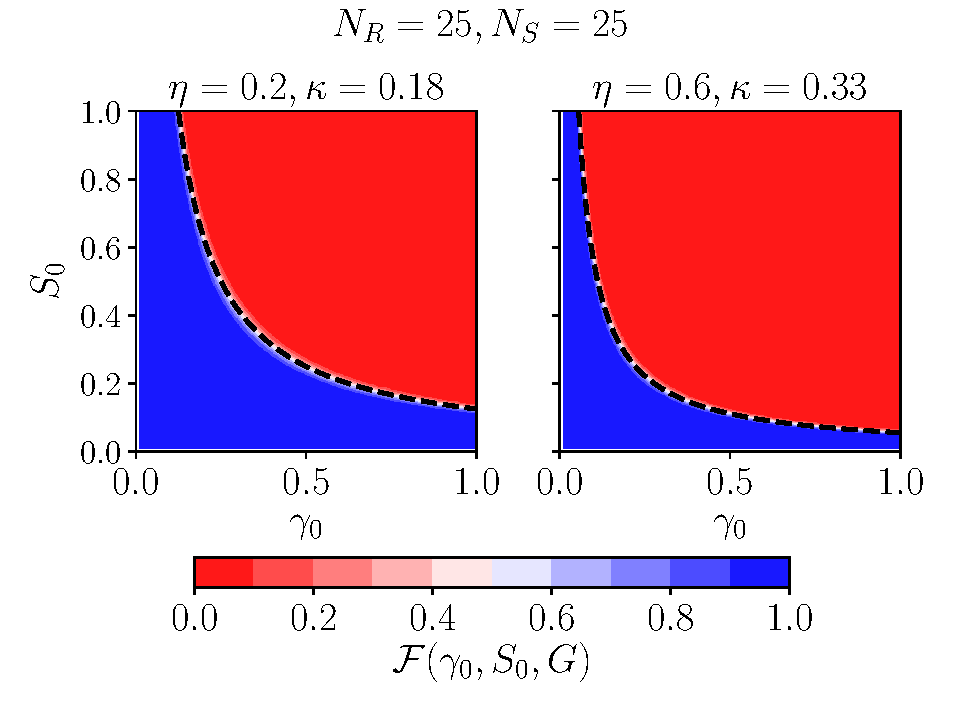
\includegraphics[width=0.7\linewidth]{typical_feasibility_volume}
\caption{Plot of the feasibility region in the absence of syntrophy. The color curve indicates the feasibility function $\mathcal{F}\left((\gamma_0, S_0, \alpha_0=0), G, 0\right)$ for $G_1$, which has a connectance $\kappa_{G}=0.18$ and ecological overlap $\eta_{G}=0.2$ (left) and $G_2$ with $\kappa_G=0.28$ and $\eta_G=0.4$(right). We observe a steep descent which marks a very clear transition from a totally feasible regime to a totally unfeasible regime, which allows us to precisely get the boundary of $\mathcal{F}^{G, 0}_1$. The dashed lines indicate the theoretical predictions.}
\label{fig: typical feasibility region}
\end{figure}
%of our set. $G_1$ has connectance $\kappa_1=0.17$ and nestedness $\eta_1=0.2$, $G_2$ is more connected and more nested: $\kappa_2=0.37$ and $\eta_2=0.4$.
We generally observe two distinct zones in the $(\gamma_0, S_0)$ space: full feasibility ($\mathcal{F}$ as defined in Eq.\eqref{eq : feasibility methods feasibility metaparameters function} is equal to $1$, blue part of Fig.\ref{fig: typical feasibility region}) and full unfeasibility ($\mathcal{F}=0$, red part). These two zones are separated by a narrow region of partial feasibility $0 <\mathcal{F}<1$. Since that region is very thin, we can define  the ``boundary'' line between feasibility and unfeasibility as the level\footnote{Numerically because of the possible noise, we take as part of the boundary every $(\gamma_0, S_0)$ such that $0.4 < \mathcal{F} <0.6$.} $\mathcal{F}=0.5$. Theoretically, that sharp transition between feasibility and unfeasibility happens when both sides of the inequality \eqref{eq: fully feasible volume no syntrophy} are equal, \ie at $\gamma_0 R_0 = l_0/\max_\nu\{\deg(G,\nu)\}S_0$. Hence we expect the boundary measured above to be well characterized by the curve $S_0 = K \gamma_0^{-1}$ with $K=l_0/(R_0 \max_\nu\left\{\deg(G,\nu)\right\})$.

 For $G_1$, the theoretical expectation is $S_0 = 0.125 \gamma_0^{-1}$ and a fit on the numerical results gives $S_0=(\num[scientific-notation=false]{0.124}\pm\num{3e-8}) \gamma_0^{-1}$ so the theoretical estimate is very accurate.
For $G_2$, we expect $S_0 = 0.077 \gamma_0^{-1}$. A fit gives $S_0=(\num[scientific-notation=false]{0.076}\pm\num{7e-9})\gamma_0^{-1}$. Again, the theoretical value is very close to the numerical measurement.
However, the numerical estimate does not always match the theoretical value that well. Figure \ref{fig: deviation away from theory feasibility} shows the relative error $\Delta_K \defined 1 - K_\text{theorical}/K_\text{fit}$. We see that in general $\Delta_K < 0$, \ie the theoretical expectation tends to overestimate the fully feasible region. This is probably due to noise (\ie coming from the difference between the metaparameters and the parameters) in the actual systems and the topology of the consumption matrix $G$. Figure \ref{fig: deviation away from theory feasibility} shows that the lower the ecological overlap or connectance of $G$, the worse the theoretical estimate. Finding a more accurate approximation which takes into account the deviations away from the metaparameters and the topology of $G$ remains a challenge for future studies.

\begin{figure}[h!]
	\captionsetup[subfigure]{captionskip = -175pt, margin = 45pt}
\subfloat[\label{fig: deviation away from theory feasibility fixed nestedness}]{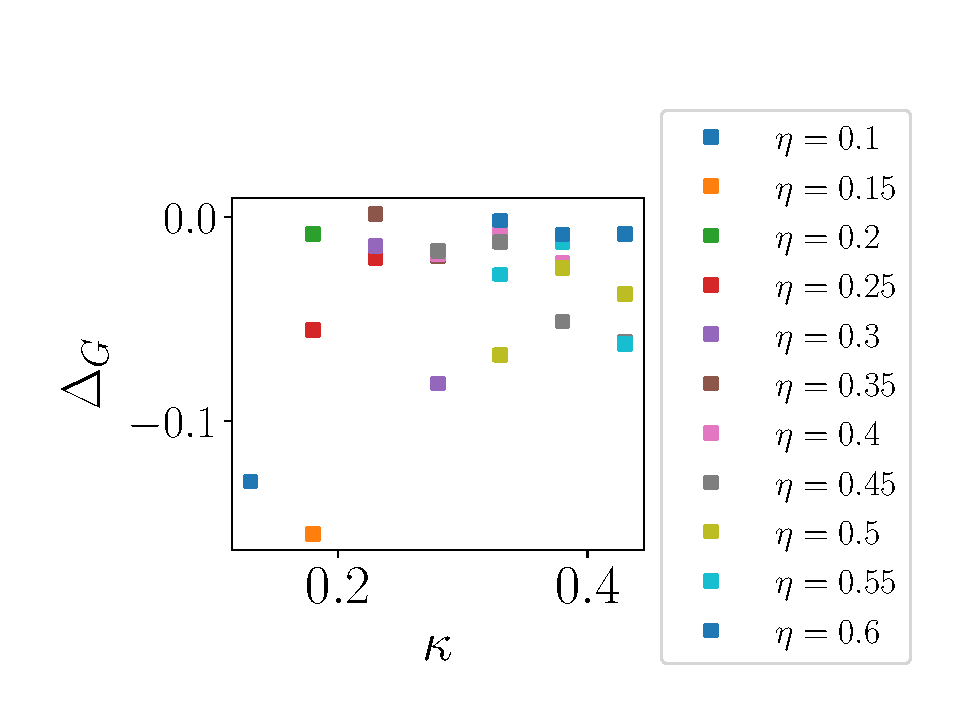
\includegraphics[width=0.49\linewidth]{feasibility_away_from_theory_fixed_nestedness}}
\captionsetup[subfigure]{captionskip = -175pt, margin = 45pt}
\subfloat[\label{fig: deviation away from theory feasibility fixed connectance}]{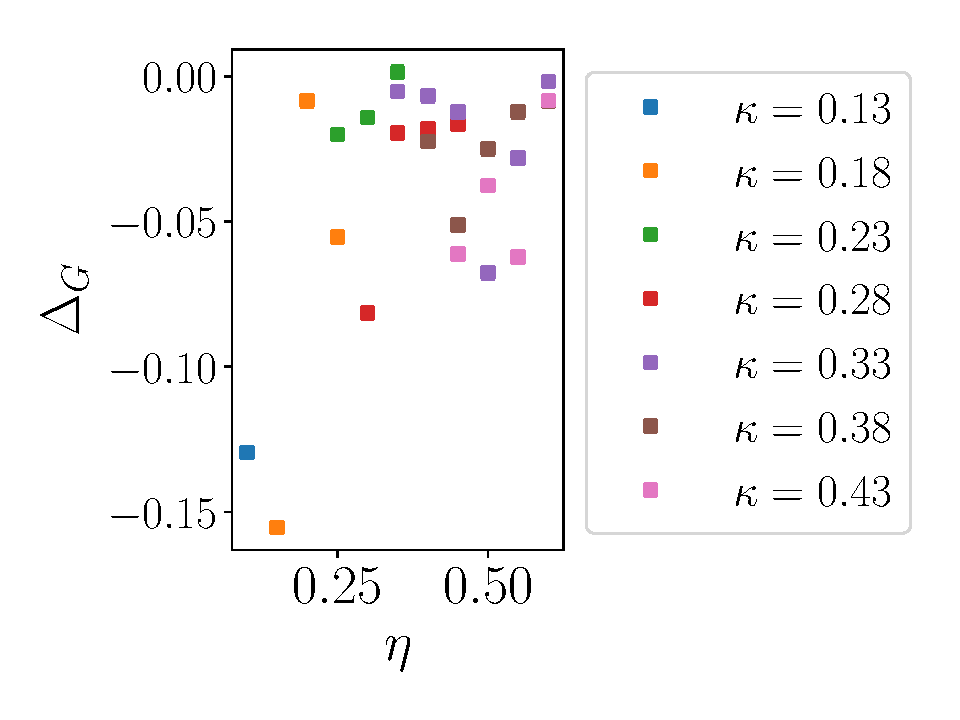
\includegraphics[width=0.49\linewidth]{feasibility_away_from_theory_fixed_connectance}}
\caption{Relative error in the determination of the boundary of $\mathcal{F}^{G,0}_1$. The curious reader may easily show that this is also the relative error on the area of $\mathcal{F}^{G,0}_1$. (a) varying connectance at fixed ecological overlap and (b) varying ecological overlap at fixed connectance. The theoretical prediction tends to overestimate the measured value. The larger the ecological overlap or connectance, the better the estimate.}\label{fig: deviation away from theory feasibility}
\end{figure}


We can similarly measure the common fully feasible volume in the absence of syntrophy $\mathcal{F}_1^{G_{25}}(0)$ (depicted in Fig.\ref{fig: common feasible volume no syntrophy}), which according to Eq.\eqref{eq: fully feasible volume no syntrophy} is inversely proportional to the largest maximal row degree of the matrix set. For the set $S_{25}$, this yields in theory: $S_0 = 0.053 \gamma_0^{-1}$. A fit on the points at the edge yields the critical boundary $S_0 = (0.042 \pm 10^{-8})\gamma_0^{-1}$, which is $\sim 21 \%$ away from the theoretical prediction. The discrepancy is probably due to the difference between the way we estimate the boundary numerically and analytically.
\begin{figure}[h!]
\centering
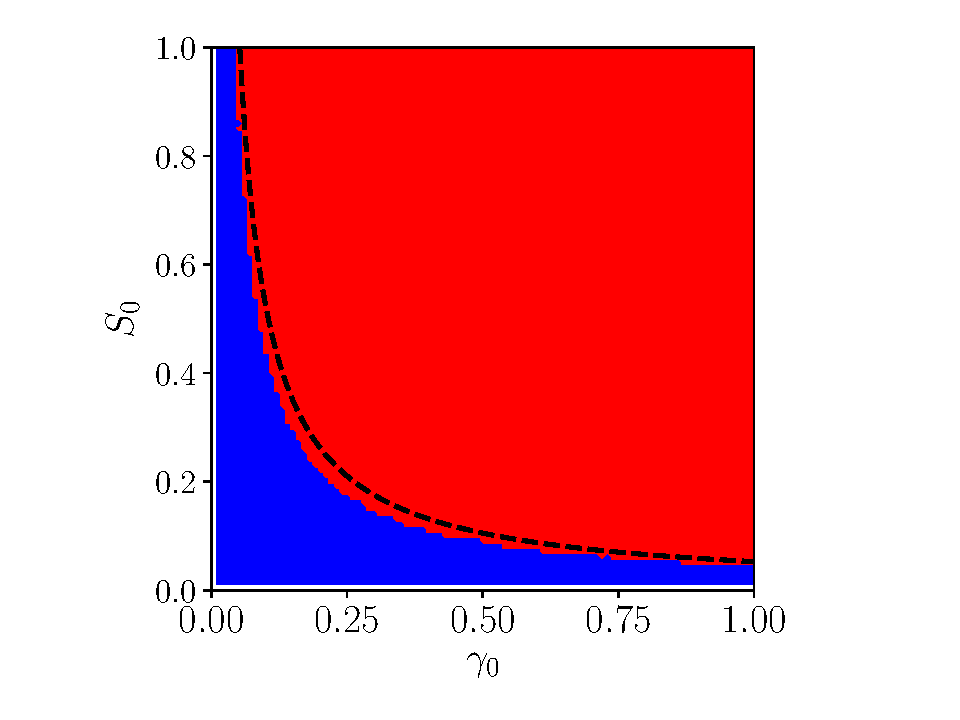
\includegraphics[width=0.6\linewidth]{common_feasibility_volume_no_syntrophy}
\caption{Plot of the common feasibility region. The blue area indicates the common feasibility volume, computed numerically, while the dashed line shows the analytical prediction. Although the match is not as good as before, the relative error is only of the order of $20 \%$. The red part is the area where not all matrices are fully feasible.}
\label{fig: common feasible volume no syntrophy}
\end{figure}

\FloatBarrier
\clearpage
\subsection{Impact of syntrophy on the feasible region}\label{sec: impact of syntrophy on feasible region}

Above we computed feasible volumes when there is no syntrophy \ie $\mathcal{F}^{G,0}_1$. Because there was no syntrophy, we did not need to specify what the structure of $A$ was. The next naturally arising question is then: what happens to the feasible region of a community with a given consumption matrix $G$ when we add a syntrophic interaction, \ie a syntrophic network $A$ of average interaction strength $\alpha_0$? More precisely, how does the shape of $\mathcal{F}^{G,A}_1$ change as a function of $A$ and $\alpha_0$?

A layer of complexity arises on top of the problem discussed above%. When we computed $\mathcal{V}^G_1(\alpha_0=0)$, we only had to take into account the structure of $G$, since there was no syntrophy. Now, we have an additional complexity because
: apart from the structure of the consumption matrix $G$, we now have to think about both the topology of $A$ and $\alpha_0$. As explained in Section \ref{sec : domain of study}, performing a detailed numerical study of the topology of $A$ would lead to a combinatorially unfeasible exploration, so we focus on the four $A$ cases enunciated above: ``fully connected'' (FC), ``no intraspecific syntrophy'' (NIS), ``LRI matrix'' (LRI), and ``random structure'' (RS). Concerning the question of $\alpha_0$, we would like to be ``fair'' among all networks and study syntrophy strengths that are feasible for all the consumption-syntrophy networks considered $(G,A) \in S_{25}$.
  The largest syntrophy compatible with full feasibility for all the networks considered, which we will refer to as \important{the largest common fully feasible syntrophy} $\alpha_C^F$ is the value of $\alpha_0$ such that $\mathcal{F}^{G,A}_1 \neq \emptyset $ $\forall (G,A) \in S_{25}$. It can be estimated with the help of Eq.\eqref{eq : fully feasible volume}:
  \begin{equation}
  \alpha_0 \lessapprox \frac{\min(1-\sigma_0, \sigma_0)R_0}{\max_{(G,A) \gamma_0 \in S}\left\{\max_i\left\{\frac{\deg(A,i)}{\deg(G,i)}\right\}\right\}} \gamma_0 \approx 0.01 \gamma_0 \leq 0.01. \label{eq : results feasibility largest alpha0}
  \end{equation}
  We will hence investigate the impact of $\alpha_0$ evaluated at ten different values from $0$ to $0.015$. %We first consider the effect of syntrophic interaction on each consumption network $G$ then on the common fully feasible volume.
  Since we do not change $\alpha_0$ in a continuous way but instead focus on different ``$\alpha_0$-slices'' of $\mathcal{F}^{G,A}_1$, the object of our attention is the set of $(\gamma_0, S_0)$ such that $(\gamma_0, S_0, \alpha_0) \in \mathcal{F}^{G,A}_1$. We will refer to it as $\mathcal{F}^{G,A}_1(\alpha_0)$:
  \begin{equation}
  \mathcal{F}^{G,A}_1(\alpha_0) \defined \left\{(\gamma_0, S_0) : (\gamma_0, S_0, \alpha_0) \in \mathcal{F}^{G,A}_1 \right\}.
  \end{equation}
  Because Equation \eqref{eq : fully feasible volume} depends on the structure of $G$ and of $A$, we expect $\mathcal{F}^{G,A}_1(\alpha_0)$ to depend heavily on the topology of both the consumption and syntrophy matrices.

  \subsubsection{The influence of matrix topology}\label{sec : feasibility results influence of matrix topology}
  Figure \ref{fig: feasibility results fully feasible volume different consumption matrices} shows that indeed $\mathcal{F}^{G,A}_1(\alpha_0)$ changes significantly not only with syntrophy $\alpha_0$ but also with the network structure of the consumption matrix $G$.
  \begin{figure}
  \captionsetup[subfigure]{captionskip = -195pt, margin=65pt}
  \hspace{-0.2\linewidth}
  \subfloat[\label{fig: feasibility results feasibility region eta 0.6 kappa 0.3 NR=25}]{\includegraphics[width=1.4\linewidth]{{feasibility_region_wt_wc_NR25_NS25_Nest0.6_Conn0.3168}.pdf}}

  \vspace{-60pt}
  \hspace{-0.2\linewidth}
  \subfloat[]{\includegraphics[width=1.4\linewidth]{{feasibility_region_wt_wc_NR25_NS25_Nest0.35_Conn0.2208}.pdf}}

  \vspace{-60pt}
  \hspace{-0.2\linewidth}
  \subfloat[]{\includegraphics[width=1.4\linewidth]{{feasibility_region_wt_NR25_NS25_Nest0.15_Conn0.1808}.pdf}}

  \caption{Fully feasible region in the $(\gamma_0,S_0) \in [0,1]^2$ unit square as a function of syntrophy for different consumption matrices $G$: (a)
  $\eta_G=0.6$, $\kappa_G=0.33$, (b) $\eta_G=0.35$, $\kappa_G=0.23$ and (c) $\eta_G=0.15$, $\kappa_G=0.18$.
  The white zone corresponds to points that are never fully feasible. The colour of a given point tells until which syntrophy that point is fully feasible, \eg
  a light blue point is fully feasible for $0 \leq \alpha_0 \leq \num{9.1e-3}$. The size of the feasibility regions depends heavily on the topology of the matrix, which makes the problem far from trivial.}\label{fig: feasibility results fully feasible volume different consumption matrices}
  \end{figure}
  %The way in which $\mathcal{F}^{G,A}_1(\alpha_0)$ changes as a function of $A$ is a more difficult question. \textbf{TO DO: explain that this will be studied later : put reference to new figure (how do df and alpha0 change from the null case)?}
  We observe a general trend among all matrices: as syntrophy increases, the fully feasible region in the unit square shrinks towards high $\gamma_0$. This can be explained with the LHS of Eq.\eqref{eq : fully feasible volume} which provides a lower bound to $\gamma_0$ when $\alpha_0 > 0$:
  \begin{equation}
  \gamma_0 \gtrapprox \frac{\max_i\left\{\frac{\deg(A,i)}{\deg(G,i)}\right\}}{\min(1-\sigma_0, \sigma_0) R_0} \alpha_0.
  \end{equation}
  The abundance of consumers $S_0$ has still an upper bound provided by the RHS of Eq.\eqref{eq : fully feasible volume} which goes as something close to\footnote{Mathematically the difficulty is that we cannot split the two terms of the RHS of \eqref{eq: upper bound S0 syntrophy}. If we assume deg$(A,\nu)$ is small, then $S_0 \lessapprox \sim \gamma_0^{-1}$.} $\gamma_0^{-1}$:
  \begin{equation}
 \gamma_0 R_0
  \lessapprox
   \min_\nu \left\{ \frac{l_0}{\deg(G,\nu) S_0} + \frac{\deg(A,\nu)}{\deg(G,\nu)}\alpha_0\right\}.\label{eq: upper bound S0 syntrophy}
  \end{equation}
  %Note that taking into account $\alpha_0 >0$ does not put a lower bound on $S_0$, such that at a fixed $\gamma_0$, every $S_0$ from $0$ to the upper boundary critical curve $\sim \gamma_0^{-1}$ discussed before remains a fully feasible point.
  So in general, as syntrophy increases, systems with a high consumption rate and a low consumers abundance at equilibrium will remain feasible, while other simply will not exist. %This makes sense intuitively:\textbf{TO DO: put explanation here}

  Because of that shift to the right,  $\mathcal{F}^{G,A}_1(\alpha_0)$ shrinks in size\footnote{Note that when we talk about the size of $\mathcal{F}^{G,A}_1(\alpha_0)$, it is understood relatively to the $(\gamma_0, S_0)\in [0,1]^2$ unit square. In fact we expect that new points also appear to the right of the $\gamma_0=1$ axis as can be seen by inspecting Eq.\eqref{eq : fully feasible volume}. However, because the larger the $\gamma_0$, the smaller the range of feasible $S_0$, this newly added feasible area should vanish quickly as $\gamma_0$ increases.}: as syntrophy is increased, the set of possible consumption rates and average consumers abundances is more restricted.
  Figure \ref{fig: feasibility results typical shrinkage of feasible volume} shows that typically the feasibility volume $\text{Vol}\left(\mathcal{F}_1^{G,A}(\alpha_0)\right)$, formally defined in Section \ref{app: how to measure volume}, decays in an exponential-like fashion as $\alpha_0$ increases.
  \begin{figure}
  \centering
  \includegraphics[width=0.6\linewidth]{{size_feasibility_region_NR25_NS25_Nest0.25_Conn0.2336}.pdf}
  \caption{Decay of the volume of the fully feasible region $\mathcal{F}^{G,A}_1(\alpha_0)$ for a matrix consumption $G$ with ecological overlap $\eta_G=0.25$ and connectance $\kappa_G=0.23$ on a logarithmic scale. The solid lines represent the exponential fit explained in the main text. The four different colors represent the four different structures considered for the syntrophy matrix. The decay of $\text{Vol}(\mathcal{F}^{G,A}_1(\alpha_0))$ seems well approximated by an exponential decay. A random syntrophy matrix (RS scenario) allows for a larger feasibility volume.}
  \label{fig: feasibility results typical shrinkage of feasible volume}
  \end{figure}
  This is a simple translation of the biological hindsight that, because of the physical considerations (conservation of biomass and positivity of the parameters) discussed above, the number of systems that can sustain a given syntrophic interaction strength decreases with that interaction strength, \ie no system can support an arbitrarily large syntrophy.
  The shrinkage of the feasibility volume can be quantified by defining the \define{feasibility decay rate} $d_F$, which is obtained by performing a non-linear regression to find the coefficients $c_1,c_2, d_F \in \mathbb{R}^+$ that satisfy best\footnote{In practice, standard functions of the \code{numpy} and \code{scipy} Python libraries are used to perform that fitting procedure.}:
  \begin{equation}
\text{Vol}\left(\mathcal{F}_1^{G,A}(\alpha_0)\right) \approx c_1 \exp{\left(-d_F \alpha_0\right)} - c_2. \label{eq: feasibility results fit feasible volume}
  \end{equation}
  The value of $d_F(G,A)$ tells us how fast the feasible volume shrinks for a given consumption-syntrophy couple $(G,A)$. In that sense $d_F(G,A)$ provides a measure of how good $(G,A)$ can sustain an increase in syntrophy. %\footnote{One could also desire to define a \define{critical feasible syntrophy} as the smallest syntrophy that gives a zero fully feasible volume. This would be a very interesting quantity to study and could be easily found as the root of the RHS of Eq.\eqref{eq: feasibility results fit feasible volume}. We tried doing this, because the errors on $d_F$ and on the two other fitting coefficients are already quite large (see the caption of Fig.\ref{fig: feasibility results feasibility decay rate vs matrix structure}), the errors on the critical feasible syntrophy we obtained were way too large, making our results essentially meaningless.}.
  If $d_F$ is low then the system can bear an increase of syntrophy and stay feasible. On the opposite, if $d_F$ is high, if syntrophy is increased too much, the microbial community will have to fundamentally change (\eg move to a $(G,A)$ configuration with a lower $d_F$) or it will become unfeasible, \ie at least one species will get extinct.

  Figure \ref{fig: feasibility results decay rate FC case} shows how $d_F(G,A)$ changes as a function of the structure of $G$, for $A$ fully connected, and Figure \ref{fig: feasibility results feasibility decay rate vs matrix structure} shows how $d_F$ changes when the structure of $A$ changes.
  \begin{figure}
  \captionsetup[subfigure]{captionskip=-190pt, margin=44pt}
  \hspace{-0.05\linewidth}
  \subfloat[]{\includegraphics[width=0.55\linewidth]{{feasibility_NR25_NS25_feasibility_decay_rate_fixed_nestedness_fully_connected}.pdf}}
  \subfloat[]{\includegraphics[width=0.55\linewidth]{{feasibility_NR25_NS25_feasibility_decay_rate_fixed_connectance_fully_connected}.pdf}}
  \caption{Feasibility decay rate $d_F(G,A)$ for $A$ fully connected and $(G,A)\in S_{25}$. (a) $d_F$ as a function of the connectance of $G$ for different fixed ecological overlaps and (b) $d_F$ as a function of the ecological overlap $\eta_G$ for fixed different connectances. A strong trend may be seen: at fixed ecological overlap, $d_F$ decreases with connectance and at fixed connectance it increases with ecological overlap. Since a small $d_F$ allows to sustain a larger syntrophy, microbial communities where syntrophic interactions play a large role will tend to have a high connectance of the consumption matrix and a low ecological overlap.}\label{fig: feasibility results decay rate FC case}
  \end{figure}
  \begin{figure}
  \captionsetup[subfigure]{captionskip=-180pt, margin=44pt}

  \vspace{-30pt}
  \hspace{-0.03\linewidth}
  \subfloat[]{\includegraphics[width=0.53\linewidth]{{feasibility_NR25_NS25_feasibility_decay_rate_dev_away_from_FC_fixed_nestedness_no_release_when_eat}.pdf}}
  \subfloat[]{\includegraphics[width=0.53\linewidth]{{feasibility_NR25_NS25_feasibility_decay_rate_dev_away_from_FC_fixed_connectance_no_release_when_eat}.pdf}}

  \vspace{-12pt}
  \hspace{-0.03\linewidth}
  \subfloat[]{\includegraphics[width=0.53\linewidth]{{feasibility_NR25_NS25_feasibility_decay_rate_dev_away_from_FC_fixed_nestedness_optimal_matrix}.pdf}}
  \subfloat[]{\includegraphics[width=0.53\linewidth]{{feasibility_NR25_NS25_feasibility_decay_rate_dev_away_from_FC_fixed_connectance_optimal_matrix}.pdf}}

  \vspace{-12pt}
  \hspace{-0.03\linewidth}
  \subfloat[]{\includegraphics[width=0.53\linewidth]{{feasibility_NR25_NS25_feasibility_decay_rate_dev_away_from_FC_fixed_nestedness_random_structure}.pdf}}
  \subfloat[]{\includegraphics[width=0.53\linewidth]{{feasibility_NR25_NS25_feasibility_decay_rate_dev_away_from_FC_fixed_connectance_random_structure}.pdf}}
  \vspace{-6pt}
  \caption{Relative difference of the feasibility decay rate for the considered $A$ scenario compared to the FC null case (Fig.\ref{fig: feasibility results decay rate FC case}) for $N_R=25$ and $N_S=25$. Plots on the first column (a)-(c)-(e) show how that quantity changes with connectance for a given ecological overlap, while plot on the second column (b)-(d)-(f) show how it evolves when ecological overlap is changed and connectance is kept fixed. Different structures of the $A$ matrix are considered: (a)-(b) NIS, (c)-(d) LRI (e)-(f) RS. A positive $y$-coordinate means that for the feasibility decay rate of the current syntrophy scenario is smaller than for the FC case, \ie the system sustains syntrophy better with the considered $A$-structure compared to fully connected. The FC scenario is always outperformed by the other scenarios, especially the random structure (RS) case.}\label{fig: feasibility results feasibility decay rate vs matrix structure}
  \end{figure}
  %Interestingly, the structure of $A$ does not provide any real difference, except for $G$ with $\eta_G=0.15$ and $\kappa_G=0.18$. For that specific matrix, the LRI scenario for $A$ reduced by a factor of three the decay rate, compared to the fully connected case. That result is only true for this specific matrix and does not hold for the others, where $d_F(G,A)$ seems to almost not depend on $A$.
  A very strong trend can be observed as a function of the consumption matrices%and all structures of $A$
  : for a given connectance $\kappa_G$, $d_F$ is increased if the ecological overlap $\eta_G$ is increased and for a given ecological overlap, $d_F$ decreases if the connectance is increased.
  In biological terms, systems where there is a small ecological overlap (\ie small competition) but a lot of links in the food consumption network will be favoured. Microbial communities where consumers on average eat from a lot of different resources (\ie each their own) can sustain a larger syntrophic interaction than others. The shape of the syntrophy matrix changes the feasibility decay rate in a non-trivial way. An NIS structure significantly (we observe up to a $50\%$ percent difference) decreases $d_F$; the improvement is better for larger $\kappa_G$ and lower $\eta_G$. The LRI scenario has a suprising effect: for low $\kappa_G$, $d_F$ is significantly lowered (almost by $100\%$ in the best case) but for $\kappa_G > 0.23$, there is no improvement. Finally the RS scenario offers the best improvement: $d_F$ is improved by at least $50\%$ for all networks. Note that the underlying trend is very regular: for a fixed connectance $\kappa_G$, the improvement is almost $100\%$ at low ecological overlap. As $\eta_G$ increases, the improvement decreases until it saturates and stays constant. The saturation value is larger when $\kappa_G$ is smaller. The regularity of such results suggests an underlying analytical explanation that has yet to be derived.

  %Such a fit also allows to find the \define{critical feasible syntrophy $\alpha_0^F(G,A)$}, which we define as the smallest syntrophy for which the fully feasible volume is zero. Indeed, one finds $\alpha_0^F$ by looking at the intercept of Eq.\eqref{eq: feasibility results fit feasible volume} with the $x$-axis:
  % \begin{equation}
  % \alpha_0^F(G,A) \defined -\frac{1}{c_2} \ln\left({\frac{c_3}{c_1}}\right).
  % \end{equation}

  \subsubsection{Common fully feasible volume}
 After studying the effect of syntrophy on each consumption-syntrophy network $(G,A)$, we can focus on the overlap of all the fully feasible regions: the common fully feasible region $\mathcal{F}_1^{S_{25}}\defined \intersection{(G,A)\in S_{25}} \mathcal{F}^{G,A}_1$. Similarly to above, we slightly abuse notation and write:
\begin{equation}
\mathcal{F}_1^{S_{25}}(\alpha_0) \defined \left\{(\gamma_0, S_0) : (\gamma_0, S_0, \alpha_0) \in \mathcal{F}_1^{S_{25}}\right\}.
\end{equation}
 Figure \ref{fig: results feasibility cfv variation with syntrophy} shows the evolution of $\mathcal{F}_1^{S_{25}}(\alpha_0)$ as syntrophy increases. %Once again, the structure of $A$ does not seem to play a significant role in the shape of $\mathcal{F}_1^{S_{25}}(\alpha_0)$. Note that $\text{Vol}\left(\mathcal{F}_1^{S_{25}}\left(\alpha_0=\num{9.1e-3}\right)\right)=0$ but at $\alpha_0=\num{7.8e-3}$ the common feasible region is still non-zero. So the largest common fully feasible syntrophy $\alpha_C^F(S_{25})$ established in Eq.\eqref{eq : results feasibility largest alpha0} as $\sim 0.01$, lies between \num{7.8e-3} and \num{9.1e-3}, which shows that the order of magnitude is theoretically correctly estimated.
 In accordance to what was observed individually for each matrix before, the RS scenario allows for a larger syntrophy: at a given $\alpha_0$, there are more feasible $(\gamma_0, S_0)$ points if $A$ has a random structure. The three other scenarios do not offer a significant difference and at $\alpha_0=\num{9.1e-3}$ there are no more $(\gamma_0, S_0)$ that are fully feasible for all matrices. This means that the largest common fully feasible syntrophy respects $\num{7.8e-3}<\alpha_C^F \leq \num{9.1e-3}$ for those three scenarios, which puts the estimate $\alpha_C^F \approx 0.01$ of Eq.\eqref{eq : results feasibility largest alpha0} not far from the numerical bounds.

Without surprise, $\text{Vol}\left(\mathcal{F}_1^{S_{25}}(\alpha_0)\right)$ also decays in an exponential-like fashion as is shown by Figure \ref{fig: feasibility results volume of cfr depending on syntrophy}.
\begin{figure}[h!]
% \captionsetup[subfigure]{captionskip = -185pt, margin = 195pt}
%
% \hspace{-0.1\linewidth}
% \subfloat[]{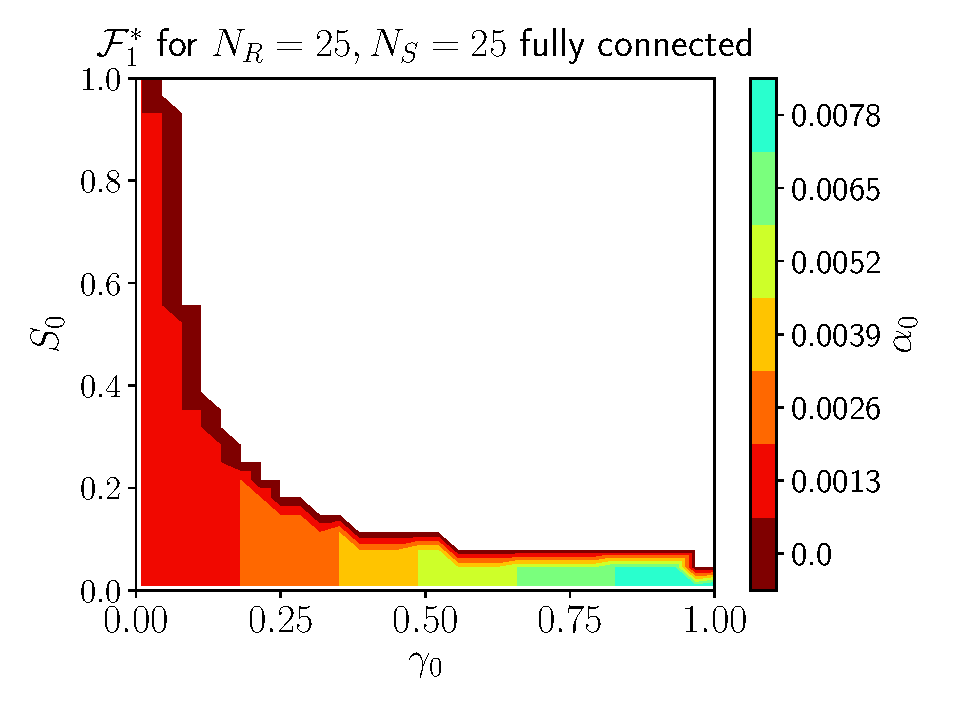
\includegraphics[width=0.6\linewidth]{common_feasibility_volume_NR25_NS25_varying_syntrophy_random_structure}}
% \subfloat[]{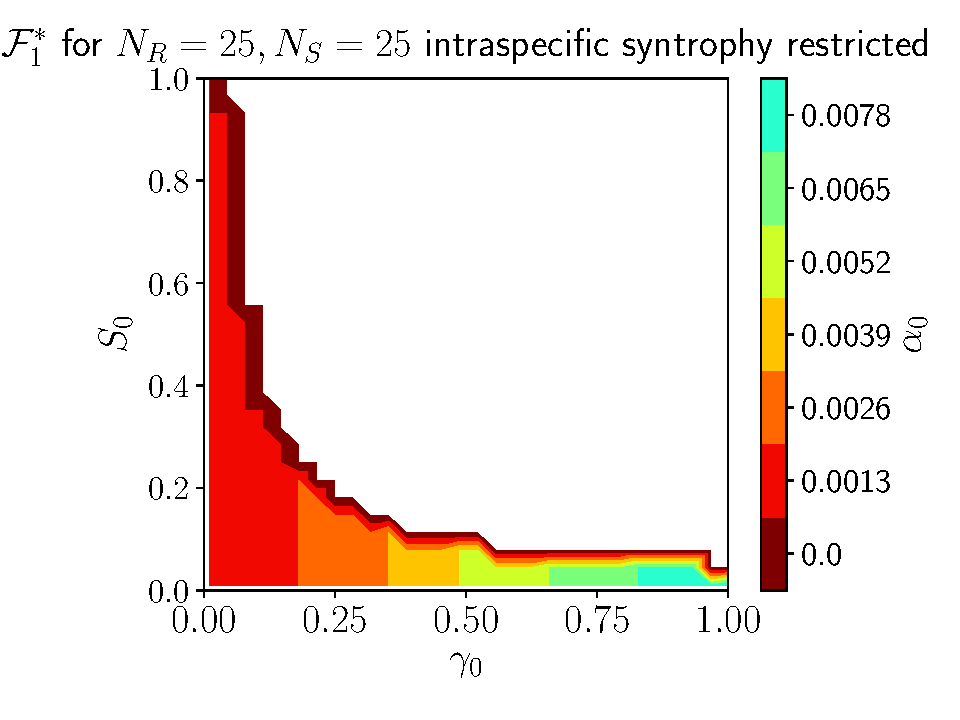
\includegraphics[width=0.6\linewidth]{common_feasibility_volume_NR25_NS25_varying_syntrophy_no_release_when_eat}}
%
% \centering
% \subfloat[]{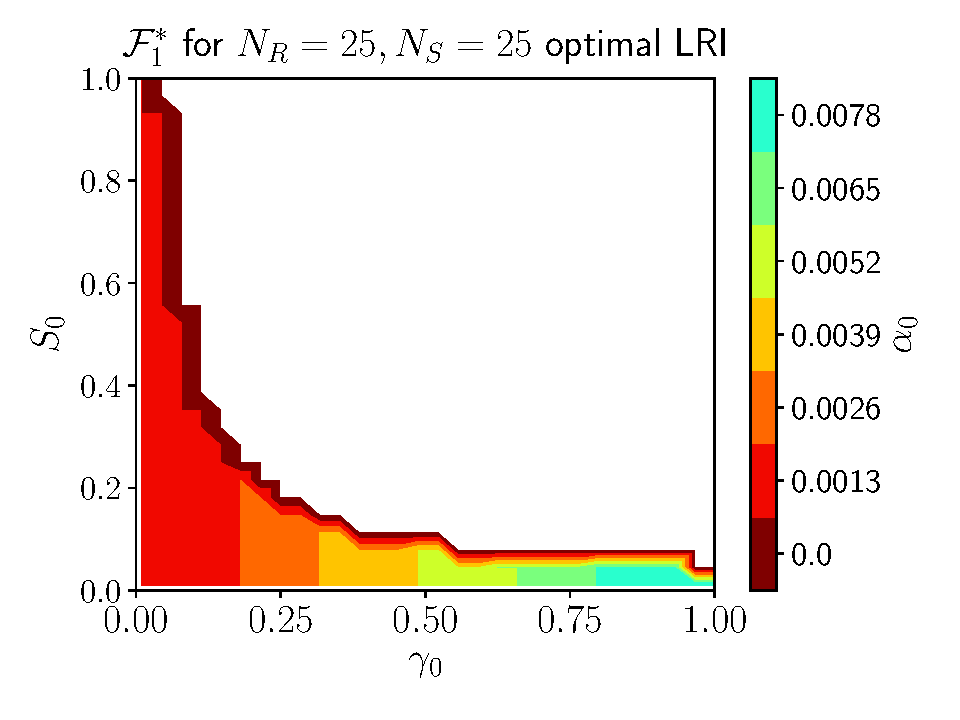
\includegraphics[width=0.6\linewidth]{common_feasibility_volume_NR25_NS25_varying_syntrophy_optimal_matrix}}
\hspace{-0.2\linewidth}
\includegraphics[width=1.4\linewidth]{{common_feasibility_region_NR25_NS25}.pdf}

\caption[caption for LOF]{Surface plot of the fully feasible volume $\mathcal{F}^{S_{25}}_1(\alpha_0)$. The color bar on the side indicates the value of $\alpha_0$ to which the surface corresponds. The white part of the plot corresponds to points that \important{never} are fully feasible. Note that even though it is not very clear on the figure $\mathcal{F}_1^{S_{25}}(\alpha_0^+) \subset \mathcal{F}_1^{S_{25}}(\alpha_0^-) \ \forall \alpha_0^+ > \alpha_0^-$, \ie the common fully feasible region of higher syntrophy is included in the one of lower syntrophy. The different subplots correspond to the different structures of the syntrophy matrix.} \label{fig: results feasibility cfv variation with syntrophy}
\end{figure}
\begin{figure}
\centering
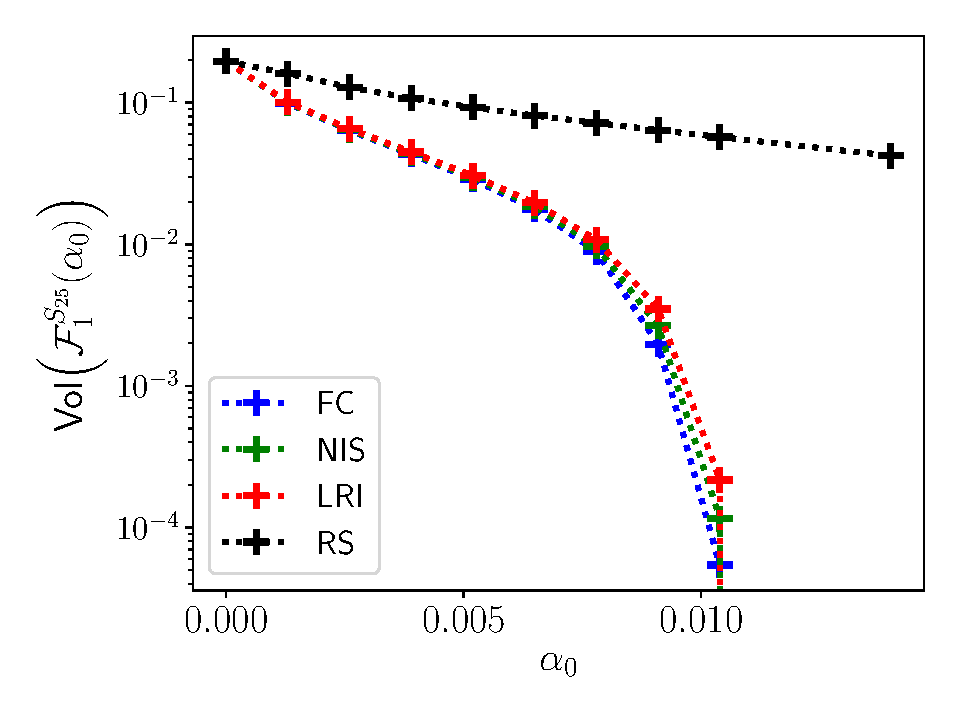
\includegraphics[width=0.65\linewidth]{common_feasibility_volume_NR25_NS25}
\caption{Volume of the common feasibility region $\mathcal{F}^{S_{25}}_1(\alpha_0)$ as a function of syntrophic interaction strength $\alpha_0$ (plotted on logarithmic scale). While the FC, NIS and LRI cases offer similar results, the RS scenario outperforms all of them. An exponential fit (Eq.\ref{eq: feasibility results fit feasible volume}) allows to measure a global $d_F$ for each of the four scenarios. The global decay feasibility rate of the RS scenario is 3 times smaller than the others.}\label{fig: feasibility results volume of cfr depending on syntrophy}
\end{figure} %with a rate $d_F(S_M)=\num[scientific-notation=false]{480(50)}$ per unit of syntrophy which is a bit larger than the largest $d_F(G,A)$ observed in Fig.\ref{fig: feasibility results feasibility decay rate vs matrix structure}.
An exponential fit\footnote{We take as error the standard deviation produced by the \code{scipy} routine we used.} allows to find the feasibility decay rates of each scenario: for the FC case, $d_F=\num[scientific-notation=false]{480(42)}$ (in units of syntrophy $\alpha_0$); for NIS, $d_F=\num[scientific-notation=false]{463(43)}$; for LRI, $d_F=\num[scientific-notation=false]{450(42)}$ and finally for RS, $d_F=\num[scientific-notation=false]{139(33)}$. The FC, NIS and LRI scenarios of $A$ do not produce a significant difference in feasibility. However a random $A$-matrix (RS scenario) allows for a 3 times smaller feasibility decay rate and hence at a given syntrophy $\alpha_0$, for many more pairs of common feasible $(\gamma_0, S_0)$.
Again we observe the same shift of $\mathcal{F}_1^{S_{25}}$ towards points with a high $\gamma_0$ and consequently a small $S_0$. Overall, independently of the consumption-syntrophy network structure, microbial communities which have a low abundance and high uptake rates can sustain a larger syntrophy than others. Among these, the ones which have a random syntrophy network are the most ``compatible'' with even larger syntrophic interaction.


\FloatBarrier
\subsubsection{The influence of the matrix dimensions}
We focused above on microbial communities with the same number of consumers and resources: $N_R=N_S=25$. But such systems lie at what has been referred to in the literature as May's stability bound \cite{biroli_marginally_2018}, which is defined as an ecological community where the number of resources is equal to the number of species. According to the competitive exclusion principle\footnote{The heavily debated and often misunderstood \cite{hardin_competitive_1960} \important{competitive exclusion principle}, also known as Gause's principle, states that ``Complete competitors cannot coexist'' \cite{hardin_competitive_1960}, or more generally that ``the number of consumer species in steady coexistence cannot exceed that of resources'' \cite{wang_overcome_2019}.}, an ecological system which has as many resources as consumers is the limiting case where coexistence, \ie feasibility in the terms used here, starts to exist. In a way, the study conducted before can be seen as a borderline case and it can be very fruitful to investigate the behaviour of systems where the number of resources has been increased to $N_R=50$.

% Figure \ref{fig: feasibility results typical feasible volumes NR=50 NS=25} is the $N_R=50$ equivalent to Figure \ref{fig: feasibility results fully feasible volume different consumption matrices}.
% \begin{figure}
% \captionsetup[subfigure]{margin=40pt}
% \hspace{-0.15\linewidth}
% \subfloat[\label{fig: feasibility results feasibility region eta 0.6 kappa 0.3}]{\includegraphics[width=1.3\linewidth]{{feasibility_region_wt_NR50_NS25_Nest0.6_Conn0.3344}.pdf}}
%
% \vspace{-55pt}
% \hspace{-0.15\linewidth}
% \subfloat[]{\includegraphics[width=1.3\linewidth]{{feasibility_region_wt_NR50_NS25_Nest0.35_Conn0.2296}.pdf}}
%
% \vspace{-55pt}
% \hspace{-0.15\linewidth}
% \subfloat[\label{fig: feasibility results feasibility region eta 0.15 kappa 0.12}]{\includegraphics[width=1.3\linewidth]{{feasibility_region_wt_NR50_NS25_Nest0.15_Conn0.12}.pdf}}
% \vspace{-12pt}
% \caption{Surface colour plot of the fully feasible region $\mathcal{F}_1^{G,A}\left(\alpha_0\right)$ as a function of the syntrophy $\alpha_0$ for the case $N_R=50$, with different structures of $A$: fully connected (left column), no intraspecific syntrophy (middle) and LRI matrix (right). The rows correspond to different choices of the consumption matrix $G$: (a) $\eta_G=0.6$ and $\kappa_G=0.33$, (b) $\eta_G=0.35$ and $\kappa_G=0.23$, (c) $\eta_G=0.15$ and $\kappa_G=0.13$. These are matrices with similar properties than  Fig.\ref{fig: feasibility results fully feasible volume different consumption matrices}, except that the number of resources is here doubled. This affects $\mathcal{F}_1^{G,A}\left(\alpha_0\right)$ quite drastically.}\label{fig: feasibility results typical feasible volumes NR=50 NS=25}
% \end{figure}
% We observe that increasing $N_R$ in general increases . For instance, for $G$ with $\eta_G=0.6$ and $\kappa_G=0.32$, adding more resources increases the maximal syntrophy bearable by the system (Fig.\ref{fig: feasibility results feasibility region eta 0.6 kappa 0.3} compared to Fig.\ref{fig: feasibility results feasibility region eta 0.6 kappa 0.3 NR=25}). On the contrary, for $G$ with $\eta_G=0.15$ and $\kappa_G=0.12$, it decreases it from \num{1.4e-2} to \num{7.8e-3}.

Figure \ref{fig: feasibility results common feasibility region NR=50 NS=25} shows the common feasibility region $\mathcal{F}_1^{S_{50}}$ of the $N_R=50$ matrix set $S_{50}$, which is to be compared with the common feasibility region for $N_R=25$ (Fig.\ref{fig: results feasibility cfv variation with syntrophy}). It seems that, independently of the structure of the $A$-matrix, a lesser common maximal syntrophy can be attained when the number of resources is doubled.
\begin{figure}[h!]
% \captionsetup[subfigure]{captionskip = -185pt, margin = 195pt}
%
% \hspace{-0.1\linewidth}
% \subfloat[]{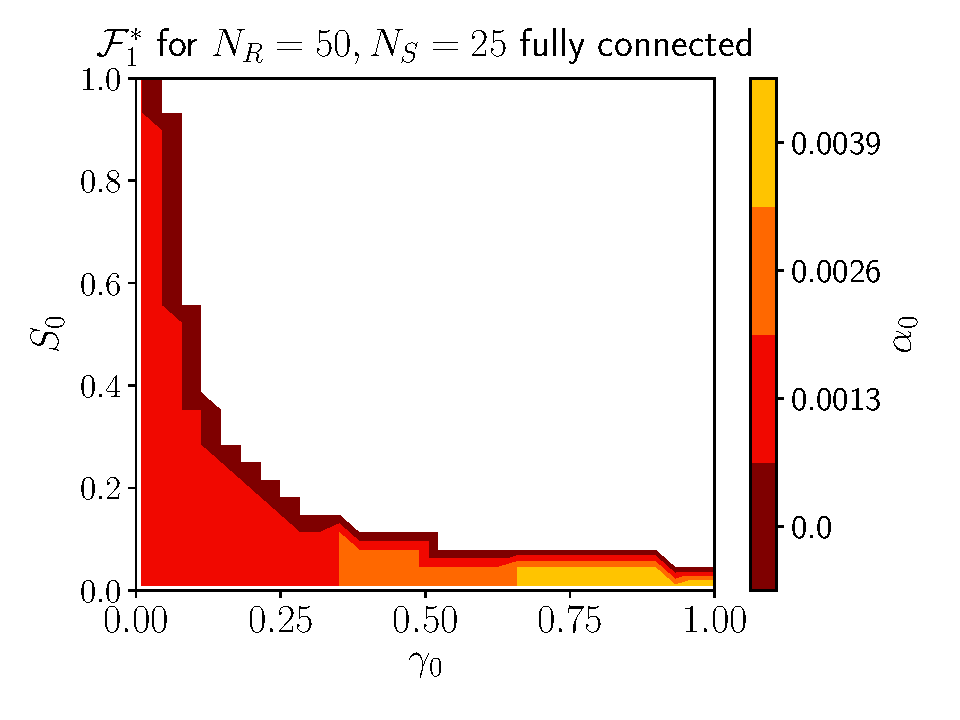
\includegraphics[width=0.6\linewidth]{common_feasibility_volume_NR50_NS25_varying_syntrophy_random_structure}}
% \subfloat[]{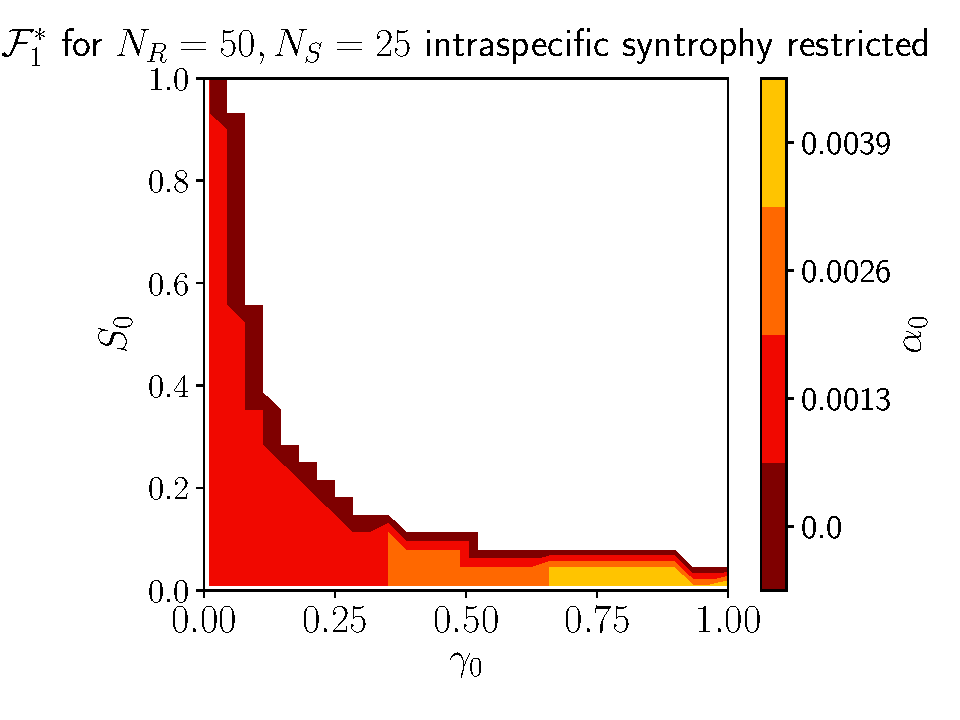
\includegraphics[width=0.6\linewidth]{common_feasibility_volume_NR50_NS25_varying_syntrophy_no_release_when_eat}}
%
% \centering
% \subfloat[]{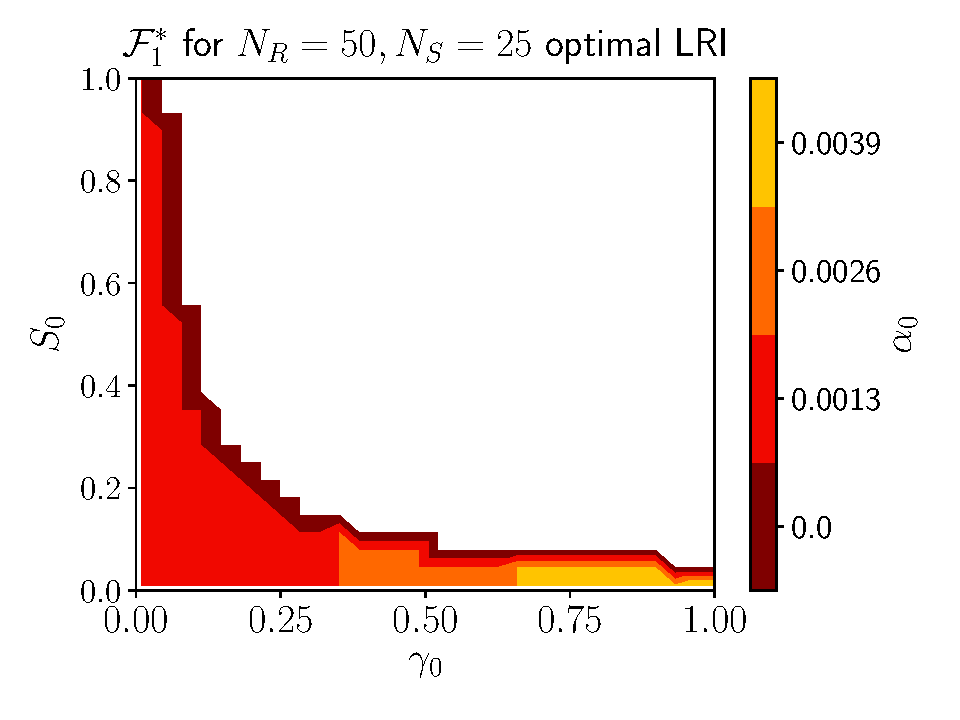
\includegraphics[width=0.6\linewidth]{common_feasibility_volume_NR50_NS25_varying_syntrophy_optimal_matrix}}
\hspace{-0.2\linewidth}
\includegraphics[width=1.4\linewidth]{{common_feasibility_region_NR50_NS25}.pdf}
\caption{Common feasibility region $\mathcal{F}_1^{S_{50}}\left(\alpha_0\right)$ for $N_R=50$ and $N_S=25$, to compare with \ref{fig: results feasibility cfv variation with syntrophy}. We considered four different structures of the syntrophy matrix: FC, NIS, LRI and RS. As the number of resources increases, the feasibility volume for a given $\alpha_0$ decreases.}\label{fig: feasibility results common feasibility region NR=50 NS=25}
\end{figure}
% We see that, compared with the $N_R=25$ case (Fig.\ref{fig: results feasibility cfv variation with syntrophy}), an overall lesser syntrophy can be achieved: the largest common fully feasible syntrophy is reduced \textbf{TO DO: put prediction here}. Finally Figure \ref{fig: feasibility results feasibility decay rate NR=50 NS=25} shows that indeed it is really hard to predict the effect that increasing the number of resources will have on a specific consumption-syntrophy network.

\noindent This might be the indication that changing $N_R$ modifies feasibility in a non-trivial way: the fact that the common feasibility region is different implies that the feasibility regions $\mathcal{F}_1^{G,A}$ change for all networks $(G,A)$ when $N_R=50$.
To quantify the effect on each individual consumption-syntrophy network, we may compute the decay feasibility rate and compare it to its counterpart when $N_R=25$. Figure \ref{fig: feasibility results feasibility decay rate NR=50 NS=25} shows that there is no clear pattern on how $d_F$ evolves when the number of resources is changed. Overall, the average ratio of the decay rates among the networks is equal to $\sim 1$: one could say that doubling the resources has on average no effect. Keep in mind that this conclusion should be carefully dealt with: although the matrices generated indeed do have the same connectance and ecological overlap, they may be different according to a measure that we have not monitored but which could be relevant biologically. This would mean that comparing the networks at $N_R=50$ and $N_R=25$ may not be fair. In the end, the parameter that controls how feasibility changes when the number of resources is modified is still unknown.

\begin{figure}
\captionsetup[subfigure]{captionskip=-202pt, margin=45pt}
\hspace{-0.1\linewidth}
\subfloat[]{\includegraphics[width=0.6\linewidth]{{feasibility_decay_rate_50_vs_25_fixed_connectance_fully_connected}.pdf}}
\subfloat[]{\includegraphics[width=0.6\linewidth]{{feasibility_decay_rate_50_vs_25_fixed_nestedness_fully_connected}.pdf}}


\caption{Ratio of the feasibility decay rates at $N_R=25$ and at $N_R=50$ as a function of the consumption matrix properties. A $y$-axis larger than $1$ means $d_F(N_R=25)$ is larger than $d_F(N_R=50)$, which means the system endures the addition of syntrophic interaction better at $N_R=50$. We considered the four usual $A$ scenarios (a)-(b) FC, and on the page below, (c)-(d) NIS, (e)-(f) LRI and (g)-(h) RS. Increasing the number of resources in the system does not allow microbial communities to be ``more feasible'' as syntrophy increases: on average $d_F$ is unchanged by doubling the number of resources. A detailed on how the consumption matrix properties, at least connectance and ecological overlap, or the $A$-scenario precisely modify the improvement is difficult to draw from this data.}
\label{fig: feasibility results feasibility decay rate NR=50 NS=25}
\end{figure}
\begin{figure}
\ContinuedFloat
\captionsetup[subfigure]{captionskip=-202pt, margin=45pt}

\hspace{-0.08\linewidth}
\subfloat[]{\includegraphics[width=0.58\linewidth]{{feasibility_decay_rate_50_vs_25_fixed_connectance_no_release_when_eat}.pdf}}
\subfloat[]{\includegraphics[width=0.58\linewidth]{{feasibility_decay_rate_50_vs_25_fixed_nestedness_no_release_when_eat}.pdf}}

\hspace{-0.08\linewidth}
\subfloat[]{\includegraphics[width=0.58\linewidth]{{feasibility_decay_rate_50_vs_25_fixed_connectance_optimal_matrix}.pdf}}
\subfloat[]{\includegraphics[width=0.58\linewidth]{{feasibility_decay_rate_50_vs_25_fixed_nestedness_optimal_matrix}.pdf}}

\vspace{-12pt}
\hspace{-0.08\linewidth}
 \subfloat[]{\includegraphics[width=0.58\linewidth]{{feasibility_decay_rate_50_vs_25_fixed_connectance_random_structure}.pdf}}
 \subfloat[]{\includegraphics[width=0.58\linewidth]{{feasibility_decay_rate_50_vs_25_fixed_nestedness_random_structure}.pdf}}
\caption{Continuation of the Figure above.}
\end{figure}
\FloatBarrier
%\documentclass[12pt, titlepage]{report}
\usepackage{consumer_resource_final}
\graphicspath{{./figures/}}

\begin{document}
\begin{figure}[h!]
\centering
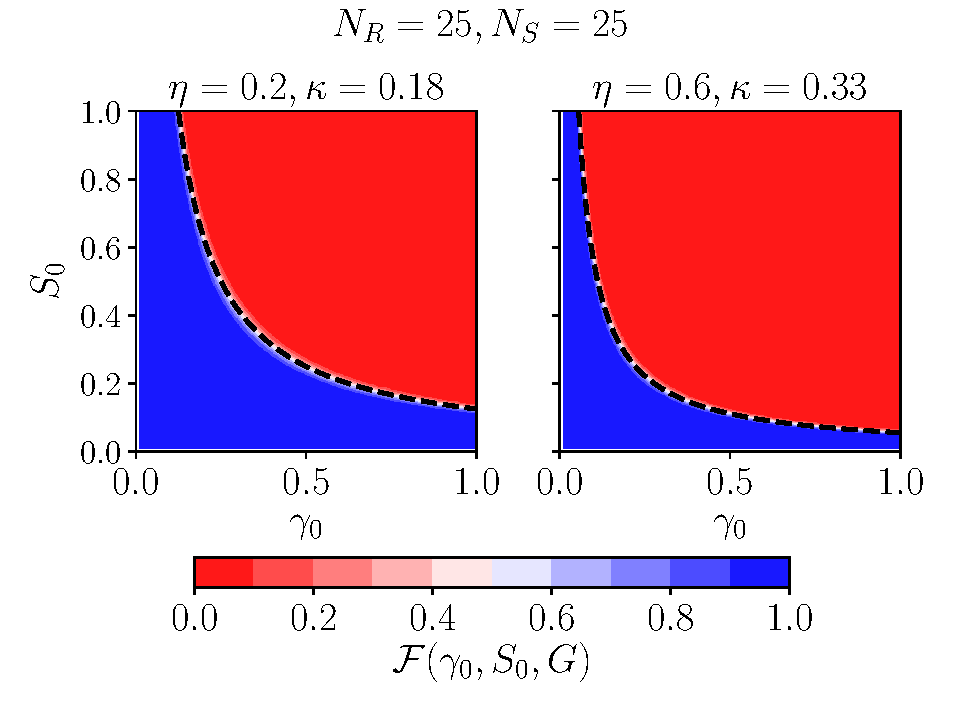
\includegraphics[width=0.7\linewidth]{typical_feasibility_volume}
\caption{Plot of the feasibility region in the absence of syntrophy. The color curve indicates the feasibility function $\mathcal{F}\left((\gamma_0, S_0, \alpha_0=0), G, 0\right)$ for $G_1$, which has a connectance $\kappa_{G}=0.18$ and ecological overlap $\eta_{G}=0.2$ (left) and $G_2$ with $\kappa_G=0.28$ and $\eta_G=0.4$(right). We observe a steep descent which marks a very clear transition from a totally feasible regime to a totally unfeasible regime, which allows us to precisely get the boundary of $\mathcal{F}^{G, 0}_1$. The dashed lines indicate the theoretical predictions.}
\label{fig: typical feasibility region}
\end{figure}
\begin{figure}[h!]
	\captionsetup[subfigure]{captionskip = -165pt, margin = 45pt}
\subfloat[\label{fig: deviation away from theory feasibility fixed nestedness}]{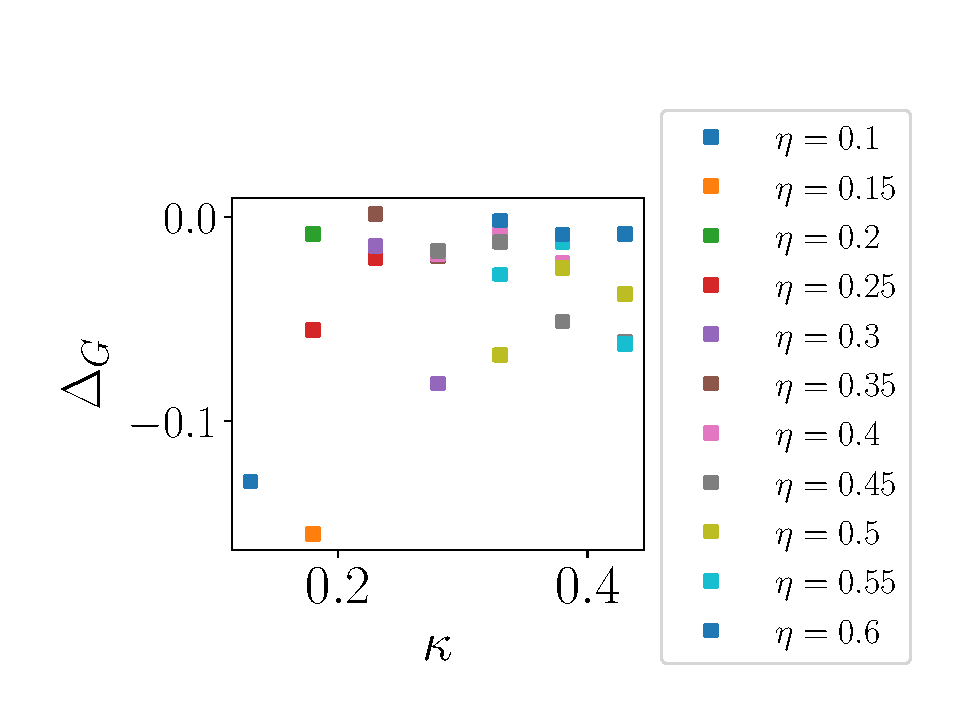
\includegraphics[width=0.49\linewidth]{feasibility_away_from_theory_fixed_nestedness}}
\captionsetup[subfigure]{captionskip = -175pt, margin = 45pt}
\subfloat[\label{fig: deviation away from theory feasibility fixed connectance}]{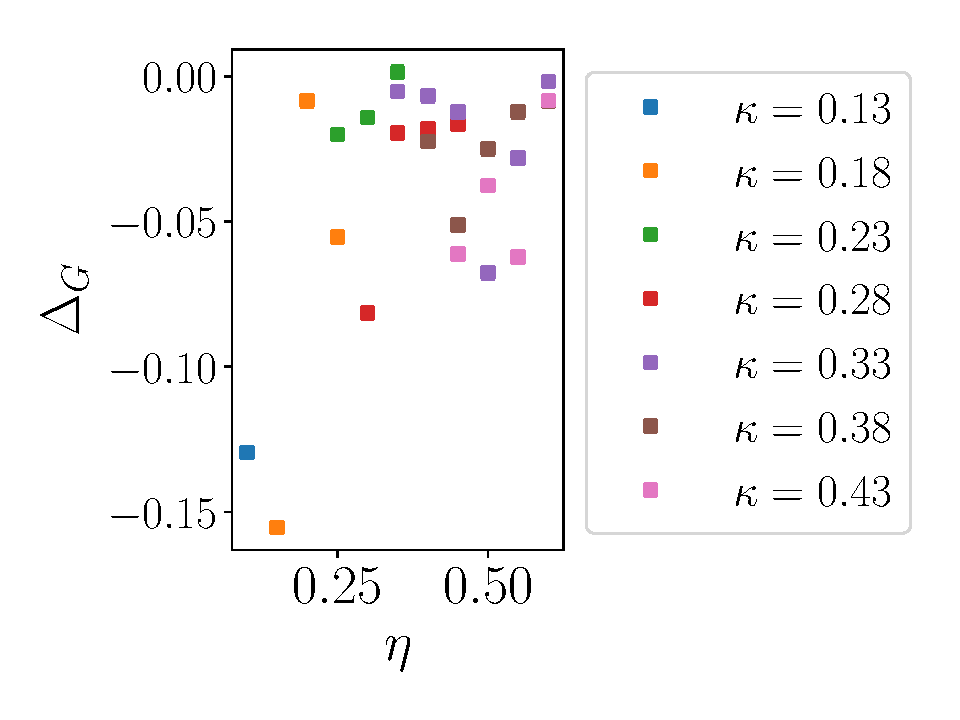
\includegraphics[width=0.49\linewidth]{feasibility_away_from_theory_fixed_connectance}}
\caption{Relative error in the determination of the boundary of $\mathcal{F}^{G,0}_1$ (a) varying connectance at fixed ecological overlap and (b) varying ecological overlap at fixed connectance. The theoretical prediction tends to overestimate the measured value. The larger the ecological overlap or connectance, the better the estimate.}\label{fig: deviation away from theory feasibility}
\end{figure}
\begin{figure}[h!]
\centering
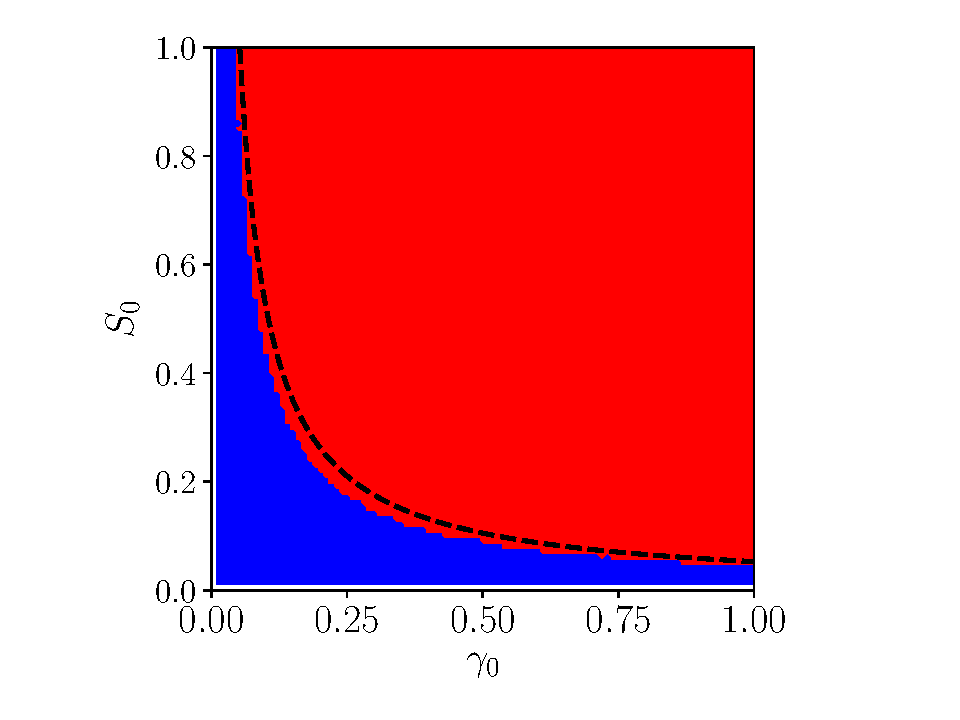
\includegraphics[width=0.6\linewidth]{common_feasibility_volume_no_syntrophy}
\caption{Plot of the common feasibility region. The blue area indicates the common feasibility volume, computed numerically, while the dashed line shows the analytical prediction. Although the match is not as good as before, the relative error is only of the order of $20 \%$. The red part is the area where not all matrices are fully feasible.}
\label{fig: common feasible volume no syntrophy}
\end{figure}
\begin{figure}
\captionsetup[subfigure]{captionskip = -195pt, margin=65pt}
\hspace{-0.2\linewidth}
\subfloat[\label{fig: feasibility results feasibility region eta 0.6 kappa 0.3 NR=25}]{\includegraphics[width=1.4\linewidth]{{feasibility_region_wt_wc_NR25_NS25_Nest0.6_Conn0.3168}.pdf}}

\vspace{-60pt}
\hspace{-0.2\linewidth}
\subfloat[]{\includegraphics[width=1.4\linewidth]{{feasibility_region_wt_wc_NR25_NS25_Nest0.35_Conn0.2208}.pdf}}

\vspace{-60pt}
\hspace{-0.2\linewidth}
\subfloat[]{\includegraphics[width=1.4\linewidth]{{feasibility_region_wt_NR25_NS25_Nest0.15_Conn0.1808}.pdf}}

\caption{Fully feasible region in the $(\gamma_0,S_0) \in [0,1] \times [0,1]$ unit square as a function of syntrophy for different consumption matrices $G$: (a)
$\eta_G=0.6$, $\kappa_G=0.32$, (b) $\eta_G=0.35$, $\kappa_G=0.22$ and (c) $\eta_G=0.15$, $\kappa_G=0.18$.
The white zone corresponds to points that are never fully feasible. The colour of a given point tells until which syntrophy that point is fully feasible, \eg
a light blue point is fully feasible for $0 \leq \alpha_0 \leq \num{9.1e-3}$. The size of the feasibility regions depend heavily on the topology of the matrix, which makes the problem far from trivial.}\label{fig: feasibility results fully feasible volume different consumption matrices}
\end{figure}
\begin{figure}
\centering
\includegraphics[width=0.6\linewidth]{{size_feasibility_region_NR25_NS25_Nest0.25_Conn0.2336}.pdf}
\caption{Decay of the volume of the fully feasible region $\mathcal{F}^{G,A}_1(\alpha_0)$ for a matrix consumption $G$ with ecological overlap $\eta_G=0.25$ and connectance $\kappa_G=0.23$ on a logarithmic scale. The solid lines represent the exponential fit explained in the main text. The four different colors represent the four different structures considered for the syntrophy matrix. The decay of $\text{Vol}(\mathcal{F}^{G,A}_1(\alpha_0))$ seems well approximated by an exponential decay. A random syntrophy matrix (RS scenario) allows for a larger feasibility volume.}
\label{fig: feasibility results typical shrinkage of feasible volume}
\end{figure}
\begin{figure}
\captionsetup[subfigure]{captionskip=-190pt, margin=44pt}
\hspace{-0.05\linewidth}
\subfloat[]{\includegraphics[width=0.55\linewidth]{{feasibility_NR25_NS25_feasibility_decay_rate_fixed_nestedness_fully_connected}.pdf}}
\subfloat[]{\includegraphics[width=0.55\linewidth]{{feasibility_NR25_NS25_feasibility_decay_rate_fixed_connectance_fully_connected}.pdf}}
\caption{Feasibility decay rate $d_F(G,A)$ for $A$ fully connected and $(G,A)\in S_{25}$. (a) $d_F$ as a function of the connectance of $G$ for different fixed ecological overlaps and (b) $d_F$ as a function of the ecological overlap $\eta_G$ for fixed different connectances. A strong trend may be seen: at fixed ecological overlap, $d_F$ decreases with connectance and at fixed connectance it increases with ecological overlap. Since a small $d_F$ allows to sustain a larger syntrophy, microbial communities where syntrophic interactions play a large role will tend to have a high connectance of the consumption matrix and a low ecological overlap.}\label{fig: feasibility results decay rate FC case}
\end{figure}
\begin{figure}
\captionsetup[subfigure]{captionskip=-180pt, margin=44pt}

\vspace{-30pt}
\hspace{-0.03\linewidth}
\subfloat[]{\includegraphics[width=0.53\linewidth]{{feasibility_NR25_NS25_feasibility_decay_rate_dev_away_from_FC_fixed_nestedness_no_release_when_eat}.pdf}}
\subfloat[]{\includegraphics[width=0.53\linewidth]{{feasibility_NR25_NS25_feasibility_decay_rate_dev_away_from_FC_fixed_connectance_no_release_when_eat}.pdf}}

\vspace{-12pt}
\hspace{-0.03\linewidth}
\subfloat[]{\includegraphics[width=0.53\linewidth]{{feasibility_NR25_NS25_feasibility_decay_rate_dev_away_from_FC_fixed_nestedness_optimal_matrix}.pdf}}
\subfloat[]{\includegraphics[width=0.53\linewidth]{{feasibility_NR25_NS25_feasibility_decay_rate_dev_away_from_FC_fixed_connectance_optimal_matrix}.pdf}}

\vspace{-12pt}
\hspace{-0.03\linewidth}
\subfloat[]{\includegraphics[width=0.53\linewidth]{{feasibility_NR25_NS25_feasibility_decay_rate_dev_away_from_FC_fixed_nestedness_random_structure}.pdf}}
\subfloat[]{\includegraphics[width=0.53\linewidth]{{feasibility_NR25_NS25_feasibility_decay_rate_dev_away_from_FC_fixed_connectance_random_structure}.pdf}}
\vspace{-6pt}
\caption{Relative difference of the feasibility decay rate for the considered $A$ scenario compared to the FC null case (Fig.\ref{fig: feasibility results decay rate FC case}) for $N_R=25$ and $N_S=25$. Plots on the first column (a)-(c)-(e) show how that quantity changes with connectance for a given ecological overlap, while plot on the second column (b)-(d)-(f) show how it evolves when ecological overlap is changed and connectance is kept fixed. Different structures of the $A$ matrix are considered: (a)-(b) NIS, (c)-(d) LRI (e)-(f) RS. A positive $y$-coordinate means that for the feasibility decay rate of the current syntrophy scenario is smaller than for the FC case, \ie the system sustains syntrophy better with the considered $A$-structure compared to fully connected. Apart from a few marginal exceptions, the FC scenario is always outperformed by the other scenarios, especially the random structure (RS) case.}\label{fig: feasibility results feasibility decay rate vs matrix structure}
\end{figure}
\begin{figure}[h!]
% \captionsetup[subfigure]{captionskip = -185pt, margin = 195pt}
%
% \hspace{-0.1\linewidth}
% \subfloat[]{\includegraphics[width=0.6\linewidth]{common_feasibility_volume_NR25_NS25_varying_syntrophy_random_structure}}
% \subfloat[]{\includegraphics[width=0.6\linewidth]{common_feasibility_volume_NR25_NS25_varying_syntrophy_no_release_when_eat}}
%
% \centering
% \subfloat[]{\includegraphics[width=0.6\linewidth]{common_feasibility_volume_NR25_NS25_varying_syntrophy_optimal_matrix}}
\hspace{-0.2\linewidth}
\includegraphics[width=1.4\linewidth]{{common_feasibility_region_NR25_NS25}.pdf}

\caption[caption for LOF]{Surface plot of the fully feasible volume $\mathcal{F}^{S_{25}}_1(\alpha_0)$. The color bar on the side indicates the value of $\alpha_0$ to which the surface corresponds. The white part of the plot corresponds to points that \important{never} are fully feasible. Note that even though it is not very clear on the figure $\mathcal{F}_1^{S_{25}}(\alpha_0^+) \subset \mathcal{F}_1^{S_{25}}(\alpha_0^-) \ \forall \alpha_0^+ > \alpha_0^-$, \ie the common fully feasible region of higher syntrophy is included in the one of lower syntrophy. The different subplots correspond to the different structures of the syntrophy matrix.} \label{fig: results feasibility cfv variation with syntrophy}
\end{figure}
\begin{figure}
\centering
\includegraphics[width=0.65\linewidth]{common_feasibility_volume_NR25_NS25}
\caption{Volume of the common feasibility region $\mathcal{F}^{S_{25}}_1(\alpha_0)$ as a function of syntrophic interaction strength $\alpha_0$ (plotted on logarithmic scale). While the FC, NIS and LRI cases offer similar results, the RS scenario outperforms all of them. An exponential fit (Eq.\ref{eq: feasibility results fit feasible volume}) allows to measure a global $d_F$ for each of the four scenarios. The global decay feasibility rate of the RS scenario is 2.5 times smaller than the others.}\label{fig: feasibility results volume of cfr depending on syntrophy}
\end{figure}

\begin{figure}
\vspace{-120pt}
\hspace{-0.05\linewidth}
\subfloat[\label{fig: feasibility results feasibility region eta 0.6 kappa 0.3}]{\includegraphics[width=1.1\linewidth]{{feasibility_region_wt_NR50_NS25_Nest0.6_Conn0.3344}.pdf}}

\vspace{-28pt}
\hspace{-0.05\linewidth}
\subfloat[]{\includegraphics[width=1.1\linewidth]{{feasibility_region_wt_NR50_NS25_Nest0.35_Conn0.2296}.pdf}}

\vspace{-28pt}
\hspace{-0.05\linewidth}
\subfloat[\label{fig: feasibility results feasibility region eta 0.15 kappa 0.12}]{\includegraphics[width=1.1\linewidth]{{feasibility_region_wt_NR50_NS25_Nest0.15_Conn0.12}.pdf}}
\vspace{-12pt}
\caption{Surface colour plot of the fully feasible region $\mathcal{F}_1^{G,A}\left(\alpha_0\right)$ as a function of the syntrophy $\alpha_0$ for the case $N_R=50$, with different structures of $A$: fully connected (left column), no intraspecific syntrophy (middle) and LRI matrix (right). The rows correspond to different choices of the consumption matrix $G$: (a) $\eta_G=0.6$ and $\kappa_G=0.33$, (b) $\eta_G=0.35$ and $\kappa_G=0.23$, (c) $\eta_G=0.15$ and $\kappa_G=0.12$. These are matrices with similar properties than  Fig.\ref{fig: feasibility results fully feasible volume different consumption matrices}, except that the number of resources is here doubled. This affects $\mathcal{F}_1^{G,A}\left(\alpha_0\right)$ quite drastically.}\label{fig: feasibility results typical feasible volumes NR=50 NS=25}
\vspace{-60pt}
\end{figure}
\begin{figure}[h!]
\captionsetup[subfigure]{captionskip = -185pt, margin = 195pt}

\hspace{-0.1\linewidth}
\subfloat[]{\includegraphics[width=0.6\linewidth]{common_feasibility_volume_NR50_NS25_varying_syntrophy_random_structure}}
\subfloat[]{\includegraphics[width=0.6\linewidth]{common_feasibility_volume_NR50_NS25_varying_syntrophy_no_release_when_eat}}

\centering
\subfloat[]{\includegraphics[width=0.6\linewidth]{common_feasibility_volume_NR50_NS25_varying_syntrophy_optimal_matrix}}
\caption{Common feasibility region $\mathcal{F}_1^{S_M}\left(\alpha_0\right)$ for $N_R=50$ and $N_S=25$, to compare with \ref{fig: results feasibility cfv variation with syntrophy}. We considered different structures of the syntrophy matrix: (a) fully connected, (b) intraspecific syntrophy restricted and (c) LRI matrix. As the number of resources increases, the feasibility volume for a given $\alpha_0$ decreases.}\label{fig: feasibility results common feasibility region NR=50 NS=25}
\end{figure}

\begin{figure}
\vspace{-84pt}
\captionsetup[subfigure]{captionskip=-202pt, margin=45pt}
\hspace{-0.1\linewidth}
\subfloat[]{\includegraphics[width=0.6\linewidth]{{feasibility_decay_rate_50_vs_25_fixed_connectance_fully_connected}.pdf}}
\subfloat[]{\includegraphics[width=0.6\linewidth]{{feasibility_decay_rate_50_vs_25_fixed_nestedness_fully_connected}.pdf}}

\hspace{-0.1\linewidth}
\subfloat[]{\includegraphics[width=0.6\linewidth]{{feasibility_decay_rate_50_vs_25_fixed_connectance_no_release_when_eat}.pdf}}
\subfloat[]{\includegraphics[width=0.6\linewidth]{{feasibility_decay_rate_50_vs_25_fixed_nestedness_no_release_when_eat}.pdf}}

\hspace{-0.1\linewidth}
\subfloat[]{\includegraphics[width=0.6\linewidth]{{feasibility_decay_rate_50_vs_25_fixed_connectance_optimal_matrix}.pdf}}
\subfloat[]{\includegraphics[width=0.6\linewidth]{{feasibility_decay_rate_50_vs_25_fixed_nestedness_optimal_matrix}.pdf}}

\vspace{-12pt}
\hspace{-0.1\linewidth}
% \subfloat[]{\includegraphics[width=0.6\linewidth]{{feasibility_decay_rate_50_vs_25_fixed_connectancerandom_structure}.pdf}}
% \subfloat[]{\includegraphics[width=0.6\linewidth]{{feasibility_decay_rate_50_vs_25_fixed_nestednessrandom_structure}.pdf}}

\caption{Ratio of the feasibility decay rates at $N_R=25$ and at $N_R=50$ as a function of the consumption matrix properties. A $y$-axis larger than $1$ means $d_F(N_R=25)$ is larger than $d_F(N_R=50)$, which means the system endures the addition of syntrophic interaction better at $N_R=50$. We considered the four usual $A$ scenarios (a)-(b) FC, (c)-(d) NIS, (e)-(f) LRI and (g)-(h) RS. Increasing the number of resources in the system does not allow microbial communities to be ``more feasible'' as syntrophy increases: on average $d_F$ is unchanged by doubling the number of resources. A detailed on how the consumption matrix properties, at least connectance and ecological overlap, or the $A$-scenario precisely modify the improvement is difficult to draw from this data.\textbf{TO DO: put also the one for random structure}}
\label{fig: feasibility results feasibility decay rate NR=50 NS=25}
\end{figure}
\end{document}





\end{document}

  \FloatBarrier
  \newpage
  \section{Dynamical stability}
  \documentclass[12pt, titlepage]{report}
\usepackage{consumer_resource_final}
\graphicspath{{./figures/}}

\begin{document}
% \subsection{Time evolution}
% \begin{figure}[h!]
% \centering
% \includegraphics[width=0.6\linewidth]{Typical_time_evolution/Typical_time_evolution_resources_species_high_threshold.pdf}
% \caption{Time evolution for high coefficient threshold ($\epsilon_{\text{conv}}=10^{-1}$)}
% \includegraphics[width=0.6\linewidth]{figures/Typical_time_evolution/Typical_time_evolution_log_derivative_high_threshold.pdf}
% \caption{Typical convergence to judge equilibrium, we see the simulation stops at $\epsilon_{\text{conv}}=10^{-1}$}
% \end{figure}
% \begin{figure}[h!]
% \centering
% \includegraphics[width=0.6\linewidth]{Typical_time_evolution/Typical_time_evolution_resources_species_low_threshold.pdf}
% \caption{Time evolution for low coefficient threshold (more accuracy) ($\epsilon_{\text{conv}}=10^{-5}$)}
% \includegraphics[width=0.6\linewidth]{figures/Typical_time_evolution/Typical_time_evolution_log_derivative_low_threshold.pdf}
% \caption{Typical convergence to judge equilibrium, we see the simulation stops at $\epsilon_{\text{conv}}=10^{-5}$}
% \end{figure}
% \subsection{Allowed parameters : syntrophy range}
% \begin{figure}[h!]
% \centering
% \includegraphics[scale=0.7]{figures/alpha0_probability_of_feasability}
% \caption{Typical shape of the probability of feasability for every metaparameter fixed except varying $\alpha_0$. We see that the probability of drawing a feasible system decreases sharply as $\alpha_0$ increases. A typical sigmoidal curve (here an erf function) fits the numerical data quite well.}
% \end{figure}

% \subsection{Studying the impact of the food network structure}
% \subsection{Studying the impact of syntrophy}
% We run a bunch of simulations with the following metaparameters. We made sure that these are compatible with the bounds on $\alpha_0$ Eqs.\eqref{eq : alpha bounds}.
%
% % Please add the following required packages to your document preamble:
% % \usepackage{graphicx}
% \begin{table}[h!]
% \centering
% \begin{tabular}{c|c|c|c|c|c}
% $\gamma_0$ & $\sigma_0$ & $\alpha_0$ & $R_0$ & $S_0$ & $l_0$ \\ \hline
% 1          & 1          & 0          & 300   & 1     & 11091 \\
%          & 0.75       & 0          &       &       &       \\
%          &            & 0.5        &       &       &       \\
%          & 0.5        & 0          &       &       &       \\
%          &            & 0.5        &       &       &       \\
%          &            & 1          &       &       &       \\
%          & 0.25       & 0          &       &       &       \\
%          &            & 0.5        &       &       &       \\
%          &            & 1          &       &       &       \\
%          &            & 1.5        &       &       &
% \end{tabular}
% \caption{Metaparameters used for the simulations.} \label{eq : table metaparameters used}
% \end{table}

\subsection{LRI regime}
\subsubsection{Outcome of the Monte Carlo algorithm}

\end{document}

  \FloatBarrier
  \newpage
  \section{Structural stability}\label{sec : results structural stability}
  \documentclass[12pt, titlepage]{report}
\usepackage{consumer_resource_final}
\graphicspath{{./figures/}}

\begin{document}

\textbf{TO DO : say NR=50 less patchy -> easier to work with}

We deal here with the last question of this thesis, which is the one of \important{structural stability}. We follow the path opened by \citeauthor{bastolla_architecture_2009} in the Supplementary Material of \cite{bastolla_architecture_2009} and later explored by  \citeauthor{rohr_structural_2014} in \cite{rohr_structural_2014}. The latter defined the question of structural stability as \textit{``asking how large is the range of parameter values that are compatible with the stable coexistence of all species''} \cite{rohr_structural_2014}. Their analysis was done in the context of the study of plants-pollinators networks.
For microbial communities, apart from incipient considerations found in  \cite{tikhonov_collective_2017,marsland_available_2019}, only \citeauthor{butler_stability_2018} fully considered that question \cite{butler_stability_2018} and even found a sufficient condition for structural stability of their model under some special assumptions\footnote{The model they consider in \cite{butler_stability_2018} differs slightly from ours (\eg resources do not die out $m_\mu=0$) and the sufficient condition they found assumes fully specialist consumers \ie $N_R=N_S$ and $\gamma=\gamma_0 \identity{N_S}$.}.

In the following pages, we investigate how the \important{critical structural perturbation} $\Delta_S^*(m, G, A)$, which measures for a given set of metaparameters $m$ and a consumption-syntrophy network $(G,A)$ leading to dynamically stable systems how much the external resources feeding rate $l_0$ may be altered without starting to observe microbial extinctions, changes as a function of the syntrophy $\alpha_0$ and the structure of both $G$ and $A$. We aim to find what topologies and syntrophic interactions lead to systems that can sustain the largest perturbations.
\subsection{Domain of analysis}
Appendix \ref{app: results structural stability procedure to estimate critical structural perturbation} explains the numerical algorithm we designed to determine $\Delta_S^*(m, G, A)$. Although this algorithm always comes to an end, it does not do it fast: typically it takes on the order of $\sim 1$ hour to provide its result. This means we cannot analyze in detail the whole fully dynamically stable domain $\mathcal{D}_{L,1}^{G,A}(\alpha_0)$ studied earlier and need to focus on some special, most interesting points.

As explained before, in order to assess the structural stability of a given parameter set $p$, we require that $p$ is locally dynamically stable \textbf{say why?}. Hence we need to work with metaparameters $m$ that are in a highly dynamically stable region. Furthermore, in order for comparisons to make sense, $m=(\gamma_0, S_0, \alpha_0)$ should be in a highly dynamically stable region \important{for every consumption-network}, which is why we choose to study points $m=(\gamma_0, S_0, \alpha_0) \in \mathcal{D}_{L,1}^{G,A}(\alpha_0)$. This gets however a bit tricky: as $\alpha_0$ increases, the shape of $\mathcal{D}_{L,1}^{G,A}(\alpha_0)$ changes! Since we would like to study how modifying \important{the syntrophy only} while letting the other parameters fixed impacts the system, we need to choose $(\gamma_0, S_0)$ such that
$(\gamma_0, S_0, \alpha_0) \in \mathcal{D}_{L,1}^{G,A}(\alpha_0)$ for all values of $\alpha_0$ we want to investigate. The idea is of course to take $\alpha_0$ as large as possible. Figure \ref{fig: dynamical stability results common fully dynamically stable volume} shows that for the case $N_R=N_S=25$, the largest syntrophy for which $\mathcal{D}_{L,1}^{S_M}(\alpha_0)$ is not empty is smaller than \num{1.3e-3}, which is only a tenth of the largest common syntrophy $\sim 0.01$ (Eq.\ref{eq : results feasibility largest alpha0})! Since the case $N_R=N_S=25$ \important{a priori} will not provide significant results, we turn to matrices with $N_R > N_S$, which according to literature leads to more stable systems \cite{biroli_marginally_2018}. Indeed Figure \ref{fig: dynamical stability results common lds volume NR=50 NS=25} shows that for $N_R=50$ and $N_S=25$, $\mathcal{D}_{L,1}^{S_M}(\alpha_0)$ is not empty until at least $\alpha_0 \approx \num{3.9e-3}$. This indicates that such systems will be more dynamically stable, which is why we choose to work with the set of matrices $S_{50}$ instead of $S_{25}$ \textbf{see if name is okay}. Looking at Figure \ref{fig: dynamical stability results common lds volume NR=50 NS=25}, we see that points with $\gamma_0 \gtrapprox 0.7$ can sustain the largest syntrophy while remaining fully dynamically stable for all matrices. In consequence we choose $(\gamma_0, S_0)=(0.75, 0.05)$ and keep these fixed until the end of this section.

Now that we chose $\gamma_0, S_0, N_R$ and $N_S$ such that we can work with a fairly high syntrophy, we still need to decide for which values of $\alpha_0$ we compute $\Delta_S^*(m, G, A)$. For a fixed $\gamma_0, S_0, G$ and $A$, we define the \define{critical dynamical syntrophy} $\alpha_C^D(\gamma_0, S_0, G, A)$ as:
\begin{equation}
 \alpha_C^D(\gamma_0, S_0, G, A)\defined \max_{\alpha_0}\left\{\alpha_0 : \mathcal{D}_{L,1}\left((\gamma_0, S_0, \alpha_0), G, A\right)=1\right\}.
\end{equation}
In words, $\alpha_C^D(\gamma_0, S_0)$ is the largest syntrophy for which we are sure that a system built with the procedure $\mathcal{A}$ is locally dynamically stable. As is explained in the next section, $\alpha_C^D(\gamma_0, S_0)$ depends heavily on both the structure of $G$ and $A$ and it definitely cannot be approximated as the same for all matrices considered. Since we want to get noticeable effects on $\Delta_S^*(m, G, A)$, we will compute it for each network at its individual critical syntrophy. To add  another point of comparison, we will also compute it for each at the lowest critical syntrophy found, which is the largest syntrophy which leads to fully dynamically stable systems for all networks. Finally, we will compare these two $\Delta_S^*$ with the one obtained when there is no syntrophy, \ie $\alpha_0=0$, which will act as a null model.

\subsection{Critical dynamical syntrophies}\label{sec: results structural stability critical dynamical syntrophies}
Figure \ref{fig: critical dynamical syntrophy fully connected syntrophy} shows how $\alpha_C^D(\gamma_0, S_0, G, A)$ evolves for the case of $A$ fully connected as a function of connectance $\kappa_G$ and ecological overlap $\eta_G$ of the consumption matrix. We observe a clear trend, in accordance with prior results: at fixed ecological overlap, networks with a larger connectance can attain more syntrophy while remaining dynamically stable and at fixed connectance, networks with a larger ecological overlap become unstable faster as syntrophy increases. Apart from the four $A$ structures considered since the beginning of this Thesis (FC, NIS, LRI, RS), we include three additional $A$-topologies \textbf{TO DO: change names here}:
\begin{itemize}
\item No Intraspecific Syntrophy Consumption matrix Connectance (NISCC); $A$ is random, except that no intraspecific syntrophy is allowed. Its connectance is taken as the connectance of $G$. This is more or less a  ``lower connectance version'' of the NIS scenario.

\item LRI matrix with NIS Connectance (LNISC); $A$ is the outcome of the LRI MCMC procedure described in Methods \ref{section: methods LRI MC solver}, except that in contrast to the LRI scenario where $\kappa_A=\kappa_G$, the connectance of $A$ is taken as the one of $A$ in the NIS scenario.

\item Random Structure with NIS Connectance (RNISC); $A$ has a completely random structure. Its connectance is chosen as the connectance of $A$ in the NIS regime.
\end{itemize}
Figure \ref{fig : ss results critical dynamical syntrophy different A same conn} shows how $\alpha_C^D$ changes as a function of the topology of $A$. The NISCC and RS outperforms the other scenarios for every consumption matrix considered. Both the FC and NIS cases have $\kappa_A$ larger than the RS scenario, which hints that systems where many syntrophic interactions take place (\ie $A$ has a large connectance) can sustain an overall smaller maximal syntrophic strength. The main difference between the LRI and the NISCC/RS regimes, since their respective syntrophy matrix have the same connectance, is their \important{syntrophic overlap}, \ie the nestedness of $A$, as is shown by Figure \ref{fig: dynamical stability results nestedness LRI outcome}. Although NISCC and RS both have the same connectance and an approximately similar syntrophic overlap, the main difference is that NISCC does not allow intraspecific syntrophy. In the end it seems like dynamical stability is favoured by the following three factors: low connectance of $A$, low syntrophic overlap of $A$ and prohibition of intraspecific syntrophy. Microbial communities where consumers do not release too many resources -- and if they do, in separate niches -- can achieve a larger average syntrophy than others while remaining dynamically stable.
% For a consumption-syntrophy network $(G,A)$ and metaparameters $m$, one can define the \important{critical structural perturbation} $\Delta_S^*(m, G, A)$ (see Methods \ref{sec : structural stability methods numerical estimate critical perturbation}). $\Delta_S^*(m, G, A)$ $\Delta_S^*(m, G, A)$ can be computed easily by solving the equation $P_E(\Delta_S^*(m, G, A), m, G, A)=0.5$ : at the critical structural perturbation, the chance of observing at least one microbial extinction is $0.5$ (see Appendix \ref{app: results structural stability procedure to estimate critical structural perturbation}).

\subsection{Critical structural perturbation}
Now that we calculated the critical dynamical syntrophies of each consumption-syntrophy network, we compare their critical structural perturbation $\Delta_S^*(m, G, A)$. As a ``null model'', we first compute $\Delta_S^*$ when there is no syntrophy at play. Figure \ref{fig: ss results critical delta no syntrophy} shows that structural stability confirms the trend hithertho observed: for a given ecological overlap $\eta_G$, $\Delta_S^*$ increases as the connectance $\kappa_G$ increases and for a given $\kappa_G$, $\Delta_S^*$ decreases as $\eta_G$ increases. In short, microbial communities where microbes consume a lot of different resources but do not share them resist best to environmental perturbations. These results coincide well with intuition.
%Indeed imagine a community where each microbe eats only very few resources (low $\kappa_G$).
When a system is structurally perturbed, the external resources feeding rates get shuffled\footnote{By ``shuffling'', we mean that the $l_\mu$ change but their average value does not. Indeed, recall that the $\nu_\mu$ in Eq.\eqref{eq : ss methods l perturbation}, have a zero average value which implies that after the perturbation $l_0$ remains the same, and so should the other metaparameters.}, which in turn shuffles the resources available for microbial consumption: some of them start becoming more abundant, some of them get scarcer. If a given microbial species only eats a small number of resources, by luck it is possible that most of its resources got rarer after the environmental perturbation such that the biomass it can eat is not large enough for its survival anymore and it is driven to extinction. On the other hand, if said microbial species eats from many resources, it is unlikely that all the resources it consumes got scarcer after the system perturbation. The lack of biomass from the scarcer resources should indeed be compensated by the additional biomass coming from the more abundant resources, which makes the species less prone to extinction. Having a larger connectance means that on average species consume more resources, which makes the system more stable and at a given connectance, having a larger ecological overlap means that the consumption will have a more triangular shape, which implies there will be some species that eat very few resources which makes the system unstable.

We now focus on what happens when the system is syntrophic, \ie $\alpha_0 > 0$. Figure \ref{fig: ss results critical delta deviation from no syntrophy} shows that surprisingly for the FC, LRI and RS cases, we observe no significant deviation away from the ``no syntrophy'' case. Whether $\Delta_S^*(m, G, A)$ is computed at each individual $\alpha_C^D$ or at $\min\{\alpha_C^D\}$, it seems like syntrophy does not influence much the structural stability of the system, at least not in a clearly decidable way\footnote{Some effect is sometimes indeed observed but the errors are so large compared to the magnitude of the effect that this very well could be noise.} The only scenario where a clear effect is observable is for $\Delta_S^*$ computed at the critical dynamical syntrophy in the NIS regime. There lies an interesting fact: even though an $A$ with a random structure gives the system a larger critical dynamical syntrophy, so in a sense a larger dynamical stability \textbf{is this really true}, it does not give it a larger structural stability. We observe a trade-off in the structure of the syntrophy matrix: if you want a larger syntrophy while remaining dynamically stable, you have to give up the fact that it will reinforce your structural stability. On the other hand if you want a configuration such that the syntrophy increases structural stability, the syntrophic strength is not the largest your consumption matrix could theoretically achieve.
Benefit gets higher as connectance increases


\FloatBarrier
\begin{figure}
\captionsetup[subfigure]{captionskip=-189pt, margin=50pt}
\hspace{-0.1\linewidth}
\subfloat[]{\includegraphics[width=0.6\linewidth]{{critical_dynamical_syntrophy_fixed_nest_FC}.pdf}}
\subfloat[]{\includegraphics[width=0.6\linewidth]{{critical_dynamical_syntrophy_fixed_conn_FC}.pdf}}
\caption{Critical dynamical syntrophy $\alpha_C^D$ for all the consumption matrices $G$ in the set $S_{50}$ (fully connected syntrophy matrix) (a) as a function of the connectance of $G$ for fixed ecological overlap and (b) as a function of the ecological overlap of $G$ for fixed connectance. For a fixed ecological overlap, systems with a  larger connectance can attain larger syntrophies. For a fixed connectance, a small ecological overlap is needed to get a large critical dynamical syntrophy.}\label{fig: critical dynamical syntrophy fully connected syntrophy}
\end{figure}
\begin{figure}
\captionsetup[subfigure]{captionskip=-203pt, margin=45pt}
\hspace{-0.1\linewidth}
\subfloat[]{\includegraphics[width=0.6\linewidth]{{critical_dynamical_syntrophy_Conn0.18}.pdf}}
\subfloat[]{\includegraphics[width=0.6\linewidth]{{critical_dynamical_syntrophy_Conn0.43}.pdf}}
\caption{Critical dynamical syntrophy $\alpha_C^D(\gamma_0=0.75, S_0=0.05, G, A)$ as a function of the ecological overlap of the consumption matrix $G$ for fixed connectance (a) $\kappa_G=0.18$ and (b) $\kappa_G=0.43$. The different lines symbolize the different structures of the syntrophy matrix $A$: FC, NIS, LRI, RS but also RNISC, LNISC, and NISCC (which are explained in the main text). A higher critical dynamical syntrophy is achieved when $A$ has a random structure. \textbf{because lower connectance??}}\label{fig : ss results critical dynamical syntrophy different A same conn}
\end{figure}
\begin{figure}
\hspace{-0.1\linewidth}
\captionsetup[subfigure]{captionskip=-190pt, margin=46pt}
\subfloat[]{\includegraphics[width=0.6\linewidth]{{critical_delta_str_stab_fixed_nest_no_syntrophy}.pdf}}
\subfloat[]{\includegraphics[width=0.6\linewidth]{{critical_delta_str_stab_fixed_conn_no_syntrophy}.pdf}}
\caption{Critical structural perturbation without syntrophy $\Delta_S^*(m,G,A=0)$ (a) as a function of ecological overlap with fixed connectance and (b) as a function of connectance for a fixed ecological overlap. We look at matrices with $N_R=50$ and $N_S=25$ at one of the points in the metaparameters space that are the most dynamically stable for all the matrices (see Fig.\ref{fig: dynamical stability results common lds volume NR=50 NS=25}), namely $(\gamma_0, S_0)=(0.75, 0.05)$. A clear trend may be observed, which is coherent with what was seen in Figure \ref{fig: dynamical stability results critical dynamical syntrophy}: for a given connectance, communities with a large ecological overlap are structurally less stable. Similarly, for a given ecological overlap, microbial communities with a consumption matrix with a larger connectance are more structurally stable.}\label{fig: ss results critical delta no syntrophy}
\end{figure}
\begin{figure}
\captionsetup[subfigure]{captionskip=-190pt, margin=63pt}
\hspace{-0.1\linewidth}
\subfloat[]{\includegraphics[width=0.6\linewidth]{{critical_delta_deviation_from_no_syntrophy_str_stab_fixed_conn_own_max_syntrophy_NISCC}.pdf}}
\subfloat[]{\includegraphics[width=0.6\linewidth]{{critical_delta_deviation_from_no_syntrophy_str_stab_fixed_nest_common_max_syntrophy_fully_connected}.pdf}}
\caption{Typical deviation away from the ``no syntrophy'' scenario. For all structures of the syntrophy matrix considered, apart from NIS (see Fig.\ref{fig: ss results own synt NIS critical delta deviation from no syntrophy}), adding a large syntrophy, be it the ``common'' or ``individual'' maximum, does not significantly increase the structural stability of the microbial community.}
\label{fig: ss results critical delta deviation from no syntrophy}
\end{figure}

\begin{figure}
\captionsetup[subfigure]{captionskip=-190pt, margin=60pt}
\hspace{-0.1\linewidth}
\subfloat[]{\includegraphics[width=0.6\linewidth]{{critical_delta_deviation_from_no_syntrophy_str_stab_fixed_nest_own_max_syntrophy_no_release_when_eat}.pdf}}
\subfloat[]{\includegraphics[width=0.6\linewidth]{{critical_delta_deviation_from_no_syntrophy_str_stab_fixed_conn_own_max_syntrophy_no_release_when_eat}.pdf}}
\caption{Deviation from the ``no syntrophy'' case for the syntrophy matrix $A$ with a NIS structure. $\alpha_0$ is taken at the critical dynamical syntrophy $\alpha_C^D$ for each system. At the largest possible syntrophy,  }
\label{fig: ss results own synt NIS critical delta deviation from no syntrophy}
\end{figure}

\begin{figure}
\captionsetup[subfigure]{captionskip=-202pt, margin=62pt}
\hspace{-0.1\linewidth}
\subfloat[]{\includegraphics[width=0.6\linewidth]{{critical_delta_difference_from_null_case_Conn0.18}.pdf}}
\subfloat[]{\includegraphics[width=0.6\linewidth]{{critical_delta_difference_from_null_case_Conn0.43}.pdf}}
\caption{Difference between the critical structural perturbation with and without syntrophy for different scenarios as a function of the ecological overlap for a given connectance (a) $\kappa_G=0.18$ and (b) $\kappa_G=0.43$. The different markers correspond to different $\alpha_0$ taken : triangle is ``common maximum syntrophy'', circle is ``own individual syntrophy'' and square is no syntrophy. The different colours correspond to different structures of $A$ : blue is FC, green NIS, red LRI, black RS, orange RNISC, pink LNISC and grey NISCC. At high connectance, the ``own individual syntrophy'' NIS scenario is $\sim 10 \%$ more structurally stable than the ``no syntrophy'' case.}\label{fig: ss results critical delta deviation from no syntrophy fixed conn varying nest}
\end{figure}




\end{document}

  \FloatBarrier
  % \chapter{Analytical approach}\label{chapter : analytical approach}
  % \section{Feasability}
  % \documentclass[12pt]{report}
\usepackage{consumer_resource_final}
\graphicspath{{./figures/}}

\begin{document}


\subsection{Conditions on the model parameters}
Although many studies focus on the study of systems described by random $\gamma, \sigma$ or $\alpha$ matrices [\textbf{insert ref}], we will focus on systems that respect physical or biological constraints given below. Those systems are called \textit{feasible}.

% \paragraph{Energy conservation/dissipation}
% The first condition we will impose on our systems is that they do not create new matter.
%
% Remember that in our model, the total amount of biomass given to the species $i$ by the resources is $\sum_\nu \gamma_{i\nu}R_\nu S_i$.
% However species $i$ will not allocate all of this biomass to growth. As seen in Eq.\eqref{eq : differential eq for species}, only a fraction $\sigma_{i\nu}$ will be used in this purpose. This means species $i$ disposes of $\sum_\nu(1-\sigma_{i\mu})\gamma_{i\mu}R_\mu S_i$ biomass to complete other processes.
% We know that one of these is producing byproducts (\ie the syntrophic interaction) at a total rate $\sum_\nu \alpha_{\nu i} S_i$. Because this biomass is produced in the cell, it has to come from the biomass the cell disposes of, which naturally leads to the condition\footnote{Note that the condition is a bit relaxed here. Biomass cannot be created at equilibrium. However we allow some transient regimes where this momentarily can occur, \eg after a big shock inflicted to the system.}:
%   \begin{equation}
%   \sum_{\nu} \left(1-\sigma_{i\nu}\right)\gamma_{i\nu}R^*_\nu \geq \sum_\nu \alpha_{\nu i} \label{eq : dissipation constraint}
% \end{equation}
% The above equation will be referred to as the \textit{conservation of biomass constraint}.
%
% The idea is to find metaparameters such that this constraint is automatically satisfied (which eases building the system numerically). This is easily done by finding the minimum of the LHS and maximum of RHS of Eq.\eqref{eq : dissipation constraint}. Indeed :
% \begin{equation}
%   \sum_{\nu} \left(1-\sigma_{i\nu}\right)\gamma_{i\nu}R^*_\nu \geq (1-\maxd{\sigma})\mind{\gamma}\mind{R^*},
% \end{equation}
% where \ $\mind{ }$ \ denotes the minimum value of the random variable and \ $\maxd{ }$ \ its maximum value. On the other hand,
% \begin{equation}
%   \sum_\nu \alpha_{\nu i} \leq \maxd{\alpha} N_R.
% \end{equation}
% This means that if we take metaparameters such that
% \begin{equation}
%   \maxd{\alpha} N_R < (1-\maxd{\sigma})\mind{\gamma}\mind{R^*}, \label{eq : min and max energy constraint}
% \end{equation}
% then Eq.\eqref{eq : dissipation constraint} is automatically followed.
%
% Because of the way we choose our variables we have for every random variable in the problem,
% \begin{equation}
% \mind{X} = (1-\epsilon)\mean{X} \text{ and }\maxd{X} = (1+\epsilon)\mean{X}
% \end{equation}
% where \ $\mean{X}$ \ denotes the mean of $X$. This means Eq.\eqref{eq : min and max energy constraint} is equivalent to, in terms of metaparameters:
% \begin{equation}
%   \alpha_0 < \frac{\left(1-\epsilon\right)^2}{1+\epsilon}\left(1-\left(1+\epsilon\right)\sigma_0\right)\frac{\gamma_0 R_0}{N_R}.
% \end{equation}
% In the $\epsilon \ll 1$ limit, this is equivalent to:
% \begin{equation}
%   \alpha_0 < \left(1-3\epsilon\right)\left(1-(1+\epsilon)\sigma_0\right)\frac{\gamma_0 R_0}{N_R}.
% \end{equation}
% % \begin{equation}
% %   \sum_{\nu} \left(1-\sigma_{i\nu}\right)\gamma_{i\nu}R^*_\nu \geq \min_\nu\left(\left(1-\sigma_{i\nu}\right)R^*_\nu\right) \sum_\nu \gamma_{i\nu} \geq \left(1-\max_\nu\left(\sigma_{i\nu}\right)\right)\min_\nu\left(R^*_\nu\right)N_R \gamma_0.
% % \end{equation}
% % Now, the way we draw the $\sigma_{i\nu}$ numerically is effectively by drawing elements of a uniform distribution of mean $\sigma_0$, i.e.
% % \begin{equation}
% %   \sigma_{i\nu} \approx \text{Unif}(0, 2\sigma_0).
% % \end{equation}
% % It is quite easy to estimate $\max_\nu(\sigma_{i\nu})$, indeed we can easily show that :
% % \begin{equation}
% %   E\left[\max_\nu\left(\sigma_{i\nu}\right)\right] = 2 \sigma_0 \frac{N_R}{N_R+1}.
% % \end{equation}
% % This has a standard deviation
% % \begin{equation}
% %   \tilde{\sigma} = \frac{2 \sigma_0}{N_R+1}\sqrt{\frac{N_R}{N_R+2}}.
% % \end{equation}
% % Similarly one can show that if
% % \begin{equation}
% %   R^*_\nu \approx \text{Unif}(0,2R_0),
% % \end{equation}
% % then
% % \begin{equation}
% %   E\left[\min_\nu \left(R^*_\nu\right)\right]  = \frac{2R_0}{N_R+1}.
% % \end{equation}
% % Then we can estimate
% % \begin{equation}
% %   \left(1-\max_\nu\left(\sigma_{i\nu}\right)\right)\min_\nu\left(R^*_\nu\right)N_R \gamma_0 \approx 2R_0\gamma_0\left(1-2\sigma_0 \frac{N_R}{N_R+1}\right)\frac{N_R}{N_R+1}
% % \end{equation}
% % We now find an upperbound for the RHS of Eq.\eqref{eq : dissipation constraint} :
% % \begin{equation}
% %   \sum_\nu \alpha_{\nu i}  \leq \sum_\nu \max_\nu\left(\alpha_{\nu i}\right) \approx 2\alpha_0 \frac{N_R}{N_R+1} N_R.
% % \end{equation}
% % This means that if we pick metaparameters verifying :
% % \begin{equation}
% %   R_0 \gamma_0 \left(1-2\sigma_0\frac{N_R}{N_R+1}\right) \gg \alpha_0 N_R.
% % \end{equation}
% % In the $N_R \gg 1$ limit :
% % \begin{equation}
% %   \frac{\gamma_0}{\alpha_0} \gg \frac{N_R}{R_0(1-2\sigma_0)}.
% % \end{equation}
% % This condition allows us to pick metaparameters that we know will satisfy the energy constraint most of the time. This is done solely to speed up computation time (energy constraint is checked anyway while building the system).
%
% \paragraph{Positivity of the parameters}
% Feasability means at least that every physical parameter defined here must be positive. In particular, this implies:
% \begin{equation}
%   d_i > 0 \implies \sum_\mu \sigma_{i\mu}\gamma_{i\mu}R^*_\mu > \sum_\mu \tau_{\mu i}
% \end{equation}
% If $\tau_{i\mu} = 0.$ this is trivially satisfied because $\sigma_{i\mu}$, $\gamma_{i\mu}$ and $R^*_\mu$ have all been drawn positive. However if $\tau_{\mu i} = \alpha_{\mu i}$ this is not always the case and we have to get parameters satisfying :
% \begin{equation}
%   \sum_\mu \sigma_{i \mu} \gamma_{i\mu}R^*_\mu > \sum_{\mu} \alpha_{\mu i}\text{ }\forall i.
% \end{equation}
% We can try to estimate the value of some metaparameters that would satisfy this.
% We have :
% \begin{equation}
%   \sum_\mu \sigma_{i\mu} \gamma_{i\mu} R^*_\mu \geq \mind{\sigma}\mind{\gamma}\mind{R^*}.
% \end{equation}
% Using this boundary and Eq.\eqref{eq : min and max energy constraint}, we know that $d_i>0$ if
% \begin{equation}
%   \maxd{\alpha}N_R \leq \mind{\sigma} \mind{\gamma}\mind{R^*},
% \end{equation}
% \ie
% \begin{equation}
%   \alpha_0 < \frac{\left(1-\epsilon\right)^3}{1+\epsilon} \frac{\sigma_0 \gamma_0 R_0}{N_R},
% \end{equation}
% or in the $\epsilon \ll 1$ limit :
% \begin{equation}
%   \alpha_0 < \left(1-4\epsilon\right)\frac{\sigma_0 \gamma_0 R_0}{N_R}.
% \end{equation}
% Similarly we must have a positive death rate for the resources, \ie:
% \begin{equation}
%   m_\nu = \frac{l_\nu-\sum_j \gamma_{j\nu} R^*_\nu S^*_j+\sum_j \alpha_{\nu j} S^*_j}{R^*_\nu} > 0. \label{eq : positive m_nu}
% \end{equation}
% This means we have to impose parameters that verify:
% \begin{equation}
%   l_\nu + \sum_j \alpha_{\nu j}S^*_j > \sum_j \gamma_{j \nu}R^*_\nu S^*_j.
% \end{equation}
% We can do a reasoning similar to before, \ie find a lower boundary for the LHS and an upper boundary for the RHS.
% We have
% \begin{equation}
%   l_\nu + \sum_{j} \alpha_{\nu j} S^*_j \geq \mind{l} + \mind{\alpha} \mind{S^*}
% \end{equation}
% and
% \begin{equation}
%   \sum_j \gamma_{j\nu}R^*_\nu S^*_j \leq N_S \maxd{\gamma}\maxd{R^*}\maxd{S^*}.
% \end{equation}
% Hence if we get parameters satisfying
% \begin{equation}
%   \mind{l}+\mind{\alpha}\mind{S^*} > N_S \maxd{\gamma}\maxd{R^*}\maxd{S^*},
% \end{equation}
% then Eq.\eqref{eq : positive m_nu} will be immediately satisfied. In terms of metaparameters this is equivalent to:
% \begin{equation}
%   \alpha_0 > \frac{N_S \gamma_0 R_0 S_0 (1+\epsilon)^3-l_0 (1-\epsilon)}{S_0 (1-\epsilon)^2}.\label{eq : alpha lowerbound 0}
% \end{equation}
% In the $\epsilon \ll 1$ limit this is equivalent to:
% \begin{equation}
%   \alpha_0 > \left(1+5\epsilon\right)N_S \gamma_0 R_0 - \left(1+\epsilon\right)\frac{l_0}{S_0}.
% \end{equation}
% (Interesting, if $l_0/S_0$ is large enough, \ie "there is enough food for everyone" then this condition is irrelevant).
% % Indeed,
% % \begin{equation}
% %   \sum_\mu \alpha_{\mu i} \leq \sum_\mu \max_\mu \left(\alpha_{\mu i}\right) \approx 2\alpha_0 \frac{N_R}{N_R+1} N_R \text{
% %     (see above).
% %   }
% % \end{equation}
% % Similarly,
% % \begin{equation}
% %   \sum_{\mu} \sigma_{i\mu}\gamma_{i\mu}R^*_\mu \geq \min_\mu\left(\sigma_{i\mu}R^*_\mu\right)\sum_\mu \gamma_{i\mu} \geq \min_\mu\left(\sigma_{i\mu}\right)\min_\mu\left(R^*_\mu\right) N_R \gamma_0.
% % \end{equation}
% % Using the estimations for $\min_\mu\left(\sigma_{i\mu}\right)$ and $\min_\mu\left(R^*_\mu\right)$ :
% %  \begin{equation}
% %    \min_\mu\left(\sigma_{i\mu}\right) \approx E\left[\min_\mu\left(\sigma_{i\mu}\right)\right] = \frac{2 \sigma_0}{N_R+1}\text{, }\min_\mu\left(R^*_\mu\right) \approx E\left[\min_\mu\left(R^*_\mu \right)\right] = \frac{2 R_0}{N_R+1}
% %  \end{equation}
% %  This means we have to take :
% %  \begin{equation}
% %    \frac{\gamma_0}{\alpha_0} \gg \frac{N_R(N_R+1)}{2\sigma_0 R_0}.
% %  \end{equation}
%
% \paragraph{Combining conditions}
% If we combine both upperbounds we get a restriction on the metaparameters:
% % \begin{equation}
% %   \frac{\gamma_0}{\alpha_0} \gg \max\left(\frac{N_R(N_R+1)}{2\sigma_0 R_0}, \frac{N_R}{R_0(1-2\sigma_0)}\right)
% % \end{equation}
% % To get an idea on the order of magnitude of the ratio $\gamma_0/\alpha_0$ (\ie our order parameter), if we work with $N_R = 25$, $\sigma_0 = 0.2$, $R_0 = 1$, we have
% % \begin{equation}
% %   \frac{N_R(N_R+1)}{2\sigma_0 R_0} = 1'625 \text{ and } \frac{N_R}{R_0(1-2\sigma_0)} \approx 42
% % \end{equation}
% % \ie we will need, if $\gamma_0 \approx 1$
% % \begin{equation}
% %   \alpha_0 \ll 6.1 \times 10^{-4}.
% % \end{equation}
% % That means only very small metabolite release (this is indeed what we observe numerically).
% \begin{subequations}\label{eq : alpha bounds}
% \begin{equation}
% \alpha_0 < \min\left(\frac{\left(1-\epsilon\right)^2}{1+\epsilon}\left(1-\left(1+\epsilon\right)\sigma_0\right)\frac{\gamma_0 R_0}{N_R}, \frac{\left(1-\epsilon\right)^3}{1+\epsilon} \frac{\sigma_0 \gamma_0 R_0}{N_R}\right). \label{eq : alpha upperbound}
% \end{equation}
% We of course also get a restriction on the lowerbound of $\alpha_0$ through Eq.\eqref{eq : alpha lowerbound 0}:
% \begin{equation}
%   \alpha_0 > \frac{N_S \gamma_0 R_0 S_0 (1+\epsilon)^3-l_0 (1-\epsilon)}{S_0 (1-\epsilon)^2}. \label{eq : alpha lowerbound}
% \end{equation}
% \end{subequations}
% To get an idea on the order of magnitude of $\alpha_0$ (which will be our order parameter if $\gamma_0=1$), we have for $N_R=25$, $\sigma_0 = 0.2$, $R_0 = 1$ and $\epsilon=0.1$ :
% \begin{equation}
%   \alpha_0 < 5.3 \times 10^{-3}.
% \end{equation}
% So what we see in Eq.\eqref{eq : alpha upperbound} is that $\alpha_0$ has an upper bound which is dictated either by energy conservation or system feasability. What relations do the metaparameters have to fulfill in these two different regimes?
%
% Suppose that the limiting factor is system feasability. That means:
% \begin{empheq}{align}
%    \frac{\left(1-\epsilon\right)^3}{1+\epsilon} \frac{\sigma_0 \gamma_0 R_0}{N_R} &\leq \frac{\left(1-\epsilon\right)^2}{1+\epsilon}\left(1-\left(1+\epsilon\right)\sigma_0\right)\frac{\gamma_0 R_0}{N_R} \nonumber \\
%   \iff  (1-\epsilon) \sigma_0 &\leq 1-(1+\epsilon)\sigma_0 \nonumber\\
%   \iff \sigma_0 &\leq \frac{1}{2}
% \end{empheq}
% This means if $\sigma_0 \leq \frac{1}{2}$, the limiting factor will be system feasability while if $\sigma_0 \geq \frac{1}{2}$, it will be energy conservation.
\subsection{Feasability conditions}
The previous feasability conditions can be significantly improved.
\paragraph{Energy conservation/dissipation}
As stated before, energy conservation is the condition that the biomass you release is not greater than what you have left after you grew:
\begin{equation}
\sum_\nu \left(1-\sigma_{i\nu}\right)\gamma_{i\nu}R^*_\nu \geq \sum_\nu \alpha_{\nu i} \ \forall i=1,\dots, N_S \label{eq : feasability energy conservation}
\end{equation}
We use (neglecting the variances of every quantity involved):
\begin{equation}
\sum_\nu \alpha_{\nu i} \approx k_i^\alpha \alpha_0
\end{equation}
where $k_i^\alpha$ is the degree of the $i$-th column of the alpha matrix.
Similarly,
\begin{equation}
\sum_\nu \left(1-\sigma_{i\nu}\right)\gamma_{i\nu} R^*_\nu \approx (1-\sigma_0)R_0\sum_{\nu}\gamma_{i\nu} \approx k_i^\gamma(1-\sigma_0)R_0\gamma_0,
\end{equation}
where $k_i^\gamma$ is the degree of the $i-$th row of the $\gamma$ matrix.
Then energy conservation Eq.\eqref{eq : feasability energy conservation} is equivalent to
\begin{equation}
k_i^\alpha \alpha_0 \lessapprox k_i^\gamma (1-\sigma_0)R_0\gamma_0 \ \forall i=1,...,N_S
\end{equation}
Since $k_i^\gamma > 0 $ (it is the number of resources species $i$ eats), we have:
\begin{equation}
\frac{k_i^\alpha}{k_i^\gamma} \alpha_0 \lessapprox (1-\sigma_0)R_0\gamma_0 \ \forall i=1,...,N_S
\end{equation}
This is fulfilled if :
\begin{equation}\label{eq: feasability energy conservation}
\boxed{
\max_i\left\{\frac{k_i^\alpha}{k_i^\gamma}\right\} \alpha_0 \lessapprox (1-\sigma_0)R_0 \gamma_0
}
\end{equation}
What this basically says is that systems where the ratio $\frac{\# \text{resources released to}}{\# \text{resources consumed}}$ is small for each species allow for a larger individual syntrophy interaction (which is very intuitive).
\paragraph{Positivity of the parameters}
As said before, the death rates have to be positive:
\begin{equation}
\sum_\mu \sigma_{i\mu}\gamma_{i\mu}R^*_\mu > \sum_\mu \tau_{\mu i}
\end{equation}
Using a similar reasoning :
\begin{equation} \label{eq : feasability positivity d}
\boxed{
\max_i\left\{\frac{k_i^\alpha}{k_i^\gamma}\right\} \alpha_0 \lessapprox \sigma_0R_0 \gamma_0
}
\end{equation}
Also for $m_\nu$ to be positive we need:
\begin{equation}
l_\nu + \sum_j \alpha_{\nu j} S^*_j > \sum_j \gamma_{j\nu}R^*_\nu S^*_j \ \forall \nu=1,\dots,N_R
\end{equation}
Which is equivalent to
\begin{equation}
l_0 + k_\nu^\alpha \alpha_0 S_0 \gtrapprox k_\nu^\gamma \gamma_0 R_0 S_0 \ \forall \nu
\end{equation}
Since $k_\nu^\gamma>0$ (every resource is at least consumed by one species), the $N_R$ equations above can be rewritten as:
\begin{equation} \label{eq : feasability positivity m}
\boxed{
\min_\nu\left\{\frac{l_0}{k_\nu^\gamma S_0} + \frac{k_\nu^\alpha}{k_\nu^\gamma}\alpha_0\right\} \gtrapprox \gamma_0 R_0
}
\end{equation}
This says that systems where the ratio $\frac{\#\text{number of species that release to me}}{\#\text{number of species that consume me}}$ is large for every resource are more feasible. The strategy should be then to have $\gamma$'s that have large $k^\gamma_\nu$ (\ie resources are consumed by many species) and large $k_i^\gamma$ (\ie species consume a lot of species), and the other way around for $\alpha$ (not sure about this for the last one).

\subsubsection{Combining the feasability conditions}
The two upper bounds Eqs.\eqref{eq : feasability energy conservation}-\eqref{eq : feasability positivity d} on $\alpha_0$ can be combined in a single inequality :
\begin{equation} \label{eq : largest feasible alpha0 with structure}
\max_i{\frac{k_i^\alpha}{k_i^\gamma}} \alpha_0 \lessapprox \min(1-\sigma_0, \sigma_0) \gamma_0 R_0
\end{equation}
Note that when $\alpha_0 > 0$, we will trivially require that the syntrophy matrix is not empty, \ie there exists at least an $i$ for which $k_i^\alpha \geq 1$. Note also that the largest value $k_i^\gamma$ can get (for any $i$) is $N_R$. Hence,
\begin{equation}
\max_i\left\{ \frac{k_i^\alpha}{k_i^\gamma} \right\} \geq \frac{1}{N_R},
\end{equation}
and we can find a largest allowed theoretical non-zero $\alpha_0$ :
\begin{equation}
\alpha_0 \lessapprox \min(1-\sigma_0, \sigma_0) \gamma_0 R_0 N_R. \label{eq : largest feasible alpha0}
\end{equation}
Finally, Eq.\eqref{eq : largest feasible alpha0 with structure} and \eqref{eq : feasability positivity m} can be combined into a single one, which gives us the volume of the metaparameters space that make the system feasible:
\begin{equation}
\boxed{
\max_i\left\{\frac{k_i^\alpha}{k_i^\gamma}\right\} \alpha_0
\lessapprox \min(1-\sigma_0, \sigma_0) \gamma_0 R_0
\lessapprox
\min \left(1-\sigma_0, \sigma_0 \right) \min_\nu \left\{ \frac{l_0}{k_\nu^\gamma S_0} + \frac{k_\nu^\alpha}{k_\nu^\gamma}\alpha_0\right\}
}
\end{equation}

\end{document}

  % \section{Dynamical stability}
  % \documentclass[12pt]{report}
\usepackage{consumer_resource_final}
\graphicspath{{./figures/}}

\begin{document}


\subsection{Equilibria of the model and their stability}
We are interested in studying the stability of the equilibrium points of our model Eqs.\eqref{eq : differential eq for resources and species}. We say that $\{R^*_\mu, S^*_j\}$ are \textit{equilibria}\footnote{For the sake of brevity, we will sometimes drop the $\mu$ and $j$ subscripts when we write $\{R^*_\mu, S^*_j\}$.}
of our model if they are fixed points of it, that means if the following equations are fulfilled :
\begin{subequations}\label{eq : equilibrium resources and species}
\begin{empheq}[left=\empheqlbrace]{align}
  0 &= l_\mu - m_\mu R^*_\mu - \sum_{j} \gamma_{j\mu} R^*_\mu S^*_j + \sum_j \alpha_{\mu j} S^*_j \label{eq : equilibrium resources} \\
 0 &= \sum_\nu \sigma_{i\nu} \gamma_{i\nu} R^*_\nu S^*_i- d_i S^*_i - \sum_\nu \tau_{\nu i} S^*_i \label{eq : equilibrium species}
\end{empheq}
\end{subequations}
As said above, our main goal is to study the stability of such equilibria. Before introducing different notions around equilibria, we focus on simplifying the problem first as much as we can.

\subsubsection{Linear stability}
We can define in general the \textit{jacobian} $J$ of our system as the jacobian matrix of its temporal evolution \eqref{eq : differential eq for resources and species}:
\begin{equation}
  J \defined
\begin{pmatrix}
  \partiald{\dot{R_\mu}}{R_\nu}& \partiald{\dot{R_\mu}}{S_j} \\
  \partiald{\dot{S_i}}{R_\nu} & \partiald{\dot{S_i}}{S_j}
\end{pmatrix}
=
\begin{pmatrix}
  \left(-m_\mu-\sum_j \gamma_{j\mu}S_j\right)\delta_{\mu\nu} & -\gamma_{j\mu}R_\mu+\alpha_{\mu j} \\
  \sigma_{i\nu}\gamma_{i\nu}S_i &\left(\sum_{\nu} \sigma_{i\nu}\gamma_{i\nu}R_\nu-d_i-\sum_\nu \tau_{\nu i}\right)\delta_{ij}
\end{pmatrix}, \label{eq : definition of jacobian}
\end{equation}
where $\delta$ is the Kronecker delta symbol. Using the fact that we are only interested in equilibria where every resource is positive and Eq.\eqref{eq : equilibrium species}, this can be rewritten as :
\begin{equation}
 J = \begin{pmatrix}
   \frac{l_\mu + \sum_j \alpha_{\mu j}S_j^*}{R^*_\mu}\delta_{\mu\nu} & -\gamma_{j\mu}R_\mu+\alpha_{\mu j} \\
   \sigma_{i\nu}\gamma_{i\nu}S_i &\left(\sum_{\nu} \sigma_{i\nu}\gamma_{i\nu}R_\nu-d_i-\sum_\nu \tau_{\nu i}\right)\delta_{ij}
 \end{pmatrix}, \label{eq : definition of jacobian alternative}
\end{equation}

We can then define for a given equilibrium point $\{R^*_\mu, S^*_i\}$ the \textit{jacobian at equilibrium} $J^*$ as the jacobian of said equilibrium.

We will furthermore say that a given equilibrium is \textit{linearly stable} if its jacobian $J^*$ is not positive definite, \ie if the largest eigenvalue of $J^*$ has a non positive real part.

Note that if we are interested only in positive valued equilibria (\ie $S^*_i > 0 \ \forall i$), then Eq.\eqref{eq : equilibrium species} is equivalent to :
\begin{equation}
  \sum_\nu \sigma_{i\nu} \gamma_{i\nu}R^*_\nu -d_i - \sum_\nu \tau_{\nu i} = 0,
\end{equation}
which means that the lower right block of the jacobian in Eq.\eqref{eq : definition of jacobian} will be zero. Hence at equilibrium the jacobian $J^*$ will have the following block form:
\begin{equation}
  J^* = \begin{pmatrix}
  -\Delta & \Gamma \\
  \Beta & 0
\end{pmatrix}, \label{eq : jacobian at equilibrium}
\end{equation}
where
\begin{itemize}
  \item $\Delta_{\mu\nu} = \text{diag}(m_\mu+\sum_j \gamma_{j\mu} S^*_j)$ is a positive $N_R \times N_R$ diagonal matrix,
  \item $\Gamma_{\mu j} = -\gamma_{j\mu}R^*_\mu + \alpha_{\mu j}$ is a $N_R \times N_S$ matrix which does not have entries with a definite sign.
  \item $\Beta_{i\nu} = \sigma_{i\nu} \gamma_{i\nu} S^*_i$ is a $N_S \times N_R$ matrix with positive entries.
\end{itemize}

\subsubsection{Dynamical stability}
Once we established that a system is linearly stable [\textbf{Check if the following is true}], we would like to quantify \textit{how stable} it is. One way of doing this is studying its dynamical stability \cite{pascual-garcia_mutualism_2017}. The idea is to take an equilibrium point $\{R^*_\mu, S^*_i\}$ and perturb the abundance of the species and resources at that point :
\begin{empheq}{align}
  R^*_\mu \rightarrow R_\mu(t_0) \equiv  R^*_\mu \left(1+\Delta_D \nu_\mu\right), \\
  S^*_i \rightarrow S_\mu(t_0) \equiv S^*_i \left(1+\Delta_D \nu_i \right),
\end{empheq}
where the $\nu_{\mu, i}$ are random numbers drawn from a uniform distribution between -1 and +1, $t_0$ is the time where the previously at equilibrium system is perturbed and $\Delta_D \in \left[-1,1\right]$ is a fixed number quantifying the magnitude of the perturbation. The system with the initial values $\{R(t_0), S(t_0)\}$ can then be time evolved from $t=t_0$ until it reaches an equilibrium $\{\tilde{R}^{*}, \tilde{S}^{*}\}$ which may be different from the equilibrium $\{R^*, S^*\}$ initially considered.

A certain number of quantities, that all depend on the perturbation $\Delta_D$, can then be measured to quantify the dynamical stability of the system :
\begin{itemize}
  \item The resilience $t_R$: this is the time scale over which the system reaches its new equilibrium.
  \item The number of extinctions $E$ : this is the number of species or resources which died during the time it took the system to reach its new equilibrium.
  \item The angle $\alpha$ between two equilibria : this quantifies how close the old and new equilibria are. $\alpha$ is defined through its standard scalar product formula :
  \begin{equation}
  \cos(\alpha) \equiv \frac{\sum_\mu R^*_\mu \tilde{R}^*_\mu + \sum_j S^*_j\tilde{S}^*_j}{\sqrt{\sum_\mu \left(R^*_\mu\right)^2 + \sum_i \left(S^*_i\right)^2}\sqrt{\sum_\mu \left(\tilde{R}^*_\mu\right)^2 + \sum_i \left(\tilde{S}^*_i\right)^2}}.
  \end{equation}
\end{itemize}
These quantities have either been already introduced in previous papers or are natural extensions of standard quantities \cite{ives_stability_2007,pascual-garcia_mutualism_2017}. They allow us to quantify the robustness of a given equilibrium.

\subsubsection{Structural stability}
Very similarly to dynamical stability, where the abundances of the resources and species are changed, one can perturb the parameters of a model at an equilibrium point. Namely the idea of \textit{structural stability} is the following : one takes a given equilibrium point [\textbf{Check whether it needs to be linearly stable or not}] $\{R^*, S^*\}$ and changes some or all the parameters of the model. We will focus here on perturbing the external feeding rate of the resources\footnote{This choice may seem a bit arbitrary at first hand. It stems from the idea that we wanted to keep things simple and hence decided to change only one parameter of the model. We chose the external feeding rate of the resources because it simply is the easiest one to control in an actual experimental setup.} :
\begin{equation}
l_\mu \rightarrow \tilde{l}_\mu \equiv l_\mu \left(1+\Delta_S\right).
\end{equation}
The system is then time evolved under the equations of evolution \eqref{eq : differential eq for resources and species}, except that $l_\mu \rightarrow \tilde{l}_\mu$, until an equilibrium $\{\tilde{R}^{*}, \tilde{S}^{*}\}$ is reached. The same metrics as before can be used to quantify the structural stability.

\subsection{The quest for a full solution}
Here we aim to find the spectrum of the jacobian at equilibrium, which we will inform us about the dynamics of the model at hand.
\subsubsection{The master equation for positive valued equilibria}
As explained, we seek a solution to the problem $\det\left(J^* - \lambda \right) = 0$. Explicitly :
\begin{equation}
\det
\begin{pmatrix}
  -\Delta - \lambda  & \Gamma \\
  \Beta & 0-\lambda
\end{pmatrix} = 0 \label{eq : master equation eigenvalues jacobian}
\end{equation}
The idea is that the sign of the real part of the largest eigenvalue, denoted $\lambda_1$, will govern the local stability of the system at equilibrium. Namely :
\begin{itemize}
\item $\real{\lambda_1} < 0$ : any perturbation on the abundances will be exponentially supressed. The system is stable.
\item $\real{\lambda_1} > 0$ : any perturbation on the abundances will be exponentially amplified. The system is unstable.
\item $\real{\lambda_1}=0$ : a second order perturbation analysis is required to assess the system local stability. We will call such systems \textit{marginally stable} \cite{biroli_marginally_2018}.
\end{itemize}

\subsubsection{Bounds on the eigenvalues}
\paragraph{Gerschgorin's circle theorem}
Gerschgorin's circle theorem \cite{gerschgorin_uber_1931} allows us to get a better idea of the location of the eigenvalues in the complex plane. It states that every eigenvalue of a $N\times N$ square matrix $A$
is located in one of the $N$ discs $D_i$ defined by :
\begin{equation}
D_i\defined \left\{z \in \mathbb{C} : \abs{z-A_{ii}} \leq \sum_{j\neq i} \abs{A_{ij}} \right\}. \label{eq : definition discs Gerschgorin}
\end{equation}
This can be reformulated as :
\begin{equation}
\sigma(A) \subset \union_{i=1}^N D_i. \label{eq : circle theorem}
\end{equation}
The geometrical interpretation is that the eigenvalues of a matrix deviate from the diagonal elements by a value bounded by the sum of the off-diagonal elements.
It is then easy to see that if all the discs $D_i$ are located to the left of the imaginary axis (\ie the discs contain only numbers with a negative real part), then the eigenvalues of $A$ are all negative. Geometrically this corresponds to the following lemma :
\begin{lemma}\label{lemma : lemma Gerschgorin circle}
If for a matrix $A$ the following equations are verified :
\begin{equation}
\real{A_{ii}} + \sum_{j\neq i} \abs{A_{ij}} < 0, \forall \ i, \label{eq : alternative version circle theorem}
\end{equation}
then $\real{\lambda} < 0 \ \forall \lambda \in \sigma(A)$.
\end{lemma}

Gerschgorin's circle theorem allows us to get a precious bound on the modulus of each eigenvalue and hence on the interesting one $\lambda_1$. Indeed we know that all eigenvalues of $J^*$ will be located in one of the discs (as defined in Eq.\eqref{eq : definition discs Gerschgorin}) of $J^*$. There are precisely $N_R + N_S$ discs of $J^*$, these are the ``resources'' discs:
\begin{equation}
D^R_\mu  \defined \left\{ z \in \mathbb{C} : \abs{z+\Delta_\mu} \leq \sum_j \abs{\Gamma_{\mu j}} \right\}  \ \forall \mu = 1, \dots, N_R,
\end{equation}
and the ``consumers'' discs :
\begin{equation}
D^C_i \defined \left\{ z \in \mathbb{C} : \abs{z} \leq \sum_\nu \abs{B_{i\nu}}\right\} \ \forall i=1, \dots, N_S.
\end{equation}
The circle's theorem Eq.\eqref{eq : circle theorem} tells us that all eigenvalues will be in the union of these circles, \ie there exists $\forall \lambda \in \sigma\left(J^*\right)$ at least one $\mu^*$ or  one $i^*$ such that:
\begin{equation}
\abs{\lambda} \leq \sum_\nu \abs{B_{i^*\nu}} \label{eq : bound lambda consumers}
\end{equation}
or
\begin{equation}
\abs{\lambda+\Delta_{\mu^*}} \leq \sum_j \abs{\Gamma_{\mu^* j}} \label{eq : bound lambda 1 resources}
\end{equation}
Note furthermore that, because $\Delta_\mu > 0$ and $\imag{\Delta_\mu}=0$, Eq.\eqref{eq : bound lambda 1 resources} implies
\begin{equation}
\abs{\lambda} \leq \sum_j \abs{\Gamma_{\mu^* j}}. \label{eq : bound lambda resources better}
\end{equation}
The only way both Eq.\eqref{eq : bound lambda consumers} and \eqref{eq : bound lambda resources better} are satisfied for all eigenvalues, and especially the one with the highest real part $\lambda_1$ is if they are bound by the maximum of both RHS of these equations. More precisely :
\begin{equation}
\boxed{
\abs{\lambda} \leq R_C \ \forall \lambda \in \sigma(J^*), \label{eq : overall bound on lambda}
}
\end{equation}
where we defined the critical radius as :
\begin{equation}
R_C \defined \max\left\{\max_i\left\{\sum_\nu \abs{B_{i\nu}}\right\}, \max_\mu\left\{\sum_j \abs{\Gamma_{\mu j}}\right\}\right\}.
\end{equation}
Intuitively, this means every eigenvalue must lie in a circle around the origin. The radius of this circle is given by whichever is larger between the largest column-sums of the $\Beta$ and $\Gamma$ matrices.


\subsubsection{Marginally stable equilbria}
We now investigate when Eq.\eqref{eq : master equation eigenvalues jacobian} admits a zero $\lambda$ as a solution. If $\lambda=0$ is a solution then :
\begin{equation}
0 \in \sigma(J) \iff
\det
\begin{pmatrix}
  -\Delta   & \Gamma \\
  \Beta & 0
\end{pmatrix} = 0
\end{equation}
Since $\Delta$ is invertible, this is equivalent to :
\begin{equation}
\det(-\Delta) \det\left(\Beta\Delta^{-1}\Gamma\right)=0 \iff \det(\Gamma\Beta)=0.
\end{equation}
which means that $\Gamma\Beta$ is not full rank. Hence we see that :
\begin{equation}
0 \in \sigma(J) \iff \det(\Beta\Gamma)=0.
\end{equation}


\subsubsection{Non marginal equilibria}\label{section : non marginal equilibria}
For now we will concentrate on equilibria that are clearly either stable or unstable\footnote{The case of marginally stable systems, where the maximum eigenvalue is zero, will be covered later.}, \ie:
\begin{equation}
\lambda_1 \neq 0.
\end{equation}
For the sake of simplicity, we will first look for the non zero solutions of the spectrum, \ie for now we assume:
\begin{equation}
\lambda \neq 0.
\end{equation}
This immediately implies
\begin{equation}
\det\left(\lambda\right)\neq 0,
\end{equation}
where $\lambda$ actually stands for the $N_S \times N_S$ identity matrix multiplied by a scalar $\lambda$. One can use this condition to simplify Eq.\eqref{eq : master equation eigenvalues jacobian} using the properties of block matrices [\textbf{insert ref here}] :
\begin{equation}
\det
\begin{pmatrix}
  -\Delta - \lambda  & \Gamma \\
  \Beta & 0-\lambda
\end{pmatrix} =
\det\left(-\lambda\right)\det\left(-\Delta- \lambda+\frac{1}{\lambda}\Gamma \Beta\right).
\end{equation}
Hence Eq.\eqref{eq : master equation eigenvalues jacobian} becomes:
\begin{equation}
\boxed{
\det\left(\lambda^2+\Delta \lambda-\Gamma \Beta\right)=0.
}\label{eq : lambda equation}
\end{equation}
The complexity here is already reduced because we go from the determinant of a $N_R+N_S$ square matrix to a $N_R$ square matrix. We see from the previous expression that the dynamics is essentially dictated by the $\Gamma \Beta$ $N_R$-dimensional square matrix, which is given by :
\begin{equation}
\left(\Gamma \Beta\right)_{\mu \nu} = \sum_i \Gamma_{\mu i} \Beta_{i \nu} = \sum_i \left(\alpha_{\mu i}-\gamma_{i \mu} R^*_\mu \right)\sigma_{i\nu}\gamma_{i\nu}S^*_i.
\end{equation}
There are many strategies here to find regimes of stability.

\subsubsection{Reductio ad absurdum}
One of them is following the general idea of the mathematical proofs of \cite{butler_stability_2018}.
We first rewrite Eq.\eqref{eq : lambda equation} as\footnote{We can do this because since $m_\mu > 0$, we know $\Delta$ will always be invertible.} :
\begin{equation}
\det\left(S(\lambda)-\lambda\right)=0
\end{equation}
with
\begin{equation}
\boxed{S(\lambda)=\Delta^{-1}\Gamma\Beta-\Delta^{-1}\lambda^2}, \label{eq : equation stability S}
\end{equation}
or, component-wise:
\begin{equation}
S_{\mu \nu} = \frac{1}{\Delta_\mu}\left[\left(\sum_i \Gamma_{\mu i}\Beta_{i \nu}\right) - \lambda^2 \delta_{\mu\nu}\right] \label{eq : definition S component wise}
\end{equation}
The idea is to assume we are in an unstable regime, there exists a \ie $\lambda > 0$ satisfying Eq.\eqref{eq : lambda equation}. We then have to find the conditions under which the spectrum of $S(\lambda)$ is entirely negative, implying that $\lambda \leq 0$. As this is a contradiction to the hypothesis that the regime is unstable, we must conclude that the regime is stable\footnote{Indeed, Eq.\eqref{eq : lambda equation} assumes already that either $\lambda >0$ or $\lambda < 0$.}.

Hence, the general strategy is to find regimes where we know that the spectrum of $S$, written as $\sigma(S)$, will be entirely negative for a positive $\lambda$.

\subsection{Low intra resources interaction (LRI) regime }
We can use Lemma \ref{lemma : lemma Gerschgorin circle} to state the following theorem.
\begin{theorem}
If a model is not marginally stable at equilibrium and it verifies :
\begin{equation}\label{eq : LRI regime}
\left(\Gamma \Beta\right)_{\mu\mu} < - \sum_{\nu \neq \mu } \abs{\left(\Gamma \Beta\right)_{\mu \nu}} - R_C^2 \ \forall \mu,
\end{equation}
then it is dynamically stable.
\end{theorem}
\begin{proof}
We assume
\begin{equation}
\left(\Gamma \Beta\right)_{\mu\mu} < - \sum_{\nu \neq \mu } \abs{\left(\Gamma \Beta\right)_{\mu \nu}} -R_C^2 \ \forall \mu.
\end{equation}
This implies :
\begin{equation}
\left(\Gamma \Beta\right)_{\mu\mu} + R_C^2< - \sum_{\nu \neq \mu } \abs{\left(\Gamma \Beta\right)_{\mu \nu}} \ \forall \mu.
\end{equation}
Using Eq.\eqref{eq : overall bound on lambda} and $\imag{\lambda}^2 \leq \abs{\lambda}^2$, we get:
\begin{equation}
  \left(\Gamma\Beta \right)_{\mu\mu} + \imag{\lambda}^2 < - \sum_{\nu \neq \mu } \abs{\left(\Gamma \Beta\right)_{\mu \nu}} \ \forall \mu. \label{eq : low species bound 1}
\end{equation}
It is not difficult to prove that for any complex number :
\begin{equation}
\imag{c}^2 \geq - \real{c^2} \ \forall c \in \mathbb{C}.
\end{equation}
Using this result and dividing Eq.\eqref{eq : low species bound 1} by\footnote{This works because $\Delta_\mu > 0$} $\Delta_\mu$, we get :
\begin{equation}
\frac{1}{\Delta_\mu}\left[\left(\sum_i \Gamma_{\mu i} \Beta_{i \mu} \right)-\real{\lambda^2}\right] < - \sum_{\nu \neq \mu } \abs{\frac{\sum_i \Gamma_{\mu i}\Beta_{i\nu}}{\Delta_\mu}} \ \forall \mu.
\end{equation}
Looking at Eq.\eqref{eq : definition S component wise}, we see that this is equivalent to:
\begin{equation}
\real{S_{\mu \mu}} + \sum_{\nu \neq \mu} \abs{S_{\mu \nu}} < 0\ \forall \mu.
\end{equation}
Using Lemma \ref{lemma : lemma Gerschgorin circle}, we know that all the eigenvalues of $S(\lambda)$ will have a negative real part.
As explained before that means that if $\real{\lambda_1} > 0 $ in Eq.\eqref{eq : equation stability S} (unstable regime), then $\real{\lambda_1} < 0$, which leads to a contradiction. This then implies that the equilibrium is dynamically stable.
\end{proof}
\subsubsection{Feasability of the low intra resources interaction regime}
So we found that if a system has parameters that respect Eq.\eqref{eq : LRI regime} then it is dynamically stable. A naturally arising question is then to ask in what measure this is compatible with the feasability equations Eqs.\eqref{eq: feasability energy conservation}, \eqref{eq : feasability positivity d} and \eqref{eq : feasability positivity m}.

\noindent Finding an approximation of the resource interaction matrix $(\Gamma\Beta)_{\mu \nu}$ using the metaparameters allows to find a necessary condition on the metaparameters. Indeed, using the metaparameters approximations Eq.\eqref{eq : metaparameters approximations}, we get:
\begin{equation}
\left(\Gamma \Beta\right)_{\mu \nu}\approx \sigma_0 \gamma_0 S_0 \left(\alpha_0 \sum_i A_{\mu i}G_{i\nu}-\gamma_0 R_0 \sum_i G_{i\mu}G_{i\nu}\right)\defined \sigma_0 \gamma_0 S_0 \left(\alpha_0 O_{\mu \nu}-\gamma_0R_0 C_{\mu\nu}\right)
\end{equation}
where we defined the syntrophy overlap matrix $O_{\mu\nu}$ and the consumption overlap matrix $C_{\mu\nu}$ as :
\begin{equation}
O_{\mu\nu} \defined \left(AG\right)_{\mu \nu} \text{ and } C_{\mu\nu} \defined \left(G^TG\right)_{\mu\nu}.
\end{equation}
The fight syntrophy vs. consumption between these two binary matrices essentially builds the dynamics of our model and an intuition about their meaning can be very helpful.

The syntrophy overlap matrix $O_{\mu\nu}$ is defined as :
\begin{equation}
O_{\mu\nu} \defined \sum_k A_{\mu k} G_{k\nu}.
\end{equation}
Although $A$ and $G$ are binary, $O$ does not have to and usually won't be. A given consumer $k$ contributes to $O_{\mu\nu}$ if and only if both $A_{\mu k}$ and $G_{k\nu}$ are non zero, that is if consumer $k$ releases resource $\mu$ \textit{and} consumes resource $\nu$. Hence $O_{\mu\nu}$ essentially tells how many species effectively link resource $\mu$ to resource $\nu$ through the indirect interaction of the species consumption.

\noindent Similarly, the consumption overlap matrix is defined as :
\begin{equation}
C_{\mu\nu}=\sum_k G_{k \mu}G_{k \nu}.
\end{equation}
Like $O$, $C$ usually will not be binary. The intuition behind $C_{\mu\nu}$ is straight forward: it counts how many species eat both resource $\mu$ and $\nu$. Note that $C_{\mu\nu}=C_{\nu\mu}$ (interesting : hard part comes from the antisymmetric part of S).

We then find a lowerbound for the RHS of Eq.\eqref{eq : LRI regime} :
\begin{equation}
-\sum_{\nu\neq\mu}\abs{\Gamma\Beta}_{\mu\nu} \geq - \sum_{\nu \neq \mu} \max_{\nu \neq \mu} \abs{\Gamma\Beta}_{\mu\nu} \geq - \deg\left(\mu, O-C \right) \max_{\nu \neq \mu} \abs{\Gamma\Beta}_{\mu\nu}.
\end{equation}
Combining this with the approximation of $\Gamma\Beta$ above we get an approximative LRI regime condition on the metaparameters :
\begin{equation}\boxed{
\alpha_0 O_{\mu \mu}-\gamma_0R_0 C_{\mu\mu} \lessapprox - \deg(\mu, O-C) \max_{\nu\neq\mu}\abs{\alpha_0 O_{\mu \nu}-\gamma_0 R_0 C_{\mu\nu}}-\frac{R_C^2}{\sigma_0\gamma_0 S_0} \ \forall \mu.
}\label{eq : LRI metaparams sufficient}
\end{equation}
This allows to give a necessary condition on the magnitude of $\alpha_0$. Indeed, since the RHS of the previous equation is negative, we need:
\begin{equation}
\alpha_0 O_{\mu \mu}-\gamma_0 R_0 C_{\mu\mu} < 0 \ \forall \mu \implies {\alpha_0 \max_\mu \left\{ \frac{O_{\mu\mu}}{C_{\mu\mu}}  \right\} < \gamma_0 R_0 .} \label{eq : LRI necessary maximum alpha0}
\end{equation}
It is clear that systems with the maximal ratio of $O_{\mu\mu}$ and $C_{\mu\mu}$ is small will be more easily into a LRI regime. The most favoured systems will be those where $S_{\mu\mu}=0 \ \forall \mu$, \ie systems where no species consumes what it itself produces. In that way we may say that coprophagy tends to destabilize microbial communities.
Combining Eq.\eqref{eq : feasability positivity m} and \eqref{eq : LRI necessary maximum alpha0} gives us a necessary condition on $\alpha_0$ for feasible systems (need more details?):
\begin{equation}
\boxed{
\alpha_0 \left[\max_\mu \left\{O_{\mu\mu}\right\}-\min_\mu \left\{ \frac{k^\alpha_\mu}{k^\gamma_\mu} \right\} \right] \leq \frac{l_0}{\min_\mu\left(k_\mu^\gamma\right)S_0}}.
\end{equation}
Although that equation gives us a necessary condition, it is not sufficient. Eq.\eqref{eq : LRI metaparams sufficient}, on the other hand, is and provides an intuitive way of finding a syntrophy adjacency matrix $A_{\mu i}$ that would put a system with a given consumption adjacency $G_{\mu i}$ in an LRI regime. Section \ref{section : numerical analysis LRI MC solver} explains in details how this can be achieved numerically.

\subsection{Effective system}
Models which involve the dynamics of species only are in general better known than consumers-resources models [\textbf{insert reference}]. In particular, a huge body of literature exists on the study of Lotka-Volterra systems [\textbf{insert reference}]. We may profit from this knowledge by transforming the effect of the resources dynamics into an effective consumers-only system.

This can be done by assuming that the resources reach an equilibrium way faster than the consumers.
Mathematically, that is equivalent to
\begin{equation}
  \frac{dR_\mu}{dt} \approx 0, \\ \forall \mu.
\end{equation}
Using Eq.\eqref{eq : differential eq for resources}, we get an explicit value for the resources:
\begin{equation}
  R_\mu \approx \frac{l_\mu+\sum_j \alpha_{\mu j}S_j}{m_\mu + \sum_k \gamma_{k\mu}S_k}.
\end{equation}
This expression can be used in Eq.\eqref{eq : differential eq for species} to get an effective system which describes the dynamics of the $N_S$ consumers :
\begin{equation}
  \frac{dS_i}{dt} = \left(\sum_\nu \left(\frac{\sigma_{i\nu}\gamma_{i\nu}l_\nu}{m_\nu+\sum_k \gamma_{k\nu}S_k} - \tau_{\nu i}\right) -d_i + \sum_{\nu j} \frac{\sigma_{i\nu}\gamma_{i\nu}\alpha_{\nu j}}{m_\nu+\sum_{k}\gamma_{k\nu}S_k}S_j \right) S_i.
\end{equation}
This can be rewritten in a more compact way:
\begin{equation}
  \frac{dS_i}{dt} = p_i(S) S_i + \sum_j M_{ij}(S)S_i S_j \label{eq : effective equations of evolution}
\end{equation}
with
\begin{equation}
    p_i(S) = -\left(d_i+\sum_{\nu}\tau_{\nu i}\right) + \sum_\nu \frac{\sigma_{i\nu}\gamma_{i\nu}l_\nu}{m_\nu+\sum_k \gamma_{k\nu}S_k}\text{ and } M_{ij}(S)=\sum_{\nu}\frac{\sigma_{i\nu}\gamma_{i\nu}\alpha_{\nu j}}{m_\nu+\sum_{k}\gamma_{k\nu}S_k}.
\end{equation}
If we assume the species $S_k$ are not too far away from their equilibrium values\footnote{Note that this is very rarely true, especially in the context of the study of structural stability, where entire species sometimes die out.}, \ie
\begin{equation}
S_k \approx S^*_k \ \forall k,
\end{equation}
then using Eq.\eqref{eq : positive m_nu} we can simplify $p_i$. Indeed,
\begin{equation}
m_\nu + \sum_k \gamma_{k\nu} S_k \approx m_\nu + \sum_k \gamma_{k\nu}S^*_k = \frac{l_\nu + \sum_k \alpha_{\nu k}S^*_k}{R^*_\nu} \label{eq : equality fluxes resource}
\end{equation}
Hence, the explicit dynamical dependence on $S$ can be removed from $p_i$ and $M_{ij}$:
\begin{equation}
p_i(S) \approx p_i \equiv - \left(d_i + \sum_\nu \tau_{\nu i}\right) + \sum_\nu \frac{\sigma_{i\nu}\gamma_{i\nu}l_\nu R^*_\nu}{l_\nu + \sum_k \alpha_{\nu k}S^*_k},
\end{equation} and
\begin{equation}
M_{ij}(S) \approx M_{ij} \equiv \sum_\nu \frac{\sigma_{i\nu} \gamma_{i\nu} R^*_\nu \alpha_{\nu j}}{l_\nu + \sum_k{\alpha_{\nu k} S^*_k}}.
\end{equation}
\subsubsection{Perturbation analysis}
We study a system that we put close to an equilibrium $S^*$, \ie
\begin{equation}
S=S^*+\Delta S, \\ \text{with } \Delta S \ll 1.
\end{equation}
Written this way, the effective equations of motion Eq.\eqref{eq : effective equations of evolution} are equivalent to:
\begin{equation}
\frac{d\Delta S_i}{dt} = p_i(S^*+\Delta S)\left(S^*_i + \Delta S_i\right)+\sum_j M_{ij}(S^*+\Delta S)\left(S^*_i +\Delta S_i\right)\left(S^*_j +\Delta S_j\right).
\end{equation}
Since the deviations from equilibrium $\Delta S_i \ll 1$, we can forget the terms in higher power than quadratic:
\begin{equation}
\frac{d\Delta S_i}{dt} = \tilde{p}_i \Delta S_i + \sum_j E_{ij} \Delta S_j + \bigO(\Delta S^2),\label{eq : effective equ evol at O(D2)}
\end{equation}
with
\begin{equation}
\tilde{p}_i \equiv p_i(S^*) + \sum_k M_{ik}(S^*)S_k^*, \label{eq : tilde p effective system}
\end{equation}
and
\begin{equation}
E_{ij} \equiv \left(\partiald{p_i}{S_j}\evaluatedat{S^*}+M_{ij}(S^*)+\sum_k \partiald{M_{ik}}{S_j}\evaluatedat{S^*}S^*_k\right)S^*_i.
\end{equation}
After some computations, we can get $\tilde{p}_i$ and $E_{ij}$ in terms of the initial parameters. Indeed,
\begin{equation}
p_i(S^*)= -\left(d_i + \sum_\nu \tau_{\nu i}\right) + \sum_\nu \frac{\sigma_{i\nu}\gamma_{i\nu}l_\nu}{m_\nu + \sum_k \gamma_{k\nu}S^*_k}
\end{equation}
and
\begin{equation}
M_{ik}(S^*) = \sum_\nu \frac{\sigma_{i\nu}\gamma_{i\nu}\alpha_{\nu j}}{m_\nu + \sum_k \gamma_{k\nu}S^*_k}.
\end{equation}
Hence, using Eq.\eqref{eq : tilde p effective system} :
\begin{equation}
\tilde{p}_i = - \left(d_i + \sum_\nu \tau_{\nu i}\right) + \sum_\nu \frac{\sigma_{i\nu}\gamma_{i\nu}}{m_\nu + \sum_k \gamma_{k\nu}S^*_k}\left(l_\nu+\sum_{j}\alpha_{\nu j} S^*_j\right).
\end{equation}
This can be simplified using Eq.\eqref{eq : equality fluxes resource} and Eq.\eqref{eq : equilibrium species} :
\begin{equation}
\tilde{p}_i=-d_i +\sum_\nu \sigma_{i\nu}\gamma_{i\nu}R^*_\nu = \sum_\nu \tau_{\nu i}.
\end{equation}
With a similar computation, one finds
\begin{equation}
E_{ij}=\sum_\nu \frac{\sigma_{i\nu}\gamma_{i\nu}S^*_i}{m_\nu+\sum_k \gamma_{k\nu}S^*_k} \left(\alpha_{\nu j}-\gamma_{j\nu}R^*_\nu\right).
\end{equation}
Finally, Eq.\eqref{eq : effective equ evol at O(D2)} can be recast in
\begin{equation}
\frac{d\Delta S_i}{dt} = \sum_j (J_E)_{ij} \Delta S_j,
\end{equation}
where the effective $N_S\times N_S$ jacobian matrix $J_E$ is defined by:
\begin{equation}
(J_E)_{ij}=\sum_\nu \left[\frac{\sigma_{i\nu}\gamma_{i\nu}S^*_i}{m_\nu+\sum_k \gamma_{k\nu}S^*_k} \left(\alpha_{\nu j}-\gamma_{j\nu}R^*_\nu\right)+\tau_{\nu i}\delta_{ij}\right].
\end{equation}
We see that we without surprise we find again the $\Beta, \Gamma $ and $\Delta$ matrices coming from the jacobian at equilibrium :
\begin{equation}
\left(J_E\right)_{ij}=\sum_\nu \left[\frac{\Beta_{i\nu}\Gamma_{\nu j}}{\Delta_\nu}+\tau_{\nu i} \delta_{ij}\right]
\end{equation}

This matrix determines the stability of the equilibrium. Namely if the largest eigenvalue of $J_E$ is positive, the equilibrium is unstable. If it is negative, the equilibrium is stable. If it is zero, the equilibrium is marginal.


\subsection{Scaling the problem}
Following the analysis of \cite{barbier_cavity_2017}, we notice that the system \eqref{eq : differential eq for resources and species} is arbitrary on some level. The first step is choosing a scale for the system, that means we decide in which set of units we work. There are two physical quantities at stake here : biomass and time, and we are free to choose a specific set of units describing both of them.

We will measure biomass in units of the average resource abundance at equilibrium\footnote{Note that this is not a completely innocent choice. Indeed we will see later that the matrix $\alpha_{\nu i}-\gamma_{i \nu} R^*_\nu$ is a crucial quantity here. Setting $\av{R^*}=1$ allows us to simply study the impact of $\gamma$ against $\alpha$ instead of the more complicated $\gamma R^*$ versus $\alpha$.}, that means :
\begin{equation}
 \av{R_\mu} = R_0 = 1.
\end{equation}
Similarly, we will measure time such that the average external resource uptake rate is one, that is :
\begin{equation}
\av{l_\mu} = l_0 = 1.
\end{equation}
This will greatly simplify our lives, especially in the case of numerical calculations (see Chapter \ref{chapter : numerical analysis}), since the number of free parameters is reduced from five to three.

\subsection{Identifying the order parameter}
\subsubsection{Flux analysis}
A natural scale free order parameter that at first sight controls the behaviour of the system is the ratio of the syntrophy and consumption fluxes.

The rate of consumption (or \textit{consumption flux}) of species $i$ is given by $\sum_\nu \sigma_{i\nu}\gamma_{i\nu}R_\nu S_i$. Hence the total consumption flux $C_{\text{tot}}$ is given by :
\begin{equation}
C_{\text{tot}} = \sum_{i, \nu} \sigma_{i\nu} \gamma_{i\nu}R_\nu S_i.
\end{equation}
We can similarly define the total syntrophy flux of the system $S_{\text{tot}}$ :
\begin{equation}
S_{\text{tot}} = \sum_{i, \nu} \alpha_{\nu i} S_i.
\end{equation}
A natural order parameter $O$ is then
\begin{equation}
O \equiv \frac{S_{\text{tot}}}{C_{\text{tot}}} = \frac{\sum_{i, \nu} \alpha_{\nu i} S_i}{\sum_{i,\nu}\sigma_{i\nu} \gamma_{i\nu}R_\nu S_i} \approx \frac{N_S N_R \alpha_0 S_0}{\sigma_0 R_0 S_0 N_S N_R \gamma_0} = \frac{\alpha_0}{\sigma_0 R_0 \gamma_0}.
\end{equation}

\end{document}

  % \section{Structural stability}
  % \documentclass[12pt]{report}
\usepackage{consumer_resource_final}
\graphicspath{{./figures/}}

\begin{document}


\end{document}

  %
  %
  % \chapter{Numerical analysis}\label{chapter : numerical analysis}
  % \section{Feasability}
  % \documentclass[12pt, titlepage]{report}
\usepackage{consumer_resource_final}
\graphicspath{{./figures/}}

\begin{document}

We want to be able to build feasible models numerically, \ie we would like to generate a set of constant numbers $\{
l_\nu, m_\nu, R^*_\nu, S^*_j, \gamma_{j\nu}, \alpha_{\nu j}, \sigma_{j\nu}, \tau_{j\nu}\}$ such that the equilibria equations Eqs.\eqref{eq : equilibrium resources and species} are fulfilled.


\subsection{Algorithmic procedure}
We hereby detail the procedure used to numerically build feasible systems. It goes like this:
\begin{enumerate}
  \item We first draw randomly each $R^*_\nu$
  and $S^*_i$ from a uniform distribution of mean equal to the corresponding metaparameter, \ie :
  \begin{equation}
     R^*_\nu = \mathcal{R} \ \forall \nu=1, \dots, N_R\text{ and }  S^*_i = \mathcal{S} \ \forall i=1, \dots, N_S,
  \end{equation}
  where $\mathcal{R}$ and $\mathcal{S}$ are random variables coming from a distribution of mean equal to the corresponding metaparameter and relative standard deviation\footnote{By relative standard deviation, we mean the standard deviation measured in units of the average value.} $\epsilon$. In our simulations, we chose uniform distributions :
  \begin{equation}
  \mathcal{R} \sim \text{Unif}(R_0, \epsilon) \text{ and } \mathcal{S} \sim \text{Unif}(S_0, \epsilon).
  \end{equation}
  \item The efficiency matrix $\sigma_{i\nu}$ is then drawn similarly, from a distribution with average $\sigma_0$. In order to simplify the problem\footnote{Indeed, a non uniform $\sigma_0$ introduces instability in the system}, we will take a zero-variance à la \citeauthor{butler_stability_2018} in \cite{butler_stability_2018}, \ie all species consume resources at the same global efficiency :
  \begin{equation}
    \sigma_{i\nu} = \sigma_0.
  \end{equation}
  \item We build the consumption matrix $\gamma_{i\nu}$. Its adjacency matrix $G$ is loaded through a user-provided file.
  %$G$ is a binary matrix given by the user (in the \code{configuration.in} file) and is defined as the adjacency matrix of the consumption network (\ie it tells which species eats which resource). We then build $\gamma$ with the same network structure as $F$ (\ie both matrices have the same zero elements).
  While $G$ gives the structure of $\gamma$, \ie if a given $\gamma_{i\nu}$ is zero or not, the actual values of $\gamma_{i\nu}$ need then to be determined. They are drawn from a uniform distribution of mean $\gamma_0$ and relative standard deviation $\epsilon$:
  \begin{equation}
    \gamma_{i\nu} = \text{Unif}(\gamma_0, \epsilon) G_{i\nu}.
  \end{equation}
  \item We draw the resources external feeding rates, similarly to the other parameters :
  \begin{equation}
  l_\mu = \text{Unif}(l_0, \epsilon) \ \forall \mu=1, \dots, N_R.
  \end{equation}
  \item The last free parameter is the syntrophy matrix $\alpha_{\nu i}$, the $d_i$ and $l_\mu$ are determined through the equations of evolution at equilibrium. This is the tricky part of the algorithm because $\alpha$ has to follow three constraints, namely energy conservation/dissipation Eq.\eqref{eq : dissipation constraint} and positiveness of $d_i$ and $l_\mu$ [\textbf{insert reference to equation}]. The general strategy is to choose the metaparameters in a way that these constraints should \textit{almost always} be satisfied, \ie we pick metaparameters that follow the feasibility constraint Eq.\eqref{eq : overall feasibility constraint metaparameters}. The adjacency matrix $A$ of $\alpha$ needs then to be specified. At the moment, it can be chosen in three different ways : fully connected, or in a way that no resource eaten by a given species can be released by that same species (\ie $G_{i\mu}>0 \iff A_{\mu i}=0$) or by a user provided matrix. After the adjacency matrix is loaded, we can build $\alpha$ from a uniform distribution of mean $\alpha_0$ and relative standard deviation $\epsilon$:
  \begin{equation}
    \alpha_{\nu i} = \text{Unif}(\alpha_0, \epsilon) A_{\nu i} .
  \end{equation}
  %\item We build $\tau_{\nu i}$. It usually is equal to $\alpha_{\nu i}$ or 0.
  \item With all of these parameters drawn, we can solve Eq.\eqref{eq : equilibrium species} for the species death rate $d_i$.
  \item We solve Eq.\eqref{eq : equilibrium resources} for $m_\nu$. All the parameters of the model are now fully determined.
  \item We check if the constraints Eq.\textbf{(insert reference)} on the parameters are fulfilled. If they are not, we go back to step 1. Otherwise, we can exist the algorithm, a feasible system has been built.
\end{enumerate}

\subsection{The feasibility volume}
The algorithmic procedure above explains how feasible systems can be built. However, it implies that we first found a combination of metaparameters that will most of the time lead to the realisation of feasible systems when they are taken as an input of the algorithm.

Overall we have six metaparameters that we can play with : $\gamma_0$, $\alpha_0$, $l_0$, $\sigma_0$, $S_0$ and $R_0$. However, following the analysis of \cite{barbier_cavity_2017}, we notice that our system \eqref{eq : differential eq for resources and species} is arbitrary on some level. Indeed we have a ``scale freedom'', that means we decide in which set of units we work. There are two physical quantities at stake here : biomass and time, and we may choose, however we want it, a specific set of units describing both of them.

We will measure biomass in units of the average resource abundance at equilibrium\footnote{Note that this is not a completely innocent choice. Indeed we will see later that the matrix $\alpha_{\nu i}-\gamma_{i \nu} R^*_\nu$ is a crucial quantity here. Setting $\av{R^*}=1$ allows us to simply study the impact of $\gamma$ against $\alpha$ instead of the more complicated $\gamma R^*$ versus $\alpha$.}, that means :
\begin{equation}
 \av{R_\mu} = R_0 = 1.
\end{equation}
Similarly, we will measure time such that the average external resource uptake rate is one, that is :
\begin{equation}
\av{l_\mu} = l_0 = 1.
\end{equation}
After this manipulation, our number of metaparameters is reduced from six to four : only $\gamma_0$, $S_0$, $\alpha_0$ and $\sigma_0$ remain.

For the sake of simplicity, we will keep the same $\sigma_0$ throughout our whole study. We take a value close to the efficiency of real microbial systems [\textbf{insert ref}], that is $\sigma_0 =0.3$.

Overall, we need to choose the last three remaining metaparameters: $\alpha_0$, $\gamma_0$ and $S_0$. What Eq.\eqref{eq : overall feasability constraint metaparameters} tells us is that as soon if we choose $\gamma_0$ and $S_0$, we will get a feasability range for $\alpha_0$.
We will then choose $\gamma_0$ and $S_0$ such that they lead to feasible systems for every consumption matrix considered here \textbf{when there is no syntrophy}, \ie $\alpha_0=0$. We will then study the impact of varying $\alpha_0$ at those values of $\gamma_0$ and $S_0$.

Formally, we can define for a consumption adjacency matrix $G$ the volume of the metaparameters space $\mathcal{V}^G_x$ that will lead to a ratio $x$ of feasible systems \ie :
\begin{equation}
V^G_x \defined 
\end{equation}

\end{document}

  % \section{Dynamical stability}
  % \documentclass[12pt, titlepage]{report}
\usepackage{consumer_resource_final}
\graphicspath{{./figures/}}

\begin{document}


\subsection{LRI regime}
\subsubsection{Monte Carlo algorithm for the optimal syntrophy matrix} \label{section : numerical analysis LRI MC solver}
We want to find a general algorithm which, for a given food consumption adjacency matrix $G$ gives back an optimal syntrophy adjacency matrix $A$. Strategically, we would like an $A$ such that Eq.\eqref{eq : LRI metaparams sufficient} is as close to being satisfied as possible. If it were satisfied, it would put the system in an LRI regime, which we have proven is dynamically stable.

One way of trying to satisfy Eq.\eqref{eq : LRI metaparams sufficient} is to increase the magnitude of its LHS and minimize the magnitude of the RHS. The LHS is minimized if $(AG)_{\mu\mu}$ is set to its lowest possible value for every $\mu$, that is zero. On the other hand, the RHS is minimized if $\alpha_0(AG)_{\mu\nu}\approx\gamma_0R_0 (G^TG)_{\mu\nu} \ \forall \nu\neq\mu$.

Intuitively, we then search for systems where $AG$ is zero on the diagonal, \ie where no coprophagy is observed, and $AG \approx \frac{\gamma_0R_0}{\alpha_0}G^TG$ outside the diagonal. It can be formalized by writing a proper Metropolis-Hastings Markov Chain Monte Carlo (MCMC) method. We designed the following algorithmic procedure to build a syntrophy adjacency matrix $A$:
\begin{enumerate}
\item Create a random $A$. Its connectance is chosen as the one of the consumption matrix $G$.
\item Do the following for a given number of steps:
\begin{itemize}
\item Choose a random row or, every other iteration, a column.
\item In that row/column, try to swap a zero and a one while preserving the ``releasers'': if a species releases some resource, it has to keep releasing something (the resource can change though). The ``releasees'' are preserved as well : if a resource is being released by some species, it has to keep being released (but it does not have to be by the same species). \textbf{why do we impose those conditions?}
\item The swap is accepted, \ie $A$ is modified, if the energy difference $\Delta E$ is negative or if a random number drawn uniformly between zero and one is smaller than $e^{-\Delta E/T}$ where $T$ is the current temperature. More on $\Delta E$ and $T$ below.
\end{itemize}
\item Return $A$.
\end{enumerate}
A couple comments on this algorithm can be made:
\begin{itemize}
\item The algorithm preserves the connectance of $A$ but not its nestedness. The question of what value to choose is open, but we choose $\kappa(A)=\kappa(G)$ as a first approach, \ie syntrophy and consumption networks have the same connectance.
\item The temperature $T$ changes dynamically during the simulation. It is obtained in a way close to the spirit of simulated annealing techniques \cite{gendreau_simulated_2019} : the temperature $T$ is multiplied by a factor $\lambda=0.99$ at a fixed frequency (for instance every 1000 steps). We add the requirement that if new moves are rejected during too many consecutive steps, we multiply the temperature by $1/\lambda$.
\item The energy difference $\Delta E$ between the new proposed $A'$ and the old $A$ is computed by assigning an energy $E$ to both $A'$ and $A$ and subtracting them:
\begin{equation}
\Delta E \defined E(A')-E(A).
\end{equation}
The choice of the energy function $E$ is crucial. In essence, this MCMC algorithm will find the specific $A$ which minimizes $E(A)$. Since we want to work with systems in the LRI regime, we use the simplest and most natural function that is compatible with the intuitively expected characteristics of $A$ explained above (\ie $AG$ is zero on the diagonal and equal to $\frac{\gamma_0 R_0}{\alpha_0} G^TG$ outside of it):
\begin{equation}
E(A) \defined \sum_\mu \left( \abs{\alpha_0(AG)_{\mu\mu}} + \sum_{\nu\neq\mu} \abs{(\alpha_0 AG-\gamma_0 R_0 G^TG)_{\mu\nu} }\right).
\end{equation}
The energy function and hence the optimal syntrophy adjacency matrix $A$ depend on the ratio $\frac{\alpha_0}{\gamma_0 R_0}$. This prompts then the question of which $\alpha_0$ can be deemed sensible. As a first step, we will take the value of Eq.\eqref{eq : largest feasible alpha0} : $\alpha_0 = \min(1-\sigma_0, \sigma_0) \gamma_0 R_0 N_R$. This means that the outcome of the algorithm is an optimized $A$ \textbf{for the largest feasible syntrophy}. Since the expression we have for the largest feasible syntrophy is independent of the $G$ matrix, this choice of $\alpha_0$ provides us a sensible way of comparing different consumption networks.
\end{itemize}




\subsection{The effect of sigma non uniform}
\begin{figure}
\includegraphics[width=0.6\linewidth]{figures/eigenvalues_Nest015_Conn01808_sigma_uniform}
\caption{Eigenvalues $\kappa=0.1808$, $\eta=0.15$, $R_0=\gamma_0=0.2$, $\alpha_0=0$, $\sigma_0=0.25$, uniform efficiency matrix (Butler case).}
\includegraphics[width=0.6\linewidth]{figures/eigenvalues_Nest015_Conn01808_sigma_spread}
\caption{Eigenvalues $\kappa=0.1808$, $\eta=0.15$, $R_0=\gamma_0=0.2$, $\alpha_0=0$, $\sigma_0=0.25$, efficiency matrix with a spread. We observed some systems with an eigenvalue larger than zero.}
\end{figure}

\subsection{Time evolution}
\begin{figure}[h!]
\centering
\includegraphics[width=0.6\linewidth]{Typical_time_evolution/Typical_time_evolution_resources_species_high_threshold.pdf}
\caption{Time evolution for high coefficient threshold ($\epsilon_{\text{conv}}=10^{-1}$)}
\includegraphics[width=0.6\linewidth]{figures/Typical_time_evolution/Typical_time_evolution_log_derivative_high_threshold.pdf}
\caption{Typical convergence to judge equilibrium, we see the simulation stops at $\epsilon_{\text{conv}}=10^{-1}$}
\end{figure}
\begin{figure}[h!]
\centering
\includegraphics[width=0.6\linewidth]{Typical_time_evolution/Typical_time_evolution_resources_species_low_threshold.pdf}
\caption{Time evolution for low coefficient threshold (more accuracy) ($\epsilon_{\text{conv}}=10^{-5}$)}
\includegraphics[width=0.6\linewidth]{figures/Typical_time_evolution/Typical_time_evolution_log_derivative_low_threshold.pdf}
\caption{Typical convergence to judge equilibrium, we see the simulation stops at $\epsilon_{\text{conv}}=10^{-5}$}
\end{figure}
\subsection{Allowed parameters : syntrophy range}
\begin{figure}[h!]
\centering
\includegraphics[scale=0.7]{figures/alpha0_probability_of_feasability}
\caption{Typical shape of the probability of feasability for every metaparameter fixed except varying $\alpha_0$. We see that the probability of drawing a feasible system decreases sharply as $\alpha_0$ increases. A typical sigmoidal curve (here an erf function) fits the numerical data quite well.}
\end{figure}

\subsection{Studying the impact of the food network structure}
\subsection{Studying the impact of syntrophy}
We run a bunch of simulations with the following metaparameters. We made sure that these are compatible with the bounds on $\alpha_0$ Eqs.\eqref{eq : alpha bounds}.

% Please add the following required packages to your document preamble:
% \usepackage{graphicx}
\begin{table}[h!]
\centering
\begin{tabular}{c|c|c|c|c|c}
$\gamma_0$ & $\sigma_0$ & $\alpha_0$ & $R_0$ & $S_0$ & $l_0$ \\ \hline
1          & 1          & 0          & 300   & 1     & 11091 \\
         & 0.75       & 0          &       &       &       \\
         &            & 0.5        &       &       &       \\
         & 0.5        & 0          &       &       &       \\
         &            & 0.5        &       &       &       \\
         &            & 1          &       &       &       \\
         & 0.25       & 0          &       &       &       \\
         &            & 0.5        &       &       &       \\
         &            & 1          &       &       &       \\
         &            & 1.5        &       &       &
\end{tabular}
\caption{Metaparameters used for the simulations.} \label{eq : table metaparameters used}
\end{table}

\end{document}

  % \section{Structural stability}
  % \documentclass[12pt, titlepage]{report}
\usepackage{consumer_resource_final}
\graphicspath{{./figures/}}

\begin{document}

\end{document}


%  \documentclass[12pt, titlepage]{report}
\usepackage{consumer_resource_final}
\graphicspath{{./figures/}}

\begin{document}
	\section{Defining the model}
	We want to look at equilibria of a system of $N_R$ resources and $N_S$ species whose evolution is given by:
	\begin{empheq}[left = \empheqlbrace]{align}
	 \dot{R_\alpha} &= \theta_\alpha - \mu_\alpha R_\alpha - \sum_j \gamma_{j \alpha}R_\alpha S_j + \sum_j \alpha_{\alpha j} S_j \\
	 \dot{S_i} &= \sum_\beta \sigma_{i\beta} \gamma_{i \beta } S_i R_\beta - d_i S_i
	\end{empheq}
	Note our specific convention (it is quite important to keep it because stuff can get complicated really quickly) : we use greek indices for resources and latin indices for species. Also we write the species dissipation rate as $d_i$ instead of $\delta_{i}$ to avoid confusion with the Kronecker delta which will be used later. We also write the constant feeding rate of the resource $\theta_\alpha$ instead of $\lambda_\alpha$ to avoid mixing it with eigenvalues of matrices, which we will usually write as $\lambda$.

	In general, the Jacobian matrix $J(R,S)$ of the model is given by:
	\begin{equation}
		J(R,S) = \begin{pmatrix} -(\mu+\gamma^T S)_{d} & -R_d \gamma^T + \alpha \\ S_d \sigma \otimes \gamma & ( (\sigma \otimes \gamma) R - \delta)_d \\ \end{pmatrix}
	\end{equation}
	where $\otimes$ stands for the Hadamard product (element by element).
	The notation $\alpha_d$ is equivalent to $\diag{\alpha}$.
		\subsection{Equilibrium}
	Throughout this paper we will be interested in equilibria of this system, which will be denoted with a star.
	By definition, equilibria solve :
	\begin{empheq}[left = \empheqlbrace]{align}
   	 0 &= \theta_\alpha - \mu_\alpha R_\alpha - \sum_j \gamma_{j \alpha}R_\alpha S_j + \sum_j \alpha_{\alpha j} S_j \label{eq : equilibrium condition 1} \\
   	 0 &= \sum_\beta \sigma_{i\beta} \gamma_{i \beta } S_i R_\beta - d_i S_i \label{eq : equilibrium condition 2}
	\end{empheq}

	 More precisely, we will mostly work with positive valued equilibria \ie $R^*_\alpha > 0$ $\forall \alpha$ and $S^*_i > 0$ $\forall i$. At such a positive-valued equilibrium, the jacobian matrix is given by :
	\begin{equation}
		J^* =
		\begin{pmatrix}
		-D & \Gamma \\
		\beta & Z
		\end{pmatrix}
	\end{equation}

	with
	\begin{itemize}
		\item $D = \left(\mu+\gamma^T S^*\right)_d$, i.e. $D$ is a diagonal $N_R \times N_R$ matrix with strictly positive elements.
		\item $\Gamma = \alpha - R^*_d \gamma^T $ is a $N_R \times N_S$ matrix whose entries do not have a well defined sign.
		\item $\beta = S^*_d \sigma \otimes \gamma $ is $N_S \times N_R$ matrix with non negative entries
		\item $Z$ is a $N_S \times N_S$ matrix. In our problem, it is essentially zero. However we extend it to the general case where $Z_{ij}$ is arbitrary.
	\end{itemize}

	It is also useful to write this componentwise:

	\begin{empheq}{align}
		D_{\alpha\beta} &= \delta_{\alpha\beta} \left( \mu_\alpha + \sum_j \gamma_{j\alpha} S_j \right) > 0 \text{ or simply } D_{\alpha} =  \mu_\alpha + \sum_j \gamma_{j\alpha} S_j \\
		\Gamma_{\alpha i} &= \alpha_{\alpha i} - R^*_\alpha \gamma_{i \alpha} \\
		\beta_{i \alpha} &= S^*_i \sigma_{i \alpha} \gamma_{i \alpha} \geq 0 \\
		Z_{ij} & = 0 \\
	\end{empheq}
		\subsection{Physical conditions on the model}
	There are two really important restrictions on the model, which have to be fulfilled in order for it to make sense.
			\subsubsection{Non negativity}
	Every parameter of the model must be non negative \ie it must be smaller than or equal to zero, at any point of time. This will restrict the space of possible parameters for the model. Namely, the following equations are one way of restricting the phase space:
	\begin{empheq}[left = \empheqlbrace]{align}
		\theta_\alpha &= \mu_\alpha R^*_\alpha + \sum_j \gamma_{j\alpha}R^*_\alpha S^*_j - \sum_j \alpha_{\alpha j} S^*_j > 0 \label{eq : positive feeding rates}\\
		d_i &= \sum_\beta \sigma_{i\beta}\gamma_{i\beta}R^*_\beta > 0 \label{eq : positive dissipation rate resources}
	\end{empheq}
	Eq.\eqref{eq : positive dissipation rate resources} is always satisfied since $\sigma$, $\gamma$ and $R^*$ are positive valued. Eq.\eqref{eq : positive dissipation rate resources} can be written as :
	\begin{equation}
		\sum_j \alpha_{\alpha j} S^*_j < \left(\mu_\alpha+\sum_j \gamma_{j\alpha}S^*_j\right)R^*_\alpha.
	\end{equation}
	That means:
	\begin{equation}
		\boxed{\text{For physical systems :} \sum_j \alpha_{\alpha j} S^*_j < R^*_\alpha D_\alpha \ \forall \alpha.}
	\end{equation}


			\subsubsection{Energy dissipation}
	As Sebastian wrote, we must take into account energy dissipation. Biologically, this means that a species $j$ cannot produce more than it consumes overall at a positive valued equilibrium :
	\begin{equation}
		\sum_{\alpha}\alpha_{\alpha j}S^*_j <  \sum_{\alpha} \gamma_{j \alpha}R^*_\alpha S^*_j \iff \sum_{\alpha} \alpha_{\alpha j} - \gamma_{j \alpha}R^*_\alpha < 0 \label{eq : eq16}
	\end{equation}
	This imposes a condition on the $\Gamma$ matrix, giving the result:
	\begin{equation}
		\boxed{\text{In biologically relevant situations, the matrix $\Gamma$ has negative column sums, i.e. $\sum_\alpha \Gamma_{\alpha j}<0 \ \forall j$.}} \label{eq : dissipation condition}
	\end{equation}
	Note that this imposes another condition on $\alpha_{\alpha j}$. Indeed Eq.\eqref{eq : positive dissipation rate resources} imposes :
	\begin{equation}
		d_j = \sum_\alpha \sigma_{j\alpha}\gamma_{j\alpha}R^*_\alpha \implies  \min_\alpha\left(\sigma_{j\alpha}\right) \sum_\alpha \gamma_{j\alpha}R^*_\alpha < d_j  \implies \sum_\alpha \gamma_{j\alpha}R^*_\alpha < \frac{d_j}{\min_\alpha\left(\sigma_{j\alpha}\right)} \ \forall j.
	\end{equation}
	Combining this with Eq.\eqref{eq : eq16} imposes on $\alpha$:
	\begin{equation}
		\sum_\alpha \alpha_{\alpha j} < \frac{d_j}{\min_\alpha\left(\sigma_{j\alpha}\right)} \ \forall j
	\end{equation}
	Writing $\sum_\alpha \alpha_{\alpha j} = N_R \av{\alpha_{\alpha j}}_\alpha$, this means
	\begin{equation}
		\boxed{\text{For physical systems }\av{\alpha_{\alpha j}}_\alpha < \frac{d_j}{N_R \min_\alpha\left(\sigma_{j\alpha}\right)} \ \forall j.}
	\end{equation}
		\subsection{Biological systems}
	The most biologically relevant systems are arguably those for which species do not release byproducts to a resource that they eat, \ie :
	\begin{equation}
		\gamma_{i\alpha} > 0 \implies \alpha_{\alpha i} = 0. \label{eq : biological condition}
	\end{equation}
	We will call such systems \textit{biological}. This condition is very precious and allows us to gain insight on the structure of the pivotal $\Gamma$ matrix.



	\clearpage
	\section{Dynamical stability}
	Our main focus is working on the dynamical stability of the system, \ie we study of the spectrum of the Jacobian at equilibrium. We will say here that the system is \textit{stable} if the spectrum is made up of eigenvalues whose real part is always non positive.
		\subsection{The master equation for positive valued equilibria}
	As explained, we seek a solution to the problem $\det\left(J^* - \lambda \right) = 0$. Explicitly :
	\begin{equation}
		\det
		\begin{pmatrix}
			-D - \lambda  & \Gamma \\
			\beta & Z-\lambda
		\end{pmatrix} = 0
	\end{equation}
	We now assume that $\det\left(-D-\lambda\right)\neq 0$. Using the properties of block matrices, this implies:
	\begin{equation}
		\det\left(-D-\lambda\right)\det\left(Z-\lambda-\beta\left(-D-\lambda\right)^{-1}\Gamma\right) = 0 \iff \det\left(Z-\lambda+\beta\left(D+\lambda\right)^{-1}\Gamma\right) =0
	\end{equation}
	That means that the equation we are interested in is :
	\begin{equation}
		\boxed{\det\left(A(\lambda)-\lambda\right) =0} \label{eq : lambda equation}
	\end{equation}
	with $A(\lambda) = Z + \beta\left(D+\lambda\right)^{-1}\Gamma$.
	Note then that component wise,
	\begin{equation}
	A_{ij} = Z_{ij}+\sum_{\nu,\rho} \beta_{i\nu}\left(D+\lambda\right)^{-1}_{\nu\rho}\Gamma_{\rho j} = Z_{ij}+\sum_{\nu, \rho} \beta_{i\nu} \delta_{\nu \rho} \frac{1}{D_\nu + \lambda} \Gamma_{\rho j} = Z_{ij}+\sum_{\nu} \frac{\beta_{i\nu}\Gamma_{\nu j}}{D_\nu + \lambda} \label{eq : Aij definition}
	\end{equation}
	The solution is sadly not trivial at all. We will now explore special cases where a solution can be easily found.

	To find sufficient conditions on stability regimes, we will follow the general idea of the mathematical proofs of \cite{Butler:2018aa}. The idea is to assume we are in an unstable regime, there exists a \ie $\lambda > 0$ satisfying Eq.\eqref{eq : lambda equation}. Under certain conditions, this will imply that the matrix $A$ is positive definite, implying that $\lambda \leq 0$. As this is a contradiction to the unstable regime hypothesis, we must conclude that the regime is stable.

	Hence, the general strategy is to find regimes where we know that $A$ will be negative for a positive $\lambda$.
		\subsection{Diagonal dominance}
		We first of all define diagonal dominance for a matrix $A$. A square matrix $A$ is \textit{diagonally dominant} if:
		\begin{equation}
			\abs{A_{ii}} >  \sum_{j\neq i} \abs{A_{ij}} \ \forall i.
		\end{equation}
		Diagonally dominant matrices are quite nifty, because diagonal dominance is quite related to the positive or negative definiteness of a matrix. Indeed we can state a couple theorems that are not difficult to prove using Gervsgorin's circle theorem \cite{CircleTheorem}.
		\begin{theorem}
			A diagonally dominant matrix with real non-negative diagonal entries has a spectrum made of eigenvalues with a non-negative real part.
		\end{theorem}
		This trivially implies the following theorem, which will be very useful.
		\begin{theorem}
			A diagonally dominant matrix with real non-positive diagonal entries has a spectrum made of eigenvalues with a non-positive real part.\label{thm : dd real np}
		\end{theorem}

			\subsubsection{Nested system}
			We define a nested system as a system in which $\gamma_{i\alpha}$ is upper triangular, \ie
			\begin{equation}
				\boxed{\text{A nested system is defined by }\gamma_{i\alpha}=0 \text{ for } i > \alpha \text{ and } \gamma_{i\alpha} \text{ for }i \leq \alpha.}
			\end{equation}
			Biologically, this is equivalent to saying that species 1 eats from every resource, species 2 from every resource except one, species 3 from every resource except two, etc.\\

			\claim{An unstable biological nested system has an $A$ with non-positive diagonal entries.}\\

			\proof{By definition of a nested system:
			\begin{equation}
				\gamma_{i\alpha} = 0 \text{ if }i > \alpha \text{ and } \gamma_{i\alpha} > 0 \text{ for } i \leq \alpha.
			\end{equation}
			Using the biological condition that $\alpha_{\alpha j}=0$ if $\gamma_{j\alpha}>0$, this implies :
			\begin{equation}
				\alpha_{\alpha j} = 0 \text{ if } \alpha \geq j
			\end{equation}
			Because the matrix $\Gamma$ is defined as $\Gamma_{ij} = \alpha_{ij}-\gamma_{ji}R^*_i$, this implies clearly that
			\begin{equation}
				\Gamma_{\alpha j} \leq 0 \text{ if } \alpha \geq j
			\end{equation}
			The form of $\gamma$, also implies
			\begin{equation}
				\beta_{i\alpha} = 0 \text{ for } i > \alpha.
			\end{equation}
			This implies
			\begin{equation}
				A_{ij} = \sum_\alpha  \frac{\beta_{i\alpha }\Gamma_{\alpha j}}{D_\alpha  + \lambda} = \sum_{\alpha  \geq i} \frac{\beta_{i\alpha }\Gamma_{\alpha j}}{D_\alpha  + \lambda}
			\end{equation}
			If $i \geq j$ :
			\begin{equation}
				A_{ij} = \sum_{k \geq i} \frac{\beta_{ik}\Gamma_{kj}}{D_k + \lambda} \leq 0 \text{ since } \Gamma_{kj} \leq 0 \text{ for } k \geq j.
			\end{equation}
			Taking the case $i=j$ proves the claim.}

			Using this property and theorem \ref{thm : dd real np} allows us to find the following stable regime.\\

			\claim{In a biological nested regime, if $\beta\Gamma$ is strongly diagonally dominant, i.e. if it satisfies:
			\begin{equation}
				\left|\beta\Gamma_{ii}\right| \geq \frac{\max_\alpha (D_\alpha )}{\min_\alpha(D_\alpha )} \sum_{j\neq i}\left|\beta\Gamma_{ij}\right| \ \forall i, \label{eq : biological nested regime stability}
			\end{equation}
			then the system is dynamically stable.
			}\\

			\proof{We assume that $\lambda$ satisfying Eq.\eqref{eq : lambda equation} is strictly greater than zero. The condition \eqref{eq : biological nested regime stability} implies
			\begin{center}
			$\begin{aligned}
				\left|\beta\Gamma_{ii}\right| &\geq \frac{\max_\alpha (D_\alpha  )}{\min_\alpha (D_\alpha  )} \sum_{j\neq i}\left|\beta\Gamma_{ij}\right| \\
				\implies \left|\beta\Gamma_{ii}\right| &> \frac{\max_\alpha (D_\alpha  )+\lambda}{\min_\alpha (D_\alpha  )+\lambda} \sum_{j\neq i}\left|\beta\Gamma_{ij}\right| \text{ since } \lambda > 0\\
				\iff \sum_\alpha   \frac{\beta_{i\alpha  }\left|\Gamma_{\alpha  i}\right|}{\max_\alpha (D_\alpha  )+\lambda} & > \sum_{j\neq i} \sum_\alpha   \frac{\beta_{i\alpha  }\left|\Gamma_{\alpha  j}\right|}{\min_\alpha (D_\alpha  )+\lambda}\\
				\implies \sum_\alpha   \frac{\beta_{i\alpha  }\left|\Gamma_{\alpha  i}\right|}{D_\alpha  +\lambda} & > \sum_{j\neq i} \sum_\alpha   \frac{\beta_{i\alpha  }\left|\Gamma_{\alpha  j}\right|}{D_\alpha  +\lambda}
			\end{aligned}$
			\end{center}
			Using the properties of the $\Gamma$ and $\beta$ matrices for a nested system:
			\begin{equation}
				\sum_\alpha   \frac{\beta_{i\alpha  }\left|\Gamma_{\alpha  i}\right|}{D_\alpha  +\lambda} = \sum_{\alpha  \geq i} \frac{\beta_{i\alpha  }\left|\Gamma_{\alpha  i}\right|}{D_\alpha  +\lambda} = \sum_{\alpha  \geq i} \frac{-\beta_{i\alpha  }\Gamma_{\alpha  i}}{D_\alpha  +\lambda} = - \sum_{\alpha   \geq i} \frac{\beta_{i\alpha  }\Gamma_{\alpha  i}}{D_\alpha  +\lambda} = -A_{ii} = \left|A_{ii}\right|
			\end{equation}
			Also, using the triangle inequality :
			\begin{equation}
				\sum_\alpha   \frac{\beta_{i\alpha  }\left|\Gamma_{\alpha  j}\right|}{D_\alpha  +\lambda} = \sum_\alpha   \left| \frac{\beta_{i\alpha  }\Gamma_{\alpha  j}}{D_\alpha  +\lambda}\right| \geq \left| \sum_\alpha   \frac{\beta_{i\alpha  }\Gamma_{\alpha  j}}{D_\alpha  +\lambda}\right| = \left|A_{ij}\right|
			\end{equation}
			This means
			\begin{equation}
				\abs{\beta\Gamma_{ii}} \geq \sum_{j\neq i} \abs{\beta\Gamma_{ij}} \ \forall i \implies \abs{A_{ii}} > \sum_{j\neq i} \abs{A_{ij}} \ \forall i
			\end{equation}
			The last equation implies that $A$ only has eigenvalues with non-positive real parts. This means $\lambda \leq 0$, which contradicts the hypothesis.
			We hence conclude $\lambda \leq 0$, \ie the system is dynamically stable.}

			\subsubsection{Low release}
			We can also work in a more general way, for a more arbitrary food network, by imposing the stronger \textit{low release} constraint:
			\begin{equation}
				\Gamma_{\alpha j} < 0 \ \forall \alpha, j \iff \alpha_{\alpha j} < \gamma_{j \alpha}R^*_\alpha \ \forall \alpha, j \label{eq : low release}
			\end{equation}
			Note that this condition is much more restricting than before and is not fully compatible with the biological condition Eq.\eqref{eq : biological condition}. However, we will call systems satisfying this condition \textit{low release} systems. The good news is that low release systems also get a stability regime, really similar to the biological nested networks.\\

			From Eq.\eqref{eq : low release}, it is clear that
			\claim{In a low release system, $A$ has purely non positive entries.}\\

			\proof{Trivial from the definition of $A_{ij}$ Eq.\eqref{eq : Aij definition} and the low release condition Eq.\eqref{eq : low release}.}
			This allows to find the following stability regime.\\

			\claim{In a low release system, if $\beta\Gamma$ is strongly diagonally dominant, i.e. if it satisfies:
			\begin{equation}
				\left|\beta\Gamma_{ii}\right| \geq \frac{\max_\alpha (D_\alpha )}{\min_\alpha(D_\alpha )} \sum_{j\neq i}\left|\beta\Gamma_{ij}\right| \ \forall i, \label{eq : low release regime stability}
			\end{equation}
			then the system is dynamically stable.}\\

			\proof{We proceed very similarly to the previous proof.
			We assume that $\lambda$ satisfying Eq.\eqref{eq : lambda equation} is strictly greater than zero. The condition \eqref{eq : low release regime stability} implies
						\begin{center}
						$\begin{aligned}
							\left|\beta\Gamma_{ii}\right| &\geq \frac{\max_\alpha (D_\alpha  )}{\min_\alpha (D_\alpha  )} \sum_{j\neq i}\left|\beta\Gamma_{ij}\right| \\
							\implies \left|\beta\Gamma_{ii}\right| &> \frac{\max_\alpha (D_\alpha  )+\lambda}{\min_\alpha (D_\alpha  )+\lambda} \sum_{j\neq i}\left|\beta\Gamma_{ij}\right| \text{ since } \lambda > 0\\
							\iff \sum_\alpha   \frac{\beta_{i\alpha  }\left|\Gamma_{\alpha  i}\right|}{\max_\alpha (D_\alpha  )+\lambda} & > \sum_{j\neq i} \sum_\alpha   \frac{\beta_{i\alpha  }\left|\Gamma_{\alpha  j}\right|}{\min_\alpha (D_\alpha  )+\lambda}\\
							\implies \sum_\alpha   \frac{\beta_{i\alpha  }\left|\Gamma_{\alpha  i}\right|}{D_\alpha  +\lambda} & > \sum_{j\neq i} \sum_\alpha   \frac{\beta_{i\alpha  }\left|\Gamma_{\alpha  j}\right|}{D_\alpha  +\lambda}\\
							\iff -\sum_\alpha   \frac{\beta_{i\alpha  }\Gamma_{\alpha  i}}{D_\alpha  +\lambda} & > -\sum_{j\neq i} \sum_\alpha   \frac{\beta_{i\alpha  }\Gamma_{\alpha  j}}{D_\alpha  +\lambda}\\
							\iff -A_{ii} &> - \sum_{j\neq i} A_{ij} \\
							\iff \abs{A_{ii}} &> \sum_{j \neq i} \abs{A_{ij}}.
						\end{aligned}$
						\end{center}
						This means
						\begin{equation}
							\abs{\beta\Gamma_{ii}} \geq \sum_{j\neq i} \abs{\beta\Gamma_{ij}} \ \forall i \implies \abs{A_{ii}} > \sum_{j\neq i} \abs{A_{ij}} \ \forall i
						\end{equation}
						The last equation implies that $A$ only has eigenvalues with non-positive real parts. This means $\lambda \leq 0$, which contradicts the hypothesis.
						We hence conclude $\lambda \leq 0$, \ie the system is dynamically stable.}
						Notice that systems where no byproducts are released ($\alpha_{\alpha j} = 0$) are systems that follow this low release criterion\footnote{\cite{Butler:2018aa} proved that if the efficiency $\sigma_{i\alpha}$ was constant among species and resource then \textit{any} system without byproduct release is dynamically is stable. This here proves also that if $\beta \Gamma$ is strongly diagonally dominant, this is also true for a heterogeneous $\sigma$.}.




	\section{Other approaches}
	Finally, a couple of other paths can be explored. The work we made on this yet is however not thorough enough to give any interesting result. Those have been put as appendices.
		\clearpage
		\section{Finding solutions analytically}
		It is easy to check that the positive valued equilibrium solutions $(R^*, S^*)$ are defined by the equations :
		\begin{align}
			0 &= \lambda - \mu_d R^* - R^*_d \gamma^t S^* + \alpha S^*  \label{eq : eq1}\\
			 0 &= S^*_d (\sigma \otimes \gamma) R^* - S^*_d \delta \label{eq : eq2}
		\end{align}

		Assuming we want positive solutions, i.e., $R^*, S^*$ are positive-valued vectors, we get an implicit solution for $R^*$ : $$ (\sigma \otimes \gamma) R^* = \delta. $$ Note that $\sigma \otimes \gamma$ is an $N_S \times N_R$ matrix, while $R^*$ is an $N_R$ vector and $\delta$ is an $N_S$ vector.

		Writing $A:= \sigma \otimes \gamma$, we note that $A_L^{-1} := (A^T A)^{-1} A^T$ allows to solve that equation explicitly : $$ A_L^{-1} A R^* = (A^T A)^{-1} A^T A R^* = 1_{N_R} R^* = R^*$$ Hence : $$ R^* = A_L^{-1} \delta $$ This implies of course the condition that $A^T A = (\sigma \otimes \gamma)^T \sigma \otimes \gamma = (\sigma^T \otimes \gamma^T) (\sigma \otimes \gamma) $ is invertible, and hence $N_S \geq N_R $.

		Having found an explicit solution for $R^*$, we can find an implicit solution for $S^*$: $$ (R^*_d \gamma^T -\alpha) S^* = \lambda - \mu_d R^* $$

		Writing $B := R^*_d \gamma^T - \alpha$ and using the same trick as before, we can find an explicit solution : $$ S^* = B_L^{-1} (\lambda-\mu_d R^*) = (B^T B)^{-1} B^T (\lambda-\mu_d R^*) $$ This works as long as $B^T B$ is invertible. As $B$ is a $N_R \times N_S$ matrix, this implies $N_R \geq N_S$.

		That is, it is hard to find explicit equilibria while the model parameters are given if $N_R \neq N_S$.

		If $N_S \neq N_R$, we can do like the Butler paper and find the appropriate physical parameters assuming we know the equilibrium values $R^*, S^*$. In that case then, the Jacobian matrix at equilibrium is given by:
		\begin{equation}
		 J^* := J(R^*, S^*) = \begin{pmatrix} -(\mu + \gamma^T S^*)_d & -R^*_d \gamma^T + \alpha \\ S^*_d \sigma \otimes \gamma & 0 \end{pmatrix} \label{eq : general jacobian positive equilibrium}
		 \end{equation}
		 		\clearpage
				\section{The minimization approach}
				Another way to look at the problem is to try to map it to an optimization problem (i.e. find some kind of energy that the ecosystem would minimize at equilibrium). We try to follow the idea of \cite{PankajNiche}, i.e. the conditions for an Ecologically Stable State (ESS) $\vect{R}^*$ ($\alpha$ is the index for the resources) to exist with species $S_i$ are given by :
				\begin{itemize}
					\item Steady environment : $h_\alpha(\vect{R}^*) + \sum_i S_i q_{i\alpha}(\vect{R}^*) = 0$
					\item Non-invasibility : $g_i(\vect{R}^*) \leq 0$
					\item Feasible populations : $S_i \geq 0$
					\item Steady populations : $S_i g_i(\vect{R}^*)=0$
				\end{itemize}
		The idea is that if
		\begin{equation}
			\vect{q}_i = - \nabla g_i(\vect{R}) \text{ and } \vect{h} = - \nabla f(\vect{R})
		\end{equation}
		for some function $f$, then the problem is equivalent to minimizing $f(\vect{R})$ under the constraints $g_i(\vect{R}) \leq 0$. Let $\vect{R}_0$ be the value the environment takes at an equilibrium when there are no species. Because $f$ is defined up to a constant, we may choose $f(\vect{R}_0)  = 0 $. Then the quantity minimized at an ESS will simply be $d(\vect{R}, \vect{R}_0) := f(\vect{R})$ (a quantity called the environmental perturbation). \cite{PankajNiche} explicitly builds this quantity for some ecological models, but not the one we consider. This is what we will attempt to do now.
		\subsection{Full model}
		Our full model is characterized by the equations:
		\begin{align}
			\dot{R_\alpha} &= \lambda_\alpha-\mu_\alpha R_\alpha - \sum_i S_i \gamma_{i\alpha} R_\alpha + \sum_i S_i \alpha_{\alpha i} \label{eq : resource eq}\\
			\dot{S_i} & = \left( \sum_\alpha \sigma_{i\alpha} \gamma_{i\alpha} R_\alpha -\delta_i \right) S_i
		\end{align}
		Setting the LHS of the above equations gives the steady state equations. From the second equation, we see:
		\begin{equation}
			g_i(\vect{R}) = \sum_{\alpha} \sigma_{i\alpha} \gamma_{i\alpha} R_\alpha - \delta_i.
		\end{equation}
		Hence
		\begin{equation}
			\partial_\alpha g_i(\vect{R}) = \sigma_{i\alpha} \gamma_{i\alpha}.
		\end{equation}
		On the other hand, Eq.\eqref{eq : resource eq} gives us the steady environment equations:
		\begin{equation}
			0 = -\mu_\alpha (R_\alpha - R_\alpha^0)- \sum_i S_i (\gamma_{i\alpha}R_\alpha-\alpha_{\alpha i}) \label{eq : steady environment}
		\end{equation}
		Now the idea would be to cast \eqref{eq : steady environment} into the form:
		\begin{equation}
			0 = h_\alpha(\vect{R})- \sum_i S_i \partial_\alpha g_i(\vect{R}).
		\end{equation}
		This is however highly non trivial. Indeed, we can rewrite Eq.\eqref{eq : steady environment}
		\begin{equation}
			0 = -\mu_\alpha (R_\alpha - R_\alpha^0)-\sum_i S_i \frac{\gamma_{i\alpha}R_\alpha-\alpha_{\alpha i}}{\partial_\alpha g_i} \partial_\alpha g_i = - \mu_\alpha(R_\alpha- R_\alpha^0) - \sum_i S_i Q_{i \alpha}(R_\alpha)\partial_\alpha g_i (\vect{R})
		\end{equation}
		The fact that $Q_{i\alpha}(R_\alpha)$ also depends on $i$ sadly does not allow us to treat it the same way as was done in \cite{PankajNiche} (This is essentially what is written for the "species-dependent biomass value" in Table 1 of \cite{PankajNiche}).

		\subsection{Models that work this way}
		However, what we can do is look at Eq.\eqref{eq : steady environment} and see what models give rise to such an equation.
		More precisely, Eq.\eqref{eq : steady environment} can be recast in :
		\begin{equation}
			0 = - \mu_\alpha (R_\alpha-R_\alpha^0) - \sum_i S_i  \left(\gamma_{i\alpha} R_\alpha^{-n+1}-\alpha_{\alpha i} R_\alpha^{-n} \right)R_\alpha^n
		\end{equation}
		i.e. (if $R_\alpha \neq 0$) :
		\begin{equation}
			0 = h_\alpha^n(\vect{R})-\sum_i S_i \partial_\alpha \tilde{g}^n_i(\vect{R}) \text{ with } h^n_\alpha =  -\mu_\alpha\left(R_\alpha^{-n+1}-R_\alpha^0 R_\alpha^{-n}\right) \text{ and } \partial_\alpha \tilde{g}^n_i = \gamma_{i \alpha}R_\alpha^{-n+1}-\alpha_{\alpha i}R_\alpha^{-n}
		\end{equation}
		For $n \neq 1, 2$, this gives rise to :
		\begin{equation}
			f_n(\vect{R}) = \sum_\alpha \left[\mu_\alpha R_\alpha^{-n+1} \left(\frac{R_\alpha^0}{n-1}-\frac{R_\alpha}{n-2}\right)+\frac{\mu_\alpha (R_\alpha^0)^{-n+2}}{(n-1)(n-2)}\right]
		\end{equation}
		\begin{equation}
			\tilde{g}_i^n = -\sum_\alpha\left(\frac{\gamma_{i\alpha}}{n-2} R_\alpha^{-n+2}-\frac{\alpha_{\alpha i}}{n-1}R_\alpha^{-n+1}\right)-\delta_i
		\end{equation}
		These are the equations we get when we study the models:
		\begin{align}
			\dot{R_\alpha} &= \lambda_\alpha - \mu_\alpha R_\alpha - \sum_i S_i \gamma_{i\alpha}R_\alpha + \sum_i S_i \alpha_{\alpha i} \\
			\dot{S_i}  &=  \sum_\alpha\frac{\gamma_{i\alpha}}{2-n} R_\alpha^{-n+2}S_i-\sum_{\alpha}\frac{\alpha_{\alpha i}}{1-n}R_\alpha^{-n+1}S_i-\delta_iS_i \label{eq : modified species equation}
		\end{align}
		To get something that makes sense biologically, we need $n < 2$ (since $\gamma_{i\alpha}$ represents the food consumption rate : you want your species to grow as they eat food). If we want to interpret the second term of Eq.\eqref{eq : modified species equation} as some sort of cost of releasing byproducts for the species, we need $n<1$. That is, overall we need $n<1$ for this model to make sense.

		\subsubsection{$n=1$ case}
		For $n=1$, we have:
		\begin{equation}
			h_\alpha^1 = -\mu_\alpha + \mu_\alpha \frac{R_\alpha^0}{R_\alpha} \text{ and } \partial_\alpha \tilde{g}_i^1 = \gamma_{i\alpha} - \frac{\alpha_{\alpha i}}{R_\alpha}
		\end{equation}
		That implies
		\begin{equation}
			f_1 (\vect{R}) = \sum_\alpha \mu_\alpha \left[(R_\alpha-R_\alpha^0)- R_\alpha^0 \ln\left(\frac{R_\alpha}{R_\alpha^0}\right)\right]
		\end{equation}
		\begin{equation}
			\tilde{g}_i^1 = \sum_\alpha\left(\gamma_{i\alpha}R_\alpha-\alpha_{\alpha i}\ln\left(R_{\alpha}\right)-\delta_i\right)
		\end{equation}
		Those are the equations arising from the model :
		\begin{align}
			\dot{R_\alpha} &= \lambda_\alpha - \mu_\alpha R_\alpha - \sum_{i} S_i \gamma_{i\alpha} R_\alpha + \sum_i S_i \alpha_{\alpha i} \\
			\dot{S_i} &= \sum_\alpha \gamma_{i\alpha} R_\alpha S_i - \delta_i S_i- \sum_\alpha \alpha_{\alpha i} \ln\left(R_\alpha\right)S_i
		\end{align}
		This is surprisingly close to our original model. There are two differences though:
		\begin{itemize}
			\item We assume a $100\%$ efficacy consumption from the species : $\sigma_{i\alpha} = 1$.
			\item Creating biomass is now not free anymore : it has now a logarithmic cost. This might be a way of modelling some kind of energy conservation, I think. It has however a huge default : if resources are low ($R_\alpha < 1$), $\ln\left(R_\alpha\right) < 0$ which gives the opposite effect to what we want. However that might be workable with because a huge $S_i$ will then imply a large $R_\alpha$ (through the byproduct term), which will then give the expected behaviour and will reduce the unbiological impact of that phenomenon.  Quick simulations tend to show that stable equilibria for that system exist. An interesting path to pursue would be to add a term that would emulate the cost of producing byproducts (\ie which would basically mean energy conservation).
		\end{itemize}

	\clearpage
	\section{The effect of species consumption efficiency}
	A difference between our model and the one developed by Butler and O'Dwyer \cite{Butler:2018aa} is the consumption efficiency of the resource $j$ by species $i$ $\sigma_{ij}$. While at first sight it may seem like a simple coefficient added to the problem this is not exactly the case. Indeed the computation made in \cite{Butler:2018aa} to prove the stability of a purely competitive (no syntrophy) system relied on the fact that the consumption efficiency could be factored out, i.e. $\sigma \otimes \gamma  = \epsilon \gamma$ where $\epsilon$ is a positive scalar constant. Hence we expect that by introducing heterogeneity in $\sigma$, a purely competitive system will not always be at equilibrium. This is indeed what is observed numerically (Fig.\ref{fig : effect heterogeneity stability}). Fig.\ref{fig : effect heterogeneity eigenspectrum} shows the effects on the eigenspectrum of adding heterogeneity.
	\begin{figure}[h!]
		\centering
		\begin{subfigure}{0.49\textwidth}
			\includegraphics[width=\textwidth]{eigenspectrum_homogenous_eff_closeup.png}
			\subcaption{With a homogenous $\sigma$.}
		\end{subfigure}
		\begin{subfigure}{0.49\textwidth}
			\includegraphics[width=\textwidth]{eigenspectrum_heterogeneous_eff_closeup.png}
			\subcaption{With a heterogeneous $\sigma$.}
		\end{subfigure}
		\caption{Close up of the eigenspectrum distribution of the jacobian at a feasible equilibrium where the $\gamma_{ij}$ have been picked normally (mean $\gamma_0$, small variance) for the same number of simulations. We see that with a homogeneous $\sigma$, dynamical stability is ensured as no positive eigenvalues are observed, as was shown in \cite{Butler:2018aa}. Introducing heterogeneity in $\sigma$ however seems to always lead to some instability as positive eigenvalues are found.}\label{fig : effect heterogeneity stability}
	\end{figure}
	\begin{figure}
		\centering
		\begin{subfigure}{0.49\textwidth}
			\includegraphics[width=\textwidth]{eigenspectrum_homogenous_eff.png}
			\subcaption{With a homogenous $\sigma$.}
		\end{subfigure}
		\begin{subfigure}{0.49\textwidth}
			\includegraphics[width=\textwidth]{eigenspectrum_heterogeneous_eff.png}
			\subcaption{With a heterogeneous $\sigma$.}
		\end{subfigure}
		\caption{Full eigenspectrum distribution of the jacobian at a feasible equilibrium where the $\gamma_{ij}$ have been picked normally (mean $\gamma_0$, small variance) for the same number of simulations. Adding heterogeneity seems to lower the multiplicity of the eigenvalues (as we observe more distinct points for the same total number of non distinct eigenvalues). Note also that increasing $\gamma_0$, i.e. make the species eat more, seems to lower the mean eigenvalue. }\label{fig : effect heterogeneity eigenspectrum}
	\end{figure}

	\clearpage
	\section{The one-resource case}
	We take the special case $N_R = 1$ and $N_S$ arbitrary. Looking at the equilibrium equations \eqref{eq : equilibrium condition 1} and \eqref{eq : equilibrium condition 2} yields directly two solutions:
	\begin{itemize}
		\item $S^*_i = 0 $ for every species and $R^* = \frac{\lambda}{\mu}$. That is the case where eventually every species dies out (we will call it trivial equilibrium).
		\item $S^*_i = 0$ for every species but one (denote it $k$) and then $$R^* = \frac{\delta_k}{\sigma_k \gamma_k}  \text{ and } S^*_k = \frac{\mu R^* - \lambda}{\alpha_k - \gamma_k R^*}$$
	\end{itemize}

	In the one resource case, the jacobian is given by
	\begin{equation}
		J =
		\begin{pmatrix}
			- \mu - \gamma \cdot S & -\gamma^T R + \alpha \\
			\sigma_i \gamma_i S_i & \delta_{ij}(\sigma_i \gamma_i R - \delta_i)
		\end{pmatrix}
	\end{equation}
		\subsection{The trivial equilibrium}
	In that case, every species dies out in the end, such that $S^*_i = 0$ $\forall i = 1,\dots, N_S$. The jacobian at equilibrium is then given by:
	\begin{equation}
		J^* =
		\begin{pmatrix}
			- \mu & -\gamma^T R^* + \alpha \\
			0 & \delta_{ij}(\sigma_i \gamma_i R^*-\delta_i)
		\end{pmatrix}
	\end{equation}
		\subsection{The non trivial equilibrium}
	In the non trivial equilibrium, one of the species survives, which gives the following jacobian at equilibrium:
	\begin{equation}
		J^* =
		\begin{pmatrix}
			-\mu-\gamma_k S^*_k & -\gamma^T R^*+\alpha \\
			\delta_{ik} \sigma_i \gamma_i S^*_i & \delta_{ij}(\sigma_i \gamma_i R^*-\delta_i)
		\end{pmatrix}.
	\end{equation}

	For instance if $N_S=2$ and that $k=2$ (ie the survivor is the last species), the Jacobian matrix would be :
	\begin{equation}
		J^* =
		\begin{pmatrix}
			-\mu-\gamma_2 S^*_2 & -\gamma_1 R^* + \alpha_1 & -\gamma_2 R^* +\alpha_2 \\
			0 & \sigma_1 \gamma_1 R^*-\delta_1 & 0 \\
			\sigma_2 \gamma_2 S^*_2 & 0 & \sigma_2 \gamma_2 R^* - \delta_2
		\end{pmatrix}
		=
		\begin{pmatrix}
			-\mu-\gamma_2 S^*_2 & -\gamma_1 R^* + \alpha_1 & -\gamma_2 R^* +\alpha_2 \\
			0 & \sigma_1 \gamma_1 R^*-\delta_1 & 0 \\
			\sigma_2 \gamma_2 S^*_2 & 0 & 0
		\end{pmatrix}
	\end{equation}
	Note that this result is more general than the one in the paper by Butler since we accept solutions where some species simply disappear (contrarily to their assumptions when deriving the equilibria). This here changes the game since it makes the lower block of the jacobian matrix not zero anymore.

	Without loss of generality we can put the non vanishing species at the end and hence the jacobian at equilibrium generally looks like :
	\begin{equation}
		J^* =
		\begin{pmatrix}
			-a & \vect{b}^T \\
			\vect{c} & D
		\end{pmatrix}
	\end{equation}
	where:
	\begin{itemize}
		\item $a = \mu+\gamma_{N_S} S^*_{N_S}$ is a positive number.
		\item $\vect{b}$ is a $N_S$ vector defined by $b_i = - \gamma_i R^* + \alpha_i$.
		\item $\vect{c}$ is a vector who is mostly zero. More explicitly, $c_i = \delta_{iN_S} \sigma_i \gamma_i S^*_i$.
		\item $D$ is a $N_S \times N_S$ diagonal matrix. Explicitly,
		$$D = \text{diag}(\sigma_1 \gamma_1 R^*-\delta_1, \dots,\sigma_{N_S-1} \gamma_{N_S-1} R^*-\delta_{N_S-1}, 0)$$
	\end{itemize}
		\subsection{Stability of the non trivial equilibrium}
	We now seek the solution to the equation $\det(J^*-\lambda)=0$ (there is a bit of confusion here, since until the eigenspectrum is fully written down, $\lambda$ refers to the eigenvalues and not the $\lambda$ of the model). Explicitly, it is:
	\begin{equation}
		\det
		\begin{pmatrix}
			-a-\lambda & \vect{b}^T \\
			\vect{c} & D-\lambda
		\end{pmatrix}
		=0 \label{eq : block matrix equilibrium one resource}
	\end{equation}
	Assuming that $\lambda \neq -a$, this can be rewritten as:
	\begin{equation}
		\left(-\lambda-a\right)\det\left(D-\lambda-\vect{c}\left(-\lambda-a\right)^{-1}\vect{b}^T\right) = 0 \iff \det\left(D-\lambda-\vect{c}\left(-\lambda-a\right)^{-1}\vect{b}^T\right) =0
	\end{equation}
	Assuming a finite $\lambda$ this is equivalent to:
	\begin{equation}
		\det\left(\left(-\lambda-a\right)\left(D-\lambda\right)-\vect{c}\vect{b}^T\right) = \det\left(\lambda^2+(a-D)\lambda-(aD+\vect{c}\vect{b}^T)\right)=0.
		\label{eq: defines lambda}
	\end{equation}
	Using the famous equality $\det M=\exp\Tr\ln M$, Eq.\eqref{eq: defines lambda}
	can be written as
	\begin{equation}
		\Tr\left(\ln\left(\lambda^2+(a-D)\lambda-(aD+\vect{c}\vect{b}^T)\right)\right)=-\infty.
	\end{equation}
	Explicitly:
	\begin{align}
		& \sum_{i=1}^{N_S} \ln\left(\lambda^2+(a-D_i) \lambda - (aD+\vect{c}\vect{b}^T)_i\right) = -\infty \\
		\implies& \ln\left(\prod_{i=1}^{N_S} \lambda^2+(a-D_i) \lambda - (aD+\vect{c}\vect{b}^T)_i\right) = -\infty \\
		\implies& \prod_{i=1}^{N_S} \left(\lambda^2+(a-D_i) \lambda - (aD+\vect{c}\vect{b}^T)_i\right) =0 \\
		\implies& \left(\lambda^2+a\lambda-c_{N_S}b_{N_S}\right)\prod_{i=1}^{N_S-1} \left(\lambda^2+(a-D_i) \lambda - aD_i\right)  =0 \\
		\implies& \left(\lambda-\frac{a}{2}\left(\sqrt{1+\frac{4 c_{N_S} b_{N_S}}{a^2}}-1\right)\right)\left(\lambda+\frac{a}{2}\left(\sqrt{1+\frac{4 c_{N_S} b_{N_S}}{a^2}}+1\right)\right)
			\prod_{i=1}^{N_S-1}\left(\lambda-D_i\right) =0
	\end{align}
	So the spectrum of the Jacobian is given by the $N_S+1$ values:
	\begin{equation}
		\sigma(J^*) = \left\{\sigma_i \gamma_i R^*-\delta_i, i=1,..., N_S-1\right\} \cup \left\{\frac{a}{2}\left(\sqrt{1+\frac{4c_{N_S} b_{N_S}}{a^2}}-1\right), -\frac{a}{2}\left(\sqrt{1+\frac{4c_{N_S} b_{N_S}}{a^2}}+1\right)\right\}
	\end{equation}
	With the full spectrum in hand, we can now define a stability condition : we say the equilibrium is stable is stable when every eigenvalue has a negative real part.
	This implies first of all :
	\begin{equation}
		\frac{4 c_{N_S} b_{N_S}}{a^2} < 0 \iff c_{N_S} b_{N_S} < 0 \iff b_{N_S} < 0 \iff R^* = \frac{\delta_{N_S}}{\sigma_{N_S}\gamma_{N_S}} > \frac{\alpha_{N_s}}{\gamma_{N_S}}
	\end{equation}
	It also implies
	\begin{equation}
		\sigma_i \gamma_i R^* - \delta_i < 0 \ \ \forall i = 1, \dots, N_S-1 \iff R^* = \frac{\delta_{N_S}}{\sigma_{N_S}\gamma_{N_S}} < \min_{i \in \{1, \dots, N_S-1\}}\left(\frac{\delta_i}{\sigma_i \gamma_{i}} \right)
	\end{equation}
	Hence we must have
	\begin{equation}
		\boxed{ \frac{\alpha_{N_s}}{\gamma_{N_S}} < R^* < \min_{i \in \{1, \dots, N_S-1\}}\left(\frac{\delta_i}{\sigma_i \gamma_{i}}\right)}
	\end{equation}
	for the equilibrium to be stable.


	Let's now assume $\lambda = -a$ and see if Eq.\eqref{eq : block matrix equilibrium one resource} still holds. If we assume $\lambda=-a$, then Eq.\eqref{eq : block matrix equilibrium one resource} becomes :
	\begin{equation}
	\det
	\begin{pmatrix}
		0 & \vect{b}^T\\
		\vect{c} & D+a
	\end{pmatrix} =0
	\end{equation}
	Keeping in mind that the only non-zero entry in $\vect{c}$ is the last one, thanks to the Laplace expansion of the determinant, this equation becomes:
	\begin{equation}
		\det
		\begin{pmatrix}
			\vect{b}^T \\
			\tilde{D}
		\end{pmatrix}
		=
		\det
		\begin{pmatrix}
			b_1 & \dots & b_{N_S} \\
			\tilde{D}_1 & 0 & 0 \\
			0 & \ddots & 0 \\
			0 & 0 & \tilde{D}_{N_S-1}
		\end{pmatrix}
		=0, \label{eq : reduced determinant}
	\end{equation}
	where $\tilde{D}$ is a $(N_S-1)\times(N_S-1)$ diagonal matrix whose entries are given by $\tilde{D}_i = \sigma_i \gamma_i R^* - \delta_i +a$. Eq.\eqref{eq : reduced determinant} can be further simplified using again Laplace expansion:
	\begin{equation}
		b_1 \det
		\begin{pmatrix}
			0 & \dots & \dots& 0 \\
			\tilde{D}_2 & \ddots & & \\
			 & \ddots & \ddots & \\
			&  & \tilde{D}_{N_S-1} & 0
		\end{pmatrix}
		- \tilde{D_1} \det
		\begin{pmatrix}
			b_2 & \dots & b_{N_S} \\
			\tilde{D}_2 &  0 & 0 \\
			0 & \ddots & 0 \\
			0 & 0 & \tilde{D}_{N_S-1}
		\end{pmatrix} = 0
	\end{equation}
	Since the first term of this is clearly zero, we see that :
	\begin{equation}
		\det
		\begin{pmatrix}
			b_1 & \dots & b_{N_S} \\
			\tilde{D}_1 & 0 & 0 \\
			0 & \ddots & 0 \\
			0 & 0 & \tilde{D}_{N_S-1}
		\end{pmatrix} = 0 \iff \tilde{D_1} \det
		\begin{pmatrix}
			b_2 & \dots & b_{N_S} \\
			\tilde{D}_2 &  0 & 0 \\
			0 & \ddots & 0 \\
			0 & 0 & \tilde{D}_{N_S-1}
		\end{pmatrix} = 0
	\end{equation}
	By a recursive reasoning we conclude that
	\begin{equation}
		\det
		\begin{pmatrix}
			\vect{b}^T \\
			\tilde{D}
		\end{pmatrix}
		= 0 \iff \prod_{i=1}^{N_S-1} \tilde{D}_i =0
	\end{equation}
	And hence $-a$ is part of the eigenspectrum if and only if one of the $D_i$ $(i=1, \dots, N_S-1)$ is equal to $-a$.

	Note that although the way to get this result is not super rigorous mathematically (the formula $\det M = \exp\left(\Tr\left(\ln M\right)\right)$ has been used in places it really should not), the results still hold (you can obtain the same values for the eigenvalues by using properties of the determinant and of the matrix).

	\clearpage
	\section{Solvable cases}
		\paragraph{Specialist consumers} We consider the case of a system with $N_S = N_R$ and each species eats one resource, that it does not share with anyone. Without loss of generality we can say that species $S_i$ feeds from resource $R_\alpha$. We also take $\alpha_{\alpha i}$ lower triangular, which biologically means that species $S_i$ releases biomass in resources $R_\alpha$ with $\alpha > i$ (i.e. $S_1$ releases to $R_1, \dots, R_{N_R}$, $S_2$ to $R_2, \dots, R_{N_R}$ and so on). Mathematically, these conditions translate to
		\begin{equation}
			\alpha_{\alpha j} = 0 \text{ if } \alpha < j \text{ and } \gamma_{i\alpha} = \delta_{i\alpha} \gamma_{i\alpha}
		\end{equation}
		With such definitions, we see clearly that $\beta$ is diagonal while $\Gamma$ is lower triangular, which means that if we choose $Z$ to be lower triangular, $A(\lambda)$ is also lower triangular, meaning that Eq.\eqref{eq : lambda equation} is easily solvable :
		\begin{equation}
		\det\left(A(\lambda)-\lambda\right) = 0 \iff \prod_i^{N_S} \left(A_{ii}(\lambda)-\lambda\right)=0 \iff \prod_i^{N_S}\left(Z_{ii}+\frac{\beta_{ii}\Gamma_{ii}}{D_i + \lambda}-\lambda\right)=0.
		\end{equation}
		This gives $N_S$ equations characterizing $\lambda$ :
		\begin{align}
			& Z_{ii}+\frac{\beta_{ii}\Gamma_{ii}}{D_i + \lambda}-\lambda = 0 \\
			\iff & \lambda^2 + \left(D_i-Z_{ii}\right) \lambda-\left(\beta_{ii}\Gamma_{ii}+Z_{ii}D_i\right) = 0 \\
			\iff & \lambda = \frac{Z_{ii}-D_i \pm \sqrt{\left(D_i+Z_{ii}\right)^2 + 4 \beta_{ii} \Gamma_{ii}}}{2}.
		\end{align}
		This means the full spectrum of $N_S + N_R = 2 N_S$ eigenvalues is given by :
		\begin{equation}
			\sigma(J^*) = \left\{\frac{Z_{ii}-D_i + \sqrt{\left(D_i+Z_{ii}\right)^2 + 4 \beta_{ii} \Gamma_{ii}}}{2}, \frac{Z_{ii}-D_i - \sqrt{\left(D_i+Z_{ii}\right)^2 + 4 \beta_{ii} \Gamma_{ii}}}{2} \text{ with } i = 1, \dots, N_S\right\}
		\end{equation}
		A stability condition on the equilibrium is then directly found :
		\begin{equation}
			\max_{i = 1, \dots, N_S}\Re\left(Z_{ii}-D_i + \sqrt{\left(D_i+Z_{ii}\right)^2 + 4 \beta_{ii} \Gamma_{ii}}\right) < 0. \label{eq : stability condition}
		\end{equation}
		We assume that the index $k$ is the one giving the maximum value of $\Re\left(Z_{ii}-D_i + \sqrt{\left(D_i+Z_{ii}\right)^2 + 4 \beta_{ii} \Gamma_{ii}}\right)$.
		We also assume $Z_{kk}=0$. Then we know the system is unstable if :
		\begin{equation}
			-D_{k}+\Re\left(\sqrt{D_k^2+ 4 \beta_{kk} \Gamma_{kk}}\right) > 0
		\end{equation}
		This is achieved if and only if:
		\begin{equation}
			\Gamma_{kk} > 0
		\end{equation}
		Hence we clearly see that the stability condition Eq.\eqref{eq : stability condition} is:
		\begin{equation}
			\text{ The system is dynamically stable } \iff \Gamma \text{ has non positive entries.}
		\end{equation}
		Comparison between Fig.\ref{fig : max max eigenvalue} and Fig.\ref{fig : mean max eigenvalue} tends to show that when $\Gamma$ is fully negative, the system is fully stable, as expected. The slight deviation in the mean is because of the number of random variables picked : even if the upper boundary of the interval is positive, the matrix may contain only negative elements. That zone should disappear as $N_R$ increases and we pick more random variables (i.e. more chances of picking a positive one), which is indeed what we observe in Fig.\ref{fig : mean max eigenvalue}
		\begin{figure}
			\centering
			\begin{subfigure}{0.49\textwidth}
				\includegraphics[width=\linewidth]{max_maximum_eigval_wrto_Gamma_NR=3.pdf}
				\subcaption{$N_R = 3$}
			\end{subfigure}
			\hfill
			\begin{subfigure}{0.49\textwidth}
				\includegraphics[width=\linewidth]{max_maximum_eigval_wrto_Gamma_NR=8.pdf}
				\subcaption{$N_R = 8$}
			\end{subfigure}
			\caption{Sign of the maximal maximum eigenvalue picked over 300 simulations for each point, according to parameters describing the distribution of the entries of the triangular $\Gamma$ matrix. More specifically each non-zero entry is picked uniformly over the given interval. We clearly observe a transition from stable to unstable systems.} \label{fig : max max eigenvalue}
		\end{figure}
		\begin{figure}
			\centering
			\begin{subfigure}{0.49\textwidth}
				\includegraphics[width=\linewidth]{mean_maximum_eigval_wrto_Gamma_NR=3.pdf}
				\subcaption{$N_R = 3$}
			\end{subfigure}
			\hfill
			\begin{subfigure}{0.49\textwidth}
				\includegraphics[width=\linewidth]{mean_maximum_eigval_wrto_Gamma_NR=8.pdf}
				\subcaption{$N_R = 8$}
			\end{subfigure}
			\caption{Average maximum eigenvalue (over 300 simulations for each point) according to parameters describing the distribution of the entries of the triangular $\Gamma$ matrix. More specifically each non-zero entry is picked uniformly over the given interval. We clearly observe a transition from stable to unstable systems.} \label{fig : mean max eigenvalue}
		\end{figure}
\end{document}

  \chapter{Discussion}
  \documentclass[12pt, titlepage]{report}
\usepackage{consumer_resource_final}
\graphicspath{{./figures/}}

\begin{document}

% OLD DISCUSSION : NEW IS BELOW
% Structure of this:
% - Results of the project:
%   - LRI scenario:
%     - Found a regime where dynamical stability is ensured!
%     - However, hard to know when such a regime could be attained so designed an algorithmic procedure to find regimes as close to this as possible
%     - The outcome of that was an improvement of dynamical stability compared to a fully connected syntrophy matrix but only for matrices at low connectance (probably because Rc grows fast with the connectance so definitely harder for the inequality to be fulfilled)
%     - The next step would be to try with other, less heuristic forms of energy, eg some that take into account how Rc changes with A (since we neglected this)
% The first significant result of this Thesis was the derivation of the equations that describe the metaparameters space domain in which feasibility is ensured. This allowed us to accurately predict how syntrophy affects feasibility of microbial communities and told us the relevant zone of metaparameters, which prevented us from dealing with unfeasible systems.
% We then discovered a special regime of parameters, named ``strong LRI regime'', which we proved is dynamically stable. This led to the development of the MCMC ``LRI'' algorithm which goal is, for a given set of metaparameters and a consumption matrix, to generate the syntrophy matrix that brings microbial communities as close as possible to the strong LRI regime. Typically, the syntrophy matrices obtained through that algorithmic procedure are very nested, such that the species which consume few resources end up releasing a lot of them and vice-versa. However, computations in Methods \ref{sec: dynamical stability methods fully dynamically stable region} showed that the goal behind the LRI algorithm is only partially achieved: microbial communities in the LRI syntrophic scenario can bear a larger syntrophic interaction while remaining dynamically stable -- compared to the ``null case'' of a fully connected syntrophy matrix -- but only if the average number of resources consumed by each consumer is low. Why the LRI scenario is inefficient at high consumption matrix connectance is for now largely unknown. It could be due to feasibility considerations. It is indeed still unclear in which conditions the strong LRI regime is feasible, and it may happen that when the connectance of the consumption matrix is too large, such a regime simply cannot exist\footnote{More specifically, the critical radius $R_C$ strongly depends on the shape of the consumption matrix and gets larger as its connectance increases. It is possible that beyond a certain connectance, $R_C$ gets too large and the inequality of Theorem \ref{theorem: strong LRI regime} cannot be fulfilled anymore.}. It could also come from the choice of the energy function used in the MCMC LRI algorithm. That energy was indeed obtained in a heuristic way that neglected some factors, especially the role of the critical radius and its dependency on the shape of the syntrophy matrix, and could be improved in a future work.
%
% %   - Microbial communities where number of resources=number of consumers and syntrophy matrix is fully connected?:
% We subsequently focused on studying large communities comprised of twenty-five microbial species and the same number of resources.
% %     - feasibility:
% %       - found a limit: contrarily to simpler models, feasibility restricts your possible metaparameters -> lose the liberty of choosing which makes the study harder
% %       - the most feasible points (ie where we expect real microbial communities to exist) have high consumption rates and low equilibrium abundances -> flaw of the model here : by extrapolating results feasibility should be larger for S0->0 which is not realistic: need an upperbound for S0 or g0! (can argue that g0 cannot take any value and is somehow bounded by other biological conditions independent of the model (g0 should be determined through the help of another model cite papers that could help))
% %       - systems where consumption matrix is more connected and less nested are the ones that can most support syntrophy
% We predicted analytically that imposing the fulfillment of simple physical conditions restricts quite much the range of possible metaparameters. This was confirmed numerically: not all configurations have an equal chance of existing. Indeed in the absence of syntrophy we observe for all consumption networks a trade-off between average consumption rate and abundance of consumers in the sense that the overall proportion of resources consumed by the microbial species is bounded: there are no regimes where {a lot of microbes} eat very aggressively. If we want to increase the consumption rate beyond a certain threshold, the abundance of consumers has to be reduced, and the other way around. Adding a syntrophic mean-field interaction\footnote{That is a fully connected $A$ matrix (FC scenario).} breaks the symmetry of that trade-off: whatever the shape of the consumption network, as syntrophy increases only microbial species in low abundance that consume their resources at high rates can coexist\textbf{TO DO : check if there is any literature on this}. Moreover, communities where the average number of resources eaten by a consumer is large, under the caveat that there should be a small consumption overlap, are the ones which existence is least impacted by syntrophy\textbf{TO DO: check if there is literature saying that LV systems are less feasible when nestedness is high, rephrase this better if possible}.
%
% %     - dynamical stability:
% %       - follows the same trend as feasibility: systems with high g0 and low S0 are more dynamically stable than others, however we did not find any pattern in which feasibility -> dynamical stability
% %       - we found that feasibility and dynamical stability ``have the same trend'' by which we mean systems that are most feasible are most dynamically stable: these again have a large gamma0 and a small S0
% %       - at the same syntrophy: the points with S0 as large as possible (ie where S0 ~ g0 are{-1}) are the most dynamically stable (dynamical stability largest at the boundary of the feasible volume)
% %       - interesting effect of syntrophy: as syntrophy increases, dynamical stability is improved (main eigenvalue has a larger magnitude (but still is negative)), but on fewer points: gives a ``fine tuning effect''
% %       - systems where consumption matrix is more connected and less nested are the ones that can most support syntrophy and remain dynamically stable.
%
% Whereas the feasibility region offered a fairly simple topology -- the metaparameters space was made of two very clear regions of either complete feasibility\footnote{By ``complete feasibility'', we mean that the metaparameters feasibility function is equal to 1: all parameters set that we build from this region of the metaparameters space are feasible for certain.} or complete unfeasibility separated by a narrow area of mixed feasibility -- the dynamical stability region presented a fractured landscape made of many almost dynamically stable points.
% %Because it was required from a metaparameters set that it be fully feasible in order to determine its probability of being dynamically stable, we unsurpisingly observed a shrinkage of the dynamical stability region as syntrophy is increased.
% Surprisingly enough, a similar trend as feasibility was observed: irrespective of the topology of the consumption matrix, microbial communities which have at equilibrium only a scarce abundance of consumers which consume their resources at a high rate are the least impacted by syntrophy in terms of their dynamical stability. In general, as for the case of feasibility, microbial communities with highly connected consumption matrices with few syntrophic overlap are the ones which dynamical stability region is least impacted by the addition of a syntrophic interaction. However, even if the same trend is observed, not all points of the metaparameters space which are feasible also are dynamically stable. On the contrary, %for no consumption-syntrophy network did we find that feasibility implied dynamical stability for \important{all points} of the metaparameters space.
% feasibility does not imply dynamical stability in general: for all networks we found some region of the metaparameters space that was feasible but not dynamically stable.
% A detailed study of exactly which sectors of the metaparameters space give rise to feasible communities that are always dynamically stable remains to be conducted. Among the points which we know are dynamically stable we were able to determine analytically (and that was confirmed by simulations) that the points at the upper border of the dynamical stability region are the most dynamically stable -- in the sense that they take the least time to recover from perturbations of their abundances.
%
% Another trade-off worth mentioning is the one between the size of dynamical stability region and ``the speed of recovery'' following perturbations. Indeed as syntrophy is increased, the size of the dynamically stable region shrinks\footnote{Among others, because of the feasibility requirements.} but the average largest real part of the spectrum of the jacobians observed within the dynamically stable region\textbf{TO DO : see exactly how that max is computed} increases. In short when the syntrophic interaction is raised, there are fewer dynamically stable points, but their stability also grows. This means we expect microbial communities where a large syntrophic interaction is observed to be fairly fine tuned.
%
% %     - structural stability:
% %       - placed ourselves at the most dynamically stable points for all
% %       - defined the critical dynamical syntrophy at that point as the largest syntrophy for which we have full dynamical stability AT THAT POINT. (how does the dynamical critical syntrophy change? tells what structure for your syntrophy matrix)
% %       - study environmental perturbations in these conditions: in the absence of syntrophy, systems with a consumption matrix less nested and more connected can survive larger environmental perturbations
% %       - how does having syntrophy impact the system? it does not impact noticeably (maybe too much of a fine tuning effect) except if the structure is NIS -> comparing this with the other regimes, suggests you should release to as many people as you can but most importantly NOT TO YOU
% %       - interesting trade-off between structural stability and dynamical stability in the structure of the syntrophy matrix : if you want to be more structurally stable should be NIS but if you want to be more dynamically stable should be RS
% The study of structural stability, \ie the impact of environmental perturbations, formed the final part of this Thesis. Because of reasons explained in the text, we decided to move to a system where the number of resources are doubled and the number of consumers is fixed. We chose a highly dynamically stable point of the metaparameters space and started by computing the critical dynamical syntrophy -- the largest syntrophy such that we observe dynamically stable parameters with a probability of one -- of each consumption-syntrophy network. In conformity with the trend hithertho observed, consumption matrices with a large connectance and a small ecological overlap can achieve the largest critical dynamical syntrophy. We then compared how microbial communities react to environmental perturbations in three different cases: as a null case, without syntrophy, then at their own critical dynamical syntrophy and as a ``fairer'' point of comparison, at the minimal critical dynamical syntrophy (\ie the largest syntrophic interaction which can be sustained by all the matrices we considered). In all cases, we observed that, as for dynamical stability, the communities with a highly connected consumption matrix with little ecological overlap can recover from the largest environmental perturbations, which allows us to draw the conclusion that as regard to the shape \textbf{TO DO: Alberto's remark: the fact that syntrophy does not clearly improve structural stability contrasts with LV models, but there resources are implicit, here are explicit and continuously supplied, this environment seems too benign to benefit syntrophy} of the consumption matrix dynamical and structural stability go hand in hand. Moreover, we were surprised to observe that -- except for one specific scenario -- syntrophy does not significantly impact structural stability of microbial communities, whether it was at the critical dynamical syntrophy of each network or at the minimal critical dynamical syntrophy. The only scenario where adding a syntrophic interaction undoubtedly increased structural stability was if the syntrophy was at its largest possible value (critical dynamical syntrophy) and the topology of the syntrophy matrix is such that consumers release every resource except the ones they do not feed on. That result is very surprising to us because we observed that a random structure of the syntrophy matrix allowed a larger critical dynamical syntrophy, \ie a larger syntrophic interaction without a loss of dynamical stability. That fact hints at a trade-off between dynamical and structural stability in terms of the shape of the syntrophy network that deserves to be explored in future studies \textbf{TO DO: to be sure of this should measure largest eigenvalue at that specific point for the different scenarios}.
%
% %   - what is the effect of changing the structure of A?
% %       - check for feasibility
% %       - for dynamical stability: RS provides a better way to survive syntrophy, LRI also changes but only for low connectance consumption matrix
% %       - for structural stability: no significant difference again except in the NIS case and at own critical dynamical syntrophy
% So the shape of the syntrophy matrix has an effect on the structural stability of the system but it also affects feasibility and dynamical stability. While it surprisingly does not affect much the shape of the fully feasible region, it changes each consumption network's feasibility in a non trivial way. Overall we do not observe any significant increase of feasibility\footnote{By ``increase of feasibility'' we mean ``decrease of the feasibility decay rate''.} for the NIS regime compared to the FC case, except for one particular lowly connected \textbf{TO DO : change here} and lowly nested consumption matrix and highly connected highly nested consumption matrices. On the other hand, the LRI scenario greatly improves feasibility for lowly connected consumption networks but does not provide any significant change at high connectance. Finally, a random structure of the syntrohy matrix (RS regime) consistently improves feasibility, the lower the connectance of the consumption matrix, the larger the improvement. The same remarks hold for dynamical stability. The common ground between these cases is that the syntrophy matrix is lowly connected. Even though the reasons behind that behaviour remain unclear this hints that syntrophy matrices with a lower connectance enable a larger tolerance towards the addition of a syntrophic interaction.
%
% %   - what is the effect of changing the number of resources?
% %       - check this precisely but should be:
% %       - feasibility : restricts common feasible volume (is it because of patchiness? should be investigated)
% %       - dynamical stability : does improve the stability by lowering eigenvalue? and removes patchiness -> easier to work with.
%
% All the previous conclusions are drawn for a system where the number of consumers is equal to the number of resources. There is however little reason that such systems should be prevalent in nature which begs the question of the consequences of changing \eg the number of resources while keeping the number of consumers fixed. We roughly investigated what happens when the number resources goes from twenty-five to fifty. Interestingly enough, this reduces the common fully feasible region such that the largest syntrophy that \important{all} consumption-syntrophy can attain is lessened. However we also observed that doubling the number of resources does not -- on average -- significantly change the feasibility decay rate of each matrix. These contrasting conclusions, which may be due to a change of the profile of the feasibility function across the consumption rate-consumers abundance, need more investigation\textbf{TO DO: check maybe an error in the code}. As for the case of dynamical stability, interestingly enough adding more resources smoothes out the fully dynamically stable region, which eliminates most of the almost dynamically stable points and in turn allows for a common fully dynamically stable region at syntrophies larger than zero. Although the dynamical stability decay rate is on average left unchanged, there are hints that stability is increased (\ie the largest real part of the spectrum is increased) when the number of resources is augmented, which is in accordance with the classical ecology literature \textbf{TO DO : cite here}. In any case, the effect of the number of resources of a microbial community remains an interesting open topic.
% % - What could be improved:
% %   - definitely the LRI regime deserves more introspection: first of all study exactly in what conditions it can happen (this wasn't done thoroughly) and find a better expression for the energy
%
% Although some progress on the subject of the impact of syntrophy on microbial communities was made with this Thesis, many aspects of the problem remain obscure. The first next step is of course to confront the results we obtained with experimental data \textbf{TO DO : be aware, worked in chemostat}.
% For instance, multiple considerations explained above lead us to expect that syntrophic microbial communities in Nature should have a low abundance of consumers at equilibrium (compared to the abundance of resources) which consume their resources at a high rate, with a very connected consumption network with little ecological overlap: how well is that prediction matched with experiments? Also if that is accurate, could microbial models explain the same results through for example an evolutionary model which would allow to bring a more biological hindsight? On the opposite, if our predictions are not matched with experiments, how can we change the model to make it more accurate?
%
% Apart from confrontation with data, future theoretical studies still have significant work to do. For instance, a more exhaustive study of how structural stability changes as a function of the consumption rate and the abundance of consumers would surely provide interesting results: are there zones of the metaparameters space that are much sensible to perturbations of the consumers and the resources but not to environmental changes? Are there regimes that can sustain any perturbation at any intensity?
% However, in our opinion future works in the microbial ecology field should put their focus on finding the exact order parameter of the syntrophy matrix topology that drives the stability of this model.\textbf{TO DO : rephrase this: a bit rough as a final sentence}
%
% % - What should be done in the future:
% %   - more exhaustive study of structural stability, how does it change as a function of consumption rate and consumers equilibrium?
% %   - produce a more thorough study of the influence of the structure of the syntrophy matrix on all quantities: would allow for a fairer comparison (indeed we only considered ``scenarios'')
% %   - confront the results with data
% %

%% FIRST RELATE WITH THE LITERATURE AND EXPLAIN WHY WHAT WE ARE DOING IS IMPORTANT
The studies conducted in this Thesis allowed us to gain a more precise knowledge on the impact of syntrophy on microbial communities. Although microbial communities are present in a very large number of diverse ecosystems \cite{ley_worlds_2008, becerra-castro_wastewater_2015, falkowski_biogeochemical_1998}, our grasp of their functioning is yet very crude and an improvement of the underlying mechanisms that govern their shaping may lead us to technological breakthroughs \cite{kashyap_microbiome_2017}.
%% MOST IMPORTANT RESULTS
We found four important results which seem to be determinant in the dynamics of microbial communities as dictated by our model: biological trade-offs play an essential role, both in the absence and presence of syntrophy; syntrophy increases dynamical stability and -- except under very specific conditions -- neither increases nor decreases structural stability; finally, the topology of both the matrices at play is one of the main factors of the dynamics.

% 1) Trade-offs govern the behaviour, with and without syntrophy:
%   - in the absence of syntrophy: feasibility implies a tradeoff for the consumers between consumption uptake and abundance at equilibrium
%   - when syntrophy is introduced: tradeoff between largest eigenvalue and size of feasible metaparameters
%   - finally for structural stability: tradeoff in the structure of the A matrix, if you want a larger ss you must take a shape that is not the one for which you can have the largest syntrophy
%   - link to literature: mention Sebastian's and Hwa's work that mention also that these tradeoffs are critical
Microbial communities are governed by trade-offs: everything comes with a price.
%Parameters that determine microbial communities follow tradeoffs, with and without syntrophy.
In the absence of syntrophy, we observed that the product of the consumers' consumption uptake and abundance at equilibrium should not exceed a certain threshold. If that threshold is exceeded, the system either does not conserve biomass or has negative parameters, and it simply cannot exist. Feasible systems either have a very high consumption uptake and a low abundance of consumers at equilibrium or the other way around. The introduction of a syntrophic interaction induces an additional trade-off in the system. On one hand, syntrophy reduces the number of both feasible and dynamically stable points, but on the other, the remaining points are rewarded with a better dynamical stability: they recover faster from perturbations of resources or consumers. A final trade-off was observed for the case of structural stability. It is essentially a balance between maximal attainable syntrophy and increase in structural stability as a function of the structure of the syntrophy network: the structure of $A$ which allows syntrophy to increase the structural stability of a microbial community is different from the one that allows the same community to withstand the largest syntrophy while remaining dynamically stable. Nature is made of trade-offs. If it was not we could neither observe the diversity of systems nor the equilibria that we see. As the law of Physics show it, equilibrium comes from the confrontation of two opposite forces and if there existed a configuration of microbial community which was ``optimal'' towards all aspects, we most likely would observe all of them in that state. Although some studies suggest the importance of trade-offs \cite{pfeiffer_evolutionary_2002, lawrence_species_2012}, to our knowledge a thorough investigation of that question in the context of microbiology remains to be done.

% 2) Syntrophy overall increases dynamical stability:
%   - introduce link to literature with MacArthur and May that says mutualistic are detrimental for stability
We also discovered that, overall, syntrophy increases dynamical stability. As said above, this comes at the price that fewer systems are feasible when dynamical stability increases. That result corroborates the classical notion first claimed by \citeauthor{may_qualitative_1973} that mutualistic interactions -- in our case syntrophy -- are detrimental to dynamical stability \cite{may_qualitative_1973}. Additionally, because syntrophy provides additional pathways for the biomass flow to the consumers, our result also confirms the conclusion of \citeauthor{macarthur_fluctuations_1955} who stated that the larger the number of such pathways, the greater the stability of the community \cite{macarthur_fluctuations_1955}.

% 3) Syntrophy overall does not affect structural stability except under very special circumstances: -> maybe change chemostat link MeCoco paper
Contrarily to dynamical stability, structural stability is in general neither improved nor worsened by syntrophic interactions. Out of the seven scenarios we tested for the structure of the syntrophy matrix, the only one where syntrophy improved the structural stability of the community is when every consumer releases every resource except the ones they themselves feed on. Furthermore, the improvement is more significant as the connectance of the consumption matrix grows. Why syntrophy has an impact only on that scenario remains unclear to us. It is possible that we did not observe any systematic impact of syntrophy because of the assumptions of the model. Indeed we work with microbial communities that are in a chemostat environment. This means that resources available to consumers are constantly added through an external biomass flow. Because in our simulations the external biomass flow was consistently larger than the syntrophic biomass flow by at least two orders of magnitude\footnote{We can approximate the external biomass flow available for each species as $ \sim N_R l_0$. On the other hand the syntrophic flow is $\sim N_R N_S \alpha_0 S_0$. With the values we used $l_0 \approx 1$ and $N_S=25, \alpha_0 \approx 0.01$ and $S_0 \approx 0.05$, the syntrophic flow is way smaller than the external flow.}, the impact of syntrophy might have been too little to even be measured. As recent studies show \cite{pacheco_costless_2019}, the role of syntrophy may be more prominent in environments where resources are scarce. Investigating such environments with our model may show more decisive results in the aspect of structural stability.

% 4) The topology of the matrices at play is relevant
%   - stability always follows the trend connectance nestedness (insert explanation from structural stability)
%   - for the same consumption matrix : feasibility, dynamical stability and structural stability are not promoted by the same shape of matrix
%   - discuss the LRI and explain one of the reasons it has failed is why we decided to fix the connectance of the matrix (not knowing any better)
%   - link to literature :
Another clear result was the large influence of the consumption matrix topology on both stability and feasibility. In general microbial communities whose consumption matrix have a high connectance and a low ecological overlap are the ones that resist best to syntrophic interaction in the sense that their fully feasible and fully dynamically stable regions are the least impacted as syntrophy increases. This is compatible with what was said above: a higher connectance in the consumption matrix means a larger flux of biomass available to the consumers which should increase dynamical stability. Also, a larger ecological overlap means more competition between the species which lessens the available biomass flux and reduces stability.  The same trend is observed for the resistance to environmental perturbations both in the absence and presence of syntrophy. For the case of structural stability, this can also be explained intuitively, in accordance to what was said about how the number of biomass flux paths is linked to the stability of the system. When a system is structurally perturbed, the external resources feeding rates get shuffled\footnote{By ``shuffling'', we mean that the $l_\mu$ change but their average value does not. Indeed, recall that the $\nu_\mu$ in Eq.\eqref{eq : ss methods l perturbation}, have a zero average value which implies that after the perturbation $l_0$ remains the same, and so should the other metaparameters.}, which in turn shuffles the resources available for microbial consumption: some of them start becoming more abundant, some of them get scarcer. If a given microbial species only consumes a small number of resources, by luck it is possible that most of its resources got rarer after the environmental perturbation such that the biomass it can consume is not large enough for its survival anymore and it is driven to extinction. On the other hand, if said microbial species feeds on many resources, it is unlikely that all the resources it consumes got scarcer after the system perturbation. The lack of biomass from the scarcer resources should indeed be compensated by the additional biomass coming from the more abundant resources, which makes the species less prone to extinction. Having a larger connectance means that on average species consume more resources, which makes the system more stable and at a given connectance, having a larger ecological overlap means that they compete more for the same resources, which implies there will be some species that consume very few resources which makes the system unstable.

The way in which the topology of the syntrophy matrix influences the dynamics is a question that deserves more exploration. Clear results were difficult to draw apart from the fact that a random structure of the syntrophy matrix improves both feasibility and dynamical stability. It is also surprising that the LRI regime improves dynamical stability only when the connectance of the consumption matrix is low. That could be due to feasibility considerations: it is indeed still unclear in which conditions the strong LRI regime is feasible, and it may happen that when the connectance of the consumption matrix is too large, such a regime simply cannot exist\footnote{More specifically, the critical radius $R_C$ strongly depends on the shape of the consumption matrix and gets larger as its connectance increases. It is possible that beyond a certain connectance, $R_C$ gets too large and the inequality of Theorem \ref{theorem: strong LRI regime} cannot be fulfilled anymore.}. It could also come from the choice of the energy function used in the MCMC LRI algorithm. That energy was indeed obtained in a heuristic way that neglected some factors, especially the role of the critical radius and its dependency on the shape of the syntrophy matrix, and could be improved in a future work. It may also come from the design of the algorithm itself, which does not allow the connectance of the output matrix to be changed and therefore leaves less room to potential improvement.


% WHAT ARE THE BIOLOGICAL IMPLICATIONS?
Going back to a more biological picture, the results highlighted above allow us to state predictions about the behaviour of microbial communities. For instance we expect that the syntrophic microbial communities that can be found in Nature are fairly fine tuned: their consumers abundance at equilibrium should be very small compared to their resources abundance. Additionally, microbial species should feed from as much resources as they can but in a way that minimizes their interspecific competition. Evolutionary processes could also lead to the apparition of syntrophy. Consider for instance a microbial community that undergoes very frequent perturbations of its abundance of consumers and resources. One could imagine an experimental setup where microbes are randomly and frequently removed from the chemostat or a less artificial environment, like the human guts \cite{stein_ecological_2013}. In such an environment, if the other conditions (high consumption rate, etc.) are fulfilled, syntrophic interactions could appear through random genetic mutations to help the community increase its dynamical stability and recover faster from these perturbations. If structural perturbations were to occur, the community matrix would reshape itself to maximize the average number of resources that the species consume and to minimize interspecific competition. The syntrophy matrix would have a structure such that species release everything except what they consume.

% FINAL PART : what would I do if I had to stick with that project my whole life
The next steps in the study of syntrophic microbial communities should be both experimental and theoretical. On an experimental level, one could design a setup such as the one we described above and check the accuracy of our predictions. On the theoretical side, many challenges remain to be tackled. Among the most interesting is the search for a better energy function in the LRI algorithm which would allow us to investigate the LRI regime more thoroughly. Overall a special attention should be given to a better comprehension of the role of the structure of the syntrophy matrix. Understanding how its topology changes the dynamics will bring us to a better grasp of the underlying biological principles that shape microbial communities.

\end{document}

  \FloatBarrier
  \chapter{Appendices}
  \section{Demonstrations}
  \documentclass[12pt]{report}
\usepackage{consumer_resource_final}
\begin{document}
\subsection{Special determinant computation}\label{app : special determinant computation}
We want to know when the determinant of the following $N$-dimensional square matrix is zero:
\begin{equation}
A_N = \begin{pmatrix}
a & b & b  \\
b & \ddots & b  \\
b & b & a
\end{pmatrix}, \ie \ A_{ij} = b+(a-b)\delta_{ij}.
\end{equation}
The equation we want to solve is:
\begin{equation}
\det\left(A_N\right)=0. \label{app: eq: det A_N 0}
\end{equation}
Note that, using Gaussian elimination, Eq.\eqref{app: eq: det A_N 0} can be transformed in:
\begin{equation}
\det\begin{pmatrix}
a & b & \dots & b \\
b-a & a-b & 0 & 0 \\
0 & \ddots & \ddots & 0 \\
0 & 0 & b-a & a-b
\end{pmatrix}=0
\end{equation}
Using Laplace's expansion, this can be written as:
\begin{equation}
 a \det\begin{pmatrix}
a-b & 0 & \dots & 0 \\
b-a & a-b & 0 & 0 \\
0 & \ddots & \ddots & 0 \\
0 & 0 & b-a & a-b
\end{pmatrix}+(a-b)
\det\begin{pmatrix}
b & b & \dots & b \\
b-a & a-b & 0 & 0 \\
0 & \ddots & \ddots & 0 \\
0 & 0 & b-a & a-b
\end{pmatrix}=0 \label{app: eq: laplace expansion}
\end{equation}
Since the first term of the previous equation is a lower triangular matrix, its determinant is easily found:
\begin{equation}
a \det\begin{pmatrix}
a-b & 0 & \dots & 0 \\
b-a & a-b & 0 & 0 \\
0 & \ddots & \ddots & 0 \\
0 & 0 & b-a & a-b
\end{pmatrix} = a\left(a-b\right)^{n-1}.
\end{equation}
Finding an explicit equation for the left term is a bit more involving. Let us define the general $n$ square matrix $F_n(a,b)$:
\begin{equation}
F_n(a,b) = \begin{pmatrix}
b & b & \dots & b \\
b-a & a-b & 0 & 0 \\
0 & \ddots & \ddots & 0 \\
0 & 0 & b-a & a-b
\end{pmatrix}.
\end{equation}
With a Laplace expansion one gets:
\begin{equation}
\det\left(F_n(a,b)\right)= b
\det\begin{pmatrix}
a-b & 0 & 0 \\
b-a & \ddots & 0 \\
0 & b-a & a-b
\end{pmatrix}+(a-b)\det\begin{pmatrix}
b & b & \dots & b \\
b-a & a-b & 0 & 0 \\
0 & \ddots & \ddots & 0 \\
0 & 0 & b-a & a-b
\end{pmatrix}.
\end{equation}
This means:
\begin{equation}
\det(F_n(a,b))=b(a-b)^{n-1}+(a-b)\det(F_{n-1}(a,b)).
\end{equation}
It is easy to check that the solution to the previous equation is:
\begin{equation}
\det(F_n(a,b))=\left[(n-1)b+\det\left(F_1(a,b)\right)\right](a-b)^{n-1}.
\end{equation}
Since $\det\left(F_1(a,b)\right)=1$, we get:
\begin{equation}
\det\left(F_n(a,b)\right)=n(a-b)^{n-1}b
\end{equation}
Inserting this in Eq.\eqref{app: eq: laplace expansion} yields:
\begin{equation}
\boxed{
\det(A_N)=0 \iff (a-b)^{N-1}\left[a+(N-1)b\right]=0.
}\label{eq: formula special determinant}
\end{equation}
\subsection{The optimal $S_0$ for locally dynamically stable systems} \label{sec: appendix how to handle S0}
How $S_0$ should be adjusted is a bit tricky because it is present in two terms that do not have the same behaviour: $l_0^2/S_0$ and $N_S^2 \alpha_0^2 S_0$. So we need to compute the minimum value the sum of these two terms is and take $S_0$ as the minimum we found. The consumers equilibrium abundance $S_0^*$ that yields the minimum value is given by
\begin{equation}
\frac{d}{dS_0} \left[\frac{l_0^2}{S_0}+N_S^2\alpha_0^2 S_0\right]_{S_0=S_0^*}=0 \iff S_0^* = \frac{l_0}{N_S \alpha_0}.
\end{equation}
One checks really easily that this point is indeed a minimum. So if $S_0 > S_0^*$ it should be decreased, and otherwise increased.
\end{document}

  \FloatBarrier
  \section{Supplementary material}
  \documentclass[12pt]{report}
\usepackage{consumer_resource_final}
\begin{document}
\subsection{Why do we solve it this way}\label{sec: explanation solve for d and m}

\subsection{Algorithmic procedure}\label{sec : feasibility methods algorithmic procedure}
We hereby detail the $\mathcal{A}$ procedure which from a set of metaparameters $m$ and a consumption-syntrophy network $(G,A)$ gives rise to a set of parameters $p$. It goes like this:
\begin{enumerate}
  \item We first draw randomly each $R^*_\nu$
  and $S^*_i$ :
  \begin{equation}
     R^*_\nu = \mathcal{R} \ \forall \nu=1, \dots, N_R\text{ and }  S^*_i = \mathcal{S} \ \forall i=1, \dots, N_S,
  \end{equation}
  where $\mathcal{R}$ and $\mathcal{S}$ are random variables coming from a distribution of mean equal to the corresponding metaparameter and relative standard deviation\footnote{By relative standard deviation, we mean the standard deviation measured in units of the average value.} $\epsilon$. In our simulations, we chose uniform distributions :
  \begin{equation}
  \mathcal{R} \sim \text{Unif}(R_0, R_0 \epsilon) \text{ and } \mathcal{S} \sim \text{Unif}(S_0, S_0\epsilon).
  \end{equation}
  \item The efficiency matrix $\sigma_{i\nu}$ is then drawn similarly, from a distribution with average $\sigma_0$. In order to simplify the problem\footnote{Indeed, we observerd that in general introducing a non uniform $\sigma_0$ adds an additional not needed layer of complexity.}, we take a zero-variance like \citeauthor{butler_stability_2018} in \cite{butler_stability_2018}, \ie all species consume resources at the same global efficiency :
  \begin{equation}
    \sigma_{i\nu} = \sigma_0.
  \end{equation}
  \item We build the consumption matrix $\gamma_{i\nu}$. Its adjacency matrix $G$ is loaded through a user-provided file.
  %$G$ is a binary matrix given by the user (in the \code{configuration.in} file) and is defined as the adjacency matrix of the consumption network (\ie it tells which species eats which resource). We then build $\gamma$ with the same network structure as $F$ (\ie both matrices have the same zero elements).
  While $G$ gives the structure of $\gamma$, \ie if a given $\gamma_{i\nu}$ is zero or not, the actual values of $\gamma_{i\nu}$ need then to be determined. They are drawn from a uniform distribution of mean $\gamma_0$ and relative standard deviation $\epsilon$:
  \begin{equation}
    \gamma_{i\nu} = \text{Unif}(\gamma_0, \gamma_0\epsilon) G_{i\nu}.
  \end{equation}
  \item We draw the resources external feeding rates, similarly to the other parameters :
  \begin{equation}
  l_\mu = \text{Unif}(l_0, l_0\epsilon) \ \forall \mu=1, \dots, N_R.
  \end{equation}
  \item The last free parameters are the non-zero elements of the syntrophy matrix $\alpha_{\nu i}$, since the $d_i$ and $l_\mu$ are determined through the equations of evolution at equilibrium. %This is the tricky part of the algorithm because $\alpha$ has to follow three constraints, namely energy conservation/dissipation Eq.\eqref{eq : dissipation constraint} and positiveness of $d_i$ and $l_\mu$ [\textbf{insert reference to equation}]. The general strategy is to choose the metaparameters in a way that these constraints should \textit{almost always} be satisfied, \ie we pick metaparameters that follow the feasibility constraint Eq.\eqref{eq : overall feasibility constraint metaparameters}.
  The adjacency matrix $A$ of $\alpha$ needs then to be specified. At the moment, it can be chosen in four different ways : fully connected, in a way that no resource eaten by a given species can be released by that same species (\ie no intraspecific syntrophy : $G_{i\mu}>0 \iff A_{\mu i}=0$), random structure with the same number of links as the consumption matrix and finally by a user provided matrix. After the adjacency matrix is loaded, we build $\alpha$ from a uniform distribution of mean $\alpha_0$ and relative standard deviation $\epsilon$:
  \begin{equation}
    \alpha_{\nu i} = \text{Unif}(\alpha_0, \alpha_0\epsilon) A_{\nu i} .
  \end{equation}
  %\item We build $\tau_{\nu i}$. It usually is equal to $\alpha_{\nu i}$ or 0.
  \item With all of these parameters drawn, we can solve Eqs.\eqref{eq : feasibility positive d} for the species death rate $d_i$ and Eqs.\eqref{eq : feasibility positive m} for $m_\nu$. All the parameters of the model are now fully determined.
  \item We check if the constraints Eqs.\eqref{eq : feasibility positive d and m} and \eqref{eq : feasability biomass conservation} on the parameters are fulfilled. If they are not, we go back to step 1. Otherwise, we can exit the algorithm, a feasible system has been built. We see here the advantage of having input metaparameters that will most likely give rise to a feasible parameter set. If we just give random metaparameters, we run the risk of getting stuck in an unpredictably long loop between steps 1 and 7. If however we are in a region where we know the metaparameters feasibility is high, a feasible system is found much faster.
\end{enumerate}

\subsection{When is zero part of the spectrum of $J^*$?}\label{sec : zero part of spectrum}
We are interested in knowing when $\lambda=0$ is part of the spectrum of $J^*$. By definition, $\lambda=0$ is an eigenvalue if and only if it solves the master equation \eqref{eq: master equation eigenvalues jacobian}:
\begin{equation}
\det
\begin{pmatrix}
  -\Delta   & \Gamma \\
  \Beta & 0
\end{pmatrix} = 0 \label{eq: determinant marginally stable equilibria}
\end{equation}
Using the fact that $\Delta$ is invertible, we can make use of the equality\footnote{This uses a formula which is trivially analogous to one found in \cite{powell_calculating_2011}.}:
\begin{equation}
\det\begin{pmatrix}
  -\Delta   & \Gamma \\
  \Beta & 0
\end{pmatrix} = \det(-\Delta)\det(\Beta\Delta^{-1}\Gamma).
\end{equation}
Eq.\eqref{eq: determinant marginally stable equilibria} then becomes:
\begin{equation}
\det(\Beta\Delta^{-1}\Gamma)=0
\end{equation}
which means that $\Beta \Delta^{-1}\Gamma$ is not full rank. Finally,
\begin{equation}
\boxed{
0 \in \sigma(J^*) \iff \Beta \Delta^{-1}\Gamma \text{ is not full rank.}\label{eq : condition zero in spectrum of J}
}
\end{equation}
But when is $\Beta \Delta^{-1}\Gamma$ not full rank? Sylvester rank inequality \cite{thome_inequalities_2016} states that:
\begin{equation}
\text{rank}(\Beta\Delta^{-1}\Gamma) \geq \text{rank}(\Beta)+\text{rank}(\Delta^{-1}\Gamma)
-N_R.
\end{equation}
Similarly,
\begin{equation}
\text{rank}(\Delta^{-1}\Gamma) \geq \text{rank}(\Delta^{-1})+\text{rank}(\Gamma)-N_R=\text{rank}(\Gamma),
\end{equation}
where we used the fact that $\Delta^{-1}$ is invertible so $\text{rank}(\Delta^{-1})=N_R$.
One of the standard rank properties is:
\begin{equation}
\text{rank}(\Delta^{-1}\Gamma) \leq \min\left\{\text{rank}(\Delta^{-1}), \text{rank}(\Gamma)\right\} \implies \text{rank}(\Delta^{-1}\Gamma) \leq \text{rank}(\Gamma).
\end{equation}
In the end this yields $\text{rank}(\Delta^{-1}\Gamma)=\text{rank}(\Gamma)$ and :
\begin{equation}
\text{rank}(\Beta\Delta^{-1}\Gamma) +N_R \geq \text{rank}(\Beta)+\text{rank}(\Gamma). \label{eq : lower bound Beta Delta Gamma}
\end{equation}
We can use this inequality to enunciate a lemma about the presence of zero in the spectrum of $J^*$.
\lemma{If $N_R \leq N_S$ and $\Beta$ and $\Gamma$ are full rank, then $0 \notin \sigma(J^*)$.}
\begin{proof}
{We assume that $0$ is in the spectrum of $J^*$ and prove it leads to a contradiction. Because $0 \in \sigma(J^*)$, Eq.\eqref{eq : condition zero in spectrum of J} implies $\Beta\Delta^{-1}\Gamma$ is not full rank. Since the largest possible value for the rank of matrix is the minimum between its number of rows and columns, we have :
\begin{equation}
\text{rank}(\Beta\Delta^{-1}\Gamma)< \min(N_R, N_S) = N_R.
\end{equation}
This can be used as an upper bound for Eq.\eqref{eq : lower bound Beta Delta Gamma} :
\begin{equation}
2 N_R > \text{rank}(\Beta)+\text{rank}(\Gamma).
\end{equation}
However, we also know that $\Beta$ and $\Gamma$ are full rank, \ie
\begin{equation}
\text{rank}(\Beta)=\text{rank}(\Gamma)=N_R.
\end{equation}
Hence the previous inequality amounts to $N_R > N_R$, which is a contradiction. We conclude that the hypothesis $0 \in \sigma(J^*)$ is wrong.
}
\end{proof}

\subsection{Weak LRI regime}\label{sec : weak LRI regime}
\begin{theorem}
Let $p$ be a parameter set with a jacobian at equilibrium $J^*$. If $0$ is not an eigenvalue of $J^*$ and the equations
\begin{equation}
\left(\Gamma \Beta\right)_{\mu\mu} < - \sum_{\nu \neq \mu } \abs{\left(\Gamma \Beta\right)_{\mu \nu}} \ \forall \mu,
\end{equation}
are verified, then the real eigenvalues of $J^*$ are negative.
\end{theorem}
\begin{proof}
We assume
\begin{equation}
\left(\Gamma \Beta\right)_{\mu\mu} < - \sum_{\nu \neq \mu } \abs{\left(\Gamma \Beta\right)_{\mu \nu}}  \ \forall \mu.
\end{equation}
Let $\lambda \in \mathbb{R}$, then the following will also trivially hold:
\begin{equation}
  \left(\Gamma\Beta \right)_{\mu\mu} -\lambda^2 < - \sum_{\nu \neq \mu } \abs{\left(\Gamma \Beta\right)_{\mu \nu}} \ \forall \mu. \label{eq: low species bound 1}
\end{equation}
Dividing Eq.\eqref{eq: low species bound 1} by $\Delta_\mu$, we get:
\begin{equation}
\frac{1}{\Delta_\mu}\left[\left(\sum_i \Gamma_{\mu i} \Beta_{i \mu} \right)-{\lambda^2}\right] < - \sum_{\nu \neq \mu } \abs{\frac{\sum_i \Gamma_{\mu i}\Beta_{i\nu}}{\Delta_\mu}} \ \forall \mu.
\end{equation}
Looking at Eq.\eqref{eq: definition S component wise}, we see that this is equivalent to:
\begin{equation}
S_{\mu \mu} + \sum_{\nu \neq \mu} \abs{S_{\mu \nu}} < 0\ \forall \mu.
\end{equation}
Using Lemma \ref{lemma: lemma Gerschgorin circle}, we know that all the real eigenvalues of $S(\lambda)$ will have a negative real part.
We can conclude with the statement of the theorem.
\end{proof}


\subsection{Effective system}
Models which involve the dynamics of species only are in general better known than consumers-resources models [\textbf{insert reference}]. In particular, a huge body of literature exists on the study of Lotka-Volterra systems [\textbf{insert reference}]. We may profit from this knowledge by transforming the effect of the resources dynamics into an effective consumers-only system.

This can be done by assuming that the resources reach an equilibrium way faster than the consumers.
Mathematically, that is equivalent to
\begin{equation}
  \frac{dR_\mu}{dt} \approx 0, \\ \forall \mu.
\end{equation}
Using Eq.\eqref{eq: differential eq for resources}, we get an explicit value for the resources:
\begin{equation}
  R_\mu \approx \frac{l_\mu+\sum_j \alpha_{\mu j}S_j}{m_\mu + \sum_k \gamma_{k\mu}S_k}.
\end{equation}
This expression can be used in Eq.\eqref{eq: differential eq for species} to get an effective system which describes the dynamics of the $N_S$ consumers:
\begin{equation}
  \frac{dS_i}{dt} = \left(\sum_\nu \left(\frac{\sigma_{i\nu}\gamma_{i\nu}l_\nu}{m_\nu+\sum_k \gamma_{k\nu}S_k} - \alpha_{\nu i}\right) -d_i + \sum_{\nu j} \frac{\sigma_{i\nu}\gamma_{i\nu}\alpha_{\nu j}}{m_\nu+\sum_{k}\gamma_{k\nu}S_k}S_j \right) S_i.
\end{equation}
This can be rewritten in a more compact way:
\begin{equation}
  \frac{dS_i}{dt} = p_i(S) S_i + \sum_j M_{ij}(S)S_i S_j \label{eq: effective equations of evolution}
\end{equation}
with
\begin{equation}
    p_i(S) = -\left(d_i+\sum_{\nu}\alpha_{\nu i}\right) + \sum_\nu \frac{\sigma_{i\nu}\gamma_{i\nu}l_\nu}{m_\nu+\sum_k \gamma_{k\nu}S_k}\text{ and } M_{ij}(S)=\sum_{\nu}\frac{\sigma_{i\nu}\gamma_{i\nu}\alpha_{\nu j}}{m_\nu+\sum_{k}\gamma_{k\nu}S_k}.
\end{equation}
If we assume the species $S_k$ are not too far away from their equilibrium values\footnote{Note that this is very rarely true, especially in the context of the study of structural stability, where entire species sometimes die out.}, \ie
\begin{equation}
S_k \approx S^*_k \ \forall k,
\end{equation}
then using Eq.\eqref{eq: positive m_nu} we can simplify $p_i$. Indeed,
\begin{equation}
m_\nu + \sum_k \gamma_{k\nu} S_k \approx m_\nu + \sum_k \gamma_{k\nu}S^*_k = \frac{l_\nu + \sum_k \alpha_{\nu k}S^*_k}{R^*_\nu} \label{eq: equality fluxes resource}
\end{equation}
Hence, the explicit dynamical dependence on $S$ can be removed from $p_i$ and $M_{ij}$:
\begin{equation}
p_i(S) \approx p_i \equiv - \left(d_i + \sum_\nu \alpha_{\nu i}\right) + \sum_\nu \frac{\sigma_{i\nu}\gamma_{i\nu}l_\nu R^*_\nu}{l_\nu + \sum_k \alpha_{\nu k}S^*_k},
\end{equation} and
\begin{equation}
M_{ij}(S) \approx M_{ij} \equiv \sum_\nu \frac{\sigma_{i\nu} \gamma_{i\nu} R^*_\nu \alpha_{\nu j}}{l_\nu + \sum_k{\alpha_{\nu k} S^*_k}}.
\end{equation}
\subsubsection{Perturbation analysis}
We study a system that we put close to an equilibrium $S^*$, \ie
\begin{equation}
S=S^*+\Delta S, \\ \text{with } \Delta S \ll 1.
\end{equation}
Written this way, the effective equations of motion Eq.\eqref{eq: effective equations of evolution} are equivalent to:
\begin{equation}
\frac{d\Delta S_i}{dt} = p_i(S^*+\Delta S)\left(S^*_i + \Delta S_i\right)+\sum_j M_{ij}(S^*+\Delta S)\left(S^*_i +\Delta S_i\right)\left(S^*_j +\Delta S_j\right).
\end{equation}
Since the deviations from equilibrium $\Delta S_i \ll 1$, we can forget the terms in higher power than quadratic:
\begin{equation}
\frac{d\Delta S_i}{dt} = \tilde{p}_i \Delta S_i + \sum_j E_{ij} \Delta S_j + \bigO(\Delta S^2),\label{eq: effective equ evol at O(D2)}
\end{equation}
with
\begin{equation}
\tilde{p}_i \equiv p_i(S^*) + \sum_k M_{ik}(S^*)S_k^*, \label{eq: tilde p effective system}
\end{equation}
and
\begin{equation}
E_{ij} \equiv \left(\partiald{p_i}{S_j}\evaluatedat{S^*}+M_{ij}(S^*)+\sum_k \partiald{M_{ik}}{S_j}\evaluatedat{S^*}S^*_k\right)S^*_i.
\end{equation}
After some computations, we can get $\tilde{p}_i$ and $E_{ij}$ in terms of the initial parameters. Indeed,
\begin{equation}
p_i(S^*)= -\left(d_i + \sum_\nu \alpha_{\nu i}\right) + \sum_\nu \frac{\sigma_{i\nu}\gamma_{i\nu}l_\nu}{m_\nu + \sum_k \gamma_{k\nu}S^*_k}
\end{equation}
and
\begin{equation}
M_{ik}(S^*) = \sum_\nu \frac{\sigma_{i\nu}\gamma_{i\nu}\alpha_{\nu j}}{m_\nu + \sum_k \gamma_{k\nu}S^*_k}.
\end{equation}
Hence, using Eq.\eqref{eq: tilde p effective system}:
\begin{equation}
\tilde{p}_i = - \left(d_i + \sum_\nu \alpha_{\nu i}\right) + \sum_\nu \frac{\sigma_{i\nu}\gamma_{i\nu}}{m_\nu + \sum_k \gamma_{k\nu}S^*_k}\left(l_\nu+\sum_{j}\alpha_{\nu j} S^*_j\right).
\end{equation}
This can be simplified using Eq.\eqref{eq: equality fluxes resource} and Eq.\eqref{eq: equilibrium species}:
\begin{equation}
\tilde{p}_i=-d_i +\sum_\nu \sigma_{i\nu}\gamma_{i\nu}R^*_\nu = \sum_\nu \alpha_{\nu i}.
\end{equation}
With a similar computation, one finds
\begin{equation}
E_{ij}=\sum_\nu \frac{\sigma_{i\nu}\gamma_{i\nu}S^*_i}{m_\nu+\sum_k \gamma_{k\nu}S^*_k} \left(\alpha_{\nu j}-\gamma_{j\nu}R^*_\nu\right).
\end{equation}
Finally, Eq.\eqref{eq: effective equ evol at O(D2)} can be recast in
\begin{equation}
\frac{d\Delta S_i}{dt} = \sum_j (J_E)_{ij} \Delta S_j,
\end{equation}
where the effective $N_S\times N_S$ jacobian matrix $J_E$ is defined by:
\begin{equation}
(J_E)_{ij}=\sum_\nu \left[\frac{\sigma_{i\nu}\gamma_{i\nu}S^*_i}{m_\nu+\sum_k \gamma_{k\nu}S^*_k} \left(\alpha_{\nu j}-\gamma_{j\nu}R^*_\nu\right)+\alpha_{\nu i}\delta_{ij}\right].
\end{equation}
We see that we without surprise we find again the $\Beta, \Gamma $ and $\Delta$ matrices coming from the jacobian at equilibrium:
\begin{equation}
\left(J_E\right)_{ij}=\sum_\nu \left[\frac{\Beta_{i\nu}\Gamma_{\nu j}}{\Delta_\nu}+\alpha_{\nu i} \delta_{ij}\right]
\end{equation}

This matrix determines the stability of the equilibrium. Namely if the largest eigenvalue of $J_E$ is positive, the equilibrium is unstable. If it is negative, the equilibrium is stable. If it is zero, the equilibrium is marginal.

\end{document}

  \FloatBarrier
  \addcontentsline{toc}{chapter}{Bibliography}
  \printbibliography
\end{document}
